\documentclass[twoside]{book}

% Packages required by doxygen
\usepackage{fixltx2e}
\usepackage{calc}
\usepackage{doxygen}
\usepackage[export]{adjustbox} % also loads graphicx
\usepackage{graphicx}
\usepackage[utf8]{inputenc}
\usepackage{makeidx}
\usepackage{multicol}
\usepackage{multirow}
\PassOptionsToPackage{warn}{textcomp}
\usepackage{textcomp}
\usepackage[nointegrals]{wasysym}
\usepackage[table]{xcolor}

% Font selection
\usepackage[T1]{fontenc}
\usepackage[scaled=.90]{helvet}
\usepackage{courier}
\usepackage{amssymb}
\usepackage{sectsty}
\renewcommand{\familydefault}{\sfdefault}
\allsectionsfont{%
  \fontseries{bc}\selectfont%
  \color{darkgray}%
}
\renewcommand{\DoxyLabelFont}{%
  \fontseries{bc}\selectfont%
  \color{darkgray}%
}
\newcommand{\+}{\discretionary{\mbox{\scriptsize$\hookleftarrow$}}{}{}}

% Page & text layout
\usepackage{geometry}
\geometry{%
  a4paper,%
  top=2.5cm,%
  bottom=2.5cm,%
  left=2.5cm,%
  right=2.5cm%
}
\tolerance=750
\hfuzz=15pt
\hbadness=750
\setlength{\emergencystretch}{15pt}
\setlength{\parindent}{0cm}
\setlength{\parskip}{3ex plus 2ex minus 2ex}
\makeatletter
\renewcommand{\paragraph}{%
  \@startsection{paragraph}{4}{0ex}{-1.0ex}{1.0ex}{%
    \normalfont\normalsize\bfseries\SS@parafont%
  }%
}
\renewcommand{\subparagraph}{%
  \@startsection{subparagraph}{5}{0ex}{-1.0ex}{1.0ex}{%
    \normalfont\normalsize\bfseries\SS@subparafont%
  }%
}
\makeatother

% Headers & footers
\usepackage{fancyhdr}
\pagestyle{fancyplain}
\fancyhead[LE]{\fancyplain{}{\bfseries\thepage}}
\fancyhead[CE]{\fancyplain{}{}}
\fancyhead[RE]{\fancyplain{}{\bfseries\leftmark}}
\fancyhead[LO]{\fancyplain{}{\bfseries\rightmark}}
\fancyhead[CO]{\fancyplain{}{}}
\fancyhead[RO]{\fancyplain{}{\bfseries\thepage}}
\fancyfoot[LE]{\fancyplain{}{}}
\fancyfoot[CE]{\fancyplain{}{}}
\fancyfoot[RE]{\fancyplain{}{\bfseries\scriptsize Generated by Doxygen }}
\fancyfoot[LO]{\fancyplain{}{\bfseries\scriptsize Generated by Doxygen }}
\fancyfoot[CO]{\fancyplain{}{}}
\fancyfoot[RO]{\fancyplain{}{}}
\renewcommand{\footrulewidth}{0.4pt}
\renewcommand{\chaptermark}[1]{%
  \markboth{#1}{}%
}
\renewcommand{\sectionmark}[1]{%
  \markright{\thesection\ #1}%
}

% Indices & bibliography
\usepackage{natbib}
\usepackage[titles]{tocloft}
\setcounter{tocdepth}{3}
\setcounter{secnumdepth}{5}
\makeindex

% Hyperlinks (required, but should be loaded last)
\usepackage{ifpdf}
\ifpdf
  \usepackage[pdftex,pagebackref=true]{hyperref}
\else
  \usepackage[ps2pdf,pagebackref=true]{hyperref}
\fi
\hypersetup{%
  colorlinks=true,%
  linkcolor=blue,%
  citecolor=blue,%
  unicode%
}

% Custom commands
\newcommand{\clearemptydoublepage}{%
  \newpage{\pagestyle{empty}\cleardoublepage}%
}

\usepackage{caption}
\captionsetup{labelsep=space,justification=centering,font={bf},singlelinecheck=off,skip=4pt,position=top}

%===== C O N T E N T S =====

\begin{document}

% Titlepage & ToC
\hypersetup{pageanchor=false,
             bookmarksnumbered=true,
             pdfencoding=unicode
            }
\pagenumbering{alph}
\begin{titlepage}
\vspace*{7cm}
\begin{center}%
{\Large My Project }\\
\vspace*{1cm}
{\large Generated by Doxygen 1.8.13}\\
\end{center}
\end{titlepage}
\clearemptydoublepage
\pagenumbering{roman}
\tableofcontents
\clearemptydoublepage
\pagenumbering{arabic}
\hypersetup{pageanchor=true}

%--- Begin generated contents ---
\chapter{Hierarchical Index}
\section{Class Hierarchy}
This inheritance list is sorted roughly, but not completely, alphabetically\+:\begin{DoxyCompactList}
\item \contentsline{section}{Class\+System}{\pageref{classClassSystem}}{}
\item \contentsline{section}{data\+\_\+descriptor}{\pageref{structdata__descriptor}}{}
\begin{DoxyCompactList}
\item \contentsline{section}{marble\+\_\+code}{\pageref{structmarble__code}}{}
\item \contentsline{section}{output\+\_\+data}{\pageref{structoutput__data}}{}
\end{DoxyCompactList}
\item \contentsline{section}{Data\+Type}{\pageref{classDataType}}{}
\item \contentsline{section}{Debug}{\pageref{classDebug}}{}
\item enable\+\_\+shared\+\_\+from\+\_\+this\begin{DoxyCompactList}
\item \contentsline{section}{Object}{\pageref{classObject}}{}
\begin{DoxyCompactList}
\item \contentsline{section}{Array}{\pageref{classArray}}{}
\end{DoxyCompactList}
\end{DoxyCompactList}
\item \contentsline{section}{Evaluation}{\pageref{structEvaluation}}{}
\item \contentsline{section}{Function}{\pageref{classFunction}}{}
\begin{DoxyCompactList}
\item \contentsline{section}{Grouped\+Function}{\pageref{classGroupedFunction}}{}
\item \contentsline{section}{Single\+Function}{\pageref{classSingleFunction}}{}
\begin{DoxyCompactList}
\item \contentsline{section}{Native\+Function}{\pageref{classNativeFunction}}{}
\item \contentsline{section}{Written\+Function}{\pageref{classWrittenFunction}}{}
\end{DoxyCompactList}
\end{DoxyCompactList}
\item \contentsline{section}{Function\+System}{\pageref{classFunctionSystem}}{}
\begin{DoxyCompactList}
\item \contentsline{section}{Class}{\pageref{classClass}}{}
\end{DoxyCompactList}
\item \contentsline{section}{Lexer}{\pageref{classLexer}}{}
\item \contentsline{section}{Log\+Entry}{\pageref{classLogEntry}}{}
\item \contentsline{section}{Logger}{\pageref{classLogger}}{}
\item \contentsline{section}{Node}{\pageref{classNode}}{}
\begin{DoxyCompactList}
\item \contentsline{section}{Evaluating\+Node}{\pageref{classEvaluatingNode}}{}
\begin{DoxyCompactList}
\item \contentsline{section}{Interpretable\+Node}{\pageref{classInterpretableNode}}{}
\begin{DoxyCompactList}
\item \contentsline{section}{Body\+Node}{\pageref{classBodyNode}}{}
\item \contentsline{section}{Class\+Node}{\pageref{classClassNode}}{}
\item \contentsline{section}{Expression\+Interpretable\+Node}{\pageref{classExpressionInterpretableNode}}{}
\begin{DoxyCompactList}
\item \contentsline{section}{Array\+Node}{\pageref{classArrayNode}}{}
\item \contentsline{section}{Cast\+Node}{\pageref{classCastNode}}{}
\item \contentsline{section}{Exp\+Node}{\pageref{classExpNode}}{}
\item \contentsline{section}{Function\+Call\+Node}{\pageref{classFunctionCallNode}}{}
\item \contentsline{section}{Function\+Node}{\pageref{classFunctionNode}}{}
\item \contentsline{section}{Identifier\+Node}{\pageref{classIdentifierNode}}{}
\item \contentsline{section}{Literal\+Node}{\pageref{classLiteralNode}}{}
\item \contentsline{section}{Neg\+Node}{\pageref{classNegNode}}{}
\item \contentsline{section}{New\+Node}{\pageref{classNewNode}}{}
\item \contentsline{section}{String\+Node}{\pageref{classStringNode}}{}
\end{DoxyCompactList}
\item \contentsline{section}{Return\+Node}{\pageref{classReturnNode}}{}
\item \contentsline{section}{Statement}{\pageref{classStatement}}{}
\begin{DoxyCompactList}
\item \contentsline{section}{If\+Statement\+Node}{\pageref{classIfStatementNode}}{}
\end{DoxyCompactList}
\item \contentsline{section}{Var\+Node}{\pageref{classVarNode}}{}
\end{DoxyCompactList}
\item \contentsline{section}{Keyword\+Node}{\pageref{classKeywordNode}}{}
\end{DoxyCompactList}
\end{DoxyCompactList}
\item \contentsline{section}{Node\+Factory}{\pageref{classNodeFactory}}{}
\item \contentsline{section}{order\+\_\+of\+\_\+operation}{\pageref{structorder__of__operation}}{}
\item \contentsline{section}{Parser}{\pageref{classParser}}{}
\item \contentsline{section}{Pos\+Info}{\pageref{classPosInfo}}{}
\item \contentsline{section}{Scope}{\pageref{classScope}}{}
\begin{DoxyCompactList}
\item \contentsline{section}{Object}{\pageref{classObject}}{}
\end{DoxyCompactList}
\item \contentsline{section}{Scope\+Handler}{\pageref{classScopeHandler}}{}
\begin{DoxyCompactList}
\item \contentsline{section}{System\+Handler}{\pageref{classSystemHandler}}{}
\begin{DoxyCompactList}
\item \contentsline{section}{Interpreter}{\pageref{classInterpreter}}{}
\item \contentsline{section}{Validator}{\pageref{classValidator}}{}
\end{DoxyCompactList}
\end{DoxyCompactList}
\item \contentsline{section}{Shared\+Self\+Holding\+Pointer$<$ T $>$}{\pageref{classSharedSelfHoldingPointer}}{}
\item \contentsline{section}{split}{\pageref{structsplit}}{}
\item \contentsline{section}{Splitter}{\pageref{classSplitter}}{}
\item \contentsline{section}{Testable}{\pageref{classTestable}}{}
\begin{DoxyCompactList}
\item \contentsline{section}{Interpretable}{\pageref{classInterpretable}}{}
\begin{DoxyCompactList}
\item \contentsline{section}{Interpretable\+Node}{\pageref{classInterpretableNode}}{}
\end{DoxyCompactList}
\end{DoxyCompactList}
\item \contentsline{section}{Token}{\pageref{classToken}}{}
\item \contentsline{section}{Token\+Factory}{\pageref{classTokenFactory}}{}
\item \contentsline{section}{Value}{\pageref{classValue}}{}
\item \contentsline{section}{Variable}{\pageref{classVariable}}{}
\item \contentsline{section}{Var\+Type}{\pageref{classVarType}}{}
\end{DoxyCompactList}

\chapter{Class Index}
\section{Class List}
Here are the classes, structs, unions and interfaces with brief descriptions\+:\begin{DoxyCompactList}
\item\contentsline{section}{\hyperlink{classArray}{Array} }{\pageref{classArray}}{}
\item\contentsline{section}{\hyperlink{classArrayNode}{Array\+Node} }{\pageref{classArrayNode}}{}
\item\contentsline{section}{\hyperlink{classBodyNode}{Body\+Node} }{\pageref{classBodyNode}}{}
\item\contentsline{section}{\hyperlink{classCastNode}{Cast\+Node} }{\pageref{classCastNode}}{}
\item\contentsline{section}{\hyperlink{classClass}{Class} }{\pageref{classClass}}{}
\item\contentsline{section}{\hyperlink{classClassNode}{Class\+Node} }{\pageref{classClassNode}}{}
\item\contentsline{section}{\hyperlink{classClassSystem}{Class\+System} }{\pageref{classClassSystem}}{}
\item\contentsline{section}{\hyperlink{structdata__descriptor}{data\+\_\+descriptor} }{\pageref{structdata__descriptor}}{}
\item\contentsline{section}{\hyperlink{classDataType}{Data\+Type} }{\pageref{classDataType}}{}
\item\contentsline{section}{\hyperlink{structEvaluation_1_1datatype}{Evaluation\+::datatype} }{\pageref{structEvaluation_1_1datatype}}{}
\item\contentsline{section}{\hyperlink{classDebug}{Debug} }{\pageref{classDebug}}{}
\item\contentsline{section}{\hyperlink{classEvaluatingNode}{Evaluating\+Node} }{\pageref{classEvaluatingNode}}{}
\item\contentsline{section}{\hyperlink{structEvaluation}{Evaluation} }{\pageref{structEvaluation}}{}
\item\contentsline{section}{\hyperlink{classExpNode}{Exp\+Node} }{\pageref{classExpNode}}{}
\item\contentsline{section}{\hyperlink{classExpressionInterpretableNode}{Expression\+Interpretable\+Node} }{\pageref{classExpressionInterpretableNode}}{}
\item\contentsline{section}{\hyperlink{classFunction}{Function} }{\pageref{classFunction}}{}
\item\contentsline{section}{\hyperlink{classFunctionCallNode}{Function\+Call\+Node} }{\pageref{classFunctionCallNode}}{}
\item\contentsline{section}{\hyperlink{classFunctionNode}{Function\+Node} }{\pageref{classFunctionNode}}{}
\item\contentsline{section}{\hyperlink{classFunctionSystem}{Function\+System} }{\pageref{classFunctionSystem}}{}
\item\contentsline{section}{\hyperlink{classIdentifierNode}{Identifier\+Node} }{\pageref{classIdentifierNode}}{}
\item\contentsline{section}{\hyperlink{classIfStatementNode}{If\+Statement\+Node} }{\pageref{classIfStatementNode}}{}
\item\contentsline{section}{\hyperlink{classInterpretable}{Interpretable} }{\pageref{classInterpretable}}{}
\item\contentsline{section}{\hyperlink{classInterpretableNode}{Interpretable\+Node} }{\pageref{classInterpretableNode}}{}
\item\contentsline{section}{\hyperlink{classInterpreter}{Interpreter} }{\pageref{classInterpreter}}{}
\item\contentsline{section}{\hyperlink{classKeywordNode}{Keyword\+Node} }{\pageref{classKeywordNode}}{}
\item\contentsline{section}{\hyperlink{classLexer}{Lexer} }{\pageref{classLexer}}{}
\item\contentsline{section}{\hyperlink{classLiteralNode}{Literal\+Node} }{\pageref{classLiteralNode}}{}
\item\contentsline{section}{\hyperlink{classLogEntry}{Log\+Entry} }{\pageref{classLogEntry}}{}
\item\contentsline{section}{\hyperlink{classLogger}{Logger} }{\pageref{classLogger}}{}
\item\contentsline{section}{\hyperlink{structmarble__code}{marble\+\_\+code} }{\pageref{structmarble__code}}{}
\item\contentsline{section}{\hyperlink{classNativeFunction}{Native\+Function} }{\pageref{classNativeFunction}}{}
\item\contentsline{section}{\hyperlink{classNegNode}{Neg\+Node} }{\pageref{classNegNode}}{}
\item\contentsline{section}{\hyperlink{classNewNode}{New\+Node} }{\pageref{classNewNode}}{}
\item\contentsline{section}{\hyperlink{classNode}{Node} }{\pageref{classNode}}{}
\item\contentsline{section}{\hyperlink{classNodeFactory}{Node\+Factory} }{\pageref{classNodeFactory}}{}
\item\contentsline{section}{\hyperlink{classObject}{Object} }{\pageref{classObject}}{}
\item\contentsline{section}{\hyperlink{structorder__of__operation}{order\+\_\+of\+\_\+operation} }{\pageref{structorder__of__operation}}{}
\item\contentsline{section}{\hyperlink{structoutput__data}{output\+\_\+data} }{\pageref{structoutput__data}}{}
\item\contentsline{section}{\hyperlink{classParser}{Parser} }{\pageref{classParser}}{}
\item\contentsline{section}{\hyperlink{classPosInfo}{Pos\+Info} }{\pageref{classPosInfo}}{}
\item\contentsline{section}{\hyperlink{classReturnNode}{Return\+Node} }{\pageref{classReturnNode}}{}
\item\contentsline{section}{\hyperlink{classScope}{Scope} }{\pageref{classScope}}{}
\item\contentsline{section}{\hyperlink{classScopeHandler}{Scope\+Handler} }{\pageref{classScopeHandler}}{}
\item\contentsline{section}{\hyperlink{classSharedSelfHoldingPointer}{Shared\+Self\+Holding\+Pointer$<$ T $>$} }{\pageref{classSharedSelfHoldingPointer}}{}
\item\contentsline{section}{\hyperlink{structsplit}{split} }{\pageref{structsplit}}{}
\item\contentsline{section}{\hyperlink{classSplitter}{Splitter} }{\pageref{classSplitter}}{}
\item\contentsline{section}{\hyperlink{classStatement}{Statement} }{\pageref{classStatement}}{}
\item\contentsline{section}{\hyperlink{classStringNode}{String\+Node} }{\pageref{classStringNode}}{}
\item\contentsline{section}{\hyperlink{classSystemHandler}{System\+Handler} }{\pageref{classSystemHandler}}{}
\item\contentsline{section}{\hyperlink{classTestable}{Testable} }{\pageref{classTestable}}{}
\item\contentsline{section}{\hyperlink{classToken}{Token} }{\pageref{classToken}}{}
\item\contentsline{section}{\hyperlink{classTokenFactory}{Token\+Factory} }{\pageref{classTokenFactory}}{}
\item\contentsline{section}{\hyperlink{classValidator}{Validator} }{\pageref{classValidator}}{}
\item\contentsline{section}{\hyperlink{classValue}{Value} }{\pageref{classValue}}{}
\item\contentsline{section}{\hyperlink{classVariable}{Variable} }{\pageref{classVariable}}{}
\item\contentsline{section}{\hyperlink{classVarNode}{Var\+Node} }{\pageref{classVarNode}}{}
\item\contentsline{section}{\hyperlink{classWrittenFunction}{Written\+Function} }{\pageref{classWrittenFunction}}{}
\end{DoxyCompactList}

\chapter{File Index}
\section{File List}
Here is a list of all files with brief descriptions\+:\begin{DoxyCompactList}
\item\contentsline{section}{include/\hyperlink{array_8h}{array.\+h} }{\pageref{array_8h}}{}
\item\contentsline{section}{include/\hyperlink{arraynode_8h}{arraynode.\+h} }{\pageref{arraynode_8h}}{}
\item\contentsline{section}{include/\hyperlink{bodynode_8h}{bodynode.\+h} }{\pageref{bodynode_8h}}{}
\item\contentsline{section}{include/\hyperlink{castnode_8h}{castnode.\+h} }{\pageref{castnode_8h}}{}
\item\contentsline{section}{include/\hyperlink{class_8h}{class.\+h} }{\pageref{class_8h}}{}
\item\contentsline{section}{include/\hyperlink{classnode_8h}{classnode.\+h} }{\pageref{classnode_8h}}{}
\item\contentsline{section}{include/\hyperlink{config_8h}{config.\+h} }{\pageref{config_8h}}{}
\item\contentsline{section}{include/\hyperlink{cpointers_8h}{cpointers.\+h} }{\pageref{cpointers_8h}}{}
\item\contentsline{section}{include/\hyperlink{csystem_8h}{csystem.\+h} }{\pageref{csystem_8h}}{}
\item\contentsline{section}{include/\hyperlink{datatype_8h}{datatype.\+h} }{\pageref{datatype_8h}}{}
\item\contentsline{section}{include/\hyperlink{debug_8h}{debug.\+h} }{\pageref{debug_8h}}{}
\item\contentsline{section}{include/\hyperlink{einode_8h}{einode.\+h} }{\pageref{einode_8h}}{}
\item\contentsline{section}{include/\hyperlink{evaluatingnode_8h}{evaluatingnode.\+h} }{\pageref{evaluatingnode_8h}}{}
\item\contentsline{section}{include/\hyperlink{expnode_8h}{expnode.\+h} }{\pageref{expnode_8h}}{}
\item\contentsline{section}{include/\hyperlink{fcnode_8h}{fcnode.\+h} }{\pageref{fcnode_8h}}{}
\item\contentsline{section}{include/\hyperlink{fnode_8h}{fnode.\+h} }{\pageref{fnode_8h}}{}
\item\contentsline{section}{include/\hyperlink{function_8h}{function.\+h} }{\pageref{function_8h}}{}
\item\contentsline{section}{include/\hyperlink{functionsystem_8h}{functionsystem.\+h} }{\pageref{functionsystem_8h}}{}
\item\contentsline{section}{include/\hyperlink{identifiernode_8h}{identifiernode.\+h} }{\pageref{identifiernode_8h}}{}
\item\contentsline{section}{include/\hyperlink{ifstmtnode_8h}{ifstmtnode.\+h} }{\pageref{ifstmtnode_8h}}{}
\item\contentsline{section}{include/\hyperlink{inode_8h}{inode.\+h} }{\pageref{inode_8h}}{}
\item\contentsline{section}{include/\hyperlink{interpretable_8h}{interpretable.\+h} }{\pageref{interpretable_8h}}{}
\item\contentsline{section}{include/\hyperlink{interpreter_8h}{interpreter.\+h} }{\pageref{interpreter_8h}}{}
\item\contentsline{section}{include/\hyperlink{keywordnode_8h}{keywordnode.\+h} }{\pageref{keywordnode_8h}}{}
\item\contentsline{section}{include/\hyperlink{lexer_8h}{lexer.\+h} }{\pageref{lexer_8h}}{}
\item\contentsline{section}{include/\hyperlink{literalnode_8h}{literalnode.\+h} }{\pageref{literalnode_8h}}{}
\item\contentsline{section}{include/\hyperlink{logger_8h}{logger.\+h} }{\pageref{logger_8h}}{}
\item\contentsline{section}{include/\hyperlink{nativefunction_8h}{nativefunction.\+h} }{\pageref{nativefunction_8h}}{}
\item\contentsline{section}{include/\hyperlink{negnode_8h}{negnode.\+h} }{\pageref{negnode_8h}}{}
\item\contentsline{section}{include/\hyperlink{newnode_8h}{newnode.\+h} }{\pageref{newnode_8h}}{}
\item\contentsline{section}{include/\hyperlink{node_8h}{node.\+h} }{\pageref{node_8h}}{}
\item\contentsline{section}{include/\hyperlink{nodefactory_8h}{nodefactory.\+h} }{\pageref{nodefactory_8h}}{}
\item\contentsline{section}{include/\hyperlink{nodes_8h}{nodes.\+h} }{\pageref{nodes_8h}}{}
\item\contentsline{section}{include/\hyperlink{object_8h}{object.\+h} }{\pageref{object_8h}}{}
\item\contentsline{section}{include/\hyperlink{parser_8h}{parser.\+h} }{\pageref{parser_8h}}{}
\item\contentsline{section}{include/\hyperlink{posinfo_8h}{posinfo.\+h} }{\pageref{posinfo_8h}}{}
\item\contentsline{section}{include/\hyperlink{retnode_8h}{retnode.\+h} }{\pageref{retnode_8h}}{}
\item\contentsline{section}{include/\hyperlink{scope_8h}{scope.\+h} }{\pageref{scope_8h}}{}
\item\contentsline{section}{include/\hyperlink{scopehandler_8h}{scopehandler.\+h} }{\pageref{scopehandler_8h}}{}
\item\contentsline{section}{include/\hyperlink{splitter_8h}{splitter.\+h} }{\pageref{splitter_8h}}{}
\item\contentsline{section}{include/\hyperlink{statement_8h}{statement.\+h} }{\pageref{statement_8h}}{}
\item\contentsline{section}{include/\hyperlink{statics_8h}{statics.\+h} }{\pageref{statics_8h}}{}
\item\contentsline{section}{include/\hyperlink{stringnode_8h}{stringnode.\+h} }{\pageref{stringnode_8h}}{}
\item\contentsline{section}{include/\hyperlink{systemhandler_8h}{systemhandler.\+h} }{\pageref{systemhandler_8h}}{}
\item\contentsline{section}{include/\hyperlink{testable_8h}{testable.\+h} }{\pageref{testable_8h}}{}
\item\contentsline{section}{include/\hyperlink{token_8h}{token.\+h} }{\pageref{token_8h}}{}
\item\contentsline{section}{include/\hyperlink{tokenfactory_8h}{tokenfactory.\+h} }{\pageref{tokenfactory_8h}}{}
\item\contentsline{section}{include/\hyperlink{validator_8h}{validator.\+h} }{\pageref{validator_8h}}{}
\item\contentsline{section}{include/\hyperlink{value_8h}{value.\+h} }{\pageref{value_8h}}{}
\item\contentsline{section}{include/\hyperlink{variable_8h}{variable.\+h} }{\pageref{variable_8h}}{}
\item\contentsline{section}{include/\hyperlink{varnode_8h}{varnode.\+h} }{\pageref{varnode_8h}}{}
\item\contentsline{section}{include/\hyperlink{writtenfunction_8h}{writtenfunction.\+h} }{\pageref{writtenfunction_8h}}{}
\end{DoxyCompactList}

\chapter{Class Documentation}
\hypertarget{classArray}{}\section{Array Class Reference}
\label{classArray}\index{Array@{Array}}


{\ttfamily \#include $<$array.\+h$>$}

Inheritance diagram for Array\+:\begin{figure}[H]
\begin{center}
\leavevmode
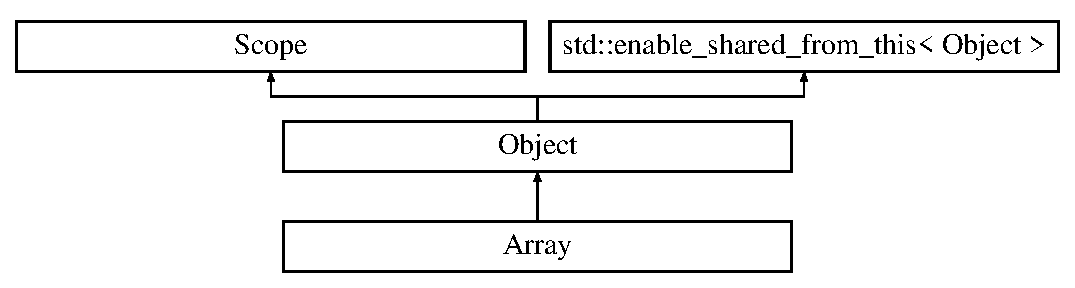
\includegraphics[height=3.000000cm]{classArray}
\end{center}
\end{figure}
\subsection*{Public Member Functions}
\begin{DoxyCompactItemize}
\item 
\hyperlink{classArray_a6bf7af2f8348ab6b96a656c2f2ea27ed}{Array} (\hyperlink{classInterpreter}{Interpreter} $\ast$interpreter, \hyperlink{classClass}{Class} $\ast$c, \hyperlink{classVariable}{Variable} $\ast$\hyperlink{classArray_af685a2298bef03e179093d6791c75b40}{variables}, int \hyperlink{classArray_a11dfcc73b3484e2bfdb5ce81457a7650}{count})
\item 
virtual \hyperlink{classArray_a66d3fee8e78097d35709028b3ba02803}{$\sim$\+Array} ()
\item 
virtual void \hyperlink{classArray_ac9828e89510c879b36acc6eca5efef51}{setup} ()
\end{DoxyCompactItemize}
\subsection*{Public Attributes}
\begin{DoxyCompactItemize}
\item 
\hyperlink{classVariable}{Variable} $\ast$ \hyperlink{classArray_af685a2298bef03e179093d6791c75b40}{variables}
\item 
int \hyperlink{classArray_a11dfcc73b3484e2bfdb5ce81457a7650}{count}
\end{DoxyCompactItemize}


\subsection{Constructor \& Destructor Documentation}
\mbox{\Hypertarget{classArray_a6bf7af2f8348ab6b96a656c2f2ea27ed}\label{classArray_a6bf7af2f8348ab6b96a656c2f2ea27ed}} 
\index{Array@{Array}!Array@{Array}}
\index{Array@{Array}!Array@{Array}}
\subsubsection{\texorpdfstring{Array()}{Array()}}
{\footnotesize\ttfamily Array\+::\+Array (\begin{DoxyParamCaption}\item[{\hyperlink{classInterpreter}{Interpreter} $\ast$}]{interpreter,  }\item[{\hyperlink{classClass}{Class} $\ast$}]{c,  }\item[{\hyperlink{classVariable}{Variable} $\ast$}]{variables,  }\item[{int}]{count }\end{DoxyParamCaption})}

\mbox{\Hypertarget{classArray_a66d3fee8e78097d35709028b3ba02803}\label{classArray_a66d3fee8e78097d35709028b3ba02803}} 
\index{Array@{Array}!````~Array@{$\sim$\+Array}}
\index{````~Array@{$\sim$\+Array}!Array@{Array}}
\subsubsection{\texorpdfstring{$\sim$\+Array()}{~Array()}}
{\footnotesize\ttfamily virtual Array\+::$\sim$\+Array (\begin{DoxyParamCaption}{ }\end{DoxyParamCaption})\hspace{0.3cm}{\ttfamily [virtual]}}



\subsection{Member Function Documentation}
\mbox{\Hypertarget{classArray_ac9828e89510c879b36acc6eca5efef51}\label{classArray_ac9828e89510c879b36acc6eca5efef51}} 
\index{Array@{Array}!setup@{setup}}
\index{setup@{setup}!Array@{Array}}
\subsubsection{\texorpdfstring{setup()}{setup()}}
{\footnotesize\ttfamily virtual void Array\+::setup (\begin{DoxyParamCaption}{ }\end{DoxyParamCaption})\hspace{0.3cm}{\ttfamily [virtual]}}



\subsection{Member Data Documentation}
\mbox{\Hypertarget{classArray_a11dfcc73b3484e2bfdb5ce81457a7650}\label{classArray_a11dfcc73b3484e2bfdb5ce81457a7650}} 
\index{Array@{Array}!count@{count}}
\index{count@{count}!Array@{Array}}
\subsubsection{\texorpdfstring{count}{count}}
{\footnotesize\ttfamily int Array\+::count}

\mbox{\Hypertarget{classArray_af685a2298bef03e179093d6791c75b40}\label{classArray_af685a2298bef03e179093d6791c75b40}} 
\index{Array@{Array}!variables@{variables}}
\index{variables@{variables}!Array@{Array}}
\subsubsection{\texorpdfstring{variables}{variables}}
{\footnotesize\ttfamily \hyperlink{classVariable}{Variable}$\ast$ Array\+::variables}



The documentation for this class was generated from the following file\+:\begin{DoxyCompactItemize}
\item 
include/\hyperlink{array_8h}{array.\+h}\end{DoxyCompactItemize}

\hypertarget{classArrayNode}{}\section{Array\+Node Class Reference}
\label{classArrayNode}\index{Array\+Node@{Array\+Node}}


{\ttfamily \#include $<$arraynode.\+h$>$}

Inheritance diagram for Array\+Node\+:\begin{figure}[H]
\begin{center}
\leavevmode
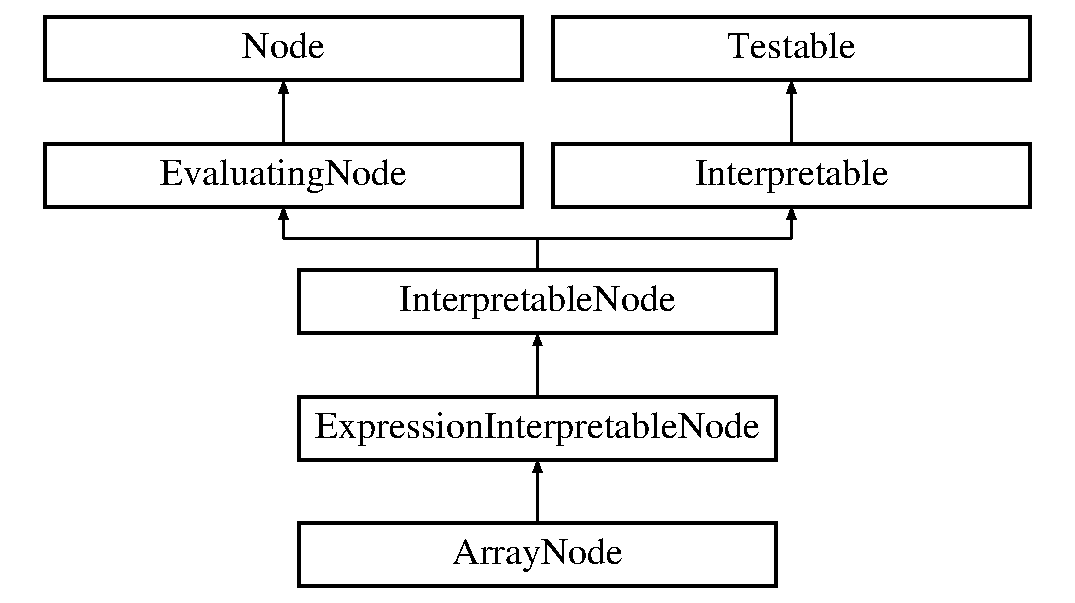
\includegraphics[height=5.000000cm]{classArrayNode}
\end{center}
\end{figure}
\subsection*{Public Member Functions}
\begin{DoxyCompactItemize}
\item 
\hyperlink{classArrayNode_adfb4eb2c05953007bb2af001141a2109}{Array\+Node} ()
\item 
virtual \hyperlink{classArrayNode_aa45e4fbc84eab2f8731feefdc99bd639}{$\sim$\+Array\+Node} ()
\item 
virtual \hyperlink{classValue}{Value} \hyperlink{classArrayNode_a029220b946233e22cb661fcfac9634d0}{interpret} (\hyperlink{classInterpreter}{Interpreter} $\ast$interpreter)
\end{DoxyCompactItemize}
\subsection*{Public Attributes}
\begin{DoxyCompactItemize}
\item 
\hyperlink{classExpressionInterpretableNode}{Expression\+Interpretable\+Node} $\ast$ \hyperlink{classArrayNode_a949140f67149544aec59044dcae07036}{index\+\_\+node}
\item 
\hyperlink{classNode}{Node} $\ast$ \hyperlink{classArrayNode_aa3bccfaecfe5597fd494ee56cae918dd}{next\+\_\+element}
\end{DoxyCompactItemize}
\subsection*{Additional Inherited Members}


\subsection{Constructor \& Destructor Documentation}
\mbox{\Hypertarget{classArrayNode_adfb4eb2c05953007bb2af001141a2109}\label{classArrayNode_adfb4eb2c05953007bb2af001141a2109}} 
\index{Array\+Node@{Array\+Node}!Array\+Node@{Array\+Node}}
\index{Array\+Node@{Array\+Node}!Array\+Node@{Array\+Node}}
\subsubsection{\texorpdfstring{Array\+Node()}{ArrayNode()}}
{\footnotesize\ttfamily Array\+Node\+::\+Array\+Node (\begin{DoxyParamCaption}{ }\end{DoxyParamCaption})}

\mbox{\Hypertarget{classArrayNode_aa45e4fbc84eab2f8731feefdc99bd639}\label{classArrayNode_aa45e4fbc84eab2f8731feefdc99bd639}} 
\index{Array\+Node@{Array\+Node}!````~Array\+Node@{$\sim$\+Array\+Node}}
\index{````~Array\+Node@{$\sim$\+Array\+Node}!Array\+Node@{Array\+Node}}
\subsubsection{\texorpdfstring{$\sim$\+Array\+Node()}{~ArrayNode()}}
{\footnotesize\ttfamily virtual Array\+Node\+::$\sim$\+Array\+Node (\begin{DoxyParamCaption}{ }\end{DoxyParamCaption})\hspace{0.3cm}{\ttfamily [virtual]}}



\subsection{Member Function Documentation}
\mbox{\Hypertarget{classArrayNode_a029220b946233e22cb661fcfac9634d0}\label{classArrayNode_a029220b946233e22cb661fcfac9634d0}} 
\index{Array\+Node@{Array\+Node}!interpret@{interpret}}
\index{interpret@{interpret}!Array\+Node@{Array\+Node}}
\subsubsection{\texorpdfstring{interpret()}{interpret()}}
{\footnotesize\ttfamily virtual \hyperlink{classValue}{Value} Array\+Node\+::interpret (\begin{DoxyParamCaption}\item[{\hyperlink{classInterpreter}{Interpreter} $\ast$}]{interpreter }\end{DoxyParamCaption})\hspace{0.3cm}{\ttfamily [virtual]}}



Implements \hyperlink{classExpressionInterpretableNode_a43650f046c48fc539f77a207e3c9181e}{Expression\+Interpretable\+Node}.



\subsection{Member Data Documentation}
\mbox{\Hypertarget{classArrayNode_a949140f67149544aec59044dcae07036}\label{classArrayNode_a949140f67149544aec59044dcae07036}} 
\index{Array\+Node@{Array\+Node}!index\+\_\+node@{index\+\_\+node}}
\index{index\+\_\+node@{index\+\_\+node}!Array\+Node@{Array\+Node}}
\subsubsection{\texorpdfstring{index\+\_\+node}{index\_node}}
{\footnotesize\ttfamily \hyperlink{classExpressionInterpretableNode}{Expression\+Interpretable\+Node}$\ast$ Array\+Node\+::index\+\_\+node}

\mbox{\Hypertarget{classArrayNode_aa3bccfaecfe5597fd494ee56cae918dd}\label{classArrayNode_aa3bccfaecfe5597fd494ee56cae918dd}} 
\index{Array\+Node@{Array\+Node}!next\+\_\+element@{next\+\_\+element}}
\index{next\+\_\+element@{next\+\_\+element}!Array\+Node@{Array\+Node}}
\subsubsection{\texorpdfstring{next\+\_\+element}{next\_element}}
{\footnotesize\ttfamily \hyperlink{classNode}{Node}$\ast$ Array\+Node\+::next\+\_\+element}



The documentation for this class was generated from the following file\+:\begin{DoxyCompactItemize}
\item 
include/\hyperlink{arraynode_8h}{arraynode.\+h}\end{DoxyCompactItemize}

\hypertarget{classBodyNode}{}\section{Body\+Node Class Reference}
\label{classBodyNode}\index{Body\+Node@{Body\+Node}}


{\ttfamily \#include $<$bodynode.\+h$>$}

Inheritance diagram for Body\+Node\+:\begin{figure}[H]
\begin{center}
\leavevmode
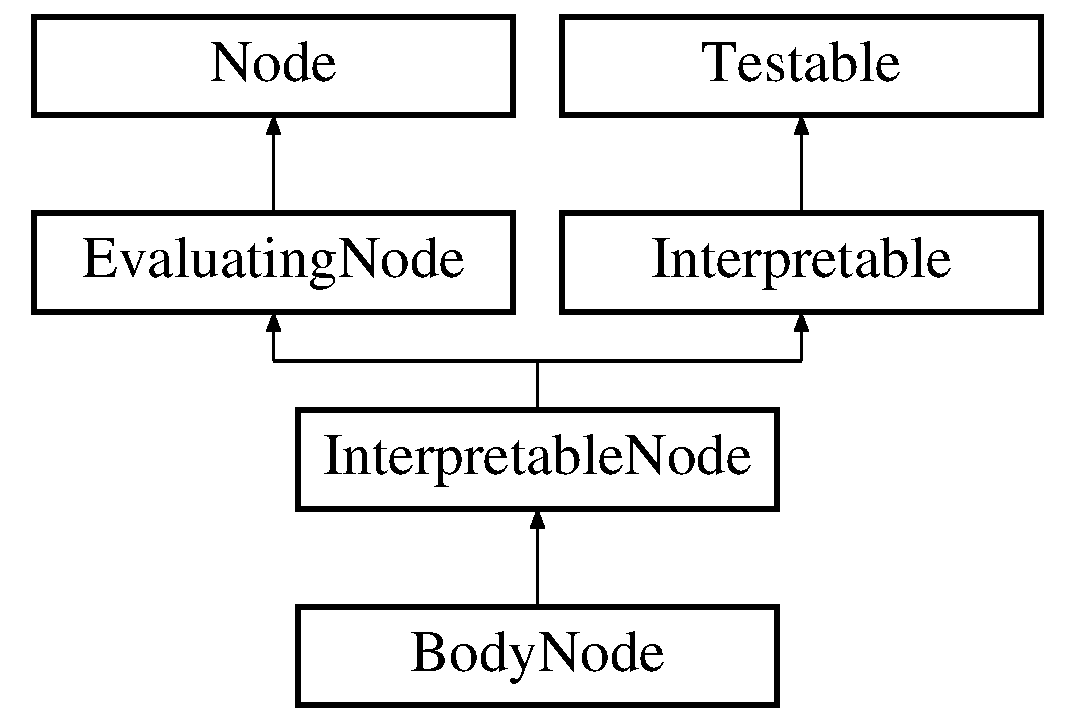
\includegraphics[height=4.000000cm]{classBodyNode}
\end{center}
\end{figure}
\subsection*{Public Member Functions}
\begin{DoxyCompactItemize}
\item 
\hyperlink{classBodyNode_ac431b406e16e66745f5413eb868f23b8}{Body\+Node} ()
\item 
virtual \hyperlink{classBodyNode_acf86c2f7982224510b39a5f35de0bbde}{$\sim$\+Body\+Node} ()
\item 
virtual void \hyperlink{classBodyNode_a80e75b0ab6c388c34a82bdce63fdc7bb}{test} (\hyperlink{classValidator}{Validator} $\ast$validator)
\item 
virtual \hyperlink{classValue}{Value} \hyperlink{classBodyNode_a5ab94984d059dba1f7d2baa6022712ba}{interpret} (\hyperlink{classInterpreter}{Interpreter} $\ast$interpreter)
\item 
virtual void \hyperlink{classBodyNode_ab08c6586b725065afca095786b842991}{evaluate\+\_\+impl} (\hyperlink{classSystemHandler}{System\+Handler} $\ast$handler, \hyperlink{statics_8h_a6664c451ca7787483a7981cc1de68dbb}{E\+V\+A\+L\+U\+A\+T\+I\+O\+N\+\_\+\+T\+Y\+PE} expected\+\_\+evaluation, struct \hyperlink{structEvaluation}{Evaluation} $\ast$evaluation)
\item 
void \hyperlink{classBodyNode_a8b27949f189186af47dd81336d0d5ce7}{on\+Before\+Leave} (std\+::function$<$ void()$>$ before\+\_\+leave\+\_\+function)
\item 
void \hyperlink{classBodyNode_adf1536979d1a57a735cc75290117afa4}{apply\+\_\+node\+\_\+listener} (std\+::function$<$ bool(\hyperlink{classNode}{Node} $\ast$node, \hyperlink{classValue}{Value} v)$>$ node\+\_\+listener\+\_\+function)
\item 
bool \hyperlink{classBodyNode_a7019e16f431cbf8975b1fde622d47d77}{interpret\+\_\+body\+\_\+node} (\hyperlink{classNode}{Node} $\ast$node)
\item 
void \hyperlink{classBodyNode_a9b6bafc8338e35a034aff1a23d519b1e}{interpret\+\_\+body} (\hyperlink{classBodyNode}{Body\+Node} $\ast$node)
\item 
void \hyperlink{classBodyNode_ab8a99f9e2c7d33f7cf4cbb07a61bec0f}{add\+Child} (\hyperlink{classInterpretableNode}{Interpretable\+Node} $\ast$c)
\end{DoxyCompactItemize}
\subsection*{Public Attributes}
\begin{DoxyCompactItemize}
\item 
\hyperlink{classInterpretableNode}{Interpretable\+Node} $\ast$ \hyperlink{classBodyNode_a6b18b29807903661a9f06e865331fca4}{child}
\end{DoxyCompactItemize}
\subsection*{Additional Inherited Members}


\subsection{Constructor \& Destructor Documentation}
\mbox{\Hypertarget{classBodyNode_ac431b406e16e66745f5413eb868f23b8}\label{classBodyNode_ac431b406e16e66745f5413eb868f23b8}} 
\index{Body\+Node@{Body\+Node}!Body\+Node@{Body\+Node}}
\index{Body\+Node@{Body\+Node}!Body\+Node@{Body\+Node}}
\subsubsection{\texorpdfstring{Body\+Node()}{BodyNode()}}
{\footnotesize\ttfamily Body\+Node\+::\+Body\+Node (\begin{DoxyParamCaption}{ }\end{DoxyParamCaption})}

\mbox{\Hypertarget{classBodyNode_acf86c2f7982224510b39a5f35de0bbde}\label{classBodyNode_acf86c2f7982224510b39a5f35de0bbde}} 
\index{Body\+Node@{Body\+Node}!````~Body\+Node@{$\sim$\+Body\+Node}}
\index{````~Body\+Node@{$\sim$\+Body\+Node}!Body\+Node@{Body\+Node}}
\subsubsection{\texorpdfstring{$\sim$\+Body\+Node()}{~BodyNode()}}
{\footnotesize\ttfamily virtual Body\+Node\+::$\sim$\+Body\+Node (\begin{DoxyParamCaption}{ }\end{DoxyParamCaption})\hspace{0.3cm}{\ttfamily [virtual]}}



\subsection{Member Function Documentation}
\mbox{\Hypertarget{classBodyNode_ab8a99f9e2c7d33f7cf4cbb07a61bec0f}\label{classBodyNode_ab8a99f9e2c7d33f7cf4cbb07a61bec0f}} 
\index{Body\+Node@{Body\+Node}!add\+Child@{add\+Child}}
\index{add\+Child@{add\+Child}!Body\+Node@{Body\+Node}}
\subsubsection{\texorpdfstring{add\+Child()}{addChild()}}
{\footnotesize\ttfamily void Body\+Node\+::add\+Child (\begin{DoxyParamCaption}\item[{\hyperlink{classInterpretableNode}{Interpretable\+Node} $\ast$}]{c }\end{DoxyParamCaption})}

\mbox{\Hypertarget{classBodyNode_adf1536979d1a57a735cc75290117afa4}\label{classBodyNode_adf1536979d1a57a735cc75290117afa4}} 
\index{Body\+Node@{Body\+Node}!apply\+\_\+node\+\_\+listener@{apply\+\_\+node\+\_\+listener}}
\index{apply\+\_\+node\+\_\+listener@{apply\+\_\+node\+\_\+listener}!Body\+Node@{Body\+Node}}
\subsubsection{\texorpdfstring{apply\+\_\+node\+\_\+listener()}{apply\_node\_listener()}}
{\footnotesize\ttfamily void Body\+Node\+::apply\+\_\+node\+\_\+listener (\begin{DoxyParamCaption}\item[{std\+::function$<$ bool(\hyperlink{classNode}{Node} $\ast$node, \hyperlink{classValue}{Value} v)$>$}]{node\+\_\+listener\+\_\+function }\end{DoxyParamCaption})}

\mbox{\Hypertarget{classBodyNode_ab08c6586b725065afca095786b842991}\label{classBodyNode_ab08c6586b725065afca095786b842991}} 
\index{Body\+Node@{Body\+Node}!evaluate\+\_\+impl@{evaluate\+\_\+impl}}
\index{evaluate\+\_\+impl@{evaluate\+\_\+impl}!Body\+Node@{Body\+Node}}
\subsubsection{\texorpdfstring{evaluate\+\_\+impl()}{evaluate\_impl()}}
{\footnotesize\ttfamily virtual void Body\+Node\+::evaluate\+\_\+impl (\begin{DoxyParamCaption}\item[{\hyperlink{classSystemHandler}{System\+Handler} $\ast$}]{handler,  }\item[{\hyperlink{statics_8h_a6664c451ca7787483a7981cc1de68dbb}{E\+V\+A\+L\+U\+A\+T\+I\+O\+N\+\_\+\+T\+Y\+PE}}]{expected\+\_\+evaluation,  }\item[{struct \hyperlink{structEvaluation}{Evaluation} $\ast$}]{evaluation }\end{DoxyParamCaption})\hspace{0.3cm}{\ttfamily [virtual]}}



Implements \hyperlink{classEvaluatingNode_a085fa06e0b46a93c814dc55cda0c1b26}{Evaluating\+Node}.

\mbox{\Hypertarget{classBodyNode_a5ab94984d059dba1f7d2baa6022712ba}\label{classBodyNode_a5ab94984d059dba1f7d2baa6022712ba}} 
\index{Body\+Node@{Body\+Node}!interpret@{interpret}}
\index{interpret@{interpret}!Body\+Node@{Body\+Node}}
\subsubsection{\texorpdfstring{interpret()}{interpret()}}
{\footnotesize\ttfamily virtual \hyperlink{classValue}{Value} Body\+Node\+::interpret (\begin{DoxyParamCaption}\item[{\hyperlink{classInterpreter}{Interpreter} $\ast$}]{interpreter }\end{DoxyParamCaption})\hspace{0.3cm}{\ttfamily [virtual]}}



Implements \hyperlink{classInterpretableNode_a9a466e7d65c4b323d2b96b4ac8396cd7}{Interpretable\+Node}.

\mbox{\Hypertarget{classBodyNode_a9b6bafc8338e35a034aff1a23d519b1e}\label{classBodyNode_a9b6bafc8338e35a034aff1a23d519b1e}} 
\index{Body\+Node@{Body\+Node}!interpret\+\_\+body@{interpret\+\_\+body}}
\index{interpret\+\_\+body@{interpret\+\_\+body}!Body\+Node@{Body\+Node}}
\subsubsection{\texorpdfstring{interpret\+\_\+body()}{interpret\_body()}}
{\footnotesize\ttfamily void Body\+Node\+::interpret\+\_\+body (\begin{DoxyParamCaption}\item[{\hyperlink{classBodyNode}{Body\+Node} $\ast$}]{node }\end{DoxyParamCaption})}

\mbox{\Hypertarget{classBodyNode_a7019e16f431cbf8975b1fde622d47d77}\label{classBodyNode_a7019e16f431cbf8975b1fde622d47d77}} 
\index{Body\+Node@{Body\+Node}!interpret\+\_\+body\+\_\+node@{interpret\+\_\+body\+\_\+node}}
\index{interpret\+\_\+body\+\_\+node@{interpret\+\_\+body\+\_\+node}!Body\+Node@{Body\+Node}}
\subsubsection{\texorpdfstring{interpret\+\_\+body\+\_\+node()}{interpret\_body\_node()}}
{\footnotesize\ttfamily bool Body\+Node\+::interpret\+\_\+body\+\_\+node (\begin{DoxyParamCaption}\item[{\hyperlink{classNode}{Node} $\ast$}]{node }\end{DoxyParamCaption})}

\mbox{\Hypertarget{classBodyNode_a8b27949f189186af47dd81336d0d5ce7}\label{classBodyNode_a8b27949f189186af47dd81336d0d5ce7}} 
\index{Body\+Node@{Body\+Node}!on\+Before\+Leave@{on\+Before\+Leave}}
\index{on\+Before\+Leave@{on\+Before\+Leave}!Body\+Node@{Body\+Node}}
\subsubsection{\texorpdfstring{on\+Before\+Leave()}{onBeforeLeave()}}
{\footnotesize\ttfamily void Body\+Node\+::on\+Before\+Leave (\begin{DoxyParamCaption}\item[{std\+::function$<$ void()$>$}]{before\+\_\+leave\+\_\+function }\end{DoxyParamCaption})}

\mbox{\Hypertarget{classBodyNode_a80e75b0ab6c388c34a82bdce63fdc7bb}\label{classBodyNode_a80e75b0ab6c388c34a82bdce63fdc7bb}} 
\index{Body\+Node@{Body\+Node}!test@{test}}
\index{test@{test}!Body\+Node@{Body\+Node}}
\subsubsection{\texorpdfstring{test()}{test()}}
{\footnotesize\ttfamily virtual void Body\+Node\+::test (\begin{DoxyParamCaption}\item[{\hyperlink{classValidator}{Validator} $\ast$}]{validator }\end{DoxyParamCaption})\hspace{0.3cm}{\ttfamily [virtual]}}



Reimplemented from \hyperlink{classInterpretable_a32f547aaf68dcbab993284d3257ab010}{Interpretable}.



\subsection{Member Data Documentation}
\mbox{\Hypertarget{classBodyNode_a6b18b29807903661a9f06e865331fca4}\label{classBodyNode_a6b18b29807903661a9f06e865331fca4}} 
\index{Body\+Node@{Body\+Node}!child@{child}}
\index{child@{child}!Body\+Node@{Body\+Node}}
\subsubsection{\texorpdfstring{child}{child}}
{\footnotesize\ttfamily \hyperlink{classInterpretableNode}{Interpretable\+Node}$\ast$ Body\+Node\+::child}



The documentation for this class was generated from the following file\+:\begin{DoxyCompactItemize}
\item 
include/\hyperlink{bodynode_8h}{bodynode.\+h}\end{DoxyCompactItemize}

\hypertarget{classCastNode}{}\section{Cast\+Node Class Reference}
\label{classCastNode}\index{Cast\+Node@{Cast\+Node}}


{\ttfamily \#include $<$castnode.\+h$>$}

Inheritance diagram for Cast\+Node\+:\begin{figure}[H]
\begin{center}
\leavevmode
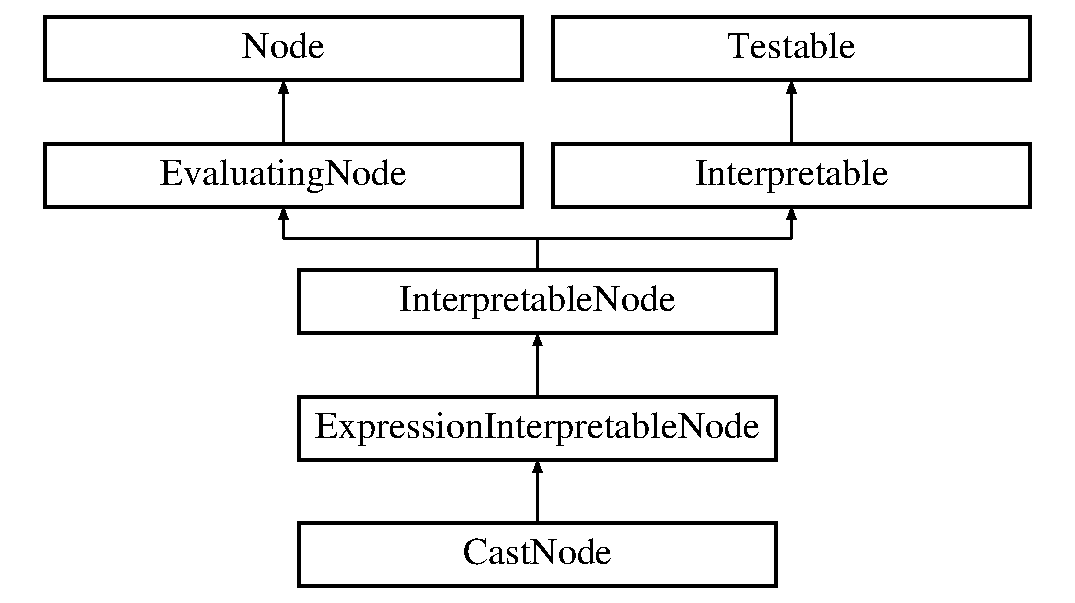
\includegraphics[height=5.000000cm]{classCastNode}
\end{center}
\end{figure}
\subsection*{Public Member Functions}
\begin{DoxyCompactItemize}
\item 
\hyperlink{classCastNode_aacc7aea8e67a26de47f9a9a175cad3e2}{Cast\+Node} ()
\item 
virtual \hyperlink{classCastNode_a358bc9d180542920fced2b7f35ef3f9f}{$\sim$\+Cast\+Node} ()
\item 
virtual \hyperlink{classValue}{Value} \hyperlink{classCastNode_a2a909a7531791bcbc53c514a01ce5024}{interpret} (\hyperlink{classInterpreter}{Interpreter} $\ast$interpreter)
\item 
virtual void \hyperlink{classCastNode_a19fa03c324a6dcbadac32965a86afb3e}{test} (\hyperlink{classValidator}{Validator} $\ast$validator)
\item 
virtual void \hyperlink{classCastNode_ae0c32d5d076c2572fa7afc9cb1a76a79}{evaluate\+\_\+impl} (\hyperlink{classSystemHandler}{System\+Handler} $\ast$handler, \hyperlink{statics_8h_a6664c451ca7787483a7981cc1de68dbb}{E\+V\+A\+L\+U\+A\+T\+I\+O\+N\+\_\+\+T\+Y\+PE} expected\+\_\+evaluation, struct \hyperlink{structEvaluation}{Evaluation} $\ast$evaluation)
\end{DoxyCompactItemize}
\subsection*{Public Attributes}
\begin{DoxyCompactItemize}
\item 
\hyperlink{classEvaluatingNode}{Evaluating\+Node} $\ast$ \hyperlink{classCastNode_adc7612dd690f94026adeea0d98970b57}{casting\+\_\+to}
\item 
\hyperlink{classExpressionInterpretableNode}{Expression\+Interpretable\+Node} $\ast$ \hyperlink{classCastNode_a01fc0556ce65230a77941f1519b72769}{to\+\_\+cast}
\end{DoxyCompactItemize}
\subsection*{Additional Inherited Members}


\subsection{Constructor \& Destructor Documentation}
\mbox{\Hypertarget{classCastNode_aacc7aea8e67a26de47f9a9a175cad3e2}\label{classCastNode_aacc7aea8e67a26de47f9a9a175cad3e2}} 
\index{Cast\+Node@{Cast\+Node}!Cast\+Node@{Cast\+Node}}
\index{Cast\+Node@{Cast\+Node}!Cast\+Node@{Cast\+Node}}
\subsubsection{\texorpdfstring{Cast\+Node()}{CastNode()}}
{\footnotesize\ttfamily Cast\+Node\+::\+Cast\+Node (\begin{DoxyParamCaption}{ }\end{DoxyParamCaption})}

\mbox{\Hypertarget{classCastNode_a358bc9d180542920fced2b7f35ef3f9f}\label{classCastNode_a358bc9d180542920fced2b7f35ef3f9f}} 
\index{Cast\+Node@{Cast\+Node}!````~Cast\+Node@{$\sim$\+Cast\+Node}}
\index{````~Cast\+Node@{$\sim$\+Cast\+Node}!Cast\+Node@{Cast\+Node}}
\subsubsection{\texorpdfstring{$\sim$\+Cast\+Node()}{~CastNode()}}
{\footnotesize\ttfamily virtual Cast\+Node\+::$\sim$\+Cast\+Node (\begin{DoxyParamCaption}{ }\end{DoxyParamCaption})\hspace{0.3cm}{\ttfamily [virtual]}}



\subsection{Member Function Documentation}
\mbox{\Hypertarget{classCastNode_ae0c32d5d076c2572fa7afc9cb1a76a79}\label{classCastNode_ae0c32d5d076c2572fa7afc9cb1a76a79}} 
\index{Cast\+Node@{Cast\+Node}!evaluate\+\_\+impl@{evaluate\+\_\+impl}}
\index{evaluate\+\_\+impl@{evaluate\+\_\+impl}!Cast\+Node@{Cast\+Node}}
\subsubsection{\texorpdfstring{evaluate\+\_\+impl()}{evaluate\_impl()}}
{\footnotesize\ttfamily virtual void Cast\+Node\+::evaluate\+\_\+impl (\begin{DoxyParamCaption}\item[{\hyperlink{classSystemHandler}{System\+Handler} $\ast$}]{handler,  }\item[{\hyperlink{statics_8h_a6664c451ca7787483a7981cc1de68dbb}{E\+V\+A\+L\+U\+A\+T\+I\+O\+N\+\_\+\+T\+Y\+PE}}]{expected\+\_\+evaluation,  }\item[{struct \hyperlink{structEvaluation}{Evaluation} $\ast$}]{evaluation }\end{DoxyParamCaption})\hspace{0.3cm}{\ttfamily [virtual]}}



Implements \hyperlink{classEvaluatingNode_a085fa06e0b46a93c814dc55cda0c1b26}{Evaluating\+Node}.

\mbox{\Hypertarget{classCastNode_a2a909a7531791bcbc53c514a01ce5024}\label{classCastNode_a2a909a7531791bcbc53c514a01ce5024}} 
\index{Cast\+Node@{Cast\+Node}!interpret@{interpret}}
\index{interpret@{interpret}!Cast\+Node@{Cast\+Node}}
\subsubsection{\texorpdfstring{interpret()}{interpret()}}
{\footnotesize\ttfamily virtual \hyperlink{classValue}{Value} Cast\+Node\+::interpret (\begin{DoxyParamCaption}\item[{\hyperlink{classInterpreter}{Interpreter} $\ast$}]{interpreter }\end{DoxyParamCaption})\hspace{0.3cm}{\ttfamily [virtual]}}



Implements \hyperlink{classExpressionInterpretableNode_a43650f046c48fc539f77a207e3c9181e}{Expression\+Interpretable\+Node}.

\mbox{\Hypertarget{classCastNode_a19fa03c324a6dcbadac32965a86afb3e}\label{classCastNode_a19fa03c324a6dcbadac32965a86afb3e}} 
\index{Cast\+Node@{Cast\+Node}!test@{test}}
\index{test@{test}!Cast\+Node@{Cast\+Node}}
\subsubsection{\texorpdfstring{test()}{test()}}
{\footnotesize\ttfamily virtual void Cast\+Node\+::test (\begin{DoxyParamCaption}\item[{\hyperlink{classValidator}{Validator} $\ast$}]{validator }\end{DoxyParamCaption})\hspace{0.3cm}{\ttfamily [virtual]}}



Reimplemented from \hyperlink{classInterpretable_a32f547aaf68dcbab993284d3257ab010}{Interpretable}.



\subsection{Member Data Documentation}
\mbox{\Hypertarget{classCastNode_adc7612dd690f94026adeea0d98970b57}\label{classCastNode_adc7612dd690f94026adeea0d98970b57}} 
\index{Cast\+Node@{Cast\+Node}!casting\+\_\+to@{casting\+\_\+to}}
\index{casting\+\_\+to@{casting\+\_\+to}!Cast\+Node@{Cast\+Node}}
\subsubsection{\texorpdfstring{casting\+\_\+to}{casting\_to}}
{\footnotesize\ttfamily \hyperlink{classEvaluatingNode}{Evaluating\+Node}$\ast$ Cast\+Node\+::casting\+\_\+to}

\mbox{\Hypertarget{classCastNode_a01fc0556ce65230a77941f1519b72769}\label{classCastNode_a01fc0556ce65230a77941f1519b72769}} 
\index{Cast\+Node@{Cast\+Node}!to\+\_\+cast@{to\+\_\+cast}}
\index{to\+\_\+cast@{to\+\_\+cast}!Cast\+Node@{Cast\+Node}}
\subsubsection{\texorpdfstring{to\+\_\+cast}{to\_cast}}
{\footnotesize\ttfamily \hyperlink{classExpressionInterpretableNode}{Expression\+Interpretable\+Node}$\ast$ Cast\+Node\+::to\+\_\+cast}



The documentation for this class was generated from the following file\+:\begin{DoxyCompactItemize}
\item 
include/\hyperlink{castnode_8h}{castnode.\+h}\end{DoxyCompactItemize}

\hypertarget{classClass}{}\section{Class Class Reference}
\label{classClass}\index{Class@{Class}}


{\ttfamily \#include $<$class.\+h$>$}

Inheritance diagram for Class\+:\begin{figure}[H]
\begin{center}
\leavevmode
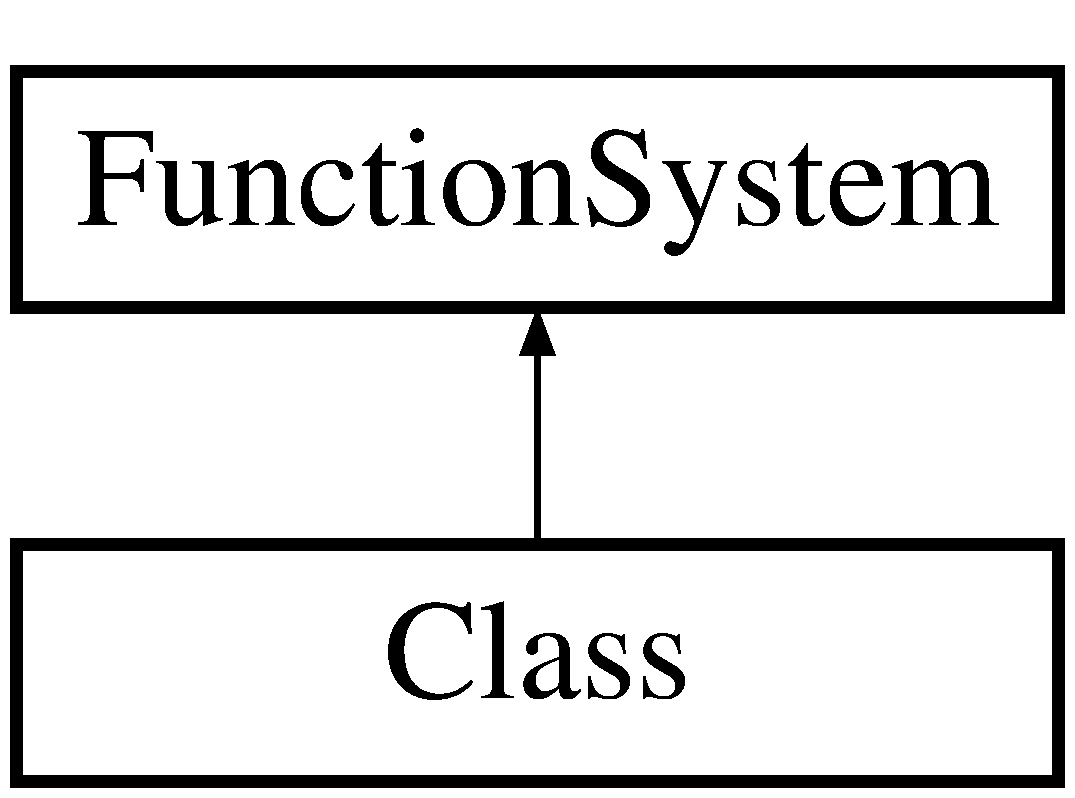
\includegraphics[height=2.000000cm]{classClass}
\end{center}
\end{figure}
\subsection*{Public Member Functions}
\begin{DoxyCompactItemize}
\item 
\hyperlink{classClass_a1c88be1af88c4c9b3c054d124ce44b6e}{Class} (\hyperlink{classSystemHandler}{System\+Handler} $\ast$sys\+\_\+handler, std\+::string \hyperlink{classClass_aac209ee2e03afc3bc9e93fd1fd46256b}{name}, \hyperlink{classFunctionSystem}{Function\+System} $\ast$prev\+\_\+fc\+\_\+sys)
\item 
\hyperlink{classClass_a1b960c202d43c46097e267e5c4e259ef}{Class} (\hyperlink{classSystemHandler}{System\+Handler} $\ast$sys\+\_\+handler, std\+::string \hyperlink{classClass_aac209ee2e03afc3bc9e93fd1fd46256b}{name}, \hyperlink{classClass}{Class} $\ast$\hyperlink{classClass_a1f94bc39c04d18b5c4421862f8506d1d}{parent})
\item 
virtual \hyperlink{classClass_aa3b9e4e0df41778f3d26777c1eb62898}{$\sim$\+Class} ()
\item 
virtual \hyperlink{classFunction}{Function} $\ast$ \hyperlink{classClass_a91798da1986d9f12a2d40a9997849542}{register\+Function} (std\+::string \hyperlink{classClass_aac209ee2e03afc3bc9e93fd1fd46256b}{name}, std\+::vector$<$ \hyperlink{classVarType}{Var\+Type} $>$ args, std\+::function$<$ void(std\+::vector$<$ \hyperlink{classValue}{Value} $>$ values, \hyperlink{classValue}{Value} $\ast$return\+\_\+value, std\+::shared\+\_\+ptr$<$ \hyperlink{classObject}{Object} $>$ object)$>$ entrypoint)
\item 
virtual \hyperlink{classFunction}{Function} $\ast$ \hyperlink{classClass_a757c7a4cb7e9e0b5486a087b953e919e}{register\+Function} (\hyperlink{classFunctionNode}{Function\+Node} $\ast$fnode)
\item 
void \hyperlink{classClass_a0c10b6fc7440f229da43f013271c0506}{add\+Variable} (\hyperlink{classVariable}{Variable} v)
\item 
bool \hyperlink{classClass_a0c5ffb0b7e3e95dedad01b8b4e91d93b}{has\+Variable\+With\+Name} (std\+::string \hyperlink{classClass_aac209ee2e03afc3bc9e93fd1fd46256b}{name})
\item 
\hyperlink{classVariable}{Variable} \hyperlink{classClass_a5c5de4f3c1419dedc92fc3d982fc6f65}{get\+Variable} (std\+::string \hyperlink{classClass_aac209ee2e03afc3bc9e93fd1fd46256b}{name})
\item 
std\+::vector$<$ \hyperlink{classVariable}{Variable} $>$ \hyperlink{classClass_ab24282751aa8b0ba2b2c71fbd3eef7e5}{get\+Variables} ()
\item 
\hyperlink{classClass}{Class} $\ast$ \hyperlink{classClass_aec836433f28bcfb9bf013ce79f24ba23}{get\+Class\+Who\+Has\+Variable} (std\+::string \hyperlink{classClass_aac209ee2e03afc3bc9e93fd1fd46256b}{name})
\item 
bool \hyperlink{classClass_a9bbffa241c269033a12c76f85af9c5ac}{instance\+Of} (\hyperlink{classClass}{Class} $\ast$c)
\end{DoxyCompactItemize}
\subsection*{Public Attributes}
\begin{DoxyCompactItemize}
\item 
std\+::string \hyperlink{classClass_aac209ee2e03afc3bc9e93fd1fd46256b}{name}
\item 
\hyperlink{classClass}{Class} $\ast$ \hyperlink{classClass_a1f94bc39c04d18b5c4421862f8506d1d}{parent}
\end{DoxyCompactItemize}


\subsection{Constructor \& Destructor Documentation}
\mbox{\Hypertarget{classClass_a1c88be1af88c4c9b3c054d124ce44b6e}\label{classClass_a1c88be1af88c4c9b3c054d124ce44b6e}} 
\index{Class@{Class}!Class@{Class}}
\index{Class@{Class}!Class@{Class}}
\subsubsection{\texorpdfstring{Class()}{Class()}\hspace{0.1cm}{\footnotesize\ttfamily [1/2]}}
{\footnotesize\ttfamily Class\+::\+Class (\begin{DoxyParamCaption}\item[{\hyperlink{classSystemHandler}{System\+Handler} $\ast$}]{sys\+\_\+handler,  }\item[{std\+::string}]{name,  }\item[{\hyperlink{classFunctionSystem}{Function\+System} $\ast$}]{prev\+\_\+fc\+\_\+sys }\end{DoxyParamCaption})}

\mbox{\Hypertarget{classClass_a1b960c202d43c46097e267e5c4e259ef}\label{classClass_a1b960c202d43c46097e267e5c4e259ef}} 
\index{Class@{Class}!Class@{Class}}
\index{Class@{Class}!Class@{Class}}
\subsubsection{\texorpdfstring{Class()}{Class()}\hspace{0.1cm}{\footnotesize\ttfamily [2/2]}}
{\footnotesize\ttfamily Class\+::\+Class (\begin{DoxyParamCaption}\item[{\hyperlink{classSystemHandler}{System\+Handler} $\ast$}]{sys\+\_\+handler,  }\item[{std\+::string}]{name,  }\item[{\hyperlink{classClass}{Class} $\ast$}]{parent }\end{DoxyParamCaption})}

\mbox{\Hypertarget{classClass_aa3b9e4e0df41778f3d26777c1eb62898}\label{classClass_aa3b9e4e0df41778f3d26777c1eb62898}} 
\index{Class@{Class}!````~Class@{$\sim$\+Class}}
\index{````~Class@{$\sim$\+Class}!Class@{Class}}
\subsubsection{\texorpdfstring{$\sim$\+Class()}{~Class()}}
{\footnotesize\ttfamily virtual Class\+::$\sim$\+Class (\begin{DoxyParamCaption}{ }\end{DoxyParamCaption})\hspace{0.3cm}{\ttfamily [virtual]}}



\subsection{Member Function Documentation}
\mbox{\Hypertarget{classClass_a0c10b6fc7440f229da43f013271c0506}\label{classClass_a0c10b6fc7440f229da43f013271c0506}} 
\index{Class@{Class}!add\+Variable@{add\+Variable}}
\index{add\+Variable@{add\+Variable}!Class@{Class}}
\subsubsection{\texorpdfstring{add\+Variable()}{addVariable()}}
{\footnotesize\ttfamily void Class\+::add\+Variable (\begin{DoxyParamCaption}\item[{\hyperlink{classVariable}{Variable}}]{v }\end{DoxyParamCaption})}

\mbox{\Hypertarget{classClass_aec836433f28bcfb9bf013ce79f24ba23}\label{classClass_aec836433f28bcfb9bf013ce79f24ba23}} 
\index{Class@{Class}!get\+Class\+Who\+Has\+Variable@{get\+Class\+Who\+Has\+Variable}}
\index{get\+Class\+Who\+Has\+Variable@{get\+Class\+Who\+Has\+Variable}!Class@{Class}}
\subsubsection{\texorpdfstring{get\+Class\+Who\+Has\+Variable()}{getClassWhoHasVariable()}}
{\footnotesize\ttfamily \hyperlink{classClass}{Class}$\ast$ Class\+::get\+Class\+Who\+Has\+Variable (\begin{DoxyParamCaption}\item[{std\+::string}]{name }\end{DoxyParamCaption})}

\mbox{\Hypertarget{classClass_a5c5de4f3c1419dedc92fc3d982fc6f65}\label{classClass_a5c5de4f3c1419dedc92fc3d982fc6f65}} 
\index{Class@{Class}!get\+Variable@{get\+Variable}}
\index{get\+Variable@{get\+Variable}!Class@{Class}}
\subsubsection{\texorpdfstring{get\+Variable()}{getVariable()}}
{\footnotesize\ttfamily \hyperlink{classVariable}{Variable} Class\+::get\+Variable (\begin{DoxyParamCaption}\item[{std\+::string}]{name }\end{DoxyParamCaption})}

\mbox{\Hypertarget{classClass_ab24282751aa8b0ba2b2c71fbd3eef7e5}\label{classClass_ab24282751aa8b0ba2b2c71fbd3eef7e5}} 
\index{Class@{Class}!get\+Variables@{get\+Variables}}
\index{get\+Variables@{get\+Variables}!Class@{Class}}
\subsubsection{\texorpdfstring{get\+Variables()}{getVariables()}}
{\footnotesize\ttfamily std\+::vector$<$\hyperlink{classVariable}{Variable}$>$ Class\+::get\+Variables (\begin{DoxyParamCaption}{ }\end{DoxyParamCaption})}

\mbox{\Hypertarget{classClass_a0c5ffb0b7e3e95dedad01b8b4e91d93b}\label{classClass_a0c5ffb0b7e3e95dedad01b8b4e91d93b}} 
\index{Class@{Class}!has\+Variable\+With\+Name@{has\+Variable\+With\+Name}}
\index{has\+Variable\+With\+Name@{has\+Variable\+With\+Name}!Class@{Class}}
\subsubsection{\texorpdfstring{has\+Variable\+With\+Name()}{hasVariableWithName()}}
{\footnotesize\ttfamily bool Class\+::has\+Variable\+With\+Name (\begin{DoxyParamCaption}\item[{std\+::string}]{name }\end{DoxyParamCaption})}

\mbox{\Hypertarget{classClass_a9bbffa241c269033a12c76f85af9c5ac}\label{classClass_a9bbffa241c269033a12c76f85af9c5ac}} 
\index{Class@{Class}!instance\+Of@{instance\+Of}}
\index{instance\+Of@{instance\+Of}!Class@{Class}}
\subsubsection{\texorpdfstring{instance\+Of()}{instanceOf()}}
{\footnotesize\ttfamily bool Class\+::instance\+Of (\begin{DoxyParamCaption}\item[{\hyperlink{classClass}{Class} $\ast$}]{c }\end{DoxyParamCaption})}

\mbox{\Hypertarget{classClass_a91798da1986d9f12a2d40a9997849542}\label{classClass_a91798da1986d9f12a2d40a9997849542}} 
\index{Class@{Class}!register\+Function@{register\+Function}}
\index{register\+Function@{register\+Function}!Class@{Class}}
\subsubsection{\texorpdfstring{register\+Function()}{registerFunction()}\hspace{0.1cm}{\footnotesize\ttfamily [1/2]}}
{\footnotesize\ttfamily virtual \hyperlink{classFunction}{Function}$\ast$ Class\+::register\+Function (\begin{DoxyParamCaption}\item[{std\+::string}]{name,  }\item[{std\+::vector$<$ \hyperlink{classVarType}{Var\+Type} $>$}]{args,  }\item[{std\+::function$<$ void(std\+::vector$<$ \hyperlink{classValue}{Value} $>$ values, \hyperlink{classValue}{Value} $\ast$return\+\_\+value, std\+::shared\+\_\+ptr$<$ \hyperlink{classObject}{Object} $>$ object)$>$}]{entrypoint }\end{DoxyParamCaption})\hspace{0.3cm}{\ttfamily [virtual]}}

Creates and registers a \hyperlink{classNativeFunction}{Native\+Function} into the \hyperlink{classFunctionSystem}{Function\+System} and when the function is called the {\bfseries entrypoint} lambda function provided will be invoked. 
\begin{DoxyParams}{Parameters}
{\em name} & The name of the function to create \\
\hline
{\em args} & The arguments this function takes. \\
\hline
{\em entrypoint} & The entrypoint of the function. \\
\hline
\end{DoxyParams}


Reimplemented from \hyperlink{classFunctionSystem_a37becc8c6067e6d7e4a1cc494e7d722f}{Function\+System}.

\mbox{\Hypertarget{classClass_a757c7a4cb7e9e0b5486a087b953e919e}\label{classClass_a757c7a4cb7e9e0b5486a087b953e919e}} 
\index{Class@{Class}!register\+Function@{register\+Function}}
\index{register\+Function@{register\+Function}!Class@{Class}}
\subsubsection{\texorpdfstring{register\+Function()}{registerFunction()}\hspace{0.1cm}{\footnotesize\ttfamily [2/2]}}
{\footnotesize\ttfamily virtual \hyperlink{classFunction}{Function}$\ast$ Class\+::register\+Function (\begin{DoxyParamCaption}\item[{\hyperlink{classFunctionNode}{Function\+Node} $\ast$}]{fnode }\end{DoxyParamCaption})\hspace{0.3cm}{\ttfamily [virtual]}}



Reimplemented from \hyperlink{classFunctionSystem_a7356903aa11df3b4c52f7d0c8f230d87}{Function\+System}.



\subsection{Member Data Documentation}
\mbox{\Hypertarget{classClass_aac209ee2e03afc3bc9e93fd1fd46256b}\label{classClass_aac209ee2e03afc3bc9e93fd1fd46256b}} 
\index{Class@{Class}!name@{name}}
\index{name@{name}!Class@{Class}}
\subsubsection{\texorpdfstring{name}{name}}
{\footnotesize\ttfamily std\+::string Class\+::name}

\mbox{\Hypertarget{classClass_a1f94bc39c04d18b5c4421862f8506d1d}\label{classClass_a1f94bc39c04d18b5c4421862f8506d1d}} 
\index{Class@{Class}!parent@{parent}}
\index{parent@{parent}!Class@{Class}}
\subsubsection{\texorpdfstring{parent}{parent}}
{\footnotesize\ttfamily \hyperlink{classClass}{Class}$\ast$ Class\+::parent}



The documentation for this class was generated from the following file\+:\begin{DoxyCompactItemize}
\item 
include/\hyperlink{class_8h}{class.\+h}\end{DoxyCompactItemize}

\hypertarget{classClassNode}{}\section{Class\+Node Class Reference}
\label{classClassNode}\index{Class\+Node@{Class\+Node}}


{\ttfamily \#include $<$classnode.\+h$>$}

Inheritance diagram for Class\+Node\+:\begin{figure}[H]
\begin{center}
\leavevmode
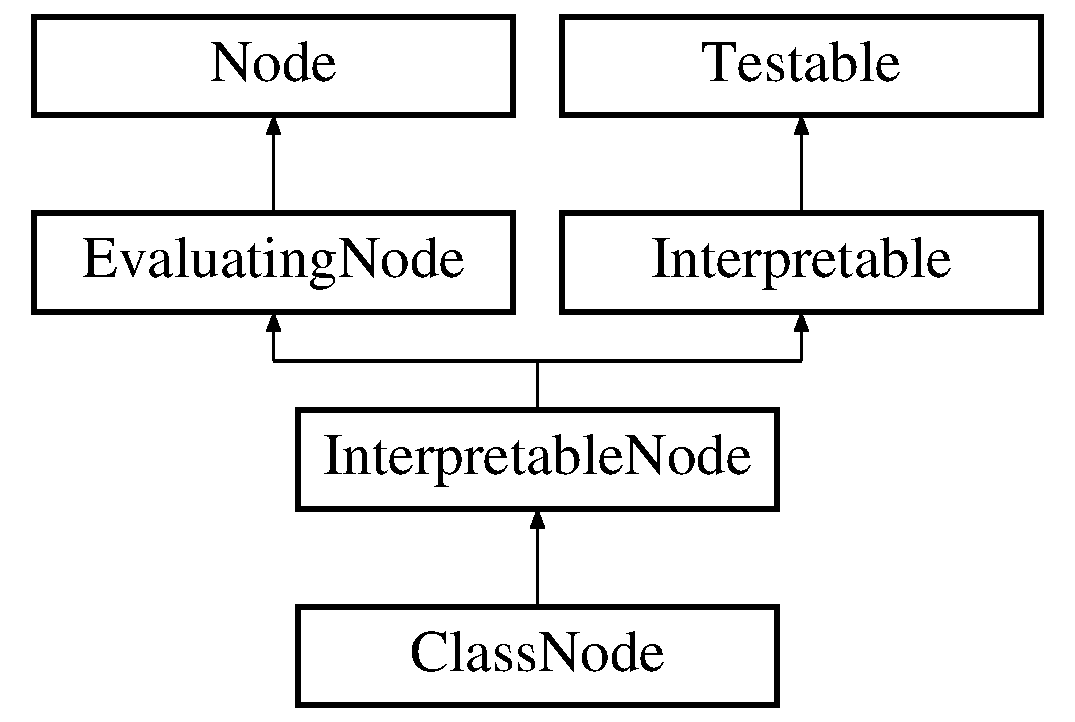
\includegraphics[height=4.000000cm]{classClassNode}
\end{center}
\end{figure}
\subsection*{Public Member Functions}
\begin{DoxyCompactItemize}
\item 
\hyperlink{classClassNode_a217389d155a37b90d12fa6a9d49d6326}{Class\+Node} ()
\item 
virtual \hyperlink{classClassNode_a3c0d617d08db3d2f0e9ade88f30bb04d}{$\sim$\+Class\+Node} ()
\item 
virtual void \hyperlink{classClassNode_ac5147024d81a0c6841e9453025e4f988}{test} (\hyperlink{classValidator}{Validator} $\ast$validator)
\item 
virtual \hyperlink{classValue}{Value} \hyperlink{classClassNode_a7515421face64d74e99e180fb297684b}{interpret} (\hyperlink{classInterpreter}{Interpreter} $\ast$interpreter)
\end{DoxyCompactItemize}
\subsection*{Public Attributes}
\begin{DoxyCompactItemize}
\item 
std\+::string \hyperlink{classClassNode_a1fc3152f6442b5f6913ec72f26afacbe}{name}
\item 
\hyperlink{classBodyNode}{Body\+Node} $\ast$ \hyperlink{classClassNode_ad5c089e050c2c7da583376fe16762689}{body}
\item 
std\+::string \hyperlink{classClassNode_a844a82eec88057b0faaf203f5a60a301}{parent}
\end{DoxyCompactItemize}
\subsection*{Additional Inherited Members}


\subsection{Constructor \& Destructor Documentation}
\mbox{\Hypertarget{classClassNode_a217389d155a37b90d12fa6a9d49d6326}\label{classClassNode_a217389d155a37b90d12fa6a9d49d6326}} 
\index{Class\+Node@{Class\+Node}!Class\+Node@{Class\+Node}}
\index{Class\+Node@{Class\+Node}!Class\+Node@{Class\+Node}}
\subsubsection{\texorpdfstring{Class\+Node()}{ClassNode()}}
{\footnotesize\ttfamily Class\+Node\+::\+Class\+Node (\begin{DoxyParamCaption}{ }\end{DoxyParamCaption})}

\mbox{\Hypertarget{classClassNode_a3c0d617d08db3d2f0e9ade88f30bb04d}\label{classClassNode_a3c0d617d08db3d2f0e9ade88f30bb04d}} 
\index{Class\+Node@{Class\+Node}!````~Class\+Node@{$\sim$\+Class\+Node}}
\index{````~Class\+Node@{$\sim$\+Class\+Node}!Class\+Node@{Class\+Node}}
\subsubsection{\texorpdfstring{$\sim$\+Class\+Node()}{~ClassNode()}}
{\footnotesize\ttfamily virtual Class\+Node\+::$\sim$\+Class\+Node (\begin{DoxyParamCaption}{ }\end{DoxyParamCaption})\hspace{0.3cm}{\ttfamily [virtual]}}



\subsection{Member Function Documentation}
\mbox{\Hypertarget{classClassNode_a7515421face64d74e99e180fb297684b}\label{classClassNode_a7515421face64d74e99e180fb297684b}} 
\index{Class\+Node@{Class\+Node}!interpret@{interpret}}
\index{interpret@{interpret}!Class\+Node@{Class\+Node}}
\subsubsection{\texorpdfstring{interpret()}{interpret()}}
{\footnotesize\ttfamily virtual \hyperlink{classValue}{Value} Class\+Node\+::interpret (\begin{DoxyParamCaption}\item[{\hyperlink{classInterpreter}{Interpreter} $\ast$}]{interpreter }\end{DoxyParamCaption})\hspace{0.3cm}{\ttfamily [virtual]}}



Implements \hyperlink{classInterpretableNode_a9a466e7d65c4b323d2b96b4ac8396cd7}{Interpretable\+Node}.

\mbox{\Hypertarget{classClassNode_ac5147024d81a0c6841e9453025e4f988}\label{classClassNode_ac5147024d81a0c6841e9453025e4f988}} 
\index{Class\+Node@{Class\+Node}!test@{test}}
\index{test@{test}!Class\+Node@{Class\+Node}}
\subsubsection{\texorpdfstring{test()}{test()}}
{\footnotesize\ttfamily virtual void Class\+Node\+::test (\begin{DoxyParamCaption}\item[{\hyperlink{classValidator}{Validator} $\ast$}]{validator }\end{DoxyParamCaption})\hspace{0.3cm}{\ttfamily [virtual]}}



Reimplemented from \hyperlink{classInterpretable_a32f547aaf68dcbab993284d3257ab010}{Interpretable}.



\subsection{Member Data Documentation}
\mbox{\Hypertarget{classClassNode_ad5c089e050c2c7da583376fe16762689}\label{classClassNode_ad5c089e050c2c7da583376fe16762689}} 
\index{Class\+Node@{Class\+Node}!body@{body}}
\index{body@{body}!Class\+Node@{Class\+Node}}
\subsubsection{\texorpdfstring{body}{body}}
{\footnotesize\ttfamily \hyperlink{classBodyNode}{Body\+Node}$\ast$ Class\+Node\+::body}

\mbox{\Hypertarget{classClassNode_a1fc3152f6442b5f6913ec72f26afacbe}\label{classClassNode_a1fc3152f6442b5f6913ec72f26afacbe}} 
\index{Class\+Node@{Class\+Node}!name@{name}}
\index{name@{name}!Class\+Node@{Class\+Node}}
\subsubsection{\texorpdfstring{name}{name}}
{\footnotesize\ttfamily std\+::string Class\+Node\+::name}

\mbox{\Hypertarget{classClassNode_a844a82eec88057b0faaf203f5a60a301}\label{classClassNode_a844a82eec88057b0faaf203f5a60a301}} 
\index{Class\+Node@{Class\+Node}!parent@{parent}}
\index{parent@{parent}!Class\+Node@{Class\+Node}}
\subsubsection{\texorpdfstring{parent}{parent}}
{\footnotesize\ttfamily std\+::string Class\+Node\+::parent}



The documentation for this class was generated from the following file\+:\begin{DoxyCompactItemize}
\item 
include/\hyperlink{classnode_8h}{classnode.\+h}\end{DoxyCompactItemize}

\hypertarget{classClassSystem}{}\section{Class\+System Class Reference}
\label{classClassSystem}\index{Class\+System@{Class\+System}}


{\ttfamily \#include $<$csystem.\+h$>$}

\subsection*{Public Member Functions}
\begin{DoxyCompactItemize}
\item 
\hyperlink{classClassSystem_aaaec70fea8c72ed8c47bfb4de3fc4b46}{Class\+System} ()
\item 
virtual \hyperlink{classClassSystem_a9b1842899a13f28ca47cf24287dc0616}{$\sim$\+Class\+System} ()
\item 
void \hyperlink{classClassSystem_abe7eb559b5291d324cb055c89e80b180}{set\+System\+Handler} (\hyperlink{classSystemHandler}{System\+Handler} $\ast$sys\+\_\+handler)
\item 
void \hyperlink{classClassSystem_a8bda9472a03697e442079606aa51c4fc}{set\+Previous\+Class\+System} (\hyperlink{classClassSystem}{Class\+System} $\ast$prev\+\_\+sys)
\item 
\hyperlink{classClassSystem}{Class\+System} $\ast$ \hyperlink{classClassSystem_a32c4883e03da6a11ab11f2f39afc073a}{get\+Previous\+Class\+System} ()
\item 
void \hyperlink{classClassSystem_a10283c2e4e7cc89b213f6a32a0d709c1}{set\+Default\+Base\+Class} (\hyperlink{classClass}{Class} $\ast$c)
\item 
\hyperlink{classClass}{Class} $\ast$ \hyperlink{classClassSystem_add1ff8eadba3826024e68c836af28250}{get\+Default\+Base\+Class} ()
\item 
\hyperlink{classClass}{Class} $\ast$ \hyperlink{classClassSystem_a02f4790dd9b8fa8808a4e17f1e152281}{register\+Class} (std\+::string class\+\_\+name, \hyperlink{classClass}{Class} $\ast$parent=N\+U\+LL)
\item 
\hyperlink{classClass}{Class} $\ast$ \hyperlink{classClassSystem_a4b88087eed035dc1f6100850c933ae84}{get\+Class\+By\+Name} (std\+::string name)
\item 
bool \hyperlink{classClassSystem_aa3e6fdac5739091d3f48dbe2b8c9db46}{has\+Class\+With\+Name} (std\+::string name)
\end{DoxyCompactItemize}
\subsection*{Public Attributes}
\begin{DoxyCompactItemize}
\item 
std\+::vector$<$ std\+::unique\+\_\+ptr$<$ \hyperlink{classClass}{Class} $>$ $>$ \hyperlink{classClassSystem_afdfbb54eb10abf323371cb9bb4f639a2}{classes}
\end{DoxyCompactItemize}


\subsection{Detailed Description}
The \hyperlink{classClassSystem}{Class\+System} is in charge of maintaining classes this includes registering and retrieving classes. The \hyperlink{classClassSystem}{Class\+System} can also have previous class systems. This is required so when a new \hyperlink{classSystemHandler}{System\+Handler} is created all previously registered classes do not have to be lost. You just pass the class system in the constructor of the \hyperlink{classSystemHandler}{System\+Handler}. When retrieving a class from the \hyperlink{classClassSystem}{Class\+System} with the \hyperlink{classClassSystem_a4b88087eed035dc1f6100850c933ae84}{get\+Class\+By\+Name()} method if the class is not found the \hyperlink{classClassSystem}{Class\+System} will check the previous class systems if it has any. \begin{DoxyAttention}{Attention}
Each \hyperlink{classClassSystem}{Class\+System} is independant from any others. By setting a previous class system it does not mean that both these Class\+Systems will share properties they will not. This means that if one \hyperlink{classClassSystem}{Class\+System} has a default base class of \hyperlink{classObject}{Object} and another has a default base class of Foo both these base classes will remain the same upon setting a previous class system. This also means that the \hyperlink{classSystemHandler}{System\+Handler} will remain the same for both Class\+Systems. 
\end{DoxyAttention}


\subsection{Constructor \& Destructor Documentation}
\mbox{\Hypertarget{classClassSystem_aaaec70fea8c72ed8c47bfb4de3fc4b46}\label{classClassSystem_aaaec70fea8c72ed8c47bfb4de3fc4b46}} 
\index{Class\+System@{Class\+System}!Class\+System@{Class\+System}}
\index{Class\+System@{Class\+System}!Class\+System@{Class\+System}}
\subsubsection{\texorpdfstring{Class\+System()}{ClassSystem()}}
{\footnotesize\ttfamily Class\+System\+::\+Class\+System (\begin{DoxyParamCaption}{ }\end{DoxyParamCaption})}

\mbox{\Hypertarget{classClassSystem_a9b1842899a13f28ca47cf24287dc0616}\label{classClassSystem_a9b1842899a13f28ca47cf24287dc0616}} 
\index{Class\+System@{Class\+System}!````~Class\+System@{$\sim$\+Class\+System}}
\index{````~Class\+System@{$\sim$\+Class\+System}!Class\+System@{Class\+System}}
\subsubsection{\texorpdfstring{$\sim$\+Class\+System()}{~ClassSystem()}}
{\footnotesize\ttfamily virtual Class\+System\+::$\sim$\+Class\+System (\begin{DoxyParamCaption}{ }\end{DoxyParamCaption})\hspace{0.3cm}{\ttfamily [virtual]}}



\subsection{Member Function Documentation}
\mbox{\Hypertarget{classClassSystem_a4b88087eed035dc1f6100850c933ae84}\label{classClassSystem_a4b88087eed035dc1f6100850c933ae84}} 
\index{Class\+System@{Class\+System}!get\+Class\+By\+Name@{get\+Class\+By\+Name}}
\index{get\+Class\+By\+Name@{get\+Class\+By\+Name}!Class\+System@{Class\+System}}
\subsubsection{\texorpdfstring{get\+Class\+By\+Name()}{getClassByName()}}
{\footnotesize\ttfamily \hyperlink{classClass}{Class}$\ast$ Class\+System\+::get\+Class\+By\+Name (\begin{DoxyParamCaption}\item[{std\+::string}]{name }\end{DoxyParamCaption})}

\mbox{\Hypertarget{classClassSystem_add1ff8eadba3826024e68c836af28250}\label{classClassSystem_add1ff8eadba3826024e68c836af28250}} 
\index{Class\+System@{Class\+System}!get\+Default\+Base\+Class@{get\+Default\+Base\+Class}}
\index{get\+Default\+Base\+Class@{get\+Default\+Base\+Class}!Class\+System@{Class\+System}}
\subsubsection{\texorpdfstring{get\+Default\+Base\+Class()}{getDefaultBaseClass()}}
{\footnotesize\ttfamily \hyperlink{classClass}{Class}$\ast$ Class\+System\+::get\+Default\+Base\+Class (\begin{DoxyParamCaption}{ }\end{DoxyParamCaption})}

\mbox{\Hypertarget{classClassSystem_a32c4883e03da6a11ab11f2f39afc073a}\label{classClassSystem_a32c4883e03da6a11ab11f2f39afc073a}} 
\index{Class\+System@{Class\+System}!get\+Previous\+Class\+System@{get\+Previous\+Class\+System}}
\index{get\+Previous\+Class\+System@{get\+Previous\+Class\+System}!Class\+System@{Class\+System}}
\subsubsection{\texorpdfstring{get\+Previous\+Class\+System()}{getPreviousClassSystem()}}
{\footnotesize\ttfamily \hyperlink{classClassSystem}{Class\+System}$\ast$ Class\+System\+::get\+Previous\+Class\+System (\begin{DoxyParamCaption}{ }\end{DoxyParamCaption})}

\mbox{\Hypertarget{classClassSystem_aa3e6fdac5739091d3f48dbe2b8c9db46}\label{classClassSystem_aa3e6fdac5739091d3f48dbe2b8c9db46}} 
\index{Class\+System@{Class\+System}!has\+Class\+With\+Name@{has\+Class\+With\+Name}}
\index{has\+Class\+With\+Name@{has\+Class\+With\+Name}!Class\+System@{Class\+System}}
\subsubsection{\texorpdfstring{has\+Class\+With\+Name()}{hasClassWithName()}}
{\footnotesize\ttfamily bool Class\+System\+::has\+Class\+With\+Name (\begin{DoxyParamCaption}\item[{std\+::string}]{name }\end{DoxyParamCaption})}

\mbox{\Hypertarget{classClassSystem_a02f4790dd9b8fa8808a4e17f1e152281}\label{classClassSystem_a02f4790dd9b8fa8808a4e17f1e152281}} 
\index{Class\+System@{Class\+System}!register\+Class@{register\+Class}}
\index{register\+Class@{register\+Class}!Class\+System@{Class\+System}}
\subsubsection{\texorpdfstring{register\+Class()}{registerClass()}}
{\footnotesize\ttfamily \hyperlink{classClass}{Class}$\ast$ Class\+System\+::register\+Class (\begin{DoxyParamCaption}\item[{std\+::string}]{class\+\_\+name,  }\item[{\hyperlink{classClass}{Class} $\ast$}]{parent = {\ttfamily NULL} }\end{DoxyParamCaption})}

\mbox{\Hypertarget{classClassSystem_a10283c2e4e7cc89b213f6a32a0d709c1}\label{classClassSystem_a10283c2e4e7cc89b213f6a32a0d709c1}} 
\index{Class\+System@{Class\+System}!set\+Default\+Base\+Class@{set\+Default\+Base\+Class}}
\index{set\+Default\+Base\+Class@{set\+Default\+Base\+Class}!Class\+System@{Class\+System}}
\subsubsection{\texorpdfstring{set\+Default\+Base\+Class()}{setDefaultBaseClass()}}
{\footnotesize\ttfamily void Class\+System\+::set\+Default\+Base\+Class (\begin{DoxyParamCaption}\item[{\hyperlink{classClass}{Class} $\ast$}]{c }\end{DoxyParamCaption})}

\mbox{\Hypertarget{classClassSystem_a8bda9472a03697e442079606aa51c4fc}\label{classClassSystem_a8bda9472a03697e442079606aa51c4fc}} 
\index{Class\+System@{Class\+System}!set\+Previous\+Class\+System@{set\+Previous\+Class\+System}}
\index{set\+Previous\+Class\+System@{set\+Previous\+Class\+System}!Class\+System@{Class\+System}}
\subsubsection{\texorpdfstring{set\+Previous\+Class\+System()}{setPreviousClassSystem()}}
{\footnotesize\ttfamily void Class\+System\+::set\+Previous\+Class\+System (\begin{DoxyParamCaption}\item[{\hyperlink{classClassSystem}{Class\+System} $\ast$}]{prev\+\_\+sys }\end{DoxyParamCaption})}

\mbox{\Hypertarget{classClassSystem_abe7eb559b5291d324cb055c89e80b180}\label{classClassSystem_abe7eb559b5291d324cb055c89e80b180}} 
\index{Class\+System@{Class\+System}!set\+System\+Handler@{set\+System\+Handler}}
\index{set\+System\+Handler@{set\+System\+Handler}!Class\+System@{Class\+System}}
\subsubsection{\texorpdfstring{set\+System\+Handler()}{setSystemHandler()}}
{\footnotesize\ttfamily void Class\+System\+::set\+System\+Handler (\begin{DoxyParamCaption}\item[{\hyperlink{classSystemHandler}{System\+Handler} $\ast$}]{sys\+\_\+handler }\end{DoxyParamCaption})}



\subsection{Member Data Documentation}
\mbox{\Hypertarget{classClassSystem_afdfbb54eb10abf323371cb9bb4f639a2}\label{classClassSystem_afdfbb54eb10abf323371cb9bb4f639a2}} 
\index{Class\+System@{Class\+System}!classes@{classes}}
\index{classes@{classes}!Class\+System@{Class\+System}}
\subsubsection{\texorpdfstring{classes}{classes}}
{\footnotesize\ttfamily std\+::vector$<$std\+::unique\+\_\+ptr$<$\hyperlink{classClass}{Class}$>$ $>$ Class\+System\+::classes}



The documentation for this class was generated from the following file\+:\begin{DoxyCompactItemize}
\item 
include/\hyperlink{csystem_8h}{csystem.\+h}\end{DoxyCompactItemize}

\hypertarget{structdata__descriptor}{}\section{data\+\_\+descriptor Struct Reference}
\label{structdata__descriptor}\index{data\+\_\+descriptor@{data\+\_\+descriptor}}


{\ttfamily \#include $<$splitter.\+h$>$}

Inheritance diagram for data\+\_\+descriptor\+:\begin{figure}[H]
\begin{center}
\leavevmode
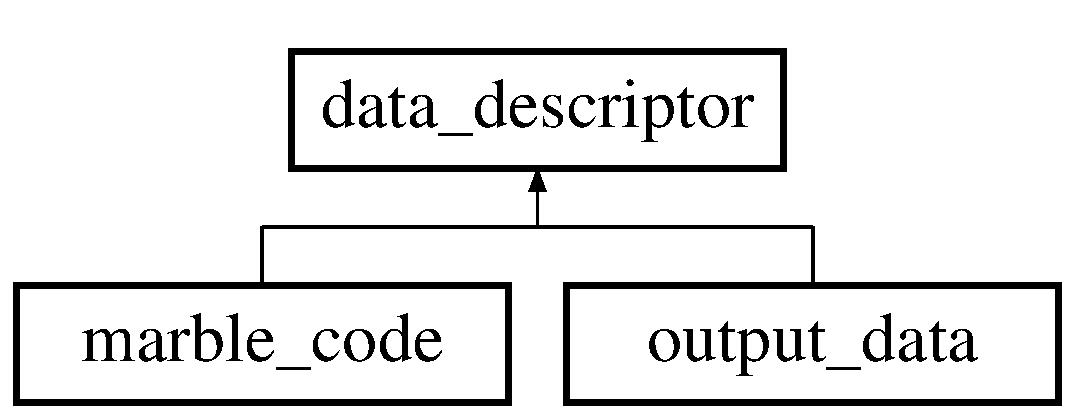
\includegraphics[height=2.000000cm]{structdata__descriptor}
\end{center}
\end{figure}
\subsection*{Public Member Functions}
\begin{DoxyCompactItemize}
\item 
\hyperlink{structdata__descriptor_a6d9ca56cc8c9dc991da573b4de28a24f}{data\+\_\+descriptor} ()
\item 
virtual void \hyperlink{structdata__descriptor_ad6cd92beb7d2b9291e0d130a24faa380}{update} ()
\end{DoxyCompactItemize}
\subsection*{Public Attributes}
\begin{DoxyCompactItemize}
\item 
int \hyperlink{structdata__descriptor_a4a00d6d056ecfcfe90fbcd3df6687e40}{start}
\item 
int \hyperlink{structdata__descriptor_a13601b4b047a84f9ae3b039e1ac7b32f}{end}
\item 
int \hyperlink{structdata__descriptor_a8020a1ab93f8785b3c291794ff9fe072}{size}
\item 
const char $\ast$ \hyperlink{structdata__descriptor_a438b90d9b79eaa4d589d13edc66809cb}{data}
\item 
struct \hyperlink{structsplit}{split} $\ast$ \hyperlink{structdata__descriptor_aae971f7bfb2cd98392b69af23c2245b2}{split}
\end{DoxyCompactItemize}


\subsection{Constructor \& Destructor Documentation}
\mbox{\Hypertarget{structdata__descriptor_a6d9ca56cc8c9dc991da573b4de28a24f}\label{structdata__descriptor_a6d9ca56cc8c9dc991da573b4de28a24f}} 
\index{data\+\_\+descriptor@{data\+\_\+descriptor}!data\+\_\+descriptor@{data\+\_\+descriptor}}
\index{data\+\_\+descriptor@{data\+\_\+descriptor}!data\+\_\+descriptor@{data\+\_\+descriptor}}
\subsubsection{\texorpdfstring{data\+\_\+descriptor()}{data\_descriptor()}}
{\footnotesize\ttfamily data\+\_\+descriptor\+::data\+\_\+descriptor (\begin{DoxyParamCaption}{ }\end{DoxyParamCaption})}



\subsection{Member Function Documentation}
\mbox{\Hypertarget{structdata__descriptor_ad6cd92beb7d2b9291e0d130a24faa380}\label{structdata__descriptor_ad6cd92beb7d2b9291e0d130a24faa380}} 
\index{data\+\_\+descriptor@{data\+\_\+descriptor}!update@{update}}
\index{update@{update}!data\+\_\+descriptor@{data\+\_\+descriptor}}
\subsubsection{\texorpdfstring{update()}{update()}}
{\footnotesize\ttfamily virtual void data\+\_\+descriptor\+::update (\begin{DoxyParamCaption}{ }\end{DoxyParamCaption})\hspace{0.3cm}{\ttfamily [virtual]}}



Reimplemented in \hyperlink{structmarble__code_ac2d593b81e3f340f11e8fe6b8978163b}{marble\+\_\+code}, and \hyperlink{structoutput__data_ad3dd0b4e74cd55dee641af403690ed64}{output\+\_\+data}.



\subsection{Member Data Documentation}
\mbox{\Hypertarget{structdata__descriptor_a438b90d9b79eaa4d589d13edc66809cb}\label{structdata__descriptor_a438b90d9b79eaa4d589d13edc66809cb}} 
\index{data\+\_\+descriptor@{data\+\_\+descriptor}!data@{data}}
\index{data@{data}!data\+\_\+descriptor@{data\+\_\+descriptor}}
\subsubsection{\texorpdfstring{data}{data}}
{\footnotesize\ttfamily const char$\ast$ data\+\_\+descriptor\+::data}

\mbox{\Hypertarget{structdata__descriptor_a13601b4b047a84f9ae3b039e1ac7b32f}\label{structdata__descriptor_a13601b4b047a84f9ae3b039e1ac7b32f}} 
\index{data\+\_\+descriptor@{data\+\_\+descriptor}!end@{end}}
\index{end@{end}!data\+\_\+descriptor@{data\+\_\+descriptor}}
\subsubsection{\texorpdfstring{end}{end}}
{\footnotesize\ttfamily int data\+\_\+descriptor\+::end}

\mbox{\Hypertarget{structdata__descriptor_a8020a1ab93f8785b3c291794ff9fe072}\label{structdata__descriptor_a8020a1ab93f8785b3c291794ff9fe072}} 
\index{data\+\_\+descriptor@{data\+\_\+descriptor}!size@{size}}
\index{size@{size}!data\+\_\+descriptor@{data\+\_\+descriptor}}
\subsubsection{\texorpdfstring{size}{size}}
{\footnotesize\ttfamily int data\+\_\+descriptor\+::size}

\mbox{\Hypertarget{structdata__descriptor_aae971f7bfb2cd98392b69af23c2245b2}\label{structdata__descriptor_aae971f7bfb2cd98392b69af23c2245b2}} 
\index{data\+\_\+descriptor@{data\+\_\+descriptor}!split@{split}}
\index{split@{split}!data\+\_\+descriptor@{data\+\_\+descriptor}}
\subsubsection{\texorpdfstring{split}{split}}
{\footnotesize\ttfamily struct \hyperlink{structsplit}{split}$\ast$ data\+\_\+descriptor\+::split}

\mbox{\Hypertarget{structdata__descriptor_a4a00d6d056ecfcfe90fbcd3df6687e40}\label{structdata__descriptor_a4a00d6d056ecfcfe90fbcd3df6687e40}} 
\index{data\+\_\+descriptor@{data\+\_\+descriptor}!start@{start}}
\index{start@{start}!data\+\_\+descriptor@{data\+\_\+descriptor}}
\subsubsection{\texorpdfstring{start}{start}}
{\footnotesize\ttfamily int data\+\_\+descriptor\+::start}



The documentation for this struct was generated from the following file\+:\begin{DoxyCompactItemize}
\item 
include/\hyperlink{splitter_8h}{splitter.\+h}\end{DoxyCompactItemize}

\hypertarget{classDataType}{}\section{Data\+Type Class Reference}
\label{classDataType}\index{Data\+Type@{Data\+Type}}


{\ttfamily \#include $<$datatype.\+h$>$}

\subsection*{Static Public Member Functions}
\begin{DoxyCompactItemize}
\item 
static bool \hyperlink{classDataType_a8dd169d383b0504b38649fe8ec60352e}{is\+Primitive\+Data\+Type} (std\+::string value)
\end{DoxyCompactItemize}


\subsection{Member Function Documentation}
\mbox{\Hypertarget{classDataType_a8dd169d383b0504b38649fe8ec60352e}\label{classDataType_a8dd169d383b0504b38649fe8ec60352e}} 
\index{Data\+Type@{Data\+Type}!is\+Primitive\+Data\+Type@{is\+Primitive\+Data\+Type}}
\index{is\+Primitive\+Data\+Type@{is\+Primitive\+Data\+Type}!Data\+Type@{Data\+Type}}
\subsubsection{\texorpdfstring{is\+Primitive\+Data\+Type()}{isPrimitiveDataType()}}
{\footnotesize\ttfamily static bool Data\+Type\+::is\+Primitive\+Data\+Type (\begin{DoxyParamCaption}\item[{std\+::string}]{value }\end{DoxyParamCaption})\hspace{0.3cm}{\ttfamily [static]}}



The documentation for this class was generated from the following file\+:\begin{DoxyCompactItemize}
\item 
include/\hyperlink{datatype_8h}{datatype.\+h}\end{DoxyCompactItemize}

\hypertarget{classDebug}{}\section{Debug Class Reference}
\label{classDebug}\index{Debug@{Debug}}


{\ttfamily \#include $<$debug.\+h$>$}

\subsection*{Public Member Functions}
\begin{DoxyCompactItemize}
\item 
\hyperlink{classDebug_a5b453c195c4cfffed2702c3330f53a64}{Debug} ()
\item 
virtual \hyperlink{classDebug_a1effbd1502e249f80a3122b4bdfa7223}{$\sim$\+Debug} ()
\end{DoxyCompactItemize}
\subsection*{Static Public Member Functions}
\begin{DoxyCompactItemize}
\item 
static void \hyperlink{classDebug_ae57630ccc6a2e3807f698ed6fef69786}{Output\+Tabbing} (int amount)
\item 
static void \hyperlink{classDebug_a104d2378a5e251c0b4fb4fdb58802ead}{Print\+Value\+For\+Node} (\hyperlink{classNode}{Node} $\ast$value\+\_\+node, int tabbing=0)
\end{DoxyCompactItemize}


\subsection{Constructor \& Destructor Documentation}
\mbox{\Hypertarget{classDebug_a5b453c195c4cfffed2702c3330f53a64}\label{classDebug_a5b453c195c4cfffed2702c3330f53a64}} 
\index{Debug@{Debug}!Debug@{Debug}}
\index{Debug@{Debug}!Debug@{Debug}}
\subsubsection{\texorpdfstring{Debug()}{Debug()}}
{\footnotesize\ttfamily Debug\+::\+Debug (\begin{DoxyParamCaption}{ }\end{DoxyParamCaption})}

\mbox{\Hypertarget{classDebug_a1effbd1502e249f80a3122b4bdfa7223}\label{classDebug_a1effbd1502e249f80a3122b4bdfa7223}} 
\index{Debug@{Debug}!````~Debug@{$\sim$\+Debug}}
\index{````~Debug@{$\sim$\+Debug}!Debug@{Debug}}
\subsubsection{\texorpdfstring{$\sim$\+Debug()}{~Debug()}}
{\footnotesize\ttfamily virtual Debug\+::$\sim$\+Debug (\begin{DoxyParamCaption}{ }\end{DoxyParamCaption})\hspace{0.3cm}{\ttfamily [virtual]}}



\subsection{Member Function Documentation}
\mbox{\Hypertarget{classDebug_ae57630ccc6a2e3807f698ed6fef69786}\label{classDebug_ae57630ccc6a2e3807f698ed6fef69786}} 
\index{Debug@{Debug}!Output\+Tabbing@{Output\+Tabbing}}
\index{Output\+Tabbing@{Output\+Tabbing}!Debug@{Debug}}
\subsubsection{\texorpdfstring{Output\+Tabbing()}{OutputTabbing()}}
{\footnotesize\ttfamily static void Debug\+::\+Output\+Tabbing (\begin{DoxyParamCaption}\item[{int}]{amount }\end{DoxyParamCaption})\hspace{0.3cm}{\ttfamily [static]}}

\mbox{\Hypertarget{classDebug_a104d2378a5e251c0b4fb4fdb58802ead}\label{classDebug_a104d2378a5e251c0b4fb4fdb58802ead}} 
\index{Debug@{Debug}!Print\+Value\+For\+Node@{Print\+Value\+For\+Node}}
\index{Print\+Value\+For\+Node@{Print\+Value\+For\+Node}!Debug@{Debug}}
\subsubsection{\texorpdfstring{Print\+Value\+For\+Node()}{PrintValueForNode()}}
{\footnotesize\ttfamily static void Debug\+::\+Print\+Value\+For\+Node (\begin{DoxyParamCaption}\item[{\hyperlink{classNode}{Node} $\ast$}]{value\+\_\+node,  }\item[{int}]{tabbing = {\ttfamily 0} }\end{DoxyParamCaption})\hspace{0.3cm}{\ttfamily [static]}}



The documentation for this class was generated from the following file\+:\begin{DoxyCompactItemize}
\item 
include/\hyperlink{debug_8h}{debug.\+h}\end{DoxyCompactItemize}

\hypertarget{classEvaluatingNode}{}\section{Evaluating\+Node Class Reference}
\label{classEvaluatingNode}\index{Evaluating\+Node@{Evaluating\+Node}}


{\ttfamily \#include $<$evaluatingnode.\+h$>$}

Inheritance diagram for Evaluating\+Node\+:\begin{figure}[H]
\begin{center}
\leavevmode
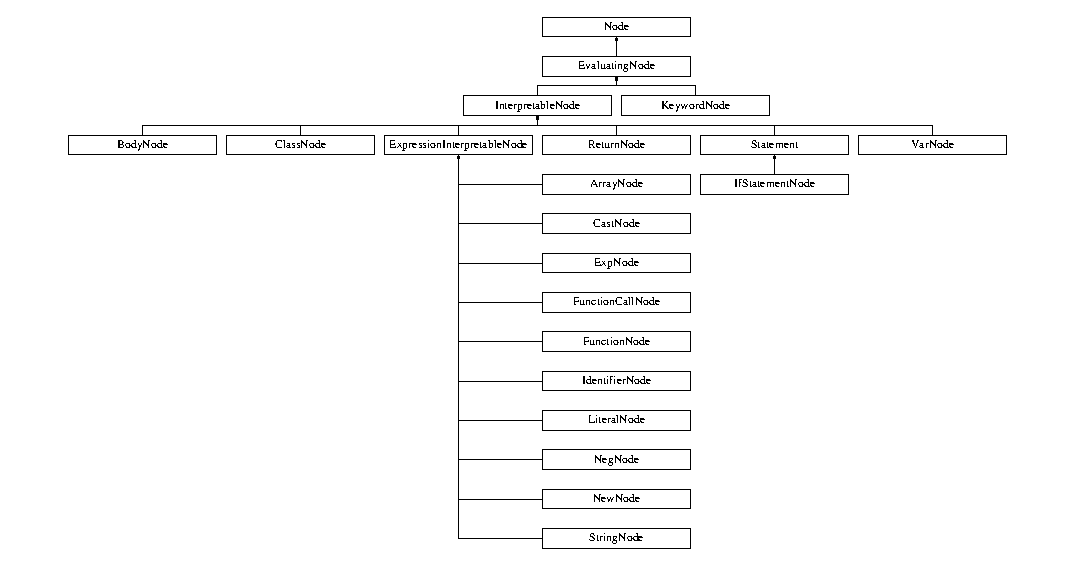
\includegraphics[height=7.140255cm]{classEvaluatingNode}
\end{center}
\end{figure}
\subsection*{Public Member Functions}
\begin{DoxyCompactItemize}
\item 
\hyperlink{classEvaluatingNode_a0ece59961a22a6f07d53e75f41707683}{Evaluating\+Node} (\hyperlink{statics_8h_a1ec6d4bfce2e004debbc141eafc512db}{N\+O\+D\+E\+\_\+\+T\+Y\+PE} \hyperlink{classNode_af4f536b1b3f60e197fe364ba56022291}{type})
\item 
virtual \hyperlink{classEvaluatingNode_aac142cb781f91833f01c537f3b76b1d2}{$\sim$\+Evaluating\+Node} ()
\item 
struct \hyperlink{structEvaluation}{Evaluation} \hyperlink{classEvaluatingNode_a49e3ccc15a4fc2d4ecd4d264c86dea5e}{evaluate} (\hyperlink{classSystemHandler}{System\+Handler} $\ast$handler, \hyperlink{statics_8h_a6664c451ca7787483a7981cc1de68dbb}{E\+V\+A\+L\+U\+A\+T\+I\+O\+N\+\_\+\+T\+Y\+PE} expected\+\_\+evaluation)
\item 
void \hyperlink{classEvaluatingNode_ae20449b7c2e423d64664503befd47ba0}{evaluate} (\hyperlink{classSystemHandler}{System\+Handler} $\ast$handler, \hyperlink{statics_8h_a6664c451ca7787483a7981cc1de68dbb}{E\+V\+A\+L\+U\+A\+T\+I\+O\+N\+\_\+\+T\+Y\+PE} expected\+\_\+evaluation, struct \hyperlink{structEvaluation}{Evaluation} $\ast$evaluation)
\end{DoxyCompactItemize}
\subsection*{Protected Member Functions}
\begin{DoxyCompactItemize}
\item 
virtual void \hyperlink{classEvaluatingNode_a085fa06e0b46a93c814dc55cda0c1b26}{evaluate\+\_\+impl} (\hyperlink{classSystemHandler}{System\+Handler} $\ast$handler, \hyperlink{statics_8h_a6664c451ca7787483a7981cc1de68dbb}{E\+V\+A\+L\+U\+A\+T\+I\+O\+N\+\_\+\+T\+Y\+PE} expected\+\_\+evaluation, struct \hyperlink{structEvaluation}{Evaluation} $\ast$evaluation)=0
\end{DoxyCompactItemize}
\subsection*{Additional Inherited Members}


\subsection{Constructor \& Destructor Documentation}
\mbox{\Hypertarget{classEvaluatingNode_a0ece59961a22a6f07d53e75f41707683}\label{classEvaluatingNode_a0ece59961a22a6f07d53e75f41707683}} 
\index{Evaluating\+Node@{Evaluating\+Node}!Evaluating\+Node@{Evaluating\+Node}}
\index{Evaluating\+Node@{Evaluating\+Node}!Evaluating\+Node@{Evaluating\+Node}}
\subsubsection{\texorpdfstring{Evaluating\+Node()}{EvaluatingNode()}}
{\footnotesize\ttfamily Evaluating\+Node\+::\+Evaluating\+Node (\begin{DoxyParamCaption}\item[{\hyperlink{statics_8h_a1ec6d4bfce2e004debbc141eafc512db}{N\+O\+D\+E\+\_\+\+T\+Y\+PE}}]{type }\end{DoxyParamCaption})}

\mbox{\Hypertarget{classEvaluatingNode_aac142cb781f91833f01c537f3b76b1d2}\label{classEvaluatingNode_aac142cb781f91833f01c537f3b76b1d2}} 
\index{Evaluating\+Node@{Evaluating\+Node}!````~Evaluating\+Node@{$\sim$\+Evaluating\+Node}}
\index{````~Evaluating\+Node@{$\sim$\+Evaluating\+Node}!Evaluating\+Node@{Evaluating\+Node}}
\subsubsection{\texorpdfstring{$\sim$\+Evaluating\+Node()}{~EvaluatingNode()}}
{\footnotesize\ttfamily virtual Evaluating\+Node\+::$\sim$\+Evaluating\+Node (\begin{DoxyParamCaption}{ }\end{DoxyParamCaption})\hspace{0.3cm}{\ttfamily [virtual]}}



\subsection{Member Function Documentation}
\mbox{\Hypertarget{classEvaluatingNode_a49e3ccc15a4fc2d4ecd4d264c86dea5e}\label{classEvaluatingNode_a49e3ccc15a4fc2d4ecd4d264c86dea5e}} 
\index{Evaluating\+Node@{Evaluating\+Node}!evaluate@{evaluate}}
\index{evaluate@{evaluate}!Evaluating\+Node@{Evaluating\+Node}}
\subsubsection{\texorpdfstring{evaluate()}{evaluate()}\hspace{0.1cm}{\footnotesize\ttfamily [1/2]}}
{\footnotesize\ttfamily struct \hyperlink{structEvaluation}{Evaluation} Evaluating\+Node\+::evaluate (\begin{DoxyParamCaption}\item[{\hyperlink{classSystemHandler}{System\+Handler} $\ast$}]{handler,  }\item[{\hyperlink{statics_8h_a6664c451ca7787483a7981cc1de68dbb}{E\+V\+A\+L\+U\+A\+T\+I\+O\+N\+\_\+\+T\+Y\+PE}}]{expected\+\_\+evaluation }\end{DoxyParamCaption})}

\mbox{\Hypertarget{classEvaluatingNode_ae20449b7c2e423d64664503befd47ba0}\label{classEvaluatingNode_ae20449b7c2e423d64664503befd47ba0}} 
\index{Evaluating\+Node@{Evaluating\+Node}!evaluate@{evaluate}}
\index{evaluate@{evaluate}!Evaluating\+Node@{Evaluating\+Node}}
\subsubsection{\texorpdfstring{evaluate()}{evaluate()}\hspace{0.1cm}{\footnotesize\ttfamily [2/2]}}
{\footnotesize\ttfamily void Evaluating\+Node\+::evaluate (\begin{DoxyParamCaption}\item[{\hyperlink{classSystemHandler}{System\+Handler} $\ast$}]{handler,  }\item[{\hyperlink{statics_8h_a6664c451ca7787483a7981cc1de68dbb}{E\+V\+A\+L\+U\+A\+T\+I\+O\+N\+\_\+\+T\+Y\+PE}}]{expected\+\_\+evaluation,  }\item[{struct \hyperlink{structEvaluation}{Evaluation} $\ast$}]{evaluation }\end{DoxyParamCaption})}

\mbox{\Hypertarget{classEvaluatingNode_a085fa06e0b46a93c814dc55cda0c1b26}\label{classEvaluatingNode_a085fa06e0b46a93c814dc55cda0c1b26}} 
\index{Evaluating\+Node@{Evaluating\+Node}!evaluate\+\_\+impl@{evaluate\+\_\+impl}}
\index{evaluate\+\_\+impl@{evaluate\+\_\+impl}!Evaluating\+Node@{Evaluating\+Node}}
\subsubsection{\texorpdfstring{evaluate\+\_\+impl()}{evaluate\_impl()}}
{\footnotesize\ttfamily virtual void Evaluating\+Node\+::evaluate\+\_\+impl (\begin{DoxyParamCaption}\item[{\hyperlink{classSystemHandler}{System\+Handler} $\ast$}]{handler,  }\item[{\hyperlink{statics_8h_a6664c451ca7787483a7981cc1de68dbb}{E\+V\+A\+L\+U\+A\+T\+I\+O\+N\+\_\+\+T\+Y\+PE}}]{expected\+\_\+evaluation,  }\item[{struct \hyperlink{structEvaluation}{Evaluation} $\ast$}]{evaluation }\end{DoxyParamCaption})\hspace{0.3cm}{\ttfamily [protected]}, {\ttfamily [pure virtual]}}



Implemented in \hyperlink{classExpNode_a58c05ac75051f109512ce8fa5ceb68c7}{Exp\+Node}, \hyperlink{classNewNode_a53fe843af3bbb2add900646ef3891f8e}{New\+Node}, \hyperlink{classVarNode_affe926e80803de0a83ce88f9a0d97db3}{Var\+Node}, \hyperlink{classFunctionCallNode_a65f15b75804343caf5c4ce291460b1dc}{Function\+Call\+Node}, \hyperlink{classFunctionNode_a697f1fdc368f5ad09284b32b4466f353}{Function\+Node}, \hyperlink{classBodyNode_ab08c6586b725065afca095786b842991}{Body\+Node}, \hyperlink{classCastNode_ae0c32d5d076c2572fa7afc9cb1a76a79}{Cast\+Node}, \hyperlink{classLiteralNode_ac468128f093b3955ddd7c85eaa959ec2}{Literal\+Node}, \hyperlink{classArrayNode_aeefbfe735ed37a81785a492dbc66eddc}{Array\+Node}, \hyperlink{classClassNode_ab969f53cd181de184a8f82273dbd77ab}{Class\+Node}, \hyperlink{classIdentifierNode_a4960a1e68623066e413f8c2d68cee7e5}{Identifier\+Node}, \hyperlink{classKeywordNode_a699f7171c8415901b1a501f72933cfdf}{Keyword\+Node}, \hyperlink{classNegNode_a504b9103413ac571d7a332cd4dd0b9c5}{Neg\+Node}, \hyperlink{classStringNode_a1399a24e093f4ecd00957268923c5d23}{String\+Node}, \hyperlink{classIfStatementNode_a725287a819ddcdc914cf774da80272e4}{If\+Statement\+Node}, and \hyperlink{classReturnNode_ac07545808632b52ec192cce2dd80b051}{Return\+Node}.



The documentation for this class was generated from the following file\+:\begin{DoxyCompactItemize}
\item 
include/\hyperlink{evaluatingnode_8h}{evaluatingnode.\+h}\end{DoxyCompactItemize}

\hypertarget{structEvaluation}{}\section{Evaluation Struct Reference}
\label{structEvaluation}\index{Evaluation@{Evaluation}}


{\ttfamily \#include $<$evaluatingnode.\+h$>$}

\subsection*{Classes}
\begin{DoxyCompactItemize}
\item 
struct \hyperlink{structEvaluation_1_1datatype}{datatype}
\end{DoxyCompactItemize}
\subsection*{Public Attributes}
\begin{DoxyCompactItemize}
\item 
\hyperlink{statics_8h_a6664c451ca7787483a7981cc1de68dbb}{E\+V\+A\+L\+U\+A\+T\+I\+O\+N\+\_\+\+T\+Y\+PE} \hyperlink{structEvaluation_ab056e930fde1d7f4ce8474e31f133860}{type} = 0
\item 
struct \hyperlink{structEvaluation_1_1datatype}{Evaluation\+::datatype} \hyperlink{structEvaluation_afd26f89d96c69704172ddcce5d08fee4}{datatype}
\end{DoxyCompactItemize}


\subsection{Member Data Documentation}
\mbox{\Hypertarget{structEvaluation_afd26f89d96c69704172ddcce5d08fee4}\label{structEvaluation_afd26f89d96c69704172ddcce5d08fee4}} 
\index{Evaluation@{Evaluation}!datatype@{datatype}}
\index{datatype@{datatype}!Evaluation@{Evaluation}}
\subsubsection{\texorpdfstring{datatype}{datatype}}
{\footnotesize\ttfamily struct \hyperlink{structEvaluation_1_1datatype}{Evaluation\+::datatype}  \hyperlink{structEvaluation_1_1datatype}{Evaluation\+::datatype}}

\mbox{\Hypertarget{structEvaluation_ab056e930fde1d7f4ce8474e31f133860}\label{structEvaluation_ab056e930fde1d7f4ce8474e31f133860}} 
\index{Evaluation@{Evaluation}!type@{type}}
\index{type@{type}!Evaluation@{Evaluation}}
\subsubsection{\texorpdfstring{type}{type}}
{\footnotesize\ttfamily \hyperlink{statics_8h_a6664c451ca7787483a7981cc1de68dbb}{E\+V\+A\+L\+U\+A\+T\+I\+O\+N\+\_\+\+T\+Y\+PE} Evaluation\+::type = 0}



The documentation for this struct was generated from the following file\+:\begin{DoxyCompactItemize}
\item 
include/\hyperlink{evaluatingnode_8h}{evaluatingnode.\+h}\end{DoxyCompactItemize}

\hypertarget{classExpNode}{}\section{Exp\+Node Class Reference}
\label{classExpNode}\index{Exp\+Node@{Exp\+Node}}


{\ttfamily \#include $<$expnode.\+h$>$}

Inheritance diagram for Exp\+Node\+:\begin{figure}[H]
\begin{center}
\leavevmode
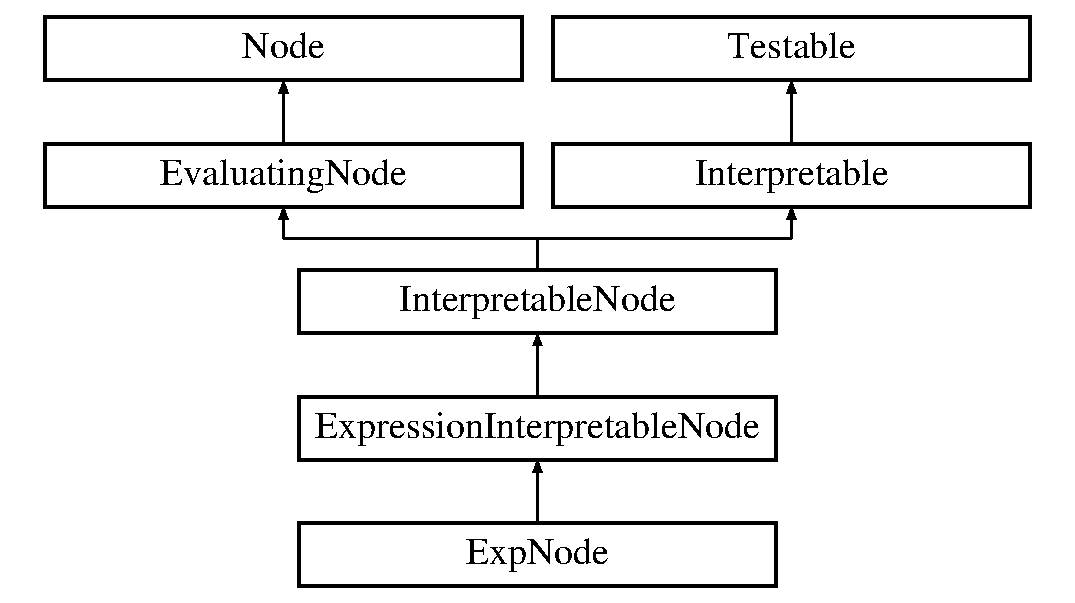
\includegraphics[height=5.000000cm]{classExpNode}
\end{center}
\end{figure}
\subsection*{Public Member Functions}
\begin{DoxyCompactItemize}
\item 
\hyperlink{classExpNode_a72dae84bdb441ca58d862a36912a5f67}{Exp\+Node} ()
\item 
virtual \hyperlink{classExpNode_a217540657865f605cb6847280e00bb21}{$\sim$\+Exp\+Node} ()
\item 
virtual \hyperlink{classValue}{Value} \hyperlink{classExpNode_aedff3b19b9e36a77e4558a168b81debf}{interpret} (\hyperlink{classInterpreter}{Interpreter} $\ast$intrerpreter)
\item 
virtual void \hyperlink{classExpNode_a8fb8302d5ce438a9ad0f58161be2a1c9}{test} (\hyperlink{classValidator}{Validator} $\ast$validator)
\item 
void \hyperlink{classExpNode_a84953d6f8662cdbcbe84aeb875d87939}{test\+\_\+obj\+\_\+access} (\hyperlink{classValidator}{Validator} $\ast$validator)
\item 
void \hyperlink{classExpNode_aac9d0df6bb5cae7d98a085269cf47937}{test\+\_\+assign} (\hyperlink{classValidator}{Validator} $\ast$validator)
\item 
void \hyperlink{classExpNode_ab5fbb36f2d6beebe5cd5c9a651debc57}{test\+\_\+regular\+\_\+exp} (\hyperlink{classValidator}{Validator} $\ast$validator)
\item 
virtual void \hyperlink{classExpNode_a58c05ac75051f109512ce8fa5ceb68c7}{evaluate\+\_\+impl} (\hyperlink{classSystemHandler}{System\+Handler} $\ast$handler, \hyperlink{statics_8h_a6664c451ca7787483a7981cc1de68dbb}{E\+V\+A\+L\+U\+A\+T\+I\+O\+N\+\_\+\+T\+Y\+PE} expected\+\_\+evaluation, struct \hyperlink{structEvaluation}{Evaluation} $\ast$evaluation)
\item 
bool \hyperlink{classExpNode_a39851ed23963fe02e427a7c8c4d61739}{is\+Assignment\+Operator} ()
\end{DoxyCompactItemize}
\subsection*{Public Attributes}
\begin{DoxyCompactItemize}
\item 
\hyperlink{classExpressionInterpretableNode}{Expression\+Interpretable\+Node} $\ast$ \hyperlink{classExpNode_abd5f79666f0b8f05e7a3fca1bfc12ebe}{left}
\item 
\hyperlink{classExpressionInterpretableNode}{Expression\+Interpretable\+Node} $\ast$ \hyperlink{classExpNode_af298caffdc70c8f20095af1191e801cd}{right}
\item 
std\+::string \hyperlink{classExpNode_a7ad8830c081f08f598e4697539b22c28}{op}
\end{DoxyCompactItemize}
\subsection*{Additional Inherited Members}


\subsection{Constructor \& Destructor Documentation}
\mbox{\Hypertarget{classExpNode_a72dae84bdb441ca58d862a36912a5f67}\label{classExpNode_a72dae84bdb441ca58d862a36912a5f67}} 
\index{Exp\+Node@{Exp\+Node}!Exp\+Node@{Exp\+Node}}
\index{Exp\+Node@{Exp\+Node}!Exp\+Node@{Exp\+Node}}
\subsubsection{\texorpdfstring{Exp\+Node()}{ExpNode()}}
{\footnotesize\ttfamily Exp\+Node\+::\+Exp\+Node (\begin{DoxyParamCaption}{ }\end{DoxyParamCaption})}

\mbox{\Hypertarget{classExpNode_a217540657865f605cb6847280e00bb21}\label{classExpNode_a217540657865f605cb6847280e00bb21}} 
\index{Exp\+Node@{Exp\+Node}!````~Exp\+Node@{$\sim$\+Exp\+Node}}
\index{````~Exp\+Node@{$\sim$\+Exp\+Node}!Exp\+Node@{Exp\+Node}}
\subsubsection{\texorpdfstring{$\sim$\+Exp\+Node()}{~ExpNode()}}
{\footnotesize\ttfamily virtual Exp\+Node\+::$\sim$\+Exp\+Node (\begin{DoxyParamCaption}{ }\end{DoxyParamCaption})\hspace{0.3cm}{\ttfamily [virtual]}}



\subsection{Member Function Documentation}
\mbox{\Hypertarget{classExpNode_a58c05ac75051f109512ce8fa5ceb68c7}\label{classExpNode_a58c05ac75051f109512ce8fa5ceb68c7}} 
\index{Exp\+Node@{Exp\+Node}!evaluate\+\_\+impl@{evaluate\+\_\+impl}}
\index{evaluate\+\_\+impl@{evaluate\+\_\+impl}!Exp\+Node@{Exp\+Node}}
\subsubsection{\texorpdfstring{evaluate\+\_\+impl()}{evaluate\_impl()}}
{\footnotesize\ttfamily virtual void Exp\+Node\+::evaluate\+\_\+impl (\begin{DoxyParamCaption}\item[{\hyperlink{classSystemHandler}{System\+Handler} $\ast$}]{handler,  }\item[{\hyperlink{statics_8h_a6664c451ca7787483a7981cc1de68dbb}{E\+V\+A\+L\+U\+A\+T\+I\+O\+N\+\_\+\+T\+Y\+PE}}]{expected\+\_\+evaluation,  }\item[{struct \hyperlink{structEvaluation}{Evaluation} $\ast$}]{evaluation }\end{DoxyParamCaption})\hspace{0.3cm}{\ttfamily [virtual]}}



Reimplemented from \hyperlink{classEvaluatingNode_abb86fa7334a5871f959b0633db3b5215}{Evaluating\+Node}.

\mbox{\Hypertarget{classExpNode_aedff3b19b9e36a77e4558a168b81debf}\label{classExpNode_aedff3b19b9e36a77e4558a168b81debf}} 
\index{Exp\+Node@{Exp\+Node}!interpret@{interpret}}
\index{interpret@{interpret}!Exp\+Node@{Exp\+Node}}
\subsubsection{\texorpdfstring{interpret()}{interpret()}}
{\footnotesize\ttfamily virtual \hyperlink{classValue}{Value} Exp\+Node\+::interpret (\begin{DoxyParamCaption}\item[{\hyperlink{classInterpreter}{Interpreter} $\ast$}]{intrerpreter }\end{DoxyParamCaption})\hspace{0.3cm}{\ttfamily [virtual]}}



Implements \hyperlink{classExpressionInterpretableNode_a43650f046c48fc539f77a207e3c9181e}{Expression\+Interpretable\+Node}.

\mbox{\Hypertarget{classExpNode_a39851ed23963fe02e427a7c8c4d61739}\label{classExpNode_a39851ed23963fe02e427a7c8c4d61739}} 
\index{Exp\+Node@{Exp\+Node}!is\+Assignment\+Operator@{is\+Assignment\+Operator}}
\index{is\+Assignment\+Operator@{is\+Assignment\+Operator}!Exp\+Node@{Exp\+Node}}
\subsubsection{\texorpdfstring{is\+Assignment\+Operator()}{isAssignmentOperator()}}
{\footnotesize\ttfamily bool Exp\+Node\+::is\+Assignment\+Operator (\begin{DoxyParamCaption}{ }\end{DoxyParamCaption})}

\mbox{\Hypertarget{classExpNode_a8fb8302d5ce438a9ad0f58161be2a1c9}\label{classExpNode_a8fb8302d5ce438a9ad0f58161be2a1c9}} 
\index{Exp\+Node@{Exp\+Node}!test@{test}}
\index{test@{test}!Exp\+Node@{Exp\+Node}}
\subsubsection{\texorpdfstring{test()}{test()}}
{\footnotesize\ttfamily virtual void Exp\+Node\+::test (\begin{DoxyParamCaption}\item[{\hyperlink{classValidator}{Validator} $\ast$}]{validator }\end{DoxyParamCaption})\hspace{0.3cm}{\ttfamily [virtual]}}



Reimplemented from \hyperlink{classInterpretable_a32f547aaf68dcbab993284d3257ab010}{Interpretable}.

\mbox{\Hypertarget{classExpNode_aac9d0df6bb5cae7d98a085269cf47937}\label{classExpNode_aac9d0df6bb5cae7d98a085269cf47937}} 
\index{Exp\+Node@{Exp\+Node}!test\+\_\+assign@{test\+\_\+assign}}
\index{test\+\_\+assign@{test\+\_\+assign}!Exp\+Node@{Exp\+Node}}
\subsubsection{\texorpdfstring{test\+\_\+assign()}{test\_assign()}}
{\footnotesize\ttfamily void Exp\+Node\+::test\+\_\+assign (\begin{DoxyParamCaption}\item[{\hyperlink{classValidator}{Validator} $\ast$}]{validator }\end{DoxyParamCaption})}

\mbox{\Hypertarget{classExpNode_a84953d6f8662cdbcbe84aeb875d87939}\label{classExpNode_a84953d6f8662cdbcbe84aeb875d87939}} 
\index{Exp\+Node@{Exp\+Node}!test\+\_\+obj\+\_\+access@{test\+\_\+obj\+\_\+access}}
\index{test\+\_\+obj\+\_\+access@{test\+\_\+obj\+\_\+access}!Exp\+Node@{Exp\+Node}}
\subsubsection{\texorpdfstring{test\+\_\+obj\+\_\+access()}{test\_obj\_access()}}
{\footnotesize\ttfamily void Exp\+Node\+::test\+\_\+obj\+\_\+access (\begin{DoxyParamCaption}\item[{\hyperlink{classValidator}{Validator} $\ast$}]{validator }\end{DoxyParamCaption})}

\mbox{\Hypertarget{classExpNode_ab5fbb36f2d6beebe5cd5c9a651debc57}\label{classExpNode_ab5fbb36f2d6beebe5cd5c9a651debc57}} 
\index{Exp\+Node@{Exp\+Node}!test\+\_\+regular\+\_\+exp@{test\+\_\+regular\+\_\+exp}}
\index{test\+\_\+regular\+\_\+exp@{test\+\_\+regular\+\_\+exp}!Exp\+Node@{Exp\+Node}}
\subsubsection{\texorpdfstring{test\+\_\+regular\+\_\+exp()}{test\_regular\_exp()}}
{\footnotesize\ttfamily void Exp\+Node\+::test\+\_\+regular\+\_\+exp (\begin{DoxyParamCaption}\item[{\hyperlink{classValidator}{Validator} $\ast$}]{validator }\end{DoxyParamCaption})}



\subsection{Member Data Documentation}
\mbox{\Hypertarget{classExpNode_abd5f79666f0b8f05e7a3fca1bfc12ebe}\label{classExpNode_abd5f79666f0b8f05e7a3fca1bfc12ebe}} 
\index{Exp\+Node@{Exp\+Node}!left@{left}}
\index{left@{left}!Exp\+Node@{Exp\+Node}}
\subsubsection{\texorpdfstring{left}{left}}
{\footnotesize\ttfamily \hyperlink{classExpressionInterpretableNode}{Expression\+Interpretable\+Node}$\ast$ Exp\+Node\+::left}

\mbox{\Hypertarget{classExpNode_a7ad8830c081f08f598e4697539b22c28}\label{classExpNode_a7ad8830c081f08f598e4697539b22c28}} 
\index{Exp\+Node@{Exp\+Node}!op@{op}}
\index{op@{op}!Exp\+Node@{Exp\+Node}}
\subsubsection{\texorpdfstring{op}{op}}
{\footnotesize\ttfamily std\+::string Exp\+Node\+::op}

\mbox{\Hypertarget{classExpNode_af298caffdc70c8f20095af1191e801cd}\label{classExpNode_af298caffdc70c8f20095af1191e801cd}} 
\index{Exp\+Node@{Exp\+Node}!right@{right}}
\index{right@{right}!Exp\+Node@{Exp\+Node}}
\subsubsection{\texorpdfstring{right}{right}}
{\footnotesize\ttfamily \hyperlink{classExpressionInterpretableNode}{Expression\+Interpretable\+Node}$\ast$ Exp\+Node\+::right}



The documentation for this class was generated from the following file\+:\begin{DoxyCompactItemize}
\item 
include/\hyperlink{expnode_8h}{expnode.\+h}\end{DoxyCompactItemize}

\hypertarget{classExpressionInterpretableNode}{}\section{Expression\+Interpretable\+Node Class Reference}
\label{classExpressionInterpretableNode}\index{Expression\+Interpretable\+Node@{Expression\+Interpretable\+Node}}


{\ttfamily \#include $<$einode.\+h$>$}

Inheritance diagram for Expression\+Interpretable\+Node\+:\begin{figure}[H]
\begin{center}
\leavevmode
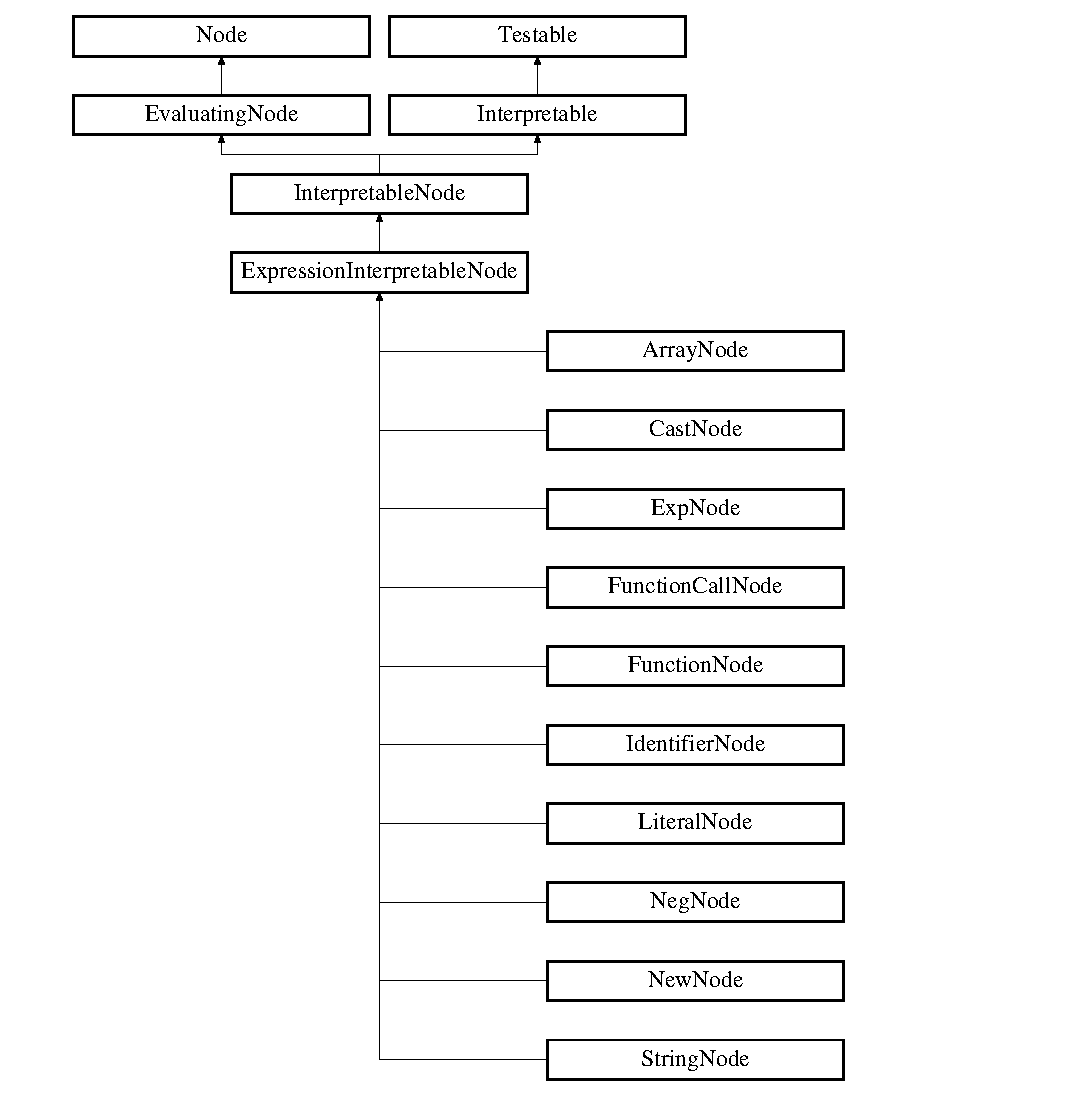
\includegraphics[height=12.000000cm]{classExpressionInterpretableNode}
\end{center}
\end{figure}
\subsection*{Public Member Functions}
\begin{DoxyCompactItemize}
\item 
\hyperlink{classExpressionInterpretableNode_ada38422992af67b30cca93c59bfce188}{Expression\+Interpretable\+Node} (int \hyperlink{classNode_af4f536b1b3f60e197fe364ba56022291}{type})
\item 
virtual \hyperlink{classExpressionInterpretableNode_a3774db564fad38ea68ca0edf235c97aa}{$\sim$\+Expression\+Interpretable\+Node} ()
\item 
virtual \hyperlink{classValue}{Value} \hyperlink{classExpressionInterpretableNode_a43650f046c48fc539f77a207e3c9181e}{interpret} (\hyperlink{classInterpreter}{Interpreter} $\ast$interpreter)=0
\end{DoxyCompactItemize}
\subsection*{Additional Inherited Members}


\subsection{Constructor \& Destructor Documentation}
\mbox{\Hypertarget{classExpressionInterpretableNode_ada38422992af67b30cca93c59bfce188}\label{classExpressionInterpretableNode_ada38422992af67b30cca93c59bfce188}} 
\index{Expression\+Interpretable\+Node@{Expression\+Interpretable\+Node}!Expression\+Interpretable\+Node@{Expression\+Interpretable\+Node}}
\index{Expression\+Interpretable\+Node@{Expression\+Interpretable\+Node}!Expression\+Interpretable\+Node@{Expression\+Interpretable\+Node}}
\subsubsection{\texorpdfstring{Expression\+Interpretable\+Node()}{ExpressionInterpretableNode()}}
{\footnotesize\ttfamily Expression\+Interpretable\+Node\+::\+Expression\+Interpretable\+Node (\begin{DoxyParamCaption}\item[{int}]{type }\end{DoxyParamCaption})}

\mbox{\Hypertarget{classExpressionInterpretableNode_a3774db564fad38ea68ca0edf235c97aa}\label{classExpressionInterpretableNode_a3774db564fad38ea68ca0edf235c97aa}} 
\index{Expression\+Interpretable\+Node@{Expression\+Interpretable\+Node}!````~Expression\+Interpretable\+Node@{$\sim$\+Expression\+Interpretable\+Node}}
\index{````~Expression\+Interpretable\+Node@{$\sim$\+Expression\+Interpretable\+Node}!Expression\+Interpretable\+Node@{Expression\+Interpretable\+Node}}
\subsubsection{\texorpdfstring{$\sim$\+Expression\+Interpretable\+Node()}{~ExpressionInterpretableNode()}}
{\footnotesize\ttfamily virtual Expression\+Interpretable\+Node\+::$\sim$\+Expression\+Interpretable\+Node (\begin{DoxyParamCaption}{ }\end{DoxyParamCaption})\hspace{0.3cm}{\ttfamily [virtual]}}



\subsection{Member Function Documentation}
\mbox{\Hypertarget{classExpressionInterpretableNode_a43650f046c48fc539f77a207e3c9181e}\label{classExpressionInterpretableNode_a43650f046c48fc539f77a207e3c9181e}} 
\index{Expression\+Interpretable\+Node@{Expression\+Interpretable\+Node}!interpret@{interpret}}
\index{interpret@{interpret}!Expression\+Interpretable\+Node@{Expression\+Interpretable\+Node}}
\subsubsection{\texorpdfstring{interpret()}{interpret()}}
{\footnotesize\ttfamily virtual \hyperlink{classValue}{Value} Expression\+Interpretable\+Node\+::interpret (\begin{DoxyParamCaption}\item[{\hyperlink{classInterpreter}{Interpreter} $\ast$}]{interpreter }\end{DoxyParamCaption})\hspace{0.3cm}{\ttfamily [pure virtual]}}



Implements \hyperlink{classInterpretableNode_a9a466e7d65c4b323d2b96b4ac8396cd7}{Interpretable\+Node}.



Implemented in \hyperlink{classNewNode_a77447b9402f0153401bf0e623b5f1e6e}{New\+Node}, \hyperlink{classFunctionCallNode_a1d0d8806b7dd501ed43da58f77f7c49e}{Function\+Call\+Node}, \hyperlink{classFunctionNode_a059e6682cd51d0e126372a7af257ea5a}{Function\+Node}, \hyperlink{classExpNode_aedff3b19b9e36a77e4558a168b81debf}{Exp\+Node}, \hyperlink{classLiteralNode_abb32ed943c6a5b2029a496ac04885b2a}{Literal\+Node}, \hyperlink{classArrayNode_a029220b946233e22cb661fcfac9634d0}{Array\+Node}, \hyperlink{classCastNode_a2a909a7531791bcbc53c514a01ce5024}{Cast\+Node}, \hyperlink{classIdentifierNode_aa7be7da3e018352f8b549fcac3a8155a}{Identifier\+Node}, \hyperlink{classNegNode_a35ff48d55ab355e27f33dcc21483e4c7}{Neg\+Node}, and \hyperlink{classStringNode_ae92c0858cd07baf0c6417f7bdfce9f0d}{String\+Node}.



The documentation for this class was generated from the following file\+:\begin{DoxyCompactItemize}
\item 
include/\hyperlink{einode_8h}{einode.\+h}\end{DoxyCompactItemize}

\hypertarget{classFunction}{}\section{Function Class Reference}
\label{classFunction}\index{Function@{Function}}


{\ttfamily \#include $<$function.\+h$>$}

Inheritance diagram for Function\+:\begin{figure}[H]
\begin{center}
\leavevmode
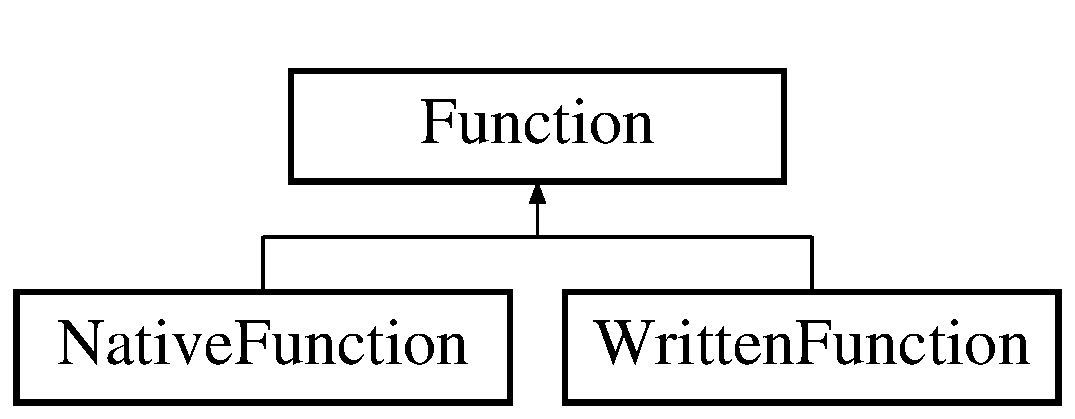
\includegraphics[height=3.000000cm]{classFunction}
\end{center}
\end{figure}
\subsection*{Public Member Functions}
\begin{DoxyCompactItemize}
\item 
\hyperlink{classFunction_a3bcd0502247ea1545853f1f6126b5fe1}{Function} (\hyperlink{statics_8h_a025d9866e39f51183a23b3e2165f0e77}{F\+U\+N\+C\+T\+I\+O\+N\+\_\+\+T\+Y\+PE} \hyperlink{classFunction_a07d7969dbcf44a6a066c6e042a02983d}{type}, std\+::string \hyperlink{classFunction_a161d1ceb4f67f3222caf429fea7b71f1}{name})
\item 
virtual \hyperlink{classFunction_a8697b2e490a4314a7ccbb17aea8ce537}{$\sim$\+Function} ()
\item 
std\+::string \hyperlink{classFunction_a5b7d859d767e8a9c19fc5b81a0d10395}{get\+Name} ()
\item 
virtual void \hyperlink{classFunction_a84f9a63e68becc27e58ea738ba4cd698}{invoke} (std\+::vector$<$ \hyperlink{classValue}{Value} $>$ values, \hyperlink{classValue}{Value} $\ast$return\+\_\+value, std\+::shared\+\_\+ptr$<$ \hyperlink{classObject}{Object} $>$ object)=0
\end{DoxyCompactItemize}
\subsection*{Public Attributes}
\begin{DoxyCompactItemize}
\item 
\hyperlink{classClass}{Class} $\ast$ \hyperlink{classFunction_a1d7e4e5dc199ee4a771a3e5732ea379c}{cls}
\item 
\hyperlink{statics_8h_a025d9866e39f51183a23b3e2165f0e77}{F\+U\+N\+C\+T\+I\+O\+N\+\_\+\+T\+Y\+PE} \hyperlink{classFunction_a07d7969dbcf44a6a066c6e042a02983d}{type}
\item 
std\+::string \hyperlink{classFunction_a161d1ceb4f67f3222caf429fea7b71f1}{name}
\end{DoxyCompactItemize}


\subsection{Constructor \& Destructor Documentation}
\mbox{\Hypertarget{classFunction_a3bcd0502247ea1545853f1f6126b5fe1}\label{classFunction_a3bcd0502247ea1545853f1f6126b5fe1}} 
\index{Function@{Function}!Function@{Function}}
\index{Function@{Function}!Function@{Function}}
\subsubsection{\texorpdfstring{Function()}{Function()}}
{\footnotesize\ttfamily Function\+::\+Function (\begin{DoxyParamCaption}\item[{\hyperlink{statics_8h_a025d9866e39f51183a23b3e2165f0e77}{F\+U\+N\+C\+T\+I\+O\+N\+\_\+\+T\+Y\+PE}}]{type,  }\item[{std\+::string}]{name }\end{DoxyParamCaption})}

\mbox{\Hypertarget{classFunction_a8697b2e490a4314a7ccbb17aea8ce537}\label{classFunction_a8697b2e490a4314a7ccbb17aea8ce537}} 
\index{Function@{Function}!````~Function@{$\sim$\+Function}}
\index{````~Function@{$\sim$\+Function}!Function@{Function}}
\subsubsection{\texorpdfstring{$\sim$\+Function()}{~Function()}}
{\footnotesize\ttfamily virtual Function\+::$\sim$\+Function (\begin{DoxyParamCaption}{ }\end{DoxyParamCaption})\hspace{0.3cm}{\ttfamily [virtual]}}



\subsection{Member Function Documentation}
\mbox{\Hypertarget{classFunction_a5b7d859d767e8a9c19fc5b81a0d10395}\label{classFunction_a5b7d859d767e8a9c19fc5b81a0d10395}} 
\index{Function@{Function}!get\+Name@{get\+Name}}
\index{get\+Name@{get\+Name}!Function@{Function}}
\subsubsection{\texorpdfstring{get\+Name()}{getName()}}
{\footnotesize\ttfamily std\+::string Function\+::get\+Name (\begin{DoxyParamCaption}{ }\end{DoxyParamCaption})}

\mbox{\Hypertarget{classFunction_a84f9a63e68becc27e58ea738ba4cd698}\label{classFunction_a84f9a63e68becc27e58ea738ba4cd698}} 
\index{Function@{Function}!invoke@{invoke}}
\index{invoke@{invoke}!Function@{Function}}
\subsubsection{\texorpdfstring{invoke()}{invoke()}}
{\footnotesize\ttfamily virtual void Function\+::invoke (\begin{DoxyParamCaption}\item[{std\+::vector$<$ \hyperlink{classValue}{Value} $>$}]{values,  }\item[{\hyperlink{classValue}{Value} $\ast$}]{return\+\_\+value,  }\item[{std\+::shared\+\_\+ptr$<$ \hyperlink{classObject}{Object} $>$}]{object }\end{DoxyParamCaption})\hspace{0.3cm}{\ttfamily [pure virtual]}}



Implemented in \hyperlink{classGroupedFunction_a90a74bd39250863046a7cb97ce013d2b}{Grouped\+Function}, \hyperlink{classWrittenFunction_afe56e5eb6a13f6e38ab5ec87e371d745}{Written\+Function}, and \hyperlink{classNativeFunction_a0f003d805cbc3625e311d1b2a1b861d9}{Native\+Function}.



\subsection{Member Data Documentation}
\mbox{\Hypertarget{classFunction_a1d7e4e5dc199ee4a771a3e5732ea379c}\label{classFunction_a1d7e4e5dc199ee4a771a3e5732ea379c}} 
\index{Function@{Function}!cls@{cls}}
\index{cls@{cls}!Function@{Function}}
\subsubsection{\texorpdfstring{cls}{cls}}
{\footnotesize\ttfamily \hyperlink{classClass}{Class}$\ast$ Function\+::cls}

The \hyperlink{classClass}{Class} that this function is a method of. Set to N\+U\+LL if this is not a method just a function with no class. \mbox{\Hypertarget{classFunction_a161d1ceb4f67f3222caf429fea7b71f1}\label{classFunction_a161d1ceb4f67f3222caf429fea7b71f1}} 
\index{Function@{Function}!name@{name}}
\index{name@{name}!Function@{Function}}
\subsubsection{\texorpdfstring{name}{name}}
{\footnotesize\ttfamily std\+::string Function\+::name}

\mbox{\Hypertarget{classFunction_a07d7969dbcf44a6a066c6e042a02983d}\label{classFunction_a07d7969dbcf44a6a066c6e042a02983d}} 
\index{Function@{Function}!type@{type}}
\index{type@{type}!Function@{Function}}
\subsubsection{\texorpdfstring{type}{type}}
{\footnotesize\ttfamily \hyperlink{statics_8h_a025d9866e39f51183a23b3e2165f0e77}{F\+U\+N\+C\+T\+I\+O\+N\+\_\+\+T\+Y\+PE} Function\+::type}



The documentation for this class was generated from the following file\+:\begin{DoxyCompactItemize}
\item 
include/\hyperlink{function_8h}{function.\+h}\end{DoxyCompactItemize}

\hypertarget{classFunctionCallNode}{}\section{Function\+Call\+Node Class Reference}
\label{classFunctionCallNode}\index{Function\+Call\+Node@{Function\+Call\+Node}}


{\ttfamily \#include $<$fcnode.\+h$>$}

Inheritance diagram for Function\+Call\+Node\+:\begin{figure}[H]
\begin{center}
\leavevmode
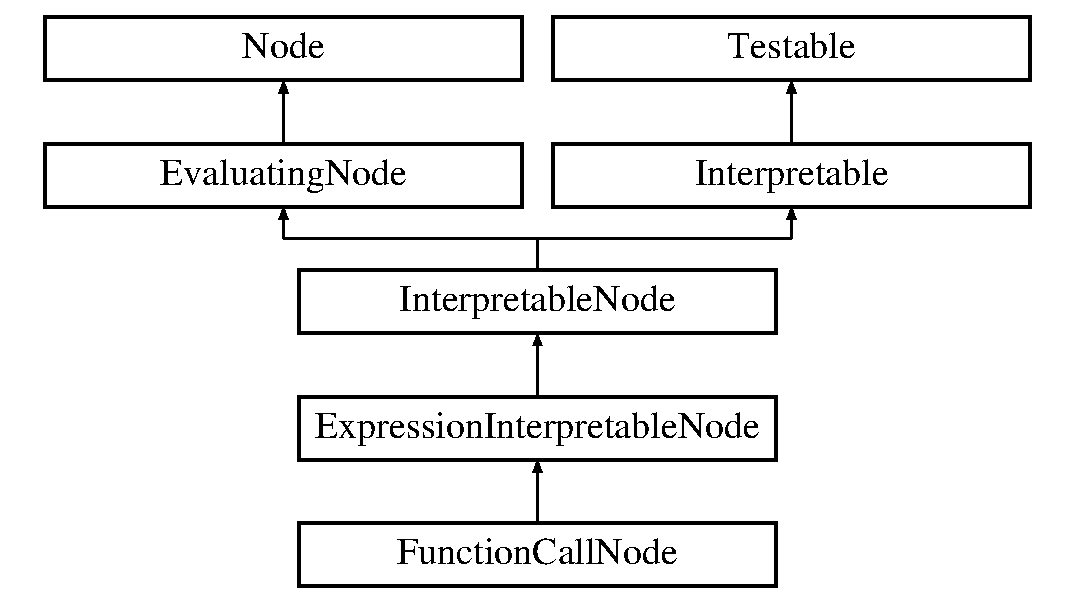
\includegraphics[height=5.000000cm]{classFunctionCallNode}
\end{center}
\end{figure}
\subsection*{Public Member Functions}
\begin{DoxyCompactItemize}
\item 
\hyperlink{classFunctionCallNode_af4c639d83ec4fc10ee4648277cedc134}{Function\+Call\+Node} ()
\item 
virtual \hyperlink{classFunctionCallNode_a781834ac40eada17d2f9dc53a8bd26e5}{$\sim$\+Function\+Call\+Node} ()
\item 
virtual void \hyperlink{classFunctionCallNode_a5a7f576984942e2e39057d716d8a5547}{test} (\hyperlink{classValidator}{Validator} $\ast$validator)
\item 
virtual \hyperlink{classValue}{Value} \hyperlink{classFunctionCallNode_a1d0d8806b7dd501ed43da58f77f7c49e}{interpret} (\hyperlink{classInterpreter}{Interpreter} $\ast$interpreter)
\item 
virtual void \hyperlink{classFunctionCallNode_a65f15b75804343caf5c4ce291460b1dc}{evaluate\+\_\+impl} (\hyperlink{classSystemHandler}{System\+Handler} $\ast$handler, \hyperlink{statics_8h_a6664c451ca7787483a7981cc1de68dbb}{E\+V\+A\+L\+U\+A\+T\+I\+O\+N\+\_\+\+T\+Y\+PE} expected\+\_\+evaluation, struct \hyperlink{structEvaluation}{Evaluation} $\ast$evaluation)
\end{DoxyCompactItemize}
\subsection*{Public Attributes}
\begin{DoxyCompactItemize}
\item 
\hyperlink{classIdentifierNode}{Identifier\+Node} $\ast$ \hyperlink{classFunctionCallNode_a03ebfc10277d6c6a7698b5eb0c02ac73}{name}
\item 
std\+::vector$<$ \hyperlink{classExpressionInterpretableNode}{Expression\+Interpretable\+Node} $\ast$ $>$ \hyperlink{classFunctionCallNode_a087579d1f0ece94640b4821830f72b55}{arguments}
\end{DoxyCompactItemize}
\subsection*{Additional Inherited Members}


\subsection{Constructor \& Destructor Documentation}
\mbox{\Hypertarget{classFunctionCallNode_af4c639d83ec4fc10ee4648277cedc134}\label{classFunctionCallNode_af4c639d83ec4fc10ee4648277cedc134}} 
\index{Function\+Call\+Node@{Function\+Call\+Node}!Function\+Call\+Node@{Function\+Call\+Node}}
\index{Function\+Call\+Node@{Function\+Call\+Node}!Function\+Call\+Node@{Function\+Call\+Node}}
\subsubsection{\texorpdfstring{Function\+Call\+Node()}{FunctionCallNode()}}
{\footnotesize\ttfamily Function\+Call\+Node\+::\+Function\+Call\+Node (\begin{DoxyParamCaption}{ }\end{DoxyParamCaption})}

\mbox{\Hypertarget{classFunctionCallNode_a781834ac40eada17d2f9dc53a8bd26e5}\label{classFunctionCallNode_a781834ac40eada17d2f9dc53a8bd26e5}} 
\index{Function\+Call\+Node@{Function\+Call\+Node}!````~Function\+Call\+Node@{$\sim$\+Function\+Call\+Node}}
\index{````~Function\+Call\+Node@{$\sim$\+Function\+Call\+Node}!Function\+Call\+Node@{Function\+Call\+Node}}
\subsubsection{\texorpdfstring{$\sim$\+Function\+Call\+Node()}{~FunctionCallNode()}}
{\footnotesize\ttfamily virtual Function\+Call\+Node\+::$\sim$\+Function\+Call\+Node (\begin{DoxyParamCaption}{ }\end{DoxyParamCaption})\hspace{0.3cm}{\ttfamily [virtual]}}



\subsection{Member Function Documentation}
\mbox{\Hypertarget{classFunctionCallNode_a65f15b75804343caf5c4ce291460b1dc}\label{classFunctionCallNode_a65f15b75804343caf5c4ce291460b1dc}} 
\index{Function\+Call\+Node@{Function\+Call\+Node}!evaluate\+\_\+impl@{evaluate\+\_\+impl}}
\index{evaluate\+\_\+impl@{evaluate\+\_\+impl}!Function\+Call\+Node@{Function\+Call\+Node}}
\subsubsection{\texorpdfstring{evaluate\+\_\+impl()}{evaluate\_impl()}}
{\footnotesize\ttfamily virtual void Function\+Call\+Node\+::evaluate\+\_\+impl (\begin{DoxyParamCaption}\item[{\hyperlink{classSystemHandler}{System\+Handler} $\ast$}]{handler,  }\item[{\hyperlink{statics_8h_a6664c451ca7787483a7981cc1de68dbb}{E\+V\+A\+L\+U\+A\+T\+I\+O\+N\+\_\+\+T\+Y\+PE}}]{expected\+\_\+evaluation,  }\item[{struct \hyperlink{structEvaluation}{Evaluation} $\ast$}]{evaluation }\end{DoxyParamCaption})\hspace{0.3cm}{\ttfamily [virtual]}}



Implements \hyperlink{classEvaluatingNode_a085fa06e0b46a93c814dc55cda0c1b26}{Evaluating\+Node}.

\mbox{\Hypertarget{classFunctionCallNode_a1d0d8806b7dd501ed43da58f77f7c49e}\label{classFunctionCallNode_a1d0d8806b7dd501ed43da58f77f7c49e}} 
\index{Function\+Call\+Node@{Function\+Call\+Node}!interpret@{interpret}}
\index{interpret@{interpret}!Function\+Call\+Node@{Function\+Call\+Node}}
\subsubsection{\texorpdfstring{interpret()}{interpret()}}
{\footnotesize\ttfamily virtual \hyperlink{classValue}{Value} Function\+Call\+Node\+::interpret (\begin{DoxyParamCaption}\item[{\hyperlink{classInterpreter}{Interpreter} $\ast$}]{interpreter }\end{DoxyParamCaption})\hspace{0.3cm}{\ttfamily [virtual]}}



Implements \hyperlink{classExpressionInterpretableNode_a43650f046c48fc539f77a207e3c9181e}{Expression\+Interpretable\+Node}.

\mbox{\Hypertarget{classFunctionCallNode_a5a7f576984942e2e39057d716d8a5547}\label{classFunctionCallNode_a5a7f576984942e2e39057d716d8a5547}} 
\index{Function\+Call\+Node@{Function\+Call\+Node}!test@{test}}
\index{test@{test}!Function\+Call\+Node@{Function\+Call\+Node}}
\subsubsection{\texorpdfstring{test()}{test()}}
{\footnotesize\ttfamily virtual void Function\+Call\+Node\+::test (\begin{DoxyParamCaption}\item[{\hyperlink{classValidator}{Validator} $\ast$}]{validator }\end{DoxyParamCaption})\hspace{0.3cm}{\ttfamily [virtual]}}



Reimplemented from \hyperlink{classInterpretable_a32f547aaf68dcbab993284d3257ab010}{Interpretable}.



\subsection{Member Data Documentation}
\mbox{\Hypertarget{classFunctionCallNode_a087579d1f0ece94640b4821830f72b55}\label{classFunctionCallNode_a087579d1f0ece94640b4821830f72b55}} 
\index{Function\+Call\+Node@{Function\+Call\+Node}!arguments@{arguments}}
\index{arguments@{arguments}!Function\+Call\+Node@{Function\+Call\+Node}}
\subsubsection{\texorpdfstring{arguments}{arguments}}
{\footnotesize\ttfamily std\+::vector$<$\hyperlink{classExpressionInterpretableNode}{Expression\+Interpretable\+Node}$\ast$$>$ Function\+Call\+Node\+::arguments}

\mbox{\Hypertarget{classFunctionCallNode_a03ebfc10277d6c6a7698b5eb0c02ac73}\label{classFunctionCallNode_a03ebfc10277d6c6a7698b5eb0c02ac73}} 
\index{Function\+Call\+Node@{Function\+Call\+Node}!name@{name}}
\index{name@{name}!Function\+Call\+Node@{Function\+Call\+Node}}
\subsubsection{\texorpdfstring{name}{name}}
{\footnotesize\ttfamily \hyperlink{classIdentifierNode}{Identifier\+Node}$\ast$ Function\+Call\+Node\+::name}



The documentation for this class was generated from the following file\+:\begin{DoxyCompactItemize}
\item 
include/\hyperlink{fcnode_8h}{fcnode.\+h}\end{DoxyCompactItemize}

\hypertarget{classFunctionNode}{}\section{Function\+Node Class Reference}
\label{classFunctionNode}\index{Function\+Node@{Function\+Node}}


{\ttfamily \#include $<$fnode.\+h$>$}

Inheritance diagram for Function\+Node\+:\begin{figure}[H]
\begin{center}
\leavevmode
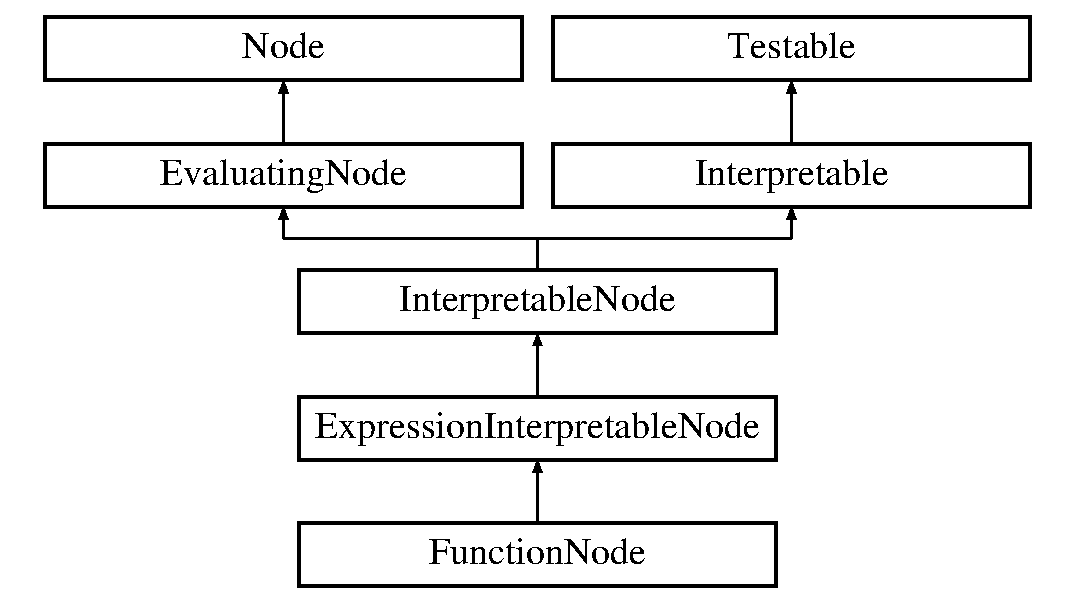
\includegraphics[height=5.000000cm]{classFunctionNode}
\end{center}
\end{figure}
\subsection*{Public Member Functions}
\begin{DoxyCompactItemize}
\item 
\hyperlink{classFunctionNode_ac4467a4c13382e0058cb2bd4fb70e0ab}{Function\+Node} ()
\item 
virtual \hyperlink{classFunctionNode_ad9c4a35db175de9386ac86d91a1a95df}{$\sim$\+Function\+Node} ()
\item 
virtual void \hyperlink{classFunctionNode_a1f020e7ea0181b3ce16ad2ef8426f773}{test} (\hyperlink{classValidator}{Validator} $\ast$validator)
\item 
virtual \hyperlink{classValue}{Value} \hyperlink{classFunctionNode_a059e6682cd51d0e126372a7af257ea5a}{interpret} (\hyperlink{classInterpreter}{Interpreter} $\ast$interpreter)
\item 
virtual void \hyperlink{classFunctionNode_a697f1fdc368f5ad09284b32b4466f353}{evaluate\+\_\+impl} (\hyperlink{classSystemHandler}{System\+Handler} $\ast$handler, \hyperlink{statics_8h_a6664c451ca7787483a7981cc1de68dbb}{E\+V\+A\+L\+U\+A\+T\+I\+O\+N\+\_\+\+T\+Y\+PE} expected\+\_\+evaluation, struct \hyperlink{structEvaluation}{Evaluation} $\ast$evaluation)
\end{DoxyCompactItemize}
\subsection*{Public Attributes}
\begin{DoxyCompactItemize}
\item 
std\+::string \hyperlink{classFunctionNode_a21284dd655c91da1f792dc3bc1bba60c}{name}
\item 
struct \hyperlink{classBodyNode}{Body\+Node} $\ast$ \hyperlink{classFunctionNode_a3ebe1489837aee643b7e9f626ef0976a}{body}
\item 
std\+::vector$<$ \hyperlink{classVarNode}{Var\+Node} $\ast$ $>$ \hyperlink{classFunctionNode_a04bfceaf29255ffd83195f669b5c37ef}{args}
\item 
\hyperlink{classNode}{Node} $\ast$ \hyperlink{classFunctionNode_a52768e57ce61d19f974c5c7412168377}{return\+\_\+type}
\end{DoxyCompactItemize}
\subsection*{Additional Inherited Members}


\subsection{Constructor \& Destructor Documentation}
\mbox{\Hypertarget{classFunctionNode_ac4467a4c13382e0058cb2bd4fb70e0ab}\label{classFunctionNode_ac4467a4c13382e0058cb2bd4fb70e0ab}} 
\index{Function\+Node@{Function\+Node}!Function\+Node@{Function\+Node}}
\index{Function\+Node@{Function\+Node}!Function\+Node@{Function\+Node}}
\subsubsection{\texorpdfstring{Function\+Node()}{FunctionNode()}}
{\footnotesize\ttfamily Function\+Node\+::\+Function\+Node (\begin{DoxyParamCaption}{ }\end{DoxyParamCaption})}

\mbox{\Hypertarget{classFunctionNode_ad9c4a35db175de9386ac86d91a1a95df}\label{classFunctionNode_ad9c4a35db175de9386ac86d91a1a95df}} 
\index{Function\+Node@{Function\+Node}!````~Function\+Node@{$\sim$\+Function\+Node}}
\index{````~Function\+Node@{$\sim$\+Function\+Node}!Function\+Node@{Function\+Node}}
\subsubsection{\texorpdfstring{$\sim$\+Function\+Node()}{~FunctionNode()}}
{\footnotesize\ttfamily virtual Function\+Node\+::$\sim$\+Function\+Node (\begin{DoxyParamCaption}{ }\end{DoxyParamCaption})\hspace{0.3cm}{\ttfamily [virtual]}}



\subsection{Member Function Documentation}
\mbox{\Hypertarget{classFunctionNode_a697f1fdc368f5ad09284b32b4466f353}\label{classFunctionNode_a697f1fdc368f5ad09284b32b4466f353}} 
\index{Function\+Node@{Function\+Node}!evaluate\+\_\+impl@{evaluate\+\_\+impl}}
\index{evaluate\+\_\+impl@{evaluate\+\_\+impl}!Function\+Node@{Function\+Node}}
\subsubsection{\texorpdfstring{evaluate\+\_\+impl()}{evaluate\_impl()}}
{\footnotesize\ttfamily virtual void Function\+Node\+::evaluate\+\_\+impl (\begin{DoxyParamCaption}\item[{\hyperlink{classSystemHandler}{System\+Handler} $\ast$}]{handler,  }\item[{\hyperlink{statics_8h_a6664c451ca7787483a7981cc1de68dbb}{E\+V\+A\+L\+U\+A\+T\+I\+O\+N\+\_\+\+T\+Y\+PE}}]{expected\+\_\+evaluation,  }\item[{struct \hyperlink{structEvaluation}{Evaluation} $\ast$}]{evaluation }\end{DoxyParamCaption})\hspace{0.3cm}{\ttfamily [virtual]}}



Implements \hyperlink{classEvaluatingNode_a085fa06e0b46a93c814dc55cda0c1b26}{Evaluating\+Node}.

\mbox{\Hypertarget{classFunctionNode_a059e6682cd51d0e126372a7af257ea5a}\label{classFunctionNode_a059e6682cd51d0e126372a7af257ea5a}} 
\index{Function\+Node@{Function\+Node}!interpret@{interpret}}
\index{interpret@{interpret}!Function\+Node@{Function\+Node}}
\subsubsection{\texorpdfstring{interpret()}{interpret()}}
{\footnotesize\ttfamily virtual \hyperlink{classValue}{Value} Function\+Node\+::interpret (\begin{DoxyParamCaption}\item[{\hyperlink{classInterpreter}{Interpreter} $\ast$}]{interpreter }\end{DoxyParamCaption})\hspace{0.3cm}{\ttfamily [virtual]}}



Implements \hyperlink{classExpressionInterpretableNode_a43650f046c48fc539f77a207e3c9181e}{Expression\+Interpretable\+Node}.

\mbox{\Hypertarget{classFunctionNode_a1f020e7ea0181b3ce16ad2ef8426f773}\label{classFunctionNode_a1f020e7ea0181b3ce16ad2ef8426f773}} 
\index{Function\+Node@{Function\+Node}!test@{test}}
\index{test@{test}!Function\+Node@{Function\+Node}}
\subsubsection{\texorpdfstring{test()}{test()}}
{\footnotesize\ttfamily virtual void Function\+Node\+::test (\begin{DoxyParamCaption}\item[{\hyperlink{classValidator}{Validator} $\ast$}]{validator }\end{DoxyParamCaption})\hspace{0.3cm}{\ttfamily [virtual]}}



Reimplemented from \hyperlink{classInterpretable_a32f547aaf68dcbab993284d3257ab010}{Interpretable}.



\subsection{Member Data Documentation}
\mbox{\Hypertarget{classFunctionNode_a04bfceaf29255ffd83195f669b5c37ef}\label{classFunctionNode_a04bfceaf29255ffd83195f669b5c37ef}} 
\index{Function\+Node@{Function\+Node}!args@{args}}
\index{args@{args}!Function\+Node@{Function\+Node}}
\subsubsection{\texorpdfstring{args}{args}}
{\footnotesize\ttfamily std\+::vector$<$\hyperlink{classVarNode}{Var\+Node}$\ast$$>$ Function\+Node\+::args}

\mbox{\Hypertarget{classFunctionNode_a3ebe1489837aee643b7e9f626ef0976a}\label{classFunctionNode_a3ebe1489837aee643b7e9f626ef0976a}} 
\index{Function\+Node@{Function\+Node}!body@{body}}
\index{body@{body}!Function\+Node@{Function\+Node}}
\subsubsection{\texorpdfstring{body}{body}}
{\footnotesize\ttfamily struct \hyperlink{classBodyNode}{Body\+Node}$\ast$ Function\+Node\+::body}

\mbox{\Hypertarget{classFunctionNode_a21284dd655c91da1f792dc3bc1bba60c}\label{classFunctionNode_a21284dd655c91da1f792dc3bc1bba60c}} 
\index{Function\+Node@{Function\+Node}!name@{name}}
\index{name@{name}!Function\+Node@{Function\+Node}}
\subsubsection{\texorpdfstring{name}{name}}
{\footnotesize\ttfamily std\+::string Function\+Node\+::name}

\mbox{\Hypertarget{classFunctionNode_a52768e57ce61d19f974c5c7412168377}\label{classFunctionNode_a52768e57ce61d19f974c5c7412168377}} 
\index{Function\+Node@{Function\+Node}!return\+\_\+type@{return\+\_\+type}}
\index{return\+\_\+type@{return\+\_\+type}!Function\+Node@{Function\+Node}}
\subsubsection{\texorpdfstring{return\+\_\+type}{return\_type}}
{\footnotesize\ttfamily \hyperlink{classNode}{Node}$\ast$ Function\+Node\+::return\+\_\+type}



The documentation for this class was generated from the following file\+:\begin{DoxyCompactItemize}
\item 
include/\hyperlink{fnode_8h}{fnode.\+h}\end{DoxyCompactItemize}

\hypertarget{classFunctionSystem}{}\section{Function\+System Class Reference}
\label{classFunctionSystem}\index{Function\+System@{Function\+System}}


{\ttfamily \#include $<$functionsystem.\+h$>$}

Inheritance diagram for Function\+System\+:\begin{figure}[H]
\begin{center}
\leavevmode
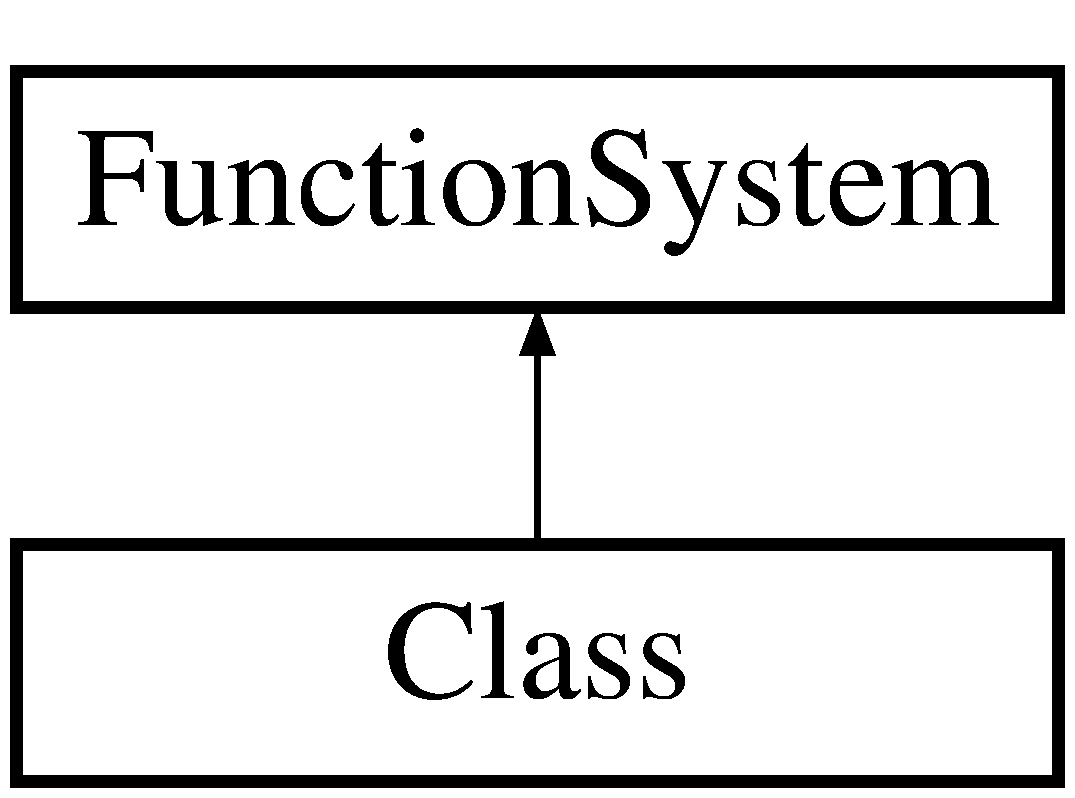
\includegraphics[height=2.000000cm]{classFunctionSystem}
\end{center}
\end{figure}
\subsection*{Public Member Functions}
\begin{DoxyCompactItemize}
\item 
\hyperlink{classFunctionSystem_a66e3b5e5118f00a940c3e4a2f138c9c6}{Function\+System} ()
\item 
\hyperlink{classFunctionSystem_acad46fc5783fee1962d2450ea181f310}{Function\+System} (\hyperlink{classInterpreter}{Interpreter} $\ast$interpreter)
\item 
\hyperlink{classFunctionSystem_a720ae7e377cda0548bd8f1ef3c9390d9}{Function\+System} (\hyperlink{classInterpreter}{Interpreter} $\ast$interpreter, \hyperlink{classFunctionSystem}{Function\+System} $\ast$\hyperlink{classFunctionSystem_a0d223ca42b6d6617af61136bdb1f33dd}{prev\+\_\+fc\+\_\+sys})
\item 
virtual \hyperlink{classFunctionSystem_ad6f794406996091d08df65e8d3e0e665}{$\sim$\+Function\+System} ()
\item 
void \hyperlink{classFunctionSystem_a70175d76b5b377e58b1d3b0eebd1bc0a}{set\+Interpreter} (\hyperlink{classInterpreter}{Interpreter} $\ast$interpreter)
\item 
\hyperlink{classFunction}{Function} $\ast$ \hyperlink{classFunctionSystem_a975b09fef826151dd66dece595aa452b}{register\+Function} (std\+::string name, std\+::function$<$ void(std\+::vector$<$ \hyperlink{classValue}{Value} $>$ values, \hyperlink{classValue}{Value} $\ast$return\+\_\+value, std\+::shared\+\_\+ptr$<$ \hyperlink{classObject}{Object} $>$ object)$>$ entrypoint)
\item 
\hyperlink{classFunction}{Function} $\ast$ \hyperlink{classFunctionSystem_a1a3d54c912c91ea7656cc5a6185a9a6f}{register\+Function} (\hyperlink{classFunctionNode}{Function\+Node} $\ast$fnode)
\item 
bool \hyperlink{classFunctionSystem_a7248f494dea505ffaa2108b202f1efcb}{has\+Function} (std\+::string name)
\item 
bool \hyperlink{classFunctionSystem_a5bb3f64848489ff7cc4c982c08a10eaa}{has\+Function\+Locally} (std\+::string name)
\item 
\hyperlink{classFunction}{Function} $\ast$ \hyperlink{classFunctionSystem_a6ccd76d0760272b64790d6f5c8cdc607}{get\+Function\+By\+Name} (std\+::string name)
\end{DoxyCompactItemize}
\subsection*{Public Attributes}
\begin{DoxyCompactItemize}
\item 
\hyperlink{classFunctionSystem}{Function\+System} $\ast$ \hyperlink{classFunctionSystem_a0d223ca42b6d6617af61136bdb1f33dd}{prev\+\_\+fc\+\_\+sys}
\item 
std\+::shared\+\_\+ptr$<$ \hyperlink{classObject}{Object} $>$ \hyperlink{classFunctionSystem_a59f2a49d91338ced0a79d3898412fcaf}{current\+Obj}
\end{DoxyCompactItemize}


\subsection{Constructor \& Destructor Documentation}
\mbox{\Hypertarget{classFunctionSystem_a66e3b5e5118f00a940c3e4a2f138c9c6}\label{classFunctionSystem_a66e3b5e5118f00a940c3e4a2f138c9c6}} 
\index{Function\+System@{Function\+System}!Function\+System@{Function\+System}}
\index{Function\+System@{Function\+System}!Function\+System@{Function\+System}}
\subsubsection{\texorpdfstring{Function\+System()}{FunctionSystem()}\hspace{0.1cm}{\footnotesize\ttfamily [1/3]}}
{\footnotesize\ttfamily Function\+System\+::\+Function\+System (\begin{DoxyParamCaption}{ }\end{DoxyParamCaption})}

\mbox{\Hypertarget{classFunctionSystem_acad46fc5783fee1962d2450ea181f310}\label{classFunctionSystem_acad46fc5783fee1962d2450ea181f310}} 
\index{Function\+System@{Function\+System}!Function\+System@{Function\+System}}
\index{Function\+System@{Function\+System}!Function\+System@{Function\+System}}
\subsubsection{\texorpdfstring{Function\+System()}{FunctionSystem()}\hspace{0.1cm}{\footnotesize\ttfamily [2/3]}}
{\footnotesize\ttfamily Function\+System\+::\+Function\+System (\begin{DoxyParamCaption}\item[{\hyperlink{classInterpreter}{Interpreter} $\ast$}]{interpreter }\end{DoxyParamCaption})}

\mbox{\Hypertarget{classFunctionSystem_a720ae7e377cda0548bd8f1ef3c9390d9}\label{classFunctionSystem_a720ae7e377cda0548bd8f1ef3c9390d9}} 
\index{Function\+System@{Function\+System}!Function\+System@{Function\+System}}
\index{Function\+System@{Function\+System}!Function\+System@{Function\+System}}
\subsubsection{\texorpdfstring{Function\+System()}{FunctionSystem()}\hspace{0.1cm}{\footnotesize\ttfamily [3/3]}}
{\footnotesize\ttfamily Function\+System\+::\+Function\+System (\begin{DoxyParamCaption}\item[{\hyperlink{classInterpreter}{Interpreter} $\ast$}]{interpreter,  }\item[{\hyperlink{classFunctionSystem}{Function\+System} $\ast$}]{prev\+\_\+fc\+\_\+sys }\end{DoxyParamCaption})}

\mbox{\Hypertarget{classFunctionSystem_ad6f794406996091d08df65e8d3e0e665}\label{classFunctionSystem_ad6f794406996091d08df65e8d3e0e665}} 
\index{Function\+System@{Function\+System}!````~Function\+System@{$\sim$\+Function\+System}}
\index{````~Function\+System@{$\sim$\+Function\+System}!Function\+System@{Function\+System}}
\subsubsection{\texorpdfstring{$\sim$\+Function\+System()}{~FunctionSystem()}}
{\footnotesize\ttfamily virtual Function\+System\+::$\sim$\+Function\+System (\begin{DoxyParamCaption}{ }\end{DoxyParamCaption})\hspace{0.3cm}{\ttfamily [virtual]}}



\subsection{Member Function Documentation}
\mbox{\Hypertarget{classFunctionSystem_a6ccd76d0760272b64790d6f5c8cdc607}\label{classFunctionSystem_a6ccd76d0760272b64790d6f5c8cdc607}} 
\index{Function\+System@{Function\+System}!get\+Function\+By\+Name@{get\+Function\+By\+Name}}
\index{get\+Function\+By\+Name@{get\+Function\+By\+Name}!Function\+System@{Function\+System}}
\subsubsection{\texorpdfstring{get\+Function\+By\+Name()}{getFunctionByName()}}
{\footnotesize\ttfamily \hyperlink{classFunction}{Function}$\ast$ Function\+System\+::get\+Function\+By\+Name (\begin{DoxyParamCaption}\item[{std\+::string}]{name }\end{DoxyParamCaption})}

\mbox{\Hypertarget{classFunctionSystem_a7248f494dea505ffaa2108b202f1efcb}\label{classFunctionSystem_a7248f494dea505ffaa2108b202f1efcb}} 
\index{Function\+System@{Function\+System}!has\+Function@{has\+Function}}
\index{has\+Function@{has\+Function}!Function\+System@{Function\+System}}
\subsubsection{\texorpdfstring{has\+Function()}{hasFunction()}}
{\footnotesize\ttfamily bool Function\+System\+::has\+Function (\begin{DoxyParamCaption}\item[{std\+::string}]{name }\end{DoxyParamCaption})}

\mbox{\Hypertarget{classFunctionSystem_a5bb3f64848489ff7cc4c982c08a10eaa}\label{classFunctionSystem_a5bb3f64848489ff7cc4c982c08a10eaa}} 
\index{Function\+System@{Function\+System}!has\+Function\+Locally@{has\+Function\+Locally}}
\index{has\+Function\+Locally@{has\+Function\+Locally}!Function\+System@{Function\+System}}
\subsubsection{\texorpdfstring{has\+Function\+Locally()}{hasFunctionLocally()}}
{\footnotesize\ttfamily bool Function\+System\+::has\+Function\+Locally (\begin{DoxyParamCaption}\item[{std\+::string}]{name }\end{DoxyParamCaption})}

\mbox{\Hypertarget{classFunctionSystem_a975b09fef826151dd66dece595aa452b}\label{classFunctionSystem_a975b09fef826151dd66dece595aa452b}} 
\index{Function\+System@{Function\+System}!register\+Function@{register\+Function}}
\index{register\+Function@{register\+Function}!Function\+System@{Function\+System}}
\subsubsection{\texorpdfstring{register\+Function()}{registerFunction()}\hspace{0.1cm}{\footnotesize\ttfamily [1/2]}}
{\footnotesize\ttfamily \hyperlink{classFunction}{Function}$\ast$ Function\+System\+::register\+Function (\begin{DoxyParamCaption}\item[{std\+::string}]{name,  }\item[{std\+::function$<$ void(std\+::vector$<$ \hyperlink{classValue}{Value} $>$ values, \hyperlink{classValue}{Value} $\ast$return\+\_\+value, std\+::shared\+\_\+ptr$<$ \hyperlink{classObject}{Object} $>$ object)$>$}]{entrypoint }\end{DoxyParamCaption})}

Creates and registers a \hyperlink{classNativeFunction}{Native\+Function} into the \hyperlink{classFunctionSystem}{Function\+System} and when the function is called the {\bfseries entrypoint} lambda function provided will be invoked. 
\begin{DoxyParams}{Parameters}
{\em name} & The name of the function to create \\
\hline
{\em entrypoint} & The entrypoint of the function. \\
\hline
\end{DoxyParams}
\mbox{\Hypertarget{classFunctionSystem_a1a3d54c912c91ea7656cc5a6185a9a6f}\label{classFunctionSystem_a1a3d54c912c91ea7656cc5a6185a9a6f}} 
\index{Function\+System@{Function\+System}!register\+Function@{register\+Function}}
\index{register\+Function@{register\+Function}!Function\+System@{Function\+System}}
\subsubsection{\texorpdfstring{register\+Function()}{registerFunction()}\hspace{0.1cm}{\footnotesize\ttfamily [2/2]}}
{\footnotesize\ttfamily \hyperlink{classFunction}{Function}$\ast$ Function\+System\+::register\+Function (\begin{DoxyParamCaption}\item[{\hyperlink{classFunctionNode}{Function\+Node} $\ast$}]{fnode }\end{DoxyParamCaption})}

\mbox{\Hypertarget{classFunctionSystem_a70175d76b5b377e58b1d3b0eebd1bc0a}\label{classFunctionSystem_a70175d76b5b377e58b1d3b0eebd1bc0a}} 
\index{Function\+System@{Function\+System}!set\+Interpreter@{set\+Interpreter}}
\index{set\+Interpreter@{set\+Interpreter}!Function\+System@{Function\+System}}
\subsubsection{\texorpdfstring{set\+Interpreter()}{setInterpreter()}}
{\footnotesize\ttfamily void Function\+System\+::set\+Interpreter (\begin{DoxyParamCaption}\item[{\hyperlink{classInterpreter}{Interpreter} $\ast$}]{interpreter }\end{DoxyParamCaption})}



\subsection{Member Data Documentation}
\mbox{\Hypertarget{classFunctionSystem_a59f2a49d91338ced0a79d3898412fcaf}\label{classFunctionSystem_a59f2a49d91338ced0a79d3898412fcaf}} 
\index{Function\+System@{Function\+System}!current\+Obj@{current\+Obj}}
\index{current\+Obj@{current\+Obj}!Function\+System@{Function\+System}}
\subsubsection{\texorpdfstring{current\+Obj}{currentObj}}
{\footnotesize\ttfamily std\+::shared\+\_\+ptr$<$\hyperlink{classObject}{Object}$>$ Function\+System\+::current\+Obj}

Set to an \hyperlink{classObject}{Object} instance when calling an \hyperlink{classObject}{Object} \hyperlink{classClass}{Class} \hyperlink{classFunction}{Function} through an object access expression such as {\itshape Foo.\+Bar();} \begin{DoxyNote}{Note}
This is useful for when the right node of an expression needs to know the current object of the left node 
\end{DoxyNote}
\begin{DoxyAttention}{Attention}
this should only be used during an object access expression 
\end{DoxyAttention}
\mbox{\Hypertarget{classFunctionSystem_a0d223ca42b6d6617af61136bdb1f33dd}\label{classFunctionSystem_a0d223ca42b6d6617af61136bdb1f33dd}} 
\index{Function\+System@{Function\+System}!prev\+\_\+fc\+\_\+sys@{prev\+\_\+fc\+\_\+sys}}
\index{prev\+\_\+fc\+\_\+sys@{prev\+\_\+fc\+\_\+sys}!Function\+System@{Function\+System}}
\subsubsection{\texorpdfstring{prev\+\_\+fc\+\_\+sys}{prev\_fc\_sys}}
{\footnotesize\ttfamily \hyperlink{classFunctionSystem}{Function\+System}$\ast$ Function\+System\+::prev\+\_\+fc\+\_\+sys}

The previous, parent function system. Set to N\+U\+LL if no parent exists. \begin{DoxyNote}{Note}
This is used for classes that extend other classes 
\end{DoxyNote}
\begin{DoxySeeAlso}{See also}
\hyperlink{classFunctionSystem_a6ccd76d0760272b64790d6f5c8cdc607}{get\+Function\+By\+Name} 
\end{DoxySeeAlso}


The documentation for this class was generated from the following file\+:\begin{DoxyCompactItemize}
\item 
include/\hyperlink{functionsystem_8h}{functionsystem.\+h}\end{DoxyCompactItemize}

\hypertarget{classGroupedFunction}{}\section{Grouped\+Function Class Reference}
\label{classGroupedFunction}\index{Grouped\+Function@{Grouped\+Function}}


{\ttfamily \#include $<$groupedfunction.\+h$>$}

Inheritance diagram for Grouped\+Function\+:\begin{figure}[H]
\begin{center}
\leavevmode
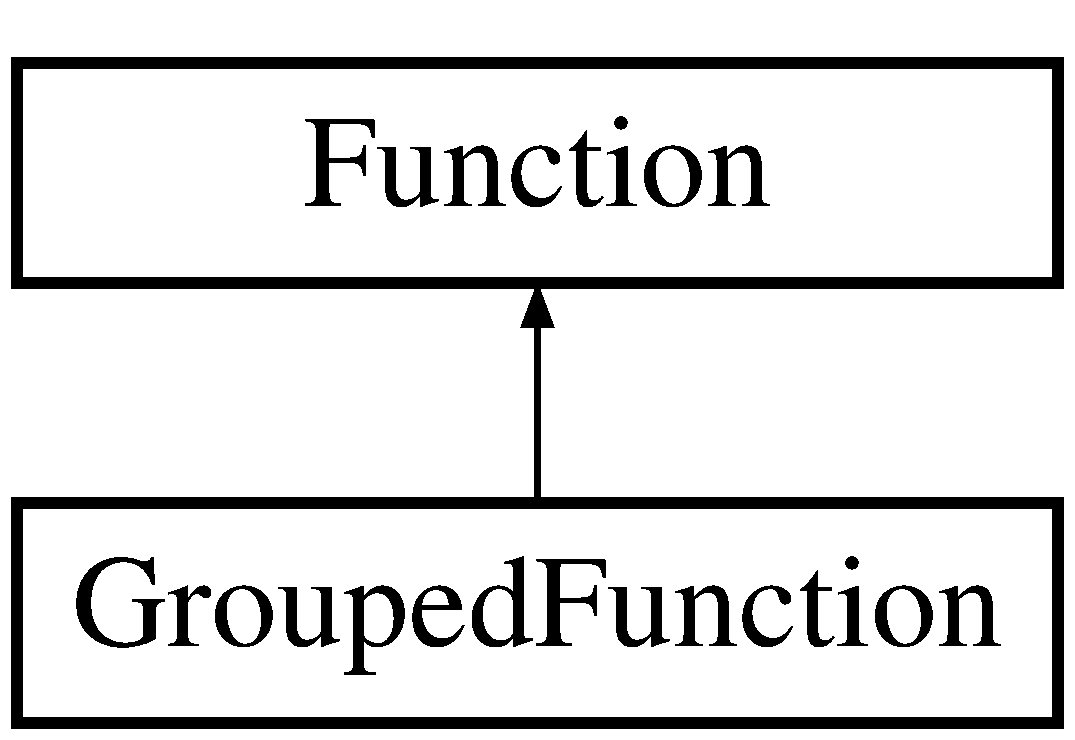
\includegraphics[height=2.000000cm]{classGroupedFunction}
\end{center}
\end{figure}
\subsection*{Public Member Functions}
\begin{DoxyCompactItemize}
\item 
\hyperlink{classGroupedFunction_a613f536552aeb5b85e363d8f5b24a87f}{Grouped\+Function} (std\+::string \hyperlink{classFunction_a161d1ceb4f67f3222caf429fea7b71f1}{name}, \hyperlink{classSystemHandler}{System\+Handler} $\ast$\hyperlink{classGroupedFunction_a932d46ac0e35f1a1c989427e51c1b2b4}{sys\+\_\+handler})
\item 
virtual \hyperlink{classGroupedFunction_a5f3c1ed74083a0b9f1dea5ae2f287e70}{$\sim$\+Grouped\+Function} ()
\item 
virtual void \hyperlink{classGroupedFunction_a90a74bd39250863046a7cb97ce013d2b}{invoke} (std\+::vector$<$ \hyperlink{classValue}{Value} $>$ values, \hyperlink{classValue}{Value} $\ast$return\+\_\+value, std\+::shared\+\_\+ptr$<$ \hyperlink{classObject}{Object} $>$ object)
\item 
\hyperlink{classFunction}{Function} $\ast$ \hyperlink{classGroupedFunction_a216ffc5f08fe1bc61968f4a5f5e99b49}{get\+Function\+For\+Values} (std\+::vector$<$ \hyperlink{classValue}{Value} $>$ values)
\item 
\hyperlink{classFunction}{Function} $\ast$ \hyperlink{classGroupedFunction_a4aa6efd8e1ec521964b7826249458f27}{get\+Function\+For\+Arguments} (std\+::vector$<$ \hyperlink{classVarType}{Var\+Type} $>$ types)
\item 
bool \hyperlink{classGroupedFunction_a40cb1ca76aaf883d8c8af39b33eaa74b}{has\+Function\+With\+Arguments} (std\+::vector$<$ \hyperlink{classVarType}{Var\+Type} $>$ types)
\item 
void \hyperlink{classGroupedFunction_ab019d13e239da992fc6fbe01bc5be8ef}{add\+Function} (std\+::unique\+\_\+ptr$<$ \hyperlink{classFunction}{Function} $>$ function)
\end{DoxyCompactItemize}
\subsection*{Public Attributes}
\begin{DoxyCompactItemize}
\item 
\hyperlink{classSystemHandler}{System\+Handler} $\ast$ \hyperlink{classGroupedFunction_a932d46ac0e35f1a1c989427e51c1b2b4}{sys\+\_\+handler}
\end{DoxyCompactItemize}


\subsection{Constructor \& Destructor Documentation}
\mbox{\Hypertarget{classGroupedFunction_a613f536552aeb5b85e363d8f5b24a87f}\label{classGroupedFunction_a613f536552aeb5b85e363d8f5b24a87f}} 
\index{Grouped\+Function@{Grouped\+Function}!Grouped\+Function@{Grouped\+Function}}
\index{Grouped\+Function@{Grouped\+Function}!Grouped\+Function@{Grouped\+Function}}
\subsubsection{\texorpdfstring{Grouped\+Function()}{GroupedFunction()}}
{\footnotesize\ttfamily Grouped\+Function\+::\+Grouped\+Function (\begin{DoxyParamCaption}\item[{std\+::string}]{name,  }\item[{\hyperlink{classSystemHandler}{System\+Handler} $\ast$}]{sys\+\_\+handler }\end{DoxyParamCaption})}

\mbox{\Hypertarget{classGroupedFunction_a5f3c1ed74083a0b9f1dea5ae2f287e70}\label{classGroupedFunction_a5f3c1ed74083a0b9f1dea5ae2f287e70}} 
\index{Grouped\+Function@{Grouped\+Function}!````~Grouped\+Function@{$\sim$\+Grouped\+Function}}
\index{````~Grouped\+Function@{$\sim$\+Grouped\+Function}!Grouped\+Function@{Grouped\+Function}}
\subsubsection{\texorpdfstring{$\sim$\+Grouped\+Function()}{~GroupedFunction()}}
{\footnotesize\ttfamily virtual Grouped\+Function\+::$\sim$\+Grouped\+Function (\begin{DoxyParamCaption}{ }\end{DoxyParamCaption})\hspace{0.3cm}{\ttfamily [virtual]}}



\subsection{Member Function Documentation}
\mbox{\Hypertarget{classGroupedFunction_ab019d13e239da992fc6fbe01bc5be8ef}\label{classGroupedFunction_ab019d13e239da992fc6fbe01bc5be8ef}} 
\index{Grouped\+Function@{Grouped\+Function}!add\+Function@{add\+Function}}
\index{add\+Function@{add\+Function}!Grouped\+Function@{Grouped\+Function}}
\subsubsection{\texorpdfstring{add\+Function()}{addFunction()}}
{\footnotesize\ttfamily void Grouped\+Function\+::add\+Function (\begin{DoxyParamCaption}\item[{std\+::unique\+\_\+ptr$<$ \hyperlink{classFunction}{Function} $>$}]{function }\end{DoxyParamCaption})}

\mbox{\Hypertarget{classGroupedFunction_a4aa6efd8e1ec521964b7826249458f27}\label{classGroupedFunction_a4aa6efd8e1ec521964b7826249458f27}} 
\index{Grouped\+Function@{Grouped\+Function}!get\+Function\+For\+Arguments@{get\+Function\+For\+Arguments}}
\index{get\+Function\+For\+Arguments@{get\+Function\+For\+Arguments}!Grouped\+Function@{Grouped\+Function}}
\subsubsection{\texorpdfstring{get\+Function\+For\+Arguments()}{getFunctionForArguments()}}
{\footnotesize\ttfamily \hyperlink{classFunction}{Function}$\ast$ Grouped\+Function\+::get\+Function\+For\+Arguments (\begin{DoxyParamCaption}\item[{std\+::vector$<$ \hyperlink{classVarType}{Var\+Type} $>$}]{types }\end{DoxyParamCaption})}

\mbox{\Hypertarget{classGroupedFunction_a216ffc5f08fe1bc61968f4a5f5e99b49}\label{classGroupedFunction_a216ffc5f08fe1bc61968f4a5f5e99b49}} 
\index{Grouped\+Function@{Grouped\+Function}!get\+Function\+For\+Values@{get\+Function\+For\+Values}}
\index{get\+Function\+For\+Values@{get\+Function\+For\+Values}!Grouped\+Function@{Grouped\+Function}}
\subsubsection{\texorpdfstring{get\+Function\+For\+Values()}{getFunctionForValues()}}
{\footnotesize\ttfamily \hyperlink{classFunction}{Function}$\ast$ Grouped\+Function\+::get\+Function\+For\+Values (\begin{DoxyParamCaption}\item[{std\+::vector$<$ \hyperlink{classValue}{Value} $>$}]{values }\end{DoxyParamCaption})}

\mbox{\Hypertarget{classGroupedFunction_a40cb1ca76aaf883d8c8af39b33eaa74b}\label{classGroupedFunction_a40cb1ca76aaf883d8c8af39b33eaa74b}} 
\index{Grouped\+Function@{Grouped\+Function}!has\+Function\+With\+Arguments@{has\+Function\+With\+Arguments}}
\index{has\+Function\+With\+Arguments@{has\+Function\+With\+Arguments}!Grouped\+Function@{Grouped\+Function}}
\subsubsection{\texorpdfstring{has\+Function\+With\+Arguments()}{hasFunctionWithArguments()}}
{\footnotesize\ttfamily bool Grouped\+Function\+::has\+Function\+With\+Arguments (\begin{DoxyParamCaption}\item[{std\+::vector$<$ \hyperlink{classVarType}{Var\+Type} $>$}]{types }\end{DoxyParamCaption})}

\mbox{\Hypertarget{classGroupedFunction_a90a74bd39250863046a7cb97ce013d2b}\label{classGroupedFunction_a90a74bd39250863046a7cb97ce013d2b}} 
\index{Grouped\+Function@{Grouped\+Function}!invoke@{invoke}}
\index{invoke@{invoke}!Grouped\+Function@{Grouped\+Function}}
\subsubsection{\texorpdfstring{invoke()}{invoke()}}
{\footnotesize\ttfamily virtual void Grouped\+Function\+::invoke (\begin{DoxyParamCaption}\item[{std\+::vector$<$ \hyperlink{classValue}{Value} $>$}]{values,  }\item[{\hyperlink{classValue}{Value} $\ast$}]{return\+\_\+value,  }\item[{std\+::shared\+\_\+ptr$<$ \hyperlink{classObject}{Object} $>$}]{object }\end{DoxyParamCaption})\hspace{0.3cm}{\ttfamily [virtual]}}

Invokes the correct function in this grouped function based on the values provided. If no function is found with the appropriate arguments for the input values then an exception is thrown.


\begin{DoxyParams}{Parameters}
{\em values} & The values to pass to the function to be called \\
\hline
{\em return\+\_\+value} & The return value for this function. \\
\hline
{\em object} & The object this function was invoked on. Set to N\+U\+LL if no object was provided. \\
\hline
\end{DoxyParams}

\begin{DoxyExceptions}{Exceptions}
{\em std\+::logic\+\_\+error} & Thrown if no function can be found that can deal with the values provided. \\
\hline
\end{DoxyExceptions}


Implements \hyperlink{classFunction_a84f9a63e68becc27e58ea738ba4cd698}{Function}.



\subsection{Member Data Documentation}
\mbox{\Hypertarget{classGroupedFunction_a932d46ac0e35f1a1c989427e51c1b2b4}\label{classGroupedFunction_a932d46ac0e35f1a1c989427e51c1b2b4}} 
\index{Grouped\+Function@{Grouped\+Function}!sys\+\_\+handler@{sys\+\_\+handler}}
\index{sys\+\_\+handler@{sys\+\_\+handler}!Grouped\+Function@{Grouped\+Function}}
\subsubsection{\texorpdfstring{sys\+\_\+handler}{sys\_handler}}
{\footnotesize\ttfamily \hyperlink{classSystemHandler}{System\+Handler}$\ast$ Grouped\+Function\+::sys\+\_\+handler}



The documentation for this class was generated from the following file\+:\begin{DoxyCompactItemize}
\item 
include/\hyperlink{groupedfunction_8h}{groupedfunction.\+h}\end{DoxyCompactItemize}

\hypertarget{classIdentifierNode}{}\section{Identifier\+Node Class Reference}
\label{classIdentifierNode}\index{Identifier\+Node@{Identifier\+Node}}


{\ttfamily \#include $<$identifiernode.\+h$>$}

Inheritance diagram for Identifier\+Node\+:\begin{figure}[H]
\begin{center}
\leavevmode
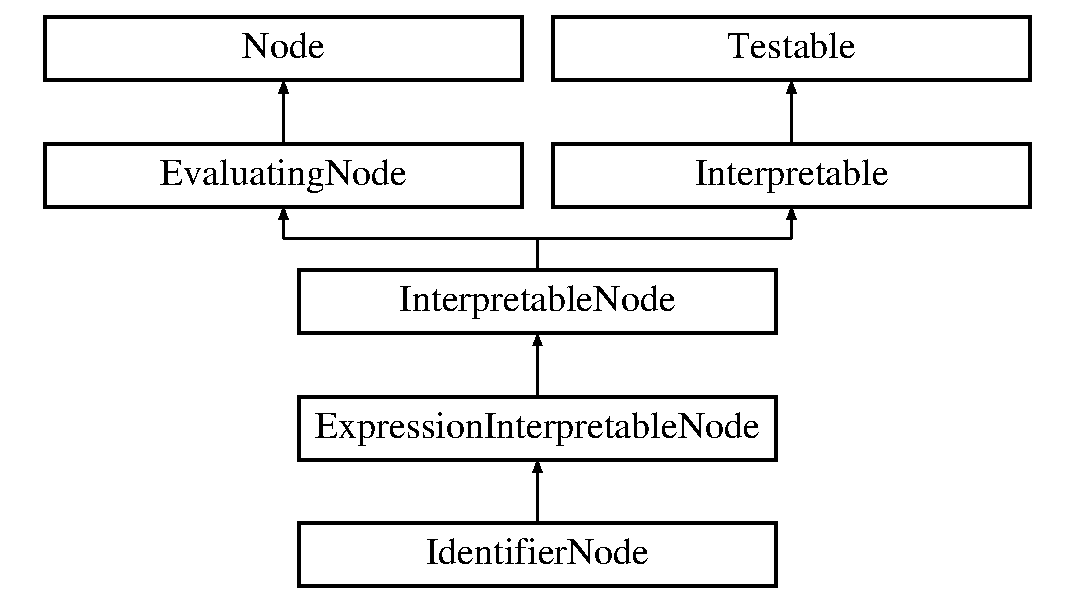
\includegraphics[height=5.000000cm]{classIdentifierNode}
\end{center}
\end{figure}
\subsection*{Public Member Functions}
\begin{DoxyCompactItemize}
\item 
\hyperlink{classIdentifierNode_ad12eaa3766a9650ce45b8188a9943755}{Identifier\+Node} ()
\item 
virtual \hyperlink{classIdentifierNode_a1c6fac2ceb5c9b7a435006b41898aa31}{$\sim$\+Identifier\+Node} ()
\item 
virtual void \hyperlink{classIdentifierNode_a1459965d8f22ade30cb78b2a1d60dd07}{test} (\hyperlink{classValidator}{Validator} $\ast$validator)
\item 
virtual \hyperlink{classValue}{Value} \hyperlink{classIdentifierNode_aa7be7da3e018352f8b549fcac3a8155a}{interpret} (\hyperlink{classInterpreter}{Interpreter} $\ast$interpreter)
\item 
virtual void \hyperlink{classIdentifierNode_a4960a1e68623066e413f8c2d68cee7e5}{evaluate\+\_\+impl} (\hyperlink{classSystemHandler}{System\+Handler} $\ast$handler, \hyperlink{statics_8h_a6664c451ca7787483a7981cc1de68dbb}{E\+V\+A\+L\+U\+A\+T\+I\+O\+N\+\_\+\+T\+Y\+PE} expected\+\_\+evaluation, struct \hyperlink{structEvaluation}{Evaluation} $\ast$evaluation)
\end{DoxyCompactItemize}
\subsection*{Public Attributes}
\begin{DoxyCompactItemize}
\item 
std\+::string \hyperlink{classIdentifierNode_a7d92bad6e678bdff5f87f53bd55a53fb}{value}
\end{DoxyCompactItemize}
\subsection*{Additional Inherited Members}


\subsection{Constructor \& Destructor Documentation}
\mbox{\Hypertarget{classIdentifierNode_ad12eaa3766a9650ce45b8188a9943755}\label{classIdentifierNode_ad12eaa3766a9650ce45b8188a9943755}} 
\index{Identifier\+Node@{Identifier\+Node}!Identifier\+Node@{Identifier\+Node}}
\index{Identifier\+Node@{Identifier\+Node}!Identifier\+Node@{Identifier\+Node}}
\subsubsection{\texorpdfstring{Identifier\+Node()}{IdentifierNode()}}
{\footnotesize\ttfamily Identifier\+Node\+::\+Identifier\+Node (\begin{DoxyParamCaption}{ }\end{DoxyParamCaption})}

\mbox{\Hypertarget{classIdentifierNode_a1c6fac2ceb5c9b7a435006b41898aa31}\label{classIdentifierNode_a1c6fac2ceb5c9b7a435006b41898aa31}} 
\index{Identifier\+Node@{Identifier\+Node}!````~Identifier\+Node@{$\sim$\+Identifier\+Node}}
\index{````~Identifier\+Node@{$\sim$\+Identifier\+Node}!Identifier\+Node@{Identifier\+Node}}
\subsubsection{\texorpdfstring{$\sim$\+Identifier\+Node()}{~IdentifierNode()}}
{\footnotesize\ttfamily virtual Identifier\+Node\+::$\sim$\+Identifier\+Node (\begin{DoxyParamCaption}{ }\end{DoxyParamCaption})\hspace{0.3cm}{\ttfamily [virtual]}}



\subsection{Member Function Documentation}
\mbox{\Hypertarget{classIdentifierNode_a4960a1e68623066e413f8c2d68cee7e5}\label{classIdentifierNode_a4960a1e68623066e413f8c2d68cee7e5}} 
\index{Identifier\+Node@{Identifier\+Node}!evaluate\+\_\+impl@{evaluate\+\_\+impl}}
\index{evaluate\+\_\+impl@{evaluate\+\_\+impl}!Identifier\+Node@{Identifier\+Node}}
\subsubsection{\texorpdfstring{evaluate\+\_\+impl()}{evaluate\_impl()}}
{\footnotesize\ttfamily virtual void Identifier\+Node\+::evaluate\+\_\+impl (\begin{DoxyParamCaption}\item[{\hyperlink{classSystemHandler}{System\+Handler} $\ast$}]{handler,  }\item[{\hyperlink{statics_8h_a6664c451ca7787483a7981cc1de68dbb}{E\+V\+A\+L\+U\+A\+T\+I\+O\+N\+\_\+\+T\+Y\+PE}}]{expected\+\_\+evaluation,  }\item[{struct \hyperlink{structEvaluation}{Evaluation} $\ast$}]{evaluation }\end{DoxyParamCaption})\hspace{0.3cm}{\ttfamily [virtual]}}



Reimplemented from \hyperlink{classEvaluatingNode_abb86fa7334a5871f959b0633db3b5215}{Evaluating\+Node}.

\mbox{\Hypertarget{classIdentifierNode_aa7be7da3e018352f8b549fcac3a8155a}\label{classIdentifierNode_aa7be7da3e018352f8b549fcac3a8155a}} 
\index{Identifier\+Node@{Identifier\+Node}!interpret@{interpret}}
\index{interpret@{interpret}!Identifier\+Node@{Identifier\+Node}}
\subsubsection{\texorpdfstring{interpret()}{interpret()}}
{\footnotesize\ttfamily virtual \hyperlink{classValue}{Value} Identifier\+Node\+::interpret (\begin{DoxyParamCaption}\item[{\hyperlink{classInterpreter}{Interpreter} $\ast$}]{interpreter }\end{DoxyParamCaption})\hspace{0.3cm}{\ttfamily [virtual]}}



Implements \hyperlink{classExpressionInterpretableNode_a43650f046c48fc539f77a207e3c9181e}{Expression\+Interpretable\+Node}.

\mbox{\Hypertarget{classIdentifierNode_a1459965d8f22ade30cb78b2a1d60dd07}\label{classIdentifierNode_a1459965d8f22ade30cb78b2a1d60dd07}} 
\index{Identifier\+Node@{Identifier\+Node}!test@{test}}
\index{test@{test}!Identifier\+Node@{Identifier\+Node}}
\subsubsection{\texorpdfstring{test()}{test()}}
{\footnotesize\ttfamily virtual void Identifier\+Node\+::test (\begin{DoxyParamCaption}\item[{\hyperlink{classValidator}{Validator} $\ast$}]{validator }\end{DoxyParamCaption})\hspace{0.3cm}{\ttfamily [virtual]}}



Reimplemented from \hyperlink{classInterpretable_a32f547aaf68dcbab993284d3257ab010}{Interpretable}.



\subsection{Member Data Documentation}
\mbox{\Hypertarget{classIdentifierNode_a7d92bad6e678bdff5f87f53bd55a53fb}\label{classIdentifierNode_a7d92bad6e678bdff5f87f53bd55a53fb}} 
\index{Identifier\+Node@{Identifier\+Node}!value@{value}}
\index{value@{value}!Identifier\+Node@{Identifier\+Node}}
\subsubsection{\texorpdfstring{value}{value}}
{\footnotesize\ttfamily std\+::string Identifier\+Node\+::value}



The documentation for this class was generated from the following file\+:\begin{DoxyCompactItemize}
\item 
include/\hyperlink{identifiernode_8h}{identifiernode.\+h}\end{DoxyCompactItemize}

\hypertarget{classIfStatementNode}{}\section{If\+Statement\+Node Class Reference}
\label{classIfStatementNode}\index{If\+Statement\+Node@{If\+Statement\+Node}}


{\ttfamily \#include $<$ifstmtnode.\+h$>$}

Inheritance diagram for If\+Statement\+Node\+:\begin{figure}[H]
\begin{center}
\leavevmode
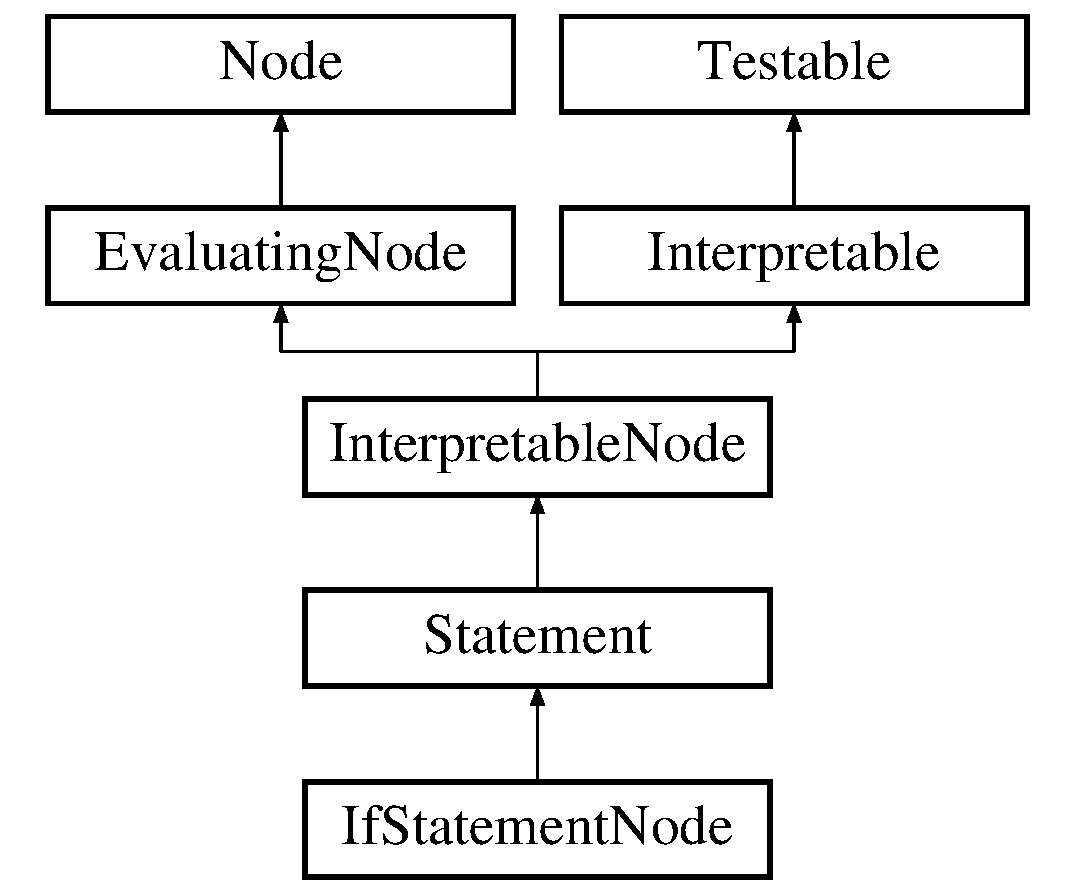
\includegraphics[height=5.000000cm]{classIfStatementNode}
\end{center}
\end{figure}
\subsection*{Public Member Functions}
\begin{DoxyCompactItemize}
\item 
\hyperlink{classIfStatementNode_a99188e8333e6d12e816bd5ba319a7da8}{If\+Statement\+Node} ()
\item 
virtual \hyperlink{classIfStatementNode_a81885b8c46c006ff58324e9121e0bab2}{$\sim$\+If\+Statement\+Node} ()
\item 
virtual \hyperlink{classValue}{Value} \hyperlink{classIfStatementNode_aef627f32330e55f8bb9e5ac2f2f5f3f8}{interpret} (\hyperlink{classInterpreter}{Interpreter} $\ast$interpreter)
\end{DoxyCompactItemize}
\subsection*{Public Attributes}
\begin{DoxyCompactItemize}
\item 
\hyperlink{classExpressionInterpretableNode}{Expression\+Interpretable\+Node} $\ast$ \hyperlink{classIfStatementNode_a021cd8dd0edd333f98d74cfd1c38acd0}{exp}
\end{DoxyCompactItemize}
\subsection*{Additional Inherited Members}


\subsection{Constructor \& Destructor Documentation}
\mbox{\Hypertarget{classIfStatementNode_a99188e8333e6d12e816bd5ba319a7da8}\label{classIfStatementNode_a99188e8333e6d12e816bd5ba319a7da8}} 
\index{If\+Statement\+Node@{If\+Statement\+Node}!If\+Statement\+Node@{If\+Statement\+Node}}
\index{If\+Statement\+Node@{If\+Statement\+Node}!If\+Statement\+Node@{If\+Statement\+Node}}
\subsubsection{\texorpdfstring{If\+Statement\+Node()}{IfStatementNode()}}
{\footnotesize\ttfamily If\+Statement\+Node\+::\+If\+Statement\+Node (\begin{DoxyParamCaption}{ }\end{DoxyParamCaption})}

\mbox{\Hypertarget{classIfStatementNode_a81885b8c46c006ff58324e9121e0bab2}\label{classIfStatementNode_a81885b8c46c006ff58324e9121e0bab2}} 
\index{If\+Statement\+Node@{If\+Statement\+Node}!````~If\+Statement\+Node@{$\sim$\+If\+Statement\+Node}}
\index{````~If\+Statement\+Node@{$\sim$\+If\+Statement\+Node}!If\+Statement\+Node@{If\+Statement\+Node}}
\subsubsection{\texorpdfstring{$\sim$\+If\+Statement\+Node()}{~IfStatementNode()}}
{\footnotesize\ttfamily virtual If\+Statement\+Node\+::$\sim$\+If\+Statement\+Node (\begin{DoxyParamCaption}{ }\end{DoxyParamCaption})\hspace{0.3cm}{\ttfamily [virtual]}}



\subsection{Member Function Documentation}
\mbox{\Hypertarget{classIfStatementNode_aef627f32330e55f8bb9e5ac2f2f5f3f8}\label{classIfStatementNode_aef627f32330e55f8bb9e5ac2f2f5f3f8}} 
\index{If\+Statement\+Node@{If\+Statement\+Node}!interpret@{interpret}}
\index{interpret@{interpret}!If\+Statement\+Node@{If\+Statement\+Node}}
\subsubsection{\texorpdfstring{interpret()}{interpret()}}
{\footnotesize\ttfamily virtual \hyperlink{classValue}{Value} If\+Statement\+Node\+::interpret (\begin{DoxyParamCaption}\item[{\hyperlink{classInterpreter}{Interpreter} $\ast$}]{interpreter }\end{DoxyParamCaption})\hspace{0.3cm}{\ttfamily [virtual]}}



Implements \hyperlink{classInterpretableNode_a9a466e7d65c4b323d2b96b4ac8396cd7}{Interpretable\+Node}.



\subsection{Member Data Documentation}
\mbox{\Hypertarget{classIfStatementNode_a021cd8dd0edd333f98d74cfd1c38acd0}\label{classIfStatementNode_a021cd8dd0edd333f98d74cfd1c38acd0}} 
\index{If\+Statement\+Node@{If\+Statement\+Node}!exp@{exp}}
\index{exp@{exp}!If\+Statement\+Node@{If\+Statement\+Node}}
\subsubsection{\texorpdfstring{exp}{exp}}
{\footnotesize\ttfamily \hyperlink{classExpressionInterpretableNode}{Expression\+Interpretable\+Node}$\ast$ If\+Statement\+Node\+::exp}



The documentation for this class was generated from the following file\+:\begin{DoxyCompactItemize}
\item 
include/\hyperlink{ifstmtnode_8h}{ifstmtnode.\+h}\end{DoxyCompactItemize}

\hypertarget{classInterpretable}{}\section{Interpretable Class Reference}
\label{classInterpretable}\index{Interpretable@{Interpretable}}


{\ttfamily \#include $<$interpretable.\+h$>$}

Inheritance diagram for Interpretable\+:\begin{figure}[H]
\begin{center}
\leavevmode
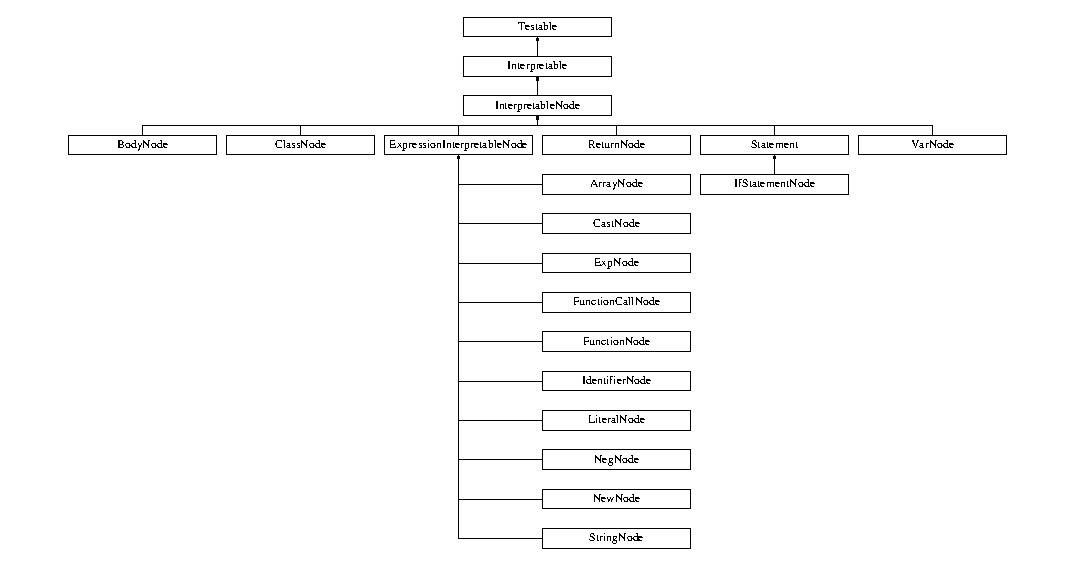
\includegraphics[height=7.140255cm]{classInterpretable}
\end{center}
\end{figure}
\subsection*{Public Member Functions}
\begin{DoxyCompactItemize}
\item 
virtual void \hyperlink{classInterpretable_a32f547aaf68dcbab993284d3257ab010}{test} (\hyperlink{classValidator}{Validator} $\ast$validator)
\item 
virtual \hyperlink{classValue}{Value} \hyperlink{classInterpretable_aa4503765d6dbd00bff7beda913f112ee}{interpret} (\hyperlink{classInterpreter}{Interpreter} $\ast$interpreter)=0
\end{DoxyCompactItemize}


\subsection{Member Function Documentation}
\mbox{\Hypertarget{classInterpretable_aa4503765d6dbd00bff7beda913f112ee}\label{classInterpretable_aa4503765d6dbd00bff7beda913f112ee}} 
\index{Interpretable@{Interpretable}!interpret@{interpret}}
\index{interpret@{interpret}!Interpretable@{Interpretable}}
\subsubsection{\texorpdfstring{interpret()}{interpret()}}
{\footnotesize\ttfamily virtual \hyperlink{classValue}{Value} Interpretable\+::interpret (\begin{DoxyParamCaption}\item[{\hyperlink{classInterpreter}{Interpreter} $\ast$}]{interpreter }\end{DoxyParamCaption})\hspace{0.3cm}{\ttfamily [pure virtual]}}



Implemented in \hyperlink{classNewNode_a77447b9402f0153401bf0e623b5f1e6e}{New\+Node}, \hyperlink{classVarNode_af2eed4fcade96d174c5b1f623b6bcdf6}{Var\+Node}, \hyperlink{classFunctionCallNode_a1d0d8806b7dd501ed43da58f77f7c49e}{Function\+Call\+Node}, \hyperlink{classFunctionNode_a059e6682cd51d0e126372a7af257ea5a}{Function\+Node}, \hyperlink{classExpNode_aedff3b19b9e36a77e4558a168b81debf}{Exp\+Node}, \hyperlink{classBodyNode_a5ab94984d059dba1f7d2baa6022712ba}{Body\+Node}, \hyperlink{classLiteralNode_abb32ed943c6a5b2029a496ac04885b2a}{Literal\+Node}, \hyperlink{classArrayNode_a029220b946233e22cb661fcfac9634d0}{Array\+Node}, \hyperlink{classCastNode_a2a909a7531791bcbc53c514a01ce5024}{Cast\+Node}, \hyperlink{classClassNode_a7515421face64d74e99e180fb297684b}{Class\+Node}, \hyperlink{classIdentifierNode_aa7be7da3e018352f8b549fcac3a8155a}{Identifier\+Node}, \hyperlink{classInterpretableNode_a9a466e7d65c4b323d2b96b4ac8396cd7}{Interpretable\+Node}, \hyperlink{classNegNode_a35ff48d55ab355e27f33dcc21483e4c7}{Neg\+Node}, \hyperlink{classStringNode_ae92c0858cd07baf0c6417f7bdfce9f0d}{String\+Node}, \hyperlink{classExpressionInterpretableNode_a43650f046c48fc539f77a207e3c9181e}{Expression\+Interpretable\+Node}, \hyperlink{classIfStatementNode_aef627f32330e55f8bb9e5ac2f2f5f3f8}{If\+Statement\+Node}, and \hyperlink{classReturnNode_ae6c35829787a4f880b3ee1fa4b2e98d3}{Return\+Node}.

\mbox{\Hypertarget{classInterpretable_a32f547aaf68dcbab993284d3257ab010}\label{classInterpretable_a32f547aaf68dcbab993284d3257ab010}} 
\index{Interpretable@{Interpretable}!test@{test}}
\index{test@{test}!Interpretable@{Interpretable}}
\subsubsection{\texorpdfstring{test()}{test()}}
{\footnotesize\ttfamily virtual void Interpretable\+::test (\begin{DoxyParamCaption}\item[{\hyperlink{classValidator}{Validator} $\ast$}]{validator }\end{DoxyParamCaption})\hspace{0.3cm}{\ttfamily [inline]}, {\ttfamily [virtual]}}



Implements \hyperlink{classTestable_aa10ae4ed84c5d9b36bd69be37790e6ba}{Testable}.



Reimplemented in \hyperlink{classNewNode_a9be504d069e8a5d4ea13b4767a3c792a}{New\+Node}, \hyperlink{classVarNode_afaca674319775ae5e8a4fb0e5ec7b59f}{Var\+Node}, \hyperlink{classExpNode_a8fb8302d5ce438a9ad0f58161be2a1c9}{Exp\+Node}, \hyperlink{classFunctionCallNode_a5a7f576984942e2e39057d716d8a5547}{Function\+Call\+Node}, \hyperlink{classFunctionNode_a1f020e7ea0181b3ce16ad2ef8426f773}{Function\+Node}, \hyperlink{classCastNode_a19fa03c324a6dcbadac32965a86afb3e}{Cast\+Node}, \hyperlink{classBodyNode_a80e75b0ab6c388c34a82bdce63fdc7bb}{Body\+Node}, \hyperlink{classClassNode_ac5147024d81a0c6841e9453025e4f988}{Class\+Node}, \hyperlink{classIdentifierNode_a1459965d8f22ade30cb78b2a1d60dd07}{Identifier\+Node}, \hyperlink{classLiteralNode_af55e4e5e668c9be666c0b6c24c3918f9}{Literal\+Node}, and \hyperlink{classStringNode_a3836ad2a1bb6f86cd52663653a65bad8}{String\+Node}.



The documentation for this class was generated from the following file\+:\begin{DoxyCompactItemize}
\item 
include/\hyperlink{interpretable_8h}{interpretable.\+h}\end{DoxyCompactItemize}

\hypertarget{classInterpretableNode}{}\section{Interpretable\+Node Class Reference}
\label{classInterpretableNode}\index{Interpretable\+Node@{Interpretable\+Node}}


{\ttfamily \#include $<$inode.\+h$>$}

Inheritance diagram for Interpretable\+Node\+:\begin{figure}[H]
\begin{center}
\leavevmode
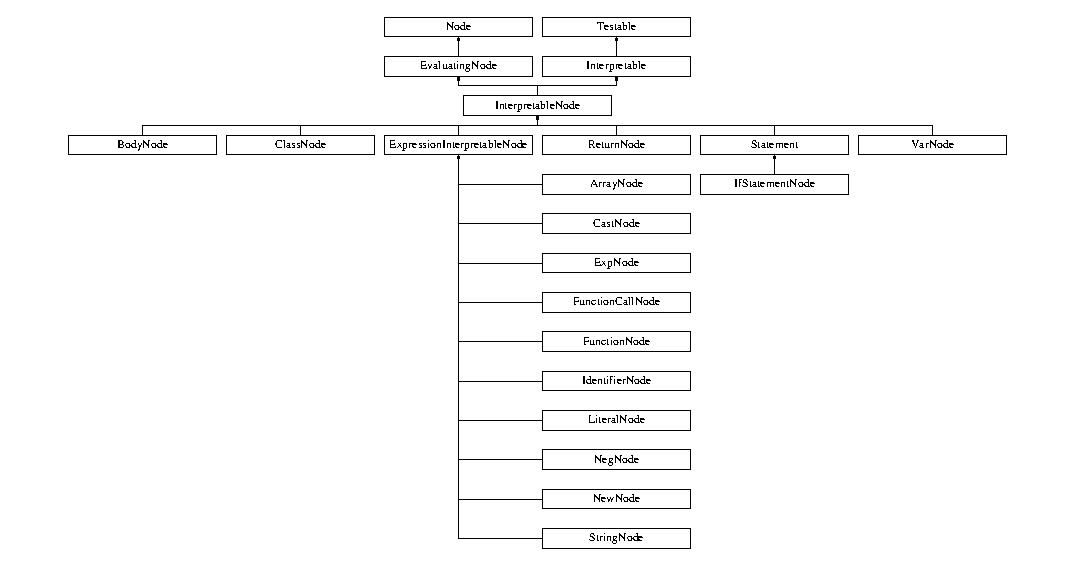
\includegraphics[height=7.140255cm]{classInterpretableNode}
\end{center}
\end{figure}
\subsection*{Public Member Functions}
\begin{DoxyCompactItemize}
\item 
\hyperlink{classInterpretableNode_aeaf40b6165fe9810943c24f7037e03c1}{Interpretable\+Node} (int \hyperlink{classNode_af4f536b1b3f60e197fe364ba56022291}{type})
\item 
virtual \hyperlink{classInterpretableNode_a36f9960c9cfe7267fc518bd5e5462e2e}{$\sim$\+Interpretable\+Node} ()
\item 
virtual \hyperlink{classValue}{Value} \hyperlink{classInterpretableNode_a9a466e7d65c4b323d2b96b4ac8396cd7}{interpret} (\hyperlink{classInterpreter}{Interpreter} $\ast$interpreter)=0
\end{DoxyCompactItemize}
\subsection*{Additional Inherited Members}


\subsection{Constructor \& Destructor Documentation}
\mbox{\Hypertarget{classInterpretableNode_aeaf40b6165fe9810943c24f7037e03c1}\label{classInterpretableNode_aeaf40b6165fe9810943c24f7037e03c1}} 
\index{Interpretable\+Node@{Interpretable\+Node}!Interpretable\+Node@{Interpretable\+Node}}
\index{Interpretable\+Node@{Interpretable\+Node}!Interpretable\+Node@{Interpretable\+Node}}
\subsubsection{\texorpdfstring{Interpretable\+Node()}{InterpretableNode()}}
{\footnotesize\ttfamily Interpretable\+Node\+::\+Interpretable\+Node (\begin{DoxyParamCaption}\item[{int}]{type }\end{DoxyParamCaption})}

\mbox{\Hypertarget{classInterpretableNode_a36f9960c9cfe7267fc518bd5e5462e2e}\label{classInterpretableNode_a36f9960c9cfe7267fc518bd5e5462e2e}} 
\index{Interpretable\+Node@{Interpretable\+Node}!````~Interpretable\+Node@{$\sim$\+Interpretable\+Node}}
\index{````~Interpretable\+Node@{$\sim$\+Interpretable\+Node}!Interpretable\+Node@{Interpretable\+Node}}
\subsubsection{\texorpdfstring{$\sim$\+Interpretable\+Node()}{~InterpretableNode()}}
{\footnotesize\ttfamily virtual Interpretable\+Node\+::$\sim$\+Interpretable\+Node (\begin{DoxyParamCaption}{ }\end{DoxyParamCaption})\hspace{0.3cm}{\ttfamily [virtual]}}



\subsection{Member Function Documentation}
\mbox{\Hypertarget{classInterpretableNode_a9a466e7d65c4b323d2b96b4ac8396cd7}\label{classInterpretableNode_a9a466e7d65c4b323d2b96b4ac8396cd7}} 
\index{Interpretable\+Node@{Interpretable\+Node}!interpret@{interpret}}
\index{interpret@{interpret}!Interpretable\+Node@{Interpretable\+Node}}
\subsubsection{\texorpdfstring{interpret()}{interpret()}}
{\footnotesize\ttfamily virtual \hyperlink{classValue}{Value} Interpretable\+Node\+::interpret (\begin{DoxyParamCaption}\item[{\hyperlink{classInterpreter}{Interpreter} $\ast$}]{interpreter }\end{DoxyParamCaption})\hspace{0.3cm}{\ttfamily [pure virtual]}}



Implements \hyperlink{classInterpretable_aa4503765d6dbd00bff7beda913f112ee}{Interpretable}.



Implemented in \hyperlink{classNewNode_a77447b9402f0153401bf0e623b5f1e6e}{New\+Node}, \hyperlink{classVarNode_af2eed4fcade96d174c5b1f623b6bcdf6}{Var\+Node}, \hyperlink{classFunctionCallNode_a1d0d8806b7dd501ed43da58f77f7c49e}{Function\+Call\+Node}, \hyperlink{classFunctionNode_a059e6682cd51d0e126372a7af257ea5a}{Function\+Node}, \hyperlink{classExpNode_aedff3b19b9e36a77e4558a168b81debf}{Exp\+Node}, \hyperlink{classBodyNode_a5ab94984d059dba1f7d2baa6022712ba}{Body\+Node}, \hyperlink{classLiteralNode_abb32ed943c6a5b2029a496ac04885b2a}{Literal\+Node}, \hyperlink{classArrayNode_a029220b946233e22cb661fcfac9634d0}{Array\+Node}, \hyperlink{classCastNode_a2a909a7531791bcbc53c514a01ce5024}{Cast\+Node}, \hyperlink{classClassNode_a7515421face64d74e99e180fb297684b}{Class\+Node}, \hyperlink{classIdentifierNode_aa7be7da3e018352f8b549fcac3a8155a}{Identifier\+Node}, \hyperlink{classNegNode_a35ff48d55ab355e27f33dcc21483e4c7}{Neg\+Node}, \hyperlink{classStringNode_ae92c0858cd07baf0c6417f7bdfce9f0d}{String\+Node}, \hyperlink{classExpressionInterpretableNode_a43650f046c48fc539f77a207e3c9181e}{Expression\+Interpretable\+Node}, \hyperlink{classIfStatementNode_aef627f32330e55f8bb9e5ac2f2f5f3f8}{If\+Statement\+Node}, and \hyperlink{classReturnNode_ae6c35829787a4f880b3ee1fa4b2e98d3}{Return\+Node}.



The documentation for this class was generated from the following file\+:\begin{DoxyCompactItemize}
\item 
include/\hyperlink{inode_8h}{inode.\+h}\end{DoxyCompactItemize}

\hypertarget{classInterpreter}{}\section{Interpreter Class Reference}
\label{classInterpreter}\index{Interpreter@{Interpreter}}


{\ttfamily \#include $<$interpreter.\+h$>$}

Inheritance diagram for Interpreter\+:\begin{figure}[H]
\begin{center}
\leavevmode
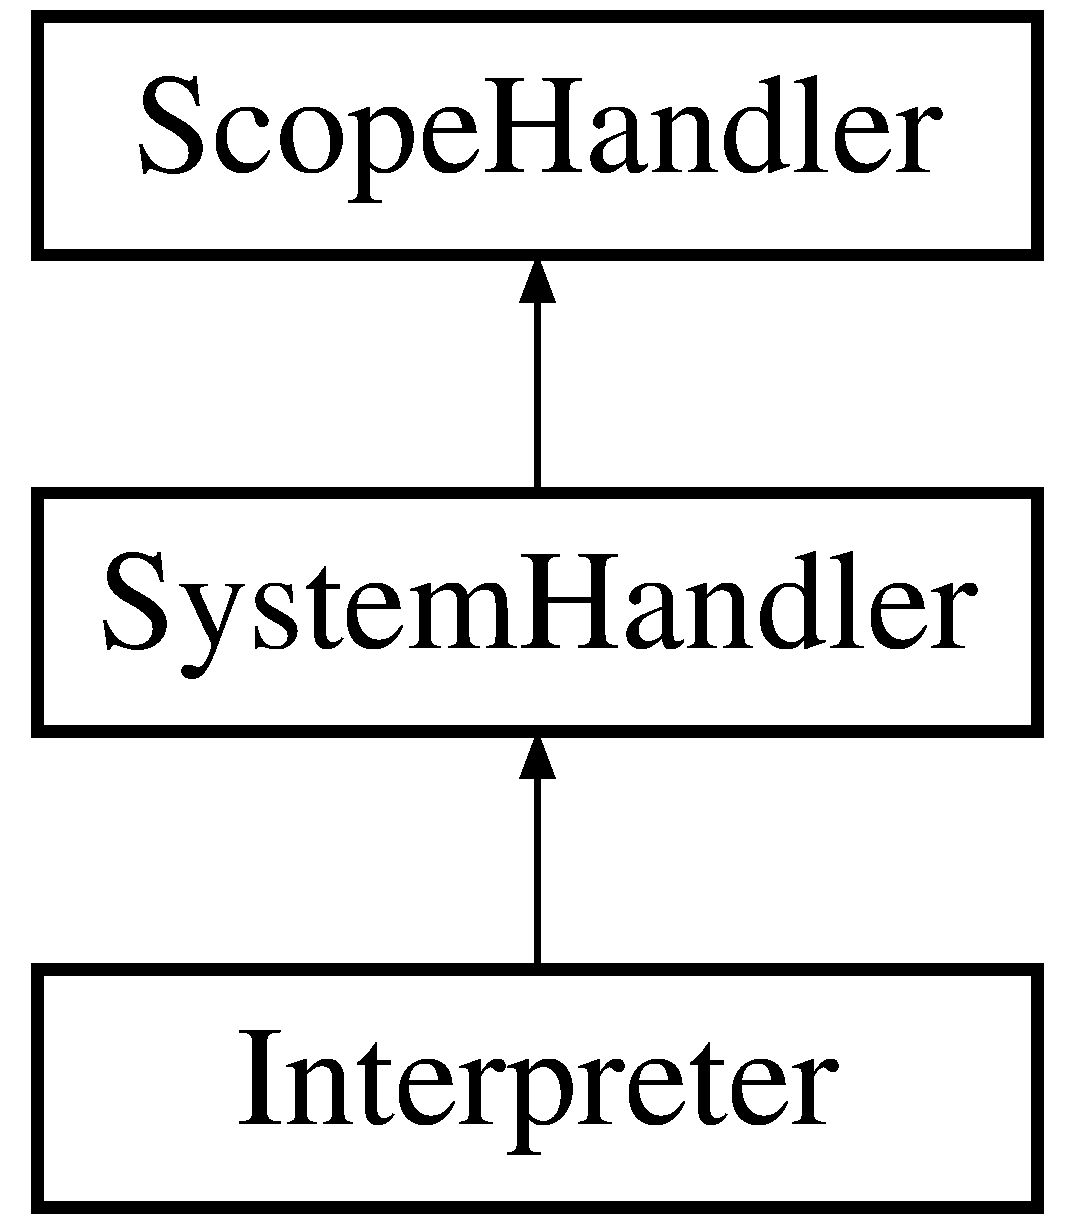
\includegraphics[height=3.000000cm]{classInterpreter}
\end{center}
\end{figure}
\subsection*{Public Member Functions}
\begin{DoxyCompactItemize}
\item 
\hyperlink{classInterpreter_af4a885b059b6af440882047e8406bc9c}{Interpreter} (\hyperlink{classClassSystem}{Class\+System} $\ast$\hyperlink{classSystemHandler_ace6de39b5621a138654577c93f3ce9aa}{class\+System}, \hyperlink{classFunctionSystem}{Function\+System} $\ast$\hyperlink{classSystemHandler_af601707ec9f56e24be4c0541a1c760f4}{base\+Function\+System})
\item 
virtual \hyperlink{classInterpreter_a462a2467300903e0188ac6e4a6a612f6}{$\sim$\+Interpreter} ()
\item 
void \hyperlink{classInterpreter_a3578606fb7dfe1705aee148a468a39a6}{set\+Output\+Function} (\hyperlink{interpreter_8h_a57e80eaa218fd4f66b1d55c833119967}{O\+U\+T\+P\+U\+T\+\_\+\+F\+U\+N\+C\+T\+I\+ON} output)
\item 
void \hyperlink{classInterpreter_ab51bbc767ecf73aca9137b1a78406e20}{ready} ()
\item 
void \hyperlink{classInterpreter_acd0f2550080bcf9c769da5e9b056d005}{run} (const char $\ast$code, \hyperlink{classPosInfo}{Pos\+Info} pos\+Info)
\item 
void \hyperlink{classInterpreter_a98b6ecfea24f94e180bd1853a39f0a12}{run\+Script} (const char $\ast$filename)
\end{DoxyCompactItemize}
\subsection*{Additional Inherited Members}


\subsection{Constructor \& Destructor Documentation}
\mbox{\Hypertarget{classInterpreter_af4a885b059b6af440882047e8406bc9c}\label{classInterpreter_af4a885b059b6af440882047e8406bc9c}} 
\index{Interpreter@{Interpreter}!Interpreter@{Interpreter}}
\index{Interpreter@{Interpreter}!Interpreter@{Interpreter}}
\subsubsection{\texorpdfstring{Interpreter()}{Interpreter()}}
{\footnotesize\ttfamily Interpreter\+::\+Interpreter (\begin{DoxyParamCaption}\item[{\hyperlink{classClassSystem}{Class\+System} $\ast$}]{class\+System,  }\item[{\hyperlink{classFunctionSystem}{Function\+System} $\ast$}]{base\+Function\+System }\end{DoxyParamCaption})}

\mbox{\Hypertarget{classInterpreter_a462a2467300903e0188ac6e4a6a612f6}\label{classInterpreter_a462a2467300903e0188ac6e4a6a612f6}} 
\index{Interpreter@{Interpreter}!````~Interpreter@{$\sim$\+Interpreter}}
\index{````~Interpreter@{$\sim$\+Interpreter}!Interpreter@{Interpreter}}
\subsubsection{\texorpdfstring{$\sim$\+Interpreter()}{~Interpreter()}}
{\footnotesize\ttfamily virtual Interpreter\+::$\sim$\+Interpreter (\begin{DoxyParamCaption}{ }\end{DoxyParamCaption})\hspace{0.3cm}{\ttfamily [virtual]}}



\subsection{Member Function Documentation}
\mbox{\Hypertarget{classInterpreter_ab51bbc767ecf73aca9137b1a78406e20}\label{classInterpreter_ab51bbc767ecf73aca9137b1a78406e20}} 
\index{Interpreter@{Interpreter}!ready@{ready}}
\index{ready@{ready}!Interpreter@{Interpreter}}
\subsubsection{\texorpdfstring{ready()}{ready()}}
{\footnotesize\ttfamily void Interpreter\+::ready (\begin{DoxyParamCaption}{ }\end{DoxyParamCaption})}

\mbox{\Hypertarget{classInterpreter_acd0f2550080bcf9c769da5e9b056d005}\label{classInterpreter_acd0f2550080bcf9c769da5e9b056d005}} 
\index{Interpreter@{Interpreter}!run@{run}}
\index{run@{run}!Interpreter@{Interpreter}}
\subsubsection{\texorpdfstring{run()}{run()}}
{\footnotesize\ttfamily void Interpreter\+::run (\begin{DoxyParamCaption}\item[{const char $\ast$}]{code,  }\item[{\hyperlink{classPosInfo}{Pos\+Info}}]{pos\+Info }\end{DoxyParamCaption})}

\mbox{\Hypertarget{classInterpreter_a98b6ecfea24f94e180bd1853a39f0a12}\label{classInterpreter_a98b6ecfea24f94e180bd1853a39f0a12}} 
\index{Interpreter@{Interpreter}!run\+Script@{run\+Script}}
\index{run\+Script@{run\+Script}!Interpreter@{Interpreter}}
\subsubsection{\texorpdfstring{run\+Script()}{runScript()}}
{\footnotesize\ttfamily void Interpreter\+::run\+Script (\begin{DoxyParamCaption}\item[{const char $\ast$}]{filename }\end{DoxyParamCaption})}

\mbox{\Hypertarget{classInterpreter_a3578606fb7dfe1705aee148a468a39a6}\label{classInterpreter_a3578606fb7dfe1705aee148a468a39a6}} 
\index{Interpreter@{Interpreter}!set\+Output\+Function@{set\+Output\+Function}}
\index{set\+Output\+Function@{set\+Output\+Function}!Interpreter@{Interpreter}}
\subsubsection{\texorpdfstring{set\+Output\+Function()}{setOutputFunction()}}
{\footnotesize\ttfamily void Interpreter\+::set\+Output\+Function (\begin{DoxyParamCaption}\item[{\hyperlink{interpreter_8h_a57e80eaa218fd4f66b1d55c833119967}{O\+U\+T\+P\+U\+T\+\_\+\+F\+U\+N\+C\+T\+I\+ON}}]{output }\end{DoxyParamCaption})}



The documentation for this class was generated from the following file\+:\begin{DoxyCompactItemize}
\item 
include/\hyperlink{interpreter_8h}{interpreter.\+h}\end{DoxyCompactItemize}

\hypertarget{classKeywordNode}{}\section{Keyword\+Node Class Reference}
\label{classKeywordNode}\index{Keyword\+Node@{Keyword\+Node}}


{\ttfamily \#include $<$keywordnode.\+h$>$}

Inheritance diagram for Keyword\+Node\+:\begin{figure}[H]
\begin{center}
\leavevmode
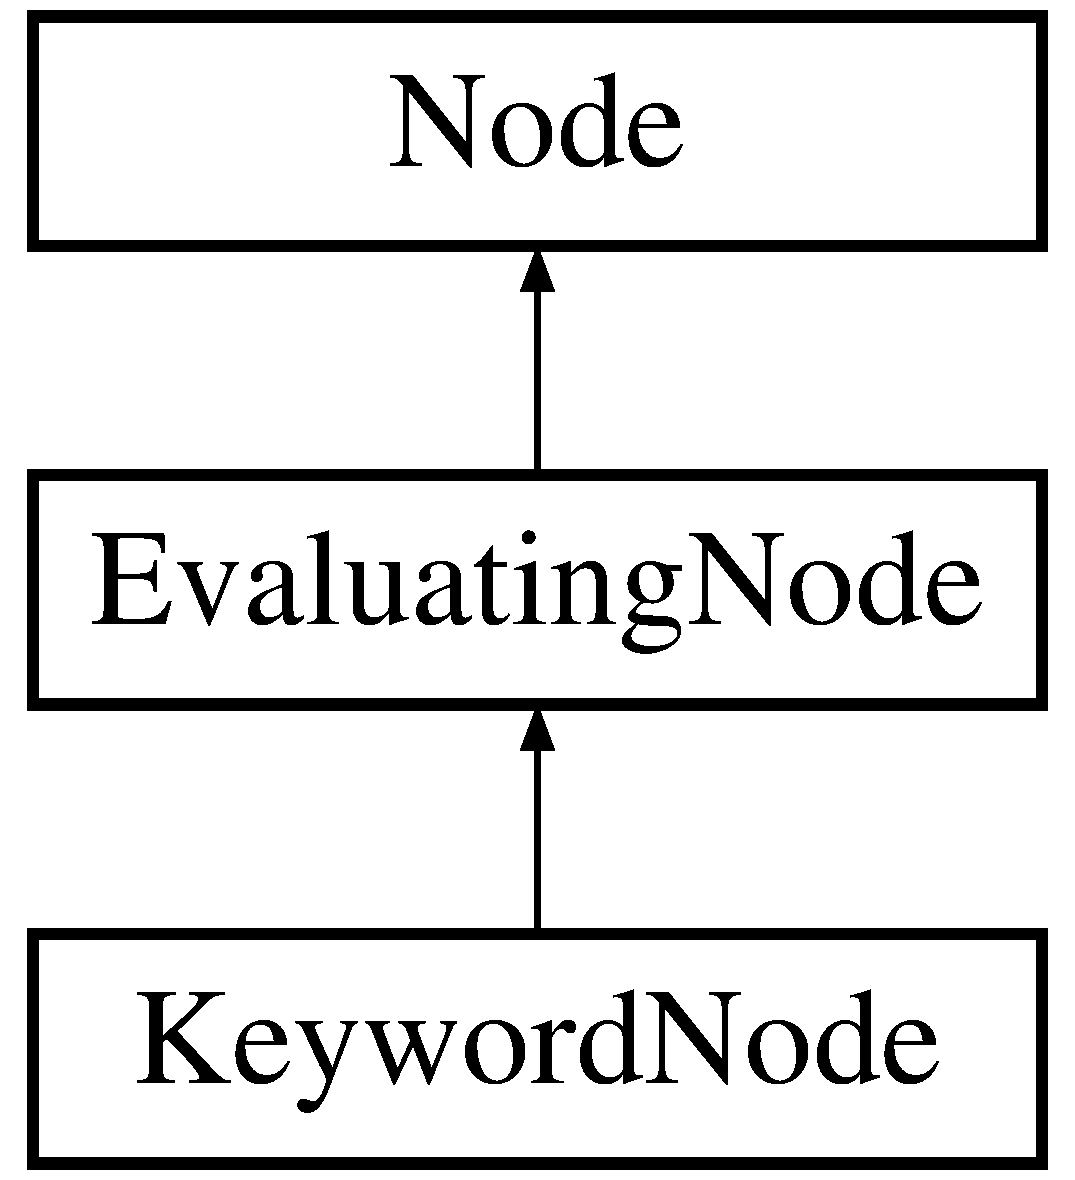
\includegraphics[height=3.000000cm]{classKeywordNode}
\end{center}
\end{figure}
\subsection*{Public Member Functions}
\begin{DoxyCompactItemize}
\item 
\hyperlink{classKeywordNode_ab060b7ee55f027750ad1643036845bc9}{Keyword\+Node} ()
\item 
virtual \hyperlink{classKeywordNode_aecea61e123e74d669b42d009a8dacade}{$\sim$\+Keyword\+Node} ()
\item 
bool \hyperlink{classKeywordNode_a89ea6cb927bd569214b97ba0dff1ebec}{is\+Data\+Type\+Keyword} ()
\item 
virtual void \hyperlink{classKeywordNode_a699f7171c8415901b1a501f72933cfdf}{evaluate\+\_\+impl} (\hyperlink{classSystemHandler}{System\+Handler} $\ast$handler, \hyperlink{statics_8h_a6664c451ca7787483a7981cc1de68dbb}{E\+V\+A\+L\+U\+A\+T\+I\+O\+N\+\_\+\+T\+Y\+PE} expected\+\_\+evaluation, struct \hyperlink{structEvaluation}{Evaluation} $\ast$evaluation)
\end{DoxyCompactItemize}
\subsection*{Public Attributes}
\begin{DoxyCompactItemize}
\item 
std\+::string \hyperlink{classKeywordNode_aa70b672a2e216e214c595ee196f225ae}{value}
\end{DoxyCompactItemize}
\subsection*{Additional Inherited Members}


\subsection{Constructor \& Destructor Documentation}
\mbox{\Hypertarget{classKeywordNode_ab060b7ee55f027750ad1643036845bc9}\label{classKeywordNode_ab060b7ee55f027750ad1643036845bc9}} 
\index{Keyword\+Node@{Keyword\+Node}!Keyword\+Node@{Keyword\+Node}}
\index{Keyword\+Node@{Keyword\+Node}!Keyword\+Node@{Keyword\+Node}}
\subsubsection{\texorpdfstring{Keyword\+Node()}{KeywordNode()}}
{\footnotesize\ttfamily Keyword\+Node\+::\+Keyword\+Node (\begin{DoxyParamCaption}{ }\end{DoxyParamCaption})}

\mbox{\Hypertarget{classKeywordNode_aecea61e123e74d669b42d009a8dacade}\label{classKeywordNode_aecea61e123e74d669b42d009a8dacade}} 
\index{Keyword\+Node@{Keyword\+Node}!````~Keyword\+Node@{$\sim$\+Keyword\+Node}}
\index{````~Keyword\+Node@{$\sim$\+Keyword\+Node}!Keyword\+Node@{Keyword\+Node}}
\subsubsection{\texorpdfstring{$\sim$\+Keyword\+Node()}{~KeywordNode()}}
{\footnotesize\ttfamily virtual Keyword\+Node\+::$\sim$\+Keyword\+Node (\begin{DoxyParamCaption}{ }\end{DoxyParamCaption})\hspace{0.3cm}{\ttfamily [virtual]}}



\subsection{Member Function Documentation}
\mbox{\Hypertarget{classKeywordNode_a699f7171c8415901b1a501f72933cfdf}\label{classKeywordNode_a699f7171c8415901b1a501f72933cfdf}} 
\index{Keyword\+Node@{Keyword\+Node}!evaluate\+\_\+impl@{evaluate\+\_\+impl}}
\index{evaluate\+\_\+impl@{evaluate\+\_\+impl}!Keyword\+Node@{Keyword\+Node}}
\subsubsection{\texorpdfstring{evaluate\+\_\+impl()}{evaluate\_impl()}}
{\footnotesize\ttfamily virtual void Keyword\+Node\+::evaluate\+\_\+impl (\begin{DoxyParamCaption}\item[{\hyperlink{classSystemHandler}{System\+Handler} $\ast$}]{handler,  }\item[{\hyperlink{statics_8h_a6664c451ca7787483a7981cc1de68dbb}{E\+V\+A\+L\+U\+A\+T\+I\+O\+N\+\_\+\+T\+Y\+PE}}]{expected\+\_\+evaluation,  }\item[{struct \hyperlink{structEvaluation}{Evaluation} $\ast$}]{evaluation }\end{DoxyParamCaption})\hspace{0.3cm}{\ttfamily [virtual]}}



Reimplemented from \hyperlink{classEvaluatingNode_abb86fa7334a5871f959b0633db3b5215}{Evaluating\+Node}.

\mbox{\Hypertarget{classKeywordNode_a89ea6cb927bd569214b97ba0dff1ebec}\label{classKeywordNode_a89ea6cb927bd569214b97ba0dff1ebec}} 
\index{Keyword\+Node@{Keyword\+Node}!is\+Data\+Type\+Keyword@{is\+Data\+Type\+Keyword}}
\index{is\+Data\+Type\+Keyword@{is\+Data\+Type\+Keyword}!Keyword\+Node@{Keyword\+Node}}
\subsubsection{\texorpdfstring{is\+Data\+Type\+Keyword()}{isDataTypeKeyword()}}
{\footnotesize\ttfamily bool Keyword\+Node\+::is\+Data\+Type\+Keyword (\begin{DoxyParamCaption}{ }\end{DoxyParamCaption})}



\subsection{Member Data Documentation}
\mbox{\Hypertarget{classKeywordNode_aa70b672a2e216e214c595ee196f225ae}\label{classKeywordNode_aa70b672a2e216e214c595ee196f225ae}} 
\index{Keyword\+Node@{Keyword\+Node}!value@{value}}
\index{value@{value}!Keyword\+Node@{Keyword\+Node}}
\subsubsection{\texorpdfstring{value}{value}}
{\footnotesize\ttfamily std\+::string Keyword\+Node\+::value}



The documentation for this class was generated from the following file\+:\begin{DoxyCompactItemize}
\item 
include/\hyperlink{keywordnode_8h}{keywordnode.\+h}\end{DoxyCompactItemize}

\hypertarget{classLexer}{}\section{Lexer Class Reference}
\label{classLexer}\index{Lexer@{Lexer}}


{\ttfamily \#include $<$lexer.\+h$>$}

\subsection*{Public Member Functions}
\begin{DoxyCompactItemize}
\item 
\hyperlink{classLexer_a6baa61e0f7eb33bd8a2ca3f95c27ac42}{Lexer} (\hyperlink{classLogger}{Logger} $\ast$logger, \hyperlink{classPosInfo}{Pos\+Info} pos\+Info)
\item 
virtual \hyperlink{classLexer_a30d52b09fc54b92a8ee5bebac1be6cec}{$\sim$\+Lexer} ()
\item 
void \hyperlink{classLexer_aec0b93e8614e2327341c73c2adda68c6}{set\+Input} (const char $\ast$buf, int size)
\item 
\hyperlink{classToken}{Token} $\ast$ \hyperlink{classLexer_ad86200e5fb0cbd86882edf63555ebb08}{lex} ()
\end{DoxyCompactItemize}


\subsection{Constructor \& Destructor Documentation}
\mbox{\Hypertarget{classLexer_a6baa61e0f7eb33bd8a2ca3f95c27ac42}\label{classLexer_a6baa61e0f7eb33bd8a2ca3f95c27ac42}} 
\index{Lexer@{Lexer}!Lexer@{Lexer}}
\index{Lexer@{Lexer}!Lexer@{Lexer}}
\subsubsection{\texorpdfstring{Lexer()}{Lexer()}}
{\footnotesize\ttfamily Lexer\+::\+Lexer (\begin{DoxyParamCaption}\item[{\hyperlink{classLogger}{Logger} $\ast$}]{logger,  }\item[{\hyperlink{classPosInfo}{Pos\+Info}}]{pos\+Info }\end{DoxyParamCaption})}

\mbox{\Hypertarget{classLexer_a30d52b09fc54b92a8ee5bebac1be6cec}\label{classLexer_a30d52b09fc54b92a8ee5bebac1be6cec}} 
\index{Lexer@{Lexer}!````~Lexer@{$\sim$\+Lexer}}
\index{````~Lexer@{$\sim$\+Lexer}!Lexer@{Lexer}}
\subsubsection{\texorpdfstring{$\sim$\+Lexer()}{~Lexer()}}
{\footnotesize\ttfamily virtual Lexer\+::$\sim$\+Lexer (\begin{DoxyParamCaption}{ }\end{DoxyParamCaption})\hspace{0.3cm}{\ttfamily [virtual]}}



\subsection{Member Function Documentation}
\mbox{\Hypertarget{classLexer_ad86200e5fb0cbd86882edf63555ebb08}\label{classLexer_ad86200e5fb0cbd86882edf63555ebb08}} 
\index{Lexer@{Lexer}!lex@{lex}}
\index{lex@{lex}!Lexer@{Lexer}}
\subsubsection{\texorpdfstring{lex()}{lex()}}
{\footnotesize\ttfamily \hyperlink{classToken}{Token}$\ast$ Lexer\+::lex (\begin{DoxyParamCaption}{ }\end{DoxyParamCaption})}

\mbox{\Hypertarget{classLexer_aec0b93e8614e2327341c73c2adda68c6}\label{classLexer_aec0b93e8614e2327341c73c2adda68c6}} 
\index{Lexer@{Lexer}!set\+Input@{set\+Input}}
\index{set\+Input@{set\+Input}!Lexer@{Lexer}}
\subsubsection{\texorpdfstring{set\+Input()}{setInput()}}
{\footnotesize\ttfamily void Lexer\+::set\+Input (\begin{DoxyParamCaption}\item[{const char $\ast$}]{buf,  }\item[{int}]{size }\end{DoxyParamCaption})}



The documentation for this class was generated from the following file\+:\begin{DoxyCompactItemize}
\item 
include/\hyperlink{lexer_8h}{lexer.\+h}\end{DoxyCompactItemize}

\hypertarget{classLiteralNode}{}\section{Literal\+Node Class Reference}
\label{classLiteralNode}\index{Literal\+Node@{Literal\+Node}}


{\ttfamily \#include $<$literalnode.\+h$>$}

Inheritance diagram for Literal\+Node\+:\begin{figure}[H]
\begin{center}
\leavevmode
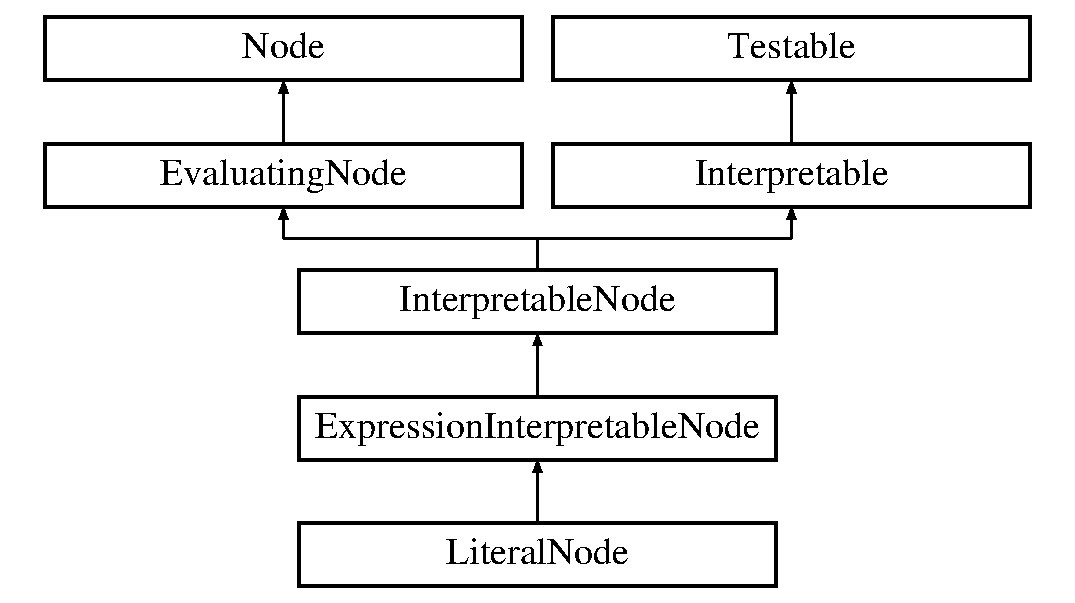
\includegraphics[height=5.000000cm]{classLiteralNode}
\end{center}
\end{figure}
\subsection*{Public Member Functions}
\begin{DoxyCompactItemize}
\item 
\hyperlink{classLiteralNode_ae50674f947b26ee018592984c6c6117b}{Literal\+Node} ()
\item 
virtual \hyperlink{classLiteralNode_a09793ae51506882eaa8d345eeef90d16}{$\sim$\+Literal\+Node} ()
\item 
virtual void \hyperlink{classLiteralNode_af55e4e5e668c9be666c0b6c24c3918f9}{test} (\hyperlink{classValidator}{Validator} $\ast$validator)
\item 
virtual \hyperlink{classValue}{Value} \hyperlink{classLiteralNode_abb32ed943c6a5b2029a496ac04885b2a}{interpret} (\hyperlink{classInterpreter}{Interpreter} $\ast$interpreter)
\item 
virtual void \hyperlink{classLiteralNode_ac468128f093b3955ddd7c85eaa959ec2}{evaluate\+\_\+impl} (\hyperlink{classSystemHandler}{System\+Handler} $\ast$handler, \hyperlink{statics_8h_a6664c451ca7787483a7981cc1de68dbb}{E\+V\+A\+L\+U\+A\+T\+I\+O\+N\+\_\+\+T\+Y\+PE} expected\+\_\+evaluation, struct \hyperlink{structEvaluation}{Evaluation} $\ast$evaluation)
\end{DoxyCompactItemize}
\subsection*{Public Attributes}
\begin{DoxyCompactItemize}
\item 
double \hyperlink{classLiteralNode_aaead85ec08c6a4ec23534a547176a450}{value}
\end{DoxyCompactItemize}
\subsection*{Additional Inherited Members}


\subsection{Constructor \& Destructor Documentation}
\mbox{\Hypertarget{classLiteralNode_ae50674f947b26ee018592984c6c6117b}\label{classLiteralNode_ae50674f947b26ee018592984c6c6117b}} 
\index{Literal\+Node@{Literal\+Node}!Literal\+Node@{Literal\+Node}}
\index{Literal\+Node@{Literal\+Node}!Literal\+Node@{Literal\+Node}}
\subsubsection{\texorpdfstring{Literal\+Node()}{LiteralNode()}}
{\footnotesize\ttfamily Literal\+Node\+::\+Literal\+Node (\begin{DoxyParamCaption}{ }\end{DoxyParamCaption})}

\mbox{\Hypertarget{classLiteralNode_a09793ae51506882eaa8d345eeef90d16}\label{classLiteralNode_a09793ae51506882eaa8d345eeef90d16}} 
\index{Literal\+Node@{Literal\+Node}!````~Literal\+Node@{$\sim$\+Literal\+Node}}
\index{````~Literal\+Node@{$\sim$\+Literal\+Node}!Literal\+Node@{Literal\+Node}}
\subsubsection{\texorpdfstring{$\sim$\+Literal\+Node()}{~LiteralNode()}}
{\footnotesize\ttfamily virtual Literal\+Node\+::$\sim$\+Literal\+Node (\begin{DoxyParamCaption}{ }\end{DoxyParamCaption})\hspace{0.3cm}{\ttfamily [virtual]}}



\subsection{Member Function Documentation}
\mbox{\Hypertarget{classLiteralNode_ac468128f093b3955ddd7c85eaa959ec2}\label{classLiteralNode_ac468128f093b3955ddd7c85eaa959ec2}} 
\index{Literal\+Node@{Literal\+Node}!evaluate\+\_\+impl@{evaluate\+\_\+impl}}
\index{evaluate\+\_\+impl@{evaluate\+\_\+impl}!Literal\+Node@{Literal\+Node}}
\subsubsection{\texorpdfstring{evaluate\+\_\+impl()}{evaluate\_impl()}}
{\footnotesize\ttfamily virtual void Literal\+Node\+::evaluate\+\_\+impl (\begin{DoxyParamCaption}\item[{\hyperlink{classSystemHandler}{System\+Handler} $\ast$}]{handler,  }\item[{\hyperlink{statics_8h_a6664c451ca7787483a7981cc1de68dbb}{E\+V\+A\+L\+U\+A\+T\+I\+O\+N\+\_\+\+T\+Y\+PE}}]{expected\+\_\+evaluation,  }\item[{struct \hyperlink{structEvaluation}{Evaluation} $\ast$}]{evaluation }\end{DoxyParamCaption})\hspace{0.3cm}{\ttfamily [virtual]}}



Implements \hyperlink{classEvaluatingNode_a085fa06e0b46a93c814dc55cda0c1b26}{Evaluating\+Node}.

\mbox{\Hypertarget{classLiteralNode_abb32ed943c6a5b2029a496ac04885b2a}\label{classLiteralNode_abb32ed943c6a5b2029a496ac04885b2a}} 
\index{Literal\+Node@{Literal\+Node}!interpret@{interpret}}
\index{interpret@{interpret}!Literal\+Node@{Literal\+Node}}
\subsubsection{\texorpdfstring{interpret()}{interpret()}}
{\footnotesize\ttfamily virtual \hyperlink{classValue}{Value} Literal\+Node\+::interpret (\begin{DoxyParamCaption}\item[{\hyperlink{classInterpreter}{Interpreter} $\ast$}]{interpreter }\end{DoxyParamCaption})\hspace{0.3cm}{\ttfamily [virtual]}}



Implements \hyperlink{classExpressionInterpretableNode_a43650f046c48fc539f77a207e3c9181e}{Expression\+Interpretable\+Node}.

\mbox{\Hypertarget{classLiteralNode_af55e4e5e668c9be666c0b6c24c3918f9}\label{classLiteralNode_af55e4e5e668c9be666c0b6c24c3918f9}} 
\index{Literal\+Node@{Literal\+Node}!test@{test}}
\index{test@{test}!Literal\+Node@{Literal\+Node}}
\subsubsection{\texorpdfstring{test()}{test()}}
{\footnotesize\ttfamily virtual void Literal\+Node\+::test (\begin{DoxyParamCaption}\item[{\hyperlink{classValidator}{Validator} $\ast$}]{validator }\end{DoxyParamCaption})\hspace{0.3cm}{\ttfamily [virtual]}}



Reimplemented from \hyperlink{classInterpretable_a32f547aaf68dcbab993284d3257ab010}{Interpretable}.



\subsection{Member Data Documentation}
\mbox{\Hypertarget{classLiteralNode_aaead85ec08c6a4ec23534a547176a450}\label{classLiteralNode_aaead85ec08c6a4ec23534a547176a450}} 
\index{Literal\+Node@{Literal\+Node}!value@{value}}
\index{value@{value}!Literal\+Node@{Literal\+Node}}
\subsubsection{\texorpdfstring{value}{value}}
{\footnotesize\ttfamily double Literal\+Node\+::value}



The documentation for this class was generated from the following file\+:\begin{DoxyCompactItemize}
\item 
include/\hyperlink{literalnode_8h}{literalnode.\+h}\end{DoxyCompactItemize}

\hypertarget{classLogEntry}{}\section{Log\+Entry Class Reference}
\label{classLogEntry}\index{Log\+Entry@{Log\+Entry}}


{\ttfamily \#include $<$logger.\+h$>$}

\subsection*{Public Member Functions}
\begin{DoxyCompactItemize}
\item 
\hyperlink{classLogEntry_a02d0d5d77728cf54c92184a645ae8ab8}{Log\+Entry} (int \hyperlink{classLogEntry_a8bb959695c7dfe5eaf19f70fdc3f8a71}{level}, std\+::string \hyperlink{classLogEntry_a7ad3f1e2f6f00453e0c0bafc6ba5dfa8}{message}, \hyperlink{classPosInfo}{Pos\+Info} \hyperlink{classLogEntry_a0918b72d75e039af6a03e743f8615ebc}{pos\+Info})
\item 
virtual \hyperlink{classLogEntry_a835d70a7c0e233eea081c4540b2b959d}{$\sim$\+Log\+Entry} ()
\end{DoxyCompactItemize}
\subsection*{Public Attributes}
\begin{DoxyCompactItemize}
\item 
const int \hyperlink{classLogEntry_a8bb959695c7dfe5eaf19f70fdc3f8a71}{level}
\item 
const std\+::string \hyperlink{classLogEntry_a7ad3f1e2f6f00453e0c0bafc6ba5dfa8}{message}
\item 
const \hyperlink{classPosInfo}{Pos\+Info} \hyperlink{classLogEntry_a0918b72d75e039af6a03e743f8615ebc}{pos\+Info}
\end{DoxyCompactItemize}


\subsection{Constructor \& Destructor Documentation}
\mbox{\Hypertarget{classLogEntry_a02d0d5d77728cf54c92184a645ae8ab8}\label{classLogEntry_a02d0d5d77728cf54c92184a645ae8ab8}} 
\index{Log\+Entry@{Log\+Entry}!Log\+Entry@{Log\+Entry}}
\index{Log\+Entry@{Log\+Entry}!Log\+Entry@{Log\+Entry}}
\subsubsection{\texorpdfstring{Log\+Entry()}{LogEntry()}}
{\footnotesize\ttfamily Log\+Entry\+::\+Log\+Entry (\begin{DoxyParamCaption}\item[{int}]{level,  }\item[{std\+::string}]{message,  }\item[{\hyperlink{classPosInfo}{Pos\+Info}}]{pos\+Info }\end{DoxyParamCaption})}

\mbox{\Hypertarget{classLogEntry_a835d70a7c0e233eea081c4540b2b959d}\label{classLogEntry_a835d70a7c0e233eea081c4540b2b959d}} 
\index{Log\+Entry@{Log\+Entry}!````~Log\+Entry@{$\sim$\+Log\+Entry}}
\index{````~Log\+Entry@{$\sim$\+Log\+Entry}!Log\+Entry@{Log\+Entry}}
\subsubsection{\texorpdfstring{$\sim$\+Log\+Entry()}{~LogEntry()}}
{\footnotesize\ttfamily virtual Log\+Entry\+::$\sim$\+Log\+Entry (\begin{DoxyParamCaption}{ }\end{DoxyParamCaption})\hspace{0.3cm}{\ttfamily [virtual]}}



\subsection{Member Data Documentation}
\mbox{\Hypertarget{classLogEntry_a8bb959695c7dfe5eaf19f70fdc3f8a71}\label{classLogEntry_a8bb959695c7dfe5eaf19f70fdc3f8a71}} 
\index{Log\+Entry@{Log\+Entry}!level@{level}}
\index{level@{level}!Log\+Entry@{Log\+Entry}}
\subsubsection{\texorpdfstring{level}{level}}
{\footnotesize\ttfamily const int Log\+Entry\+::level}

\mbox{\Hypertarget{classLogEntry_a7ad3f1e2f6f00453e0c0bafc6ba5dfa8}\label{classLogEntry_a7ad3f1e2f6f00453e0c0bafc6ba5dfa8}} 
\index{Log\+Entry@{Log\+Entry}!message@{message}}
\index{message@{message}!Log\+Entry@{Log\+Entry}}
\subsubsection{\texorpdfstring{message}{message}}
{\footnotesize\ttfamily const std\+::string Log\+Entry\+::message}

\mbox{\Hypertarget{classLogEntry_a0918b72d75e039af6a03e743f8615ebc}\label{classLogEntry_a0918b72d75e039af6a03e743f8615ebc}} 
\index{Log\+Entry@{Log\+Entry}!pos\+Info@{pos\+Info}}
\index{pos\+Info@{pos\+Info}!Log\+Entry@{Log\+Entry}}
\subsubsection{\texorpdfstring{pos\+Info}{posInfo}}
{\footnotesize\ttfamily const \hyperlink{classPosInfo}{Pos\+Info} Log\+Entry\+::pos\+Info}



The documentation for this class was generated from the following file\+:\begin{DoxyCompactItemize}
\item 
include/\hyperlink{logger_8h}{logger.\+h}\end{DoxyCompactItemize}

\hypertarget{classLogger}{}\section{Logger Class Reference}
\label{classLogger}\index{Logger@{Logger}}


{\ttfamily \#include $<$logger.\+h$>$}

\subsection*{Public Member Functions}
\begin{DoxyCompactItemize}
\item 
\hyperlink{classLogger_abc41bfb031d896170c7675fa96a6b30c}{Logger} ()
\item 
virtual \hyperlink{classLogger_ae93f62ca3e47716b7120acb032a260f3}{$\sim$\+Logger} ()
\item 
void \hyperlink{classLogger_a31d66ebf52bace306ed8a8f0e0b1f516}{warn} (std\+::string message, \hyperlink{classPosInfo}{Pos\+Info} pos\+Info)
\item 
void \hyperlink{classLogger_a63306c62d25e4d514e8485a9566dde22}{error} (std\+::string message, \hyperlink{classPosInfo}{Pos\+Info} pos\+Info)
\item 
bool \hyperlink{classLogger_a261361c60868c98ab4ea4e562842da1f}{has\+Log} ()
\item 
bool \hyperlink{classLogger_a0a52b10db87dc64e9cb8c991162463f9}{has\+Errors} ()
\end{DoxyCompactItemize}
\subsection*{Public Attributes}
\begin{DoxyCompactItemize}
\item 
std\+::vector$<$ \hyperlink{classLogEntry}{Log\+Entry} $>$ \hyperlink{classLogger_a151c8e1606c22b796aa5ed817a1b5a54}{entries}
\end{DoxyCompactItemize}


\subsection{Constructor \& Destructor Documentation}
\mbox{\Hypertarget{classLogger_abc41bfb031d896170c7675fa96a6b30c}\label{classLogger_abc41bfb031d896170c7675fa96a6b30c}} 
\index{Logger@{Logger}!Logger@{Logger}}
\index{Logger@{Logger}!Logger@{Logger}}
\subsubsection{\texorpdfstring{Logger()}{Logger()}}
{\footnotesize\ttfamily Logger\+::\+Logger (\begin{DoxyParamCaption}{ }\end{DoxyParamCaption})}

\mbox{\Hypertarget{classLogger_ae93f62ca3e47716b7120acb032a260f3}\label{classLogger_ae93f62ca3e47716b7120acb032a260f3}} 
\index{Logger@{Logger}!````~Logger@{$\sim$\+Logger}}
\index{````~Logger@{$\sim$\+Logger}!Logger@{Logger}}
\subsubsection{\texorpdfstring{$\sim$\+Logger()}{~Logger()}}
{\footnotesize\ttfamily virtual Logger\+::$\sim$\+Logger (\begin{DoxyParamCaption}{ }\end{DoxyParamCaption})\hspace{0.3cm}{\ttfamily [virtual]}}



\subsection{Member Function Documentation}
\mbox{\Hypertarget{classLogger_a63306c62d25e4d514e8485a9566dde22}\label{classLogger_a63306c62d25e4d514e8485a9566dde22}} 
\index{Logger@{Logger}!error@{error}}
\index{error@{error}!Logger@{Logger}}
\subsubsection{\texorpdfstring{error()}{error()}}
{\footnotesize\ttfamily void Logger\+::error (\begin{DoxyParamCaption}\item[{std\+::string}]{message,  }\item[{\hyperlink{classPosInfo}{Pos\+Info}}]{pos\+Info }\end{DoxyParamCaption})}

\mbox{\Hypertarget{classLogger_a0a52b10db87dc64e9cb8c991162463f9}\label{classLogger_a0a52b10db87dc64e9cb8c991162463f9}} 
\index{Logger@{Logger}!has\+Errors@{has\+Errors}}
\index{has\+Errors@{has\+Errors}!Logger@{Logger}}
\subsubsection{\texorpdfstring{has\+Errors()}{hasErrors()}}
{\footnotesize\ttfamily bool Logger\+::has\+Errors (\begin{DoxyParamCaption}{ }\end{DoxyParamCaption})}

\mbox{\Hypertarget{classLogger_a261361c60868c98ab4ea4e562842da1f}\label{classLogger_a261361c60868c98ab4ea4e562842da1f}} 
\index{Logger@{Logger}!has\+Log@{has\+Log}}
\index{has\+Log@{has\+Log}!Logger@{Logger}}
\subsubsection{\texorpdfstring{has\+Log()}{hasLog()}}
{\footnotesize\ttfamily bool Logger\+::has\+Log (\begin{DoxyParamCaption}{ }\end{DoxyParamCaption})}

\mbox{\Hypertarget{classLogger_a31d66ebf52bace306ed8a8f0e0b1f516}\label{classLogger_a31d66ebf52bace306ed8a8f0e0b1f516}} 
\index{Logger@{Logger}!warn@{warn}}
\index{warn@{warn}!Logger@{Logger}}
\subsubsection{\texorpdfstring{warn()}{warn()}}
{\footnotesize\ttfamily void Logger\+::warn (\begin{DoxyParamCaption}\item[{std\+::string}]{message,  }\item[{\hyperlink{classPosInfo}{Pos\+Info}}]{pos\+Info }\end{DoxyParamCaption})}



\subsection{Member Data Documentation}
\mbox{\Hypertarget{classLogger_a151c8e1606c22b796aa5ed817a1b5a54}\label{classLogger_a151c8e1606c22b796aa5ed817a1b5a54}} 
\index{Logger@{Logger}!entries@{entries}}
\index{entries@{entries}!Logger@{Logger}}
\subsubsection{\texorpdfstring{entries}{entries}}
{\footnotesize\ttfamily std\+::vector$<$\hyperlink{classLogEntry}{Log\+Entry}$>$ Logger\+::entries}



The documentation for this class was generated from the following file\+:\begin{DoxyCompactItemize}
\item 
include/\hyperlink{logger_8h}{logger.\+h}\end{DoxyCompactItemize}

\hypertarget{structmarble__code}{}\section{marble\+\_\+code Struct Reference}
\label{structmarble__code}\index{marble\+\_\+code@{marble\+\_\+code}}


{\ttfamily \#include $<$splitter.\+h$>$}

Inheritance diagram for marble\+\_\+code\+:\begin{figure}[H]
\begin{center}
\leavevmode
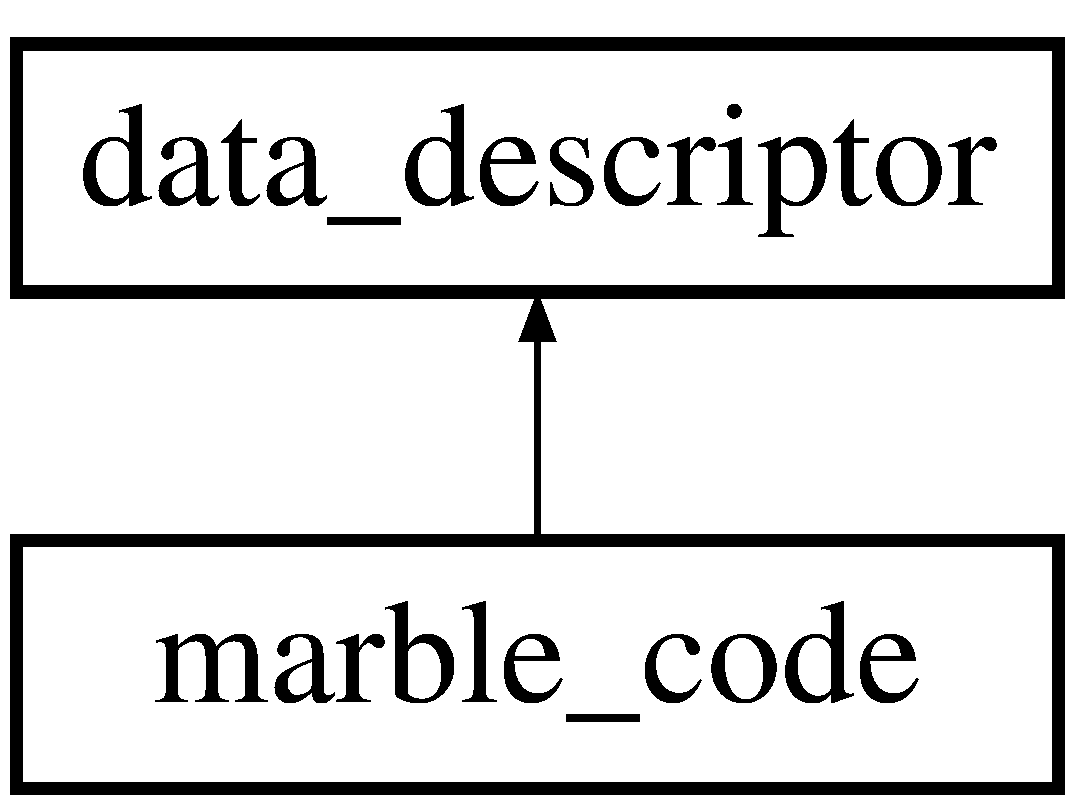
\includegraphics[height=2.000000cm]{structmarble__code}
\end{center}
\end{figure}
\subsection*{Public Member Functions}
\begin{DoxyCompactItemize}
\item 
void \hyperlink{structmarble__code_ac2d593b81e3f340f11e8fe6b8978163b}{update} ()
\end{DoxyCompactItemize}
\subsection*{Additional Inherited Members}


\subsection{Member Function Documentation}
\mbox{\Hypertarget{structmarble__code_ac2d593b81e3f340f11e8fe6b8978163b}\label{structmarble__code_ac2d593b81e3f340f11e8fe6b8978163b}} 
\index{marble\+\_\+code@{marble\+\_\+code}!update@{update}}
\index{update@{update}!marble\+\_\+code@{marble\+\_\+code}}
\subsubsection{\texorpdfstring{update()}{update()}}
{\footnotesize\ttfamily void marble\+\_\+code\+::update (\begin{DoxyParamCaption}{ }\end{DoxyParamCaption})\hspace{0.3cm}{\ttfamily [virtual]}}



Reimplemented from \hyperlink{structdata__descriptor_ad6cd92beb7d2b9291e0d130a24faa380}{data\+\_\+descriptor}.



The documentation for this struct was generated from the following file\+:\begin{DoxyCompactItemize}
\item 
include/\hyperlink{splitter_8h}{splitter.\+h}\end{DoxyCompactItemize}

\hypertarget{classNativeFunction}{}\section{Native\+Function Class Reference}
\label{classNativeFunction}\index{Native\+Function@{Native\+Function}}


{\ttfamily \#include $<$nativefunction.\+h$>$}

Inheritance diagram for Native\+Function\+:\begin{figure}[H]
\begin{center}
\leavevmode
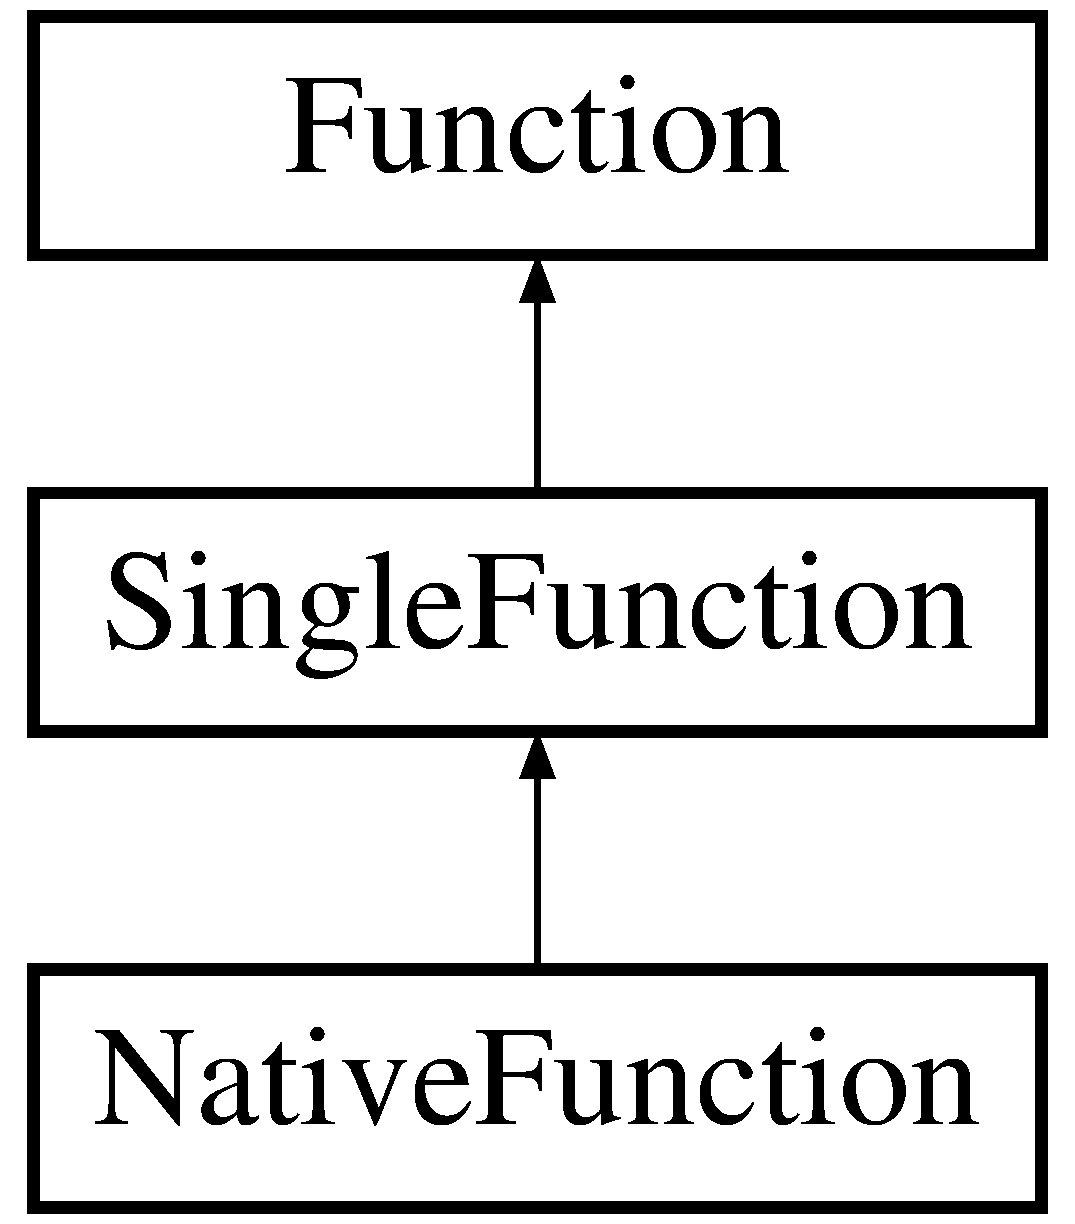
\includegraphics[height=3.000000cm]{classNativeFunction}
\end{center}
\end{figure}
\subsection*{Public Member Functions}
\begin{DoxyCompactItemize}
\item 
\hyperlink{classNativeFunction_a189f9fd9161c741e533c3dc2c8396f31}{Native\+Function} (std\+::string \hyperlink{classFunction_a161d1ceb4f67f3222caf429fea7b71f1}{name}, std\+::vector$<$ \hyperlink{classVarType}{Var\+Type} $>$ \hyperlink{classSingleFunction_a345cc7c6a42587a62495688af6644a26}{argument\+\_\+types}, std\+::function$<$ void(std\+::vector$<$ \hyperlink{classValue}{Value} $>$, \hyperlink{classValue}{Value} $\ast$return\+\_\+value, std\+::shared\+\_\+ptr$<$ \hyperlink{classObject}{Object} $>$ object)$>$ entrypoint)
\item 
virtual \hyperlink{classNativeFunction_aa6055c6a092b8be8d1f9009efc6db0e0}{$\sim$\+Native\+Function} ()
\item 
virtual void \hyperlink{classNativeFunction_a0f003d805cbc3625e311d1b2a1b861d9}{invoke} (std\+::vector$<$ \hyperlink{classValue}{Value} $>$ values, \hyperlink{classValue}{Value} $\ast$return\+\_\+value, std\+::shared\+\_\+ptr$<$ \hyperlink{classObject}{Object} $>$ object)
\end{DoxyCompactItemize}
\subsection*{Additional Inherited Members}


\subsection{Constructor \& Destructor Documentation}
\mbox{\Hypertarget{classNativeFunction_a189f9fd9161c741e533c3dc2c8396f31}\label{classNativeFunction_a189f9fd9161c741e533c3dc2c8396f31}} 
\index{Native\+Function@{Native\+Function}!Native\+Function@{Native\+Function}}
\index{Native\+Function@{Native\+Function}!Native\+Function@{Native\+Function}}
\subsubsection{\texorpdfstring{Native\+Function()}{NativeFunction()}}
{\footnotesize\ttfamily Native\+Function\+::\+Native\+Function (\begin{DoxyParamCaption}\item[{std\+::string}]{name,  }\item[{std\+::vector$<$ \hyperlink{classVarType}{Var\+Type} $>$}]{argument\+\_\+types,  }\item[{std\+::function$<$ void(std\+::vector$<$ \hyperlink{classValue}{Value} $>$, \hyperlink{classValue}{Value} $\ast$return\+\_\+value, std\+::shared\+\_\+ptr$<$ \hyperlink{classObject}{Object} $>$ object)$>$}]{entrypoint }\end{DoxyParamCaption})}

\mbox{\Hypertarget{classNativeFunction_aa6055c6a092b8be8d1f9009efc6db0e0}\label{classNativeFunction_aa6055c6a092b8be8d1f9009efc6db0e0}} 
\index{Native\+Function@{Native\+Function}!````~Native\+Function@{$\sim$\+Native\+Function}}
\index{````~Native\+Function@{$\sim$\+Native\+Function}!Native\+Function@{Native\+Function}}
\subsubsection{\texorpdfstring{$\sim$\+Native\+Function()}{~NativeFunction()}}
{\footnotesize\ttfamily virtual Native\+Function\+::$\sim$\+Native\+Function (\begin{DoxyParamCaption}{ }\end{DoxyParamCaption})\hspace{0.3cm}{\ttfamily [virtual]}}



\subsection{Member Function Documentation}
\mbox{\Hypertarget{classNativeFunction_a0f003d805cbc3625e311d1b2a1b861d9}\label{classNativeFunction_a0f003d805cbc3625e311d1b2a1b861d9}} 
\index{Native\+Function@{Native\+Function}!invoke@{invoke}}
\index{invoke@{invoke}!Native\+Function@{Native\+Function}}
\subsubsection{\texorpdfstring{invoke()}{invoke()}}
{\footnotesize\ttfamily virtual void Native\+Function\+::invoke (\begin{DoxyParamCaption}\item[{std\+::vector$<$ \hyperlink{classValue}{Value} $>$}]{values,  }\item[{\hyperlink{classValue}{Value} $\ast$}]{return\+\_\+value,  }\item[{std\+::shared\+\_\+ptr$<$ \hyperlink{classObject}{Object} $>$}]{object }\end{DoxyParamCaption})\hspace{0.3cm}{\ttfamily [virtual]}}



Implements \hyperlink{classFunction_a84f9a63e68becc27e58ea738ba4cd698}{Function}.



The documentation for this class was generated from the following file\+:\begin{DoxyCompactItemize}
\item 
include/\hyperlink{nativefunction_8h}{nativefunction.\+h}\end{DoxyCompactItemize}

\hypertarget{classNegNode}{}\section{Neg\+Node Class Reference}
\label{classNegNode}\index{Neg\+Node@{Neg\+Node}}


{\ttfamily \#include $<$negnode.\+h$>$}

Inheritance diagram for Neg\+Node\+:\begin{figure}[H]
\begin{center}
\leavevmode
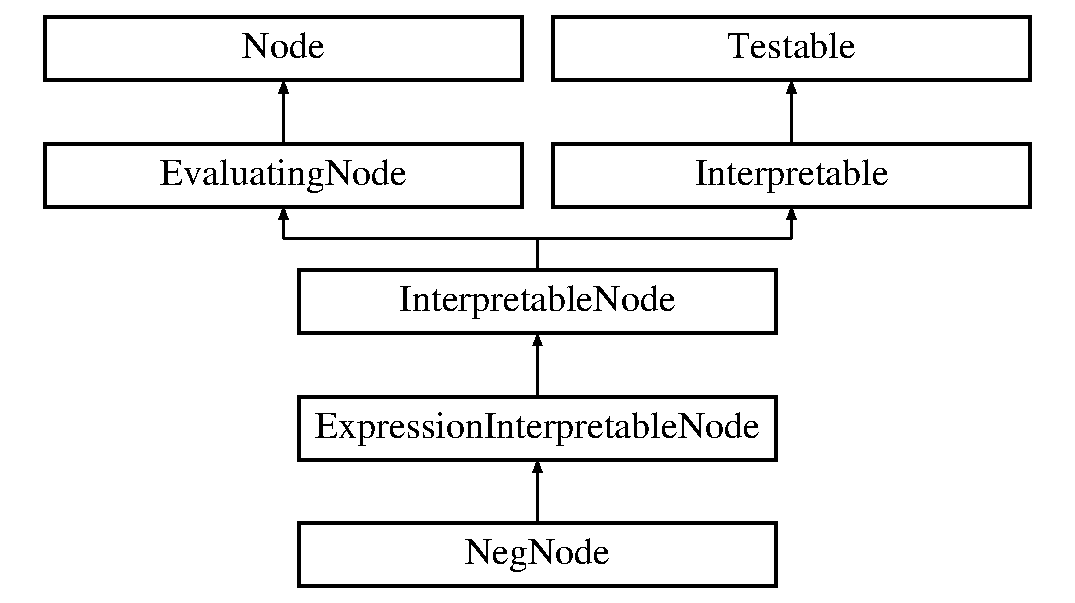
\includegraphics[height=5.000000cm]{classNegNode}
\end{center}
\end{figure}
\subsection*{Public Member Functions}
\begin{DoxyCompactItemize}
\item 
\hyperlink{classNegNode_a543d2b5abde85cbcaca1e8927ec55c9e}{Neg\+Node} ()
\item 
virtual \hyperlink{classNegNode_aba880abbb0e47060985c5ec3e3e0c3fc}{$\sim$\+Neg\+Node} ()
\item 
virtual \hyperlink{classValue}{Value} \hyperlink{classNegNode_a35ff48d55ab355e27f33dcc21483e4c7}{interpret} (\hyperlink{classInterpreter}{Interpreter} $\ast$interpreter)
\end{DoxyCompactItemize}
\subsection*{Public Attributes}
\begin{DoxyCompactItemize}
\item 
\hyperlink{classExpressionInterpretableNode}{Expression\+Interpretable\+Node} $\ast$ \hyperlink{classNegNode_ac1c92a11fc98afbb953cd391d84074c2}{node}
\end{DoxyCompactItemize}
\subsection*{Additional Inherited Members}


\subsection{Constructor \& Destructor Documentation}
\mbox{\Hypertarget{classNegNode_a543d2b5abde85cbcaca1e8927ec55c9e}\label{classNegNode_a543d2b5abde85cbcaca1e8927ec55c9e}} 
\index{Neg\+Node@{Neg\+Node}!Neg\+Node@{Neg\+Node}}
\index{Neg\+Node@{Neg\+Node}!Neg\+Node@{Neg\+Node}}
\subsubsection{\texorpdfstring{Neg\+Node()}{NegNode()}}
{\footnotesize\ttfamily Neg\+Node\+::\+Neg\+Node (\begin{DoxyParamCaption}{ }\end{DoxyParamCaption})}

\mbox{\Hypertarget{classNegNode_aba880abbb0e47060985c5ec3e3e0c3fc}\label{classNegNode_aba880abbb0e47060985c5ec3e3e0c3fc}} 
\index{Neg\+Node@{Neg\+Node}!````~Neg\+Node@{$\sim$\+Neg\+Node}}
\index{````~Neg\+Node@{$\sim$\+Neg\+Node}!Neg\+Node@{Neg\+Node}}
\subsubsection{\texorpdfstring{$\sim$\+Neg\+Node()}{~NegNode()}}
{\footnotesize\ttfamily virtual Neg\+Node\+::$\sim$\+Neg\+Node (\begin{DoxyParamCaption}{ }\end{DoxyParamCaption})\hspace{0.3cm}{\ttfamily [virtual]}}



\subsection{Member Function Documentation}
\mbox{\Hypertarget{classNegNode_a35ff48d55ab355e27f33dcc21483e4c7}\label{classNegNode_a35ff48d55ab355e27f33dcc21483e4c7}} 
\index{Neg\+Node@{Neg\+Node}!interpret@{interpret}}
\index{interpret@{interpret}!Neg\+Node@{Neg\+Node}}
\subsubsection{\texorpdfstring{interpret()}{interpret()}}
{\footnotesize\ttfamily virtual \hyperlink{classValue}{Value} Neg\+Node\+::interpret (\begin{DoxyParamCaption}\item[{\hyperlink{classInterpreter}{Interpreter} $\ast$}]{interpreter }\end{DoxyParamCaption})\hspace{0.3cm}{\ttfamily [virtual]}}



Implements \hyperlink{classExpressionInterpretableNode_a43650f046c48fc539f77a207e3c9181e}{Expression\+Interpretable\+Node}.



\subsection{Member Data Documentation}
\mbox{\Hypertarget{classNegNode_ac1c92a11fc98afbb953cd391d84074c2}\label{classNegNode_ac1c92a11fc98afbb953cd391d84074c2}} 
\index{Neg\+Node@{Neg\+Node}!node@{node}}
\index{node@{node}!Neg\+Node@{Neg\+Node}}
\subsubsection{\texorpdfstring{node}{node}}
{\footnotesize\ttfamily \hyperlink{classExpressionInterpretableNode}{Expression\+Interpretable\+Node}$\ast$ Neg\+Node\+::node}



The documentation for this class was generated from the following file\+:\begin{DoxyCompactItemize}
\item 
include/\hyperlink{negnode_8h}{negnode.\+h}\end{DoxyCompactItemize}

\hypertarget{classNewNode}{}\section{New\+Node Class Reference}
\label{classNewNode}\index{New\+Node@{New\+Node}}


{\ttfamily \#include $<$newnode.\+h$>$}

Inheritance diagram for New\+Node\+:\begin{figure}[H]
\begin{center}
\leavevmode
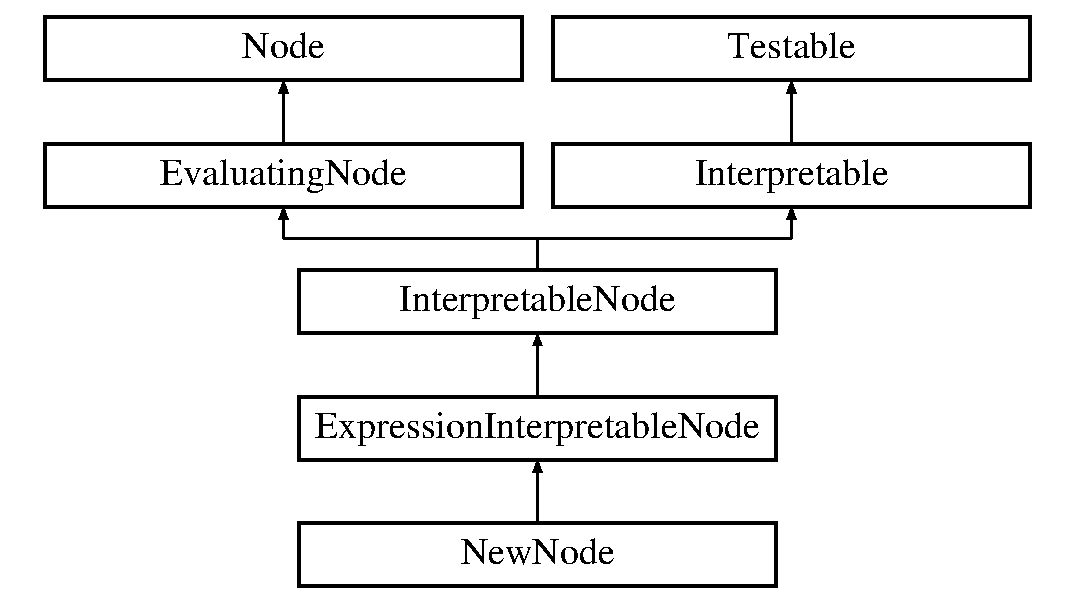
\includegraphics[height=5.000000cm]{classNewNode}
\end{center}
\end{figure}
\subsection*{Public Member Functions}
\begin{DoxyCompactItemize}
\item 
\hyperlink{classNewNode_a55edf2127f3cd875164a199029d7ebba}{New\+Node} ()
\item 
virtual \hyperlink{classNewNode_ab06c72bb48fc65bb12a21c1a6c3aa9c8}{$\sim$\+New\+Node} ()
\item 
bool \hyperlink{classNewNode_af2d1614a80b8fcc00957155109e4b2f2}{is\+Array} ()
\item 
virtual void \hyperlink{classNewNode_a9be504d069e8a5d4ea13b4767a3c792a}{test} (\hyperlink{classValidator}{Validator} $\ast$validator)
\item 
virtual \hyperlink{classValue}{Value} \hyperlink{classNewNode_a77447b9402f0153401bf0e623b5f1e6e}{interpret} (\hyperlink{classInterpreter}{Interpreter} $\ast$interpreter)
\item 
virtual void \hyperlink{classNewNode_a53fe843af3bbb2add900646ef3891f8e}{evaluate\+\_\+impl} (\hyperlink{classSystemHandler}{System\+Handler} $\ast$handler, \hyperlink{statics_8h_a6664c451ca7787483a7981cc1de68dbb}{E\+V\+A\+L\+U\+A\+T\+I\+O\+N\+\_\+\+T\+Y\+PE} expected\+\_\+evaluation, struct \hyperlink{structEvaluation}{Evaluation} $\ast$evaluation)
\end{DoxyCompactItemize}
\subsection*{Public Attributes}
\begin{DoxyCompactItemize}
\item 
\hyperlink{classExpressionInterpretableNode}{Expression\+Interpretable\+Node} $\ast$ \hyperlink{classNewNode_a1cf62395c1531a22ca8e1932ed82910c}{type\+\_\+node}
\item 
std\+::vector$<$ \hyperlink{classExpressionInterpretableNode}{Expression\+Interpretable\+Node} $\ast$ $>$ \hyperlink{classNewNode_afd78e7c3e05eb57a1536f705fb900fd5}{array\+\_\+values}
\end{DoxyCompactItemize}
\subsection*{Additional Inherited Members}


\subsection{Constructor \& Destructor Documentation}
\mbox{\Hypertarget{classNewNode_a55edf2127f3cd875164a199029d7ebba}\label{classNewNode_a55edf2127f3cd875164a199029d7ebba}} 
\index{New\+Node@{New\+Node}!New\+Node@{New\+Node}}
\index{New\+Node@{New\+Node}!New\+Node@{New\+Node}}
\subsubsection{\texorpdfstring{New\+Node()}{NewNode()}}
{\footnotesize\ttfamily New\+Node\+::\+New\+Node (\begin{DoxyParamCaption}{ }\end{DoxyParamCaption})}

\mbox{\Hypertarget{classNewNode_ab06c72bb48fc65bb12a21c1a6c3aa9c8}\label{classNewNode_ab06c72bb48fc65bb12a21c1a6c3aa9c8}} 
\index{New\+Node@{New\+Node}!````~New\+Node@{$\sim$\+New\+Node}}
\index{````~New\+Node@{$\sim$\+New\+Node}!New\+Node@{New\+Node}}
\subsubsection{\texorpdfstring{$\sim$\+New\+Node()}{~NewNode()}}
{\footnotesize\ttfamily virtual New\+Node\+::$\sim$\+New\+Node (\begin{DoxyParamCaption}{ }\end{DoxyParamCaption})\hspace{0.3cm}{\ttfamily [virtual]}}



\subsection{Member Function Documentation}
\mbox{\Hypertarget{classNewNode_a53fe843af3bbb2add900646ef3891f8e}\label{classNewNode_a53fe843af3bbb2add900646ef3891f8e}} 
\index{New\+Node@{New\+Node}!evaluate\+\_\+impl@{evaluate\+\_\+impl}}
\index{evaluate\+\_\+impl@{evaluate\+\_\+impl}!New\+Node@{New\+Node}}
\subsubsection{\texorpdfstring{evaluate\+\_\+impl()}{evaluate\_impl()}}
{\footnotesize\ttfamily virtual void New\+Node\+::evaluate\+\_\+impl (\begin{DoxyParamCaption}\item[{\hyperlink{classSystemHandler}{System\+Handler} $\ast$}]{handler,  }\item[{\hyperlink{statics_8h_a6664c451ca7787483a7981cc1de68dbb}{E\+V\+A\+L\+U\+A\+T\+I\+O\+N\+\_\+\+T\+Y\+PE}}]{expected\+\_\+evaluation,  }\item[{struct \hyperlink{structEvaluation}{Evaluation} $\ast$}]{evaluation }\end{DoxyParamCaption})\hspace{0.3cm}{\ttfamily [virtual]}}



Implements \hyperlink{classEvaluatingNode_a085fa06e0b46a93c814dc55cda0c1b26}{Evaluating\+Node}.

\mbox{\Hypertarget{classNewNode_a77447b9402f0153401bf0e623b5f1e6e}\label{classNewNode_a77447b9402f0153401bf0e623b5f1e6e}} 
\index{New\+Node@{New\+Node}!interpret@{interpret}}
\index{interpret@{interpret}!New\+Node@{New\+Node}}
\subsubsection{\texorpdfstring{interpret()}{interpret()}}
{\footnotesize\ttfamily virtual \hyperlink{classValue}{Value} New\+Node\+::interpret (\begin{DoxyParamCaption}\item[{\hyperlink{classInterpreter}{Interpreter} $\ast$}]{interpreter }\end{DoxyParamCaption})\hspace{0.3cm}{\ttfamily [virtual]}}



Implements \hyperlink{classExpressionInterpretableNode_a43650f046c48fc539f77a207e3c9181e}{Expression\+Interpretable\+Node}.

\mbox{\Hypertarget{classNewNode_af2d1614a80b8fcc00957155109e4b2f2}\label{classNewNode_af2d1614a80b8fcc00957155109e4b2f2}} 
\index{New\+Node@{New\+Node}!is\+Array@{is\+Array}}
\index{is\+Array@{is\+Array}!New\+Node@{New\+Node}}
\subsubsection{\texorpdfstring{is\+Array()}{isArray()}}
{\footnotesize\ttfamily bool New\+Node\+::is\+Array (\begin{DoxyParamCaption}{ }\end{DoxyParamCaption})}

\mbox{\Hypertarget{classNewNode_a9be504d069e8a5d4ea13b4767a3c792a}\label{classNewNode_a9be504d069e8a5d4ea13b4767a3c792a}} 
\index{New\+Node@{New\+Node}!test@{test}}
\index{test@{test}!New\+Node@{New\+Node}}
\subsubsection{\texorpdfstring{test()}{test()}}
{\footnotesize\ttfamily virtual void New\+Node\+::test (\begin{DoxyParamCaption}\item[{\hyperlink{classValidator}{Validator} $\ast$}]{validator }\end{DoxyParamCaption})\hspace{0.3cm}{\ttfamily [virtual]}}



Reimplemented from \hyperlink{classInterpretable_a32f547aaf68dcbab993284d3257ab010}{Interpretable}.



\subsection{Member Data Documentation}
\mbox{\Hypertarget{classNewNode_afd78e7c3e05eb57a1536f705fb900fd5}\label{classNewNode_afd78e7c3e05eb57a1536f705fb900fd5}} 
\index{New\+Node@{New\+Node}!array\+\_\+values@{array\+\_\+values}}
\index{array\+\_\+values@{array\+\_\+values}!New\+Node@{New\+Node}}
\subsubsection{\texorpdfstring{array\+\_\+values}{array\_values}}
{\footnotesize\ttfamily std\+::vector$<$\hyperlink{classExpressionInterpretableNode}{Expression\+Interpretable\+Node}$\ast$$>$ New\+Node\+::array\+\_\+values}

\mbox{\Hypertarget{classNewNode_a1cf62395c1531a22ca8e1932ed82910c}\label{classNewNode_a1cf62395c1531a22ca8e1932ed82910c}} 
\index{New\+Node@{New\+Node}!type\+\_\+node@{type\+\_\+node}}
\index{type\+\_\+node@{type\+\_\+node}!New\+Node@{New\+Node}}
\subsubsection{\texorpdfstring{type\+\_\+node}{type\_node}}
{\footnotesize\ttfamily \hyperlink{classExpressionInterpretableNode}{Expression\+Interpretable\+Node}$\ast$ New\+Node\+::type\+\_\+node}



The documentation for this class was generated from the following file\+:\begin{DoxyCompactItemize}
\item 
include/\hyperlink{newnode_8h}{newnode.\+h}\end{DoxyCompactItemize}

\hypertarget{classNode}{}\section{Node Class Reference}
\label{classNode}\index{Node@{Node}}


{\ttfamily \#include $<$node.\+h$>$}

Inheritance diagram for Node\+:\begin{figure}[H]
\begin{center}
\leavevmode
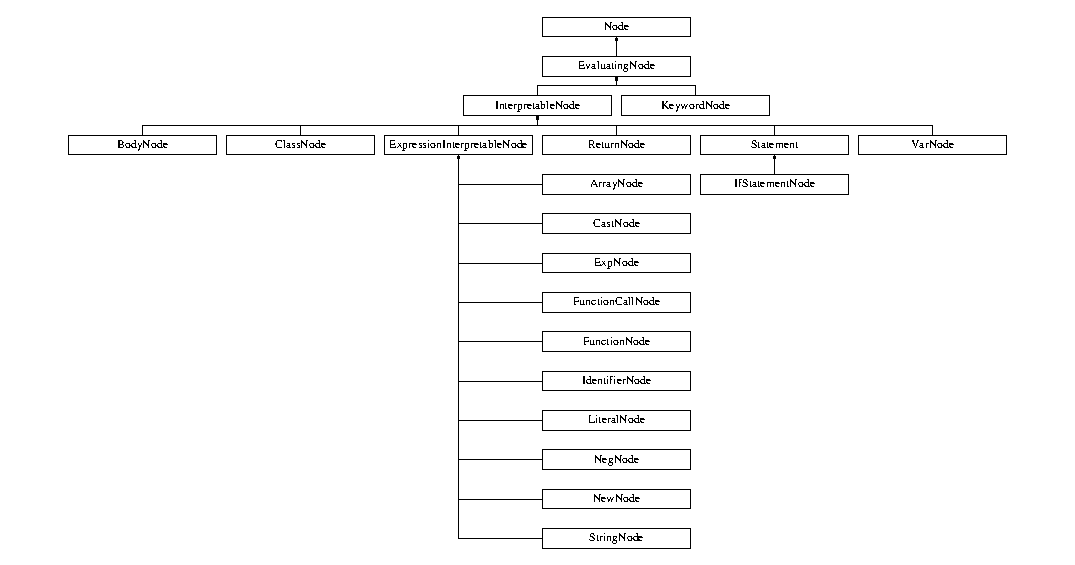
\includegraphics[height=7.140255cm]{classNode}
\end{center}
\end{figure}
\subsection*{Public Member Functions}
\begin{DoxyCompactItemize}
\item 
\hyperlink{classNode_a81891cf87be70506850d76a39dad29dd}{Node} (int \hyperlink{classNode_af4f536b1b3f60e197fe364ba56022291}{type})
\item 
virtual \hyperlink{classNode_af5e3fa79300bf5f3f2f3ecae6e795a94}{$\sim$\+Node} ()
\item 
int \hyperlink{classNode_a8de16678e4b507d5caee3fe52bfa053b}{get\+Type} ()
\end{DoxyCompactItemize}
\subsection*{Public Attributes}
\begin{DoxyCompactItemize}
\item 
\hyperlink{classNode}{Node} $\ast$ \hyperlink{classNode_a2559a716f69ccaa76d648d9f1b83065e}{next}
\item 
int const \hyperlink{classNode_af4f536b1b3f60e197fe364ba56022291}{type}
\item 
\hyperlink{classPosInfo}{Pos\+Info} \hyperlink{classNode_aa0e8a1e5aebdbe33183001b5a1c57111}{pos\+Info}
\end{DoxyCompactItemize}


\subsection{Constructor \& Destructor Documentation}
\mbox{\Hypertarget{classNode_a81891cf87be70506850d76a39dad29dd}\label{classNode_a81891cf87be70506850d76a39dad29dd}} 
\index{Node@{Node}!Node@{Node}}
\index{Node@{Node}!Node@{Node}}
\subsubsection{\texorpdfstring{Node()}{Node()}}
{\footnotesize\ttfamily Node\+::\+Node (\begin{DoxyParamCaption}\item[{int}]{type }\end{DoxyParamCaption})}

\mbox{\Hypertarget{classNode_af5e3fa79300bf5f3f2f3ecae6e795a94}\label{classNode_af5e3fa79300bf5f3f2f3ecae6e795a94}} 
\index{Node@{Node}!````~Node@{$\sim$\+Node}}
\index{````~Node@{$\sim$\+Node}!Node@{Node}}
\subsubsection{\texorpdfstring{$\sim$\+Node()}{~Node()}}
{\footnotesize\ttfamily virtual Node\+::$\sim$\+Node (\begin{DoxyParamCaption}{ }\end{DoxyParamCaption})\hspace{0.3cm}{\ttfamily [virtual]}}



\subsection{Member Function Documentation}
\mbox{\Hypertarget{classNode_a8de16678e4b507d5caee3fe52bfa053b}\label{classNode_a8de16678e4b507d5caee3fe52bfa053b}} 
\index{Node@{Node}!get\+Type@{get\+Type}}
\index{get\+Type@{get\+Type}!Node@{Node}}
\subsubsection{\texorpdfstring{get\+Type()}{getType()}}
{\footnotesize\ttfamily int Node\+::get\+Type (\begin{DoxyParamCaption}{ }\end{DoxyParamCaption})}



\subsection{Member Data Documentation}
\mbox{\Hypertarget{classNode_a2559a716f69ccaa76d648d9f1b83065e}\label{classNode_a2559a716f69ccaa76d648d9f1b83065e}} 
\index{Node@{Node}!next@{next}}
\index{next@{next}!Node@{Node}}
\subsubsection{\texorpdfstring{next}{next}}
{\footnotesize\ttfamily \hyperlink{classNode}{Node}$\ast$ Node\+::next}

\mbox{\Hypertarget{classNode_aa0e8a1e5aebdbe33183001b5a1c57111}\label{classNode_aa0e8a1e5aebdbe33183001b5a1c57111}} 
\index{Node@{Node}!pos\+Info@{pos\+Info}}
\index{pos\+Info@{pos\+Info}!Node@{Node}}
\subsubsection{\texorpdfstring{pos\+Info}{posInfo}}
{\footnotesize\ttfamily \hyperlink{classPosInfo}{Pos\+Info} Node\+::pos\+Info}

\mbox{\Hypertarget{classNode_af4f536b1b3f60e197fe364ba56022291}\label{classNode_af4f536b1b3f60e197fe364ba56022291}} 
\index{Node@{Node}!type@{type}}
\index{type@{type}!Node@{Node}}
\subsubsection{\texorpdfstring{type}{type}}
{\footnotesize\ttfamily int const Node\+::type}



The documentation for this class was generated from the following file\+:\begin{DoxyCompactItemize}
\item 
include/\hyperlink{node_8h}{node.\+h}\end{DoxyCompactItemize}

\hypertarget{classNodeFactory}{}\section{Node\+Factory Class Reference}
\label{classNodeFactory}\index{Node\+Factory@{Node\+Factory}}


{\ttfamily \#include $<$nodefactory.\+h$>$}

\subsection*{Public Member Functions}
\begin{DoxyCompactItemize}
\item 
\hyperlink{classNodeFactory_ac12b3627ac674658d29e4083a73b1e43}{Node\+Factory} ()
\item 
virtual \hyperlink{classNodeFactory_a1ce6fde33ca914e0b70f80ce2c730e37}{$\sim$\+Node\+Factory} ()
\item 
void \hyperlink{classNodeFactory_a9eb2e94e99b0c087968e76775fbbdf07}{apply\+Position} (\hyperlink{classPosInfo}{Pos\+Info} pos\+Info)
\item 
\hyperlink{classNode}{Node} $\ast$ \hyperlink{classNodeFactory_ac8757ee2441a4439b8bda6ed5296ede1}{create\+Node} (\hyperlink{statics_8h_a1ec6d4bfce2e004debbc141eafc512db}{N\+O\+D\+E\+\_\+\+T\+Y\+PE} node\+\_\+type)
\end{DoxyCompactItemize}


\subsection{Constructor \& Destructor Documentation}
\mbox{\Hypertarget{classNodeFactory_ac12b3627ac674658d29e4083a73b1e43}\label{classNodeFactory_ac12b3627ac674658d29e4083a73b1e43}} 
\index{Node\+Factory@{Node\+Factory}!Node\+Factory@{Node\+Factory}}
\index{Node\+Factory@{Node\+Factory}!Node\+Factory@{Node\+Factory}}
\subsubsection{\texorpdfstring{Node\+Factory()}{NodeFactory()}}
{\footnotesize\ttfamily Node\+Factory\+::\+Node\+Factory (\begin{DoxyParamCaption}{ }\end{DoxyParamCaption})}

\mbox{\Hypertarget{classNodeFactory_a1ce6fde33ca914e0b70f80ce2c730e37}\label{classNodeFactory_a1ce6fde33ca914e0b70f80ce2c730e37}} 
\index{Node\+Factory@{Node\+Factory}!````~Node\+Factory@{$\sim$\+Node\+Factory}}
\index{````~Node\+Factory@{$\sim$\+Node\+Factory}!Node\+Factory@{Node\+Factory}}
\subsubsection{\texorpdfstring{$\sim$\+Node\+Factory()}{~NodeFactory()}}
{\footnotesize\ttfamily virtual Node\+Factory\+::$\sim$\+Node\+Factory (\begin{DoxyParamCaption}{ }\end{DoxyParamCaption})\hspace{0.3cm}{\ttfamily [virtual]}}



\subsection{Member Function Documentation}
\mbox{\Hypertarget{classNodeFactory_a9eb2e94e99b0c087968e76775fbbdf07}\label{classNodeFactory_a9eb2e94e99b0c087968e76775fbbdf07}} 
\index{Node\+Factory@{Node\+Factory}!apply\+Position@{apply\+Position}}
\index{apply\+Position@{apply\+Position}!Node\+Factory@{Node\+Factory}}
\subsubsection{\texorpdfstring{apply\+Position()}{applyPosition()}}
{\footnotesize\ttfamily void Node\+Factory\+::apply\+Position (\begin{DoxyParamCaption}\item[{\hyperlink{classPosInfo}{Pos\+Info}}]{pos\+Info }\end{DoxyParamCaption})}

\mbox{\Hypertarget{classNodeFactory_ac8757ee2441a4439b8bda6ed5296ede1}\label{classNodeFactory_ac8757ee2441a4439b8bda6ed5296ede1}} 
\index{Node\+Factory@{Node\+Factory}!create\+Node@{create\+Node}}
\index{create\+Node@{create\+Node}!Node\+Factory@{Node\+Factory}}
\subsubsection{\texorpdfstring{create\+Node()}{createNode()}}
{\footnotesize\ttfamily \hyperlink{classNode}{Node}$\ast$ Node\+Factory\+::create\+Node (\begin{DoxyParamCaption}\item[{\hyperlink{statics_8h_a1ec6d4bfce2e004debbc141eafc512db}{N\+O\+D\+E\+\_\+\+T\+Y\+PE}}]{node\+\_\+type }\end{DoxyParamCaption})}



The documentation for this class was generated from the following file\+:\begin{DoxyCompactItemize}
\item 
include/\hyperlink{nodefactory_8h}{nodefactory.\+h}\end{DoxyCompactItemize}

\hypertarget{classObject}{}\section{Object Class Reference}
\label{classObject}\index{Object@{Object}}


{\ttfamily \#include $<$object.\+h$>$}

Inheritance diagram for Object\+:\begin{figure}[H]
\begin{center}
\leavevmode
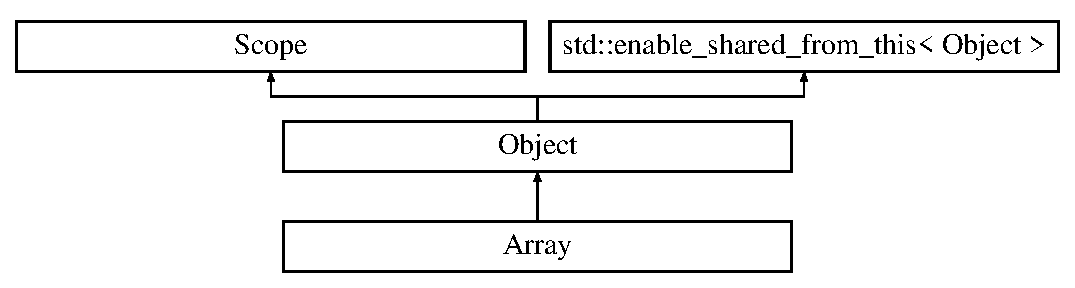
\includegraphics[height=3.000000cm]{classObject}
\end{center}
\end{figure}
\subsection*{Public Member Functions}
\begin{DoxyCompactItemize}
\item 
\hyperlink{classObject_a208aa5ccaeae34404f1ebacdfec66fbb}{Object} (\hyperlink{classSystemHandler}{System\+Handler} $\ast$sys\+\_\+handler, \hyperlink{classClass}{Class} $\ast$c)
\item 
virtual \hyperlink{classObject_aa3e791419d84c4c346ef9499513b8e00}{$\sim$\+Object} ()
\item 
virtual void \hyperlink{classObject_ad8f3631de109f50f94432ae9e1f7a130}{register\+Variable} (\hyperlink{classVariable}{Variable} $\ast$variable)
\item 
\hyperlink{classClass}{Class} $\ast$ \hyperlink{classObject_a51f229ad629a4ac1ad6e359a3b53941d}{get\+Class} ()
\item 
virtual void \hyperlink{classObject_a61b4cd86dd434abf07e3f4d19b5c93eb}{on\+Enter\+Scope} ()
\item 
virtual void \hyperlink{classObject_a54a99563b5936626d47fb1e2f0e13a9c}{on\+Leave\+Scope} ()
\end{DoxyCompactItemize}
\subsection*{Additional Inherited Members}


\subsection{Constructor \& Destructor Documentation}
\mbox{\Hypertarget{classObject_a208aa5ccaeae34404f1ebacdfec66fbb}\label{classObject_a208aa5ccaeae34404f1ebacdfec66fbb}} 
\index{Object@{Object}!Object@{Object}}
\index{Object@{Object}!Object@{Object}}
\subsubsection{\texorpdfstring{Object()}{Object()}}
{\footnotesize\ttfamily Object\+::\+Object (\begin{DoxyParamCaption}\item[{\hyperlink{classSystemHandler}{System\+Handler} $\ast$}]{sys\+\_\+handler,  }\item[{\hyperlink{classClass}{Class} $\ast$}]{c }\end{DoxyParamCaption})}

\mbox{\Hypertarget{classObject_aa3e791419d84c4c346ef9499513b8e00}\label{classObject_aa3e791419d84c4c346ef9499513b8e00}} 
\index{Object@{Object}!````~Object@{$\sim$\+Object}}
\index{````~Object@{$\sim$\+Object}!Object@{Object}}
\subsubsection{\texorpdfstring{$\sim$\+Object()}{~Object()}}
{\footnotesize\ttfamily virtual Object\+::$\sim$\+Object (\begin{DoxyParamCaption}{ }\end{DoxyParamCaption})\hspace{0.3cm}{\ttfamily [virtual]}}



\subsection{Member Function Documentation}
\mbox{\Hypertarget{classObject_a51f229ad629a4ac1ad6e359a3b53941d}\label{classObject_a51f229ad629a4ac1ad6e359a3b53941d}} 
\index{Object@{Object}!get\+Class@{get\+Class}}
\index{get\+Class@{get\+Class}!Object@{Object}}
\subsubsection{\texorpdfstring{get\+Class()}{getClass()}}
{\footnotesize\ttfamily \hyperlink{classClass}{Class}$\ast$ Object\+::get\+Class (\begin{DoxyParamCaption}{ }\end{DoxyParamCaption})}

\mbox{\Hypertarget{classObject_a61b4cd86dd434abf07e3f4d19b5c93eb}\label{classObject_a61b4cd86dd434abf07e3f4d19b5c93eb}} 
\index{Object@{Object}!on\+Enter\+Scope@{on\+Enter\+Scope}}
\index{on\+Enter\+Scope@{on\+Enter\+Scope}!Object@{Object}}
\subsubsection{\texorpdfstring{on\+Enter\+Scope()}{onEnterScope()}}
{\footnotesize\ttfamily virtual void Object\+::on\+Enter\+Scope (\begin{DoxyParamCaption}{ }\end{DoxyParamCaption})\hspace{0.3cm}{\ttfamily [virtual]}}



Reimplemented from \hyperlink{classScope_a4a42aaa7bd341ef07a90ef51860f0a8a}{Scope}.

\mbox{\Hypertarget{classObject_a54a99563b5936626d47fb1e2f0e13a9c}\label{classObject_a54a99563b5936626d47fb1e2f0e13a9c}} 
\index{Object@{Object}!on\+Leave\+Scope@{on\+Leave\+Scope}}
\index{on\+Leave\+Scope@{on\+Leave\+Scope}!Object@{Object}}
\subsubsection{\texorpdfstring{on\+Leave\+Scope()}{onLeaveScope()}}
{\footnotesize\ttfamily virtual void Object\+::on\+Leave\+Scope (\begin{DoxyParamCaption}{ }\end{DoxyParamCaption})\hspace{0.3cm}{\ttfamily [virtual]}}



Reimplemented from \hyperlink{classScope_acff92230877eb8ff60f27c86ac56e929}{Scope}.

\mbox{\Hypertarget{classObject_ad8f3631de109f50f94432ae9e1f7a130}\label{classObject_ad8f3631de109f50f94432ae9e1f7a130}} 
\index{Object@{Object}!register\+Variable@{register\+Variable}}
\index{register\+Variable@{register\+Variable}!Object@{Object}}
\subsubsection{\texorpdfstring{register\+Variable()}{registerVariable()}}
{\footnotesize\ttfamily virtual void Object\+::register\+Variable (\begin{DoxyParamCaption}\item[{\hyperlink{classVariable}{Variable} $\ast$}]{variable }\end{DoxyParamCaption})\hspace{0.3cm}{\ttfamily [virtual]}}



Reimplemented from \hyperlink{classScope_a4c2622adf1835753f5233869febd80d4}{Scope}.



The documentation for this class was generated from the following file\+:\begin{DoxyCompactItemize}
\item 
include/\hyperlink{object_8h}{object.\+h}\end{DoxyCompactItemize}

\hypertarget{structorder__of__operation}{}\section{order\+\_\+of\+\_\+operation Struct Reference}
\label{structorder__of__operation}\index{order\+\_\+of\+\_\+operation@{order\+\_\+of\+\_\+operation}}


{\ttfamily \#include $<$parser.\+h$>$}

\subsection*{Public Attributes}
\begin{DoxyCompactItemize}
\item 
const char $\ast$ \hyperlink{structorder__of__operation_a841a4b6a7e32e889adabd89b818823d7}{op}
\item 
int \hyperlink{structorder__of__operation_a473d1dd1e8d79cfa6c2e84bb7402da14}{priority}
\item 
int \hyperlink{structorder__of__operation_ac799b9d51e112ea751f8f264a8962591}{associativity}
\end{DoxyCompactItemize}


\subsection{Member Data Documentation}
\mbox{\Hypertarget{structorder__of__operation_ac799b9d51e112ea751f8f264a8962591}\label{structorder__of__operation_ac799b9d51e112ea751f8f264a8962591}} 
\index{order\+\_\+of\+\_\+operation@{order\+\_\+of\+\_\+operation}!associativity@{associativity}}
\index{associativity@{associativity}!order\+\_\+of\+\_\+operation@{order\+\_\+of\+\_\+operation}}
\subsubsection{\texorpdfstring{associativity}{associativity}}
{\footnotesize\ttfamily int order\+\_\+of\+\_\+operation\+::associativity}

\mbox{\Hypertarget{structorder__of__operation_a841a4b6a7e32e889adabd89b818823d7}\label{structorder__of__operation_a841a4b6a7e32e889adabd89b818823d7}} 
\index{order\+\_\+of\+\_\+operation@{order\+\_\+of\+\_\+operation}!op@{op}}
\index{op@{op}!order\+\_\+of\+\_\+operation@{order\+\_\+of\+\_\+operation}}
\subsubsection{\texorpdfstring{op}{op}}
{\footnotesize\ttfamily const char$\ast$ order\+\_\+of\+\_\+operation\+::op}

\mbox{\Hypertarget{structorder__of__operation_a473d1dd1e8d79cfa6c2e84bb7402da14}\label{structorder__of__operation_a473d1dd1e8d79cfa6c2e84bb7402da14}} 
\index{order\+\_\+of\+\_\+operation@{order\+\_\+of\+\_\+operation}!priority@{priority}}
\index{priority@{priority}!order\+\_\+of\+\_\+operation@{order\+\_\+of\+\_\+operation}}
\subsubsection{\texorpdfstring{priority}{priority}}
{\footnotesize\ttfamily int order\+\_\+of\+\_\+operation\+::priority}



The documentation for this struct was generated from the following file\+:\begin{DoxyCompactItemize}
\item 
include/\hyperlink{parser_8h}{parser.\+h}\end{DoxyCompactItemize}

\hypertarget{structoutput__data}{}\section{output\+\_\+data Struct Reference}
\label{structoutput__data}\index{output\+\_\+data@{output\+\_\+data}}


{\ttfamily \#include $<$splitter.\+h$>$}

Inheritance diagram for output\+\_\+data\+:\begin{figure}[H]
\begin{center}
\leavevmode
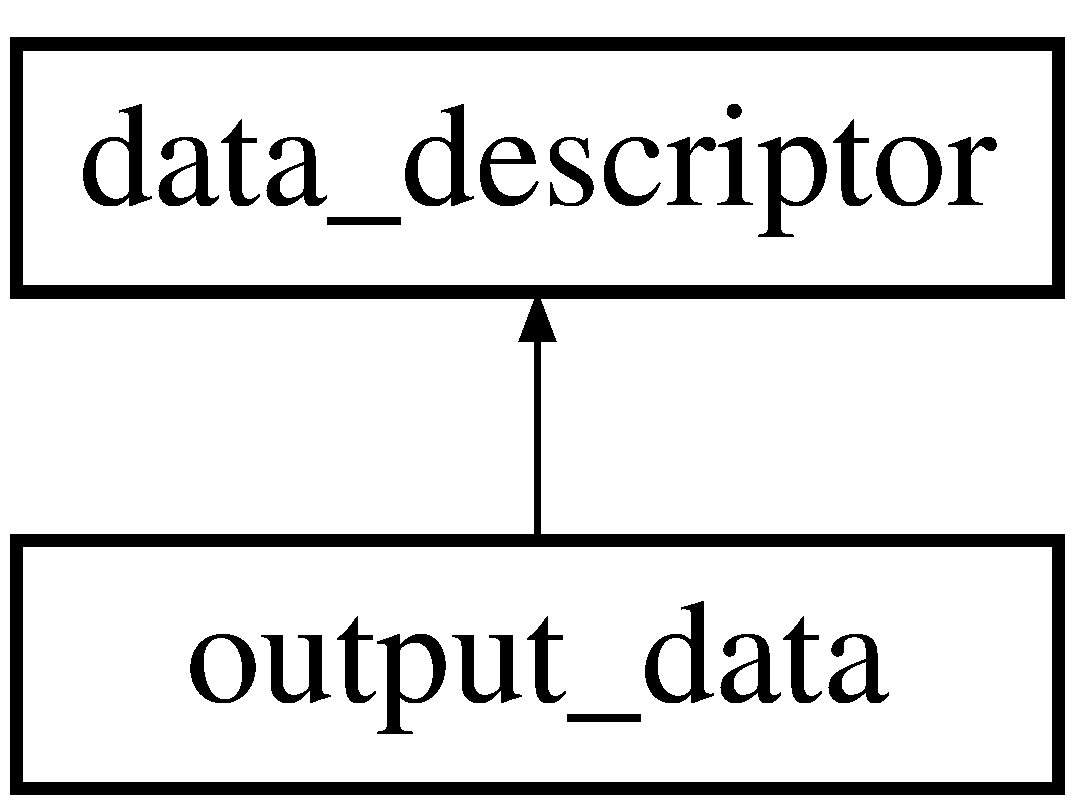
\includegraphics[height=2.000000cm]{structoutput__data}
\end{center}
\end{figure}
\subsection*{Public Member Functions}
\begin{DoxyCompactItemize}
\item 
void \hyperlink{structoutput__data_ad3dd0b4e74cd55dee641af403690ed64}{update} ()
\end{DoxyCompactItemize}
\subsection*{Additional Inherited Members}


\subsection{Member Function Documentation}
\mbox{\Hypertarget{structoutput__data_ad3dd0b4e74cd55dee641af403690ed64}\label{structoutput__data_ad3dd0b4e74cd55dee641af403690ed64}} 
\index{output\+\_\+data@{output\+\_\+data}!update@{update}}
\index{update@{update}!output\+\_\+data@{output\+\_\+data}}
\subsubsection{\texorpdfstring{update()}{update()}}
{\footnotesize\ttfamily void output\+\_\+data\+::update (\begin{DoxyParamCaption}{ }\end{DoxyParamCaption})\hspace{0.3cm}{\ttfamily [virtual]}}



Reimplemented from \hyperlink{structdata__descriptor_ad6cd92beb7d2b9291e0d130a24faa380}{data\+\_\+descriptor}.



The documentation for this struct was generated from the following file\+:\begin{DoxyCompactItemize}
\item 
include/\hyperlink{splitter_8h}{splitter.\+h}\end{DoxyCompactItemize}

\hypertarget{classParser}{}\section{Parser Class Reference}
\label{classParser}\index{Parser@{Parser}}


{\ttfamily \#include $<$parser.\+h$>$}

\subsection*{Public Member Functions}
\begin{DoxyCompactItemize}
\item 
\hyperlink{classParser_a803d4bd64cf277f60b98e52d3dbc7220}{Parser} (\hyperlink{classLogger}{Logger} $\ast$logger)
\item 
virtual \hyperlink{classParser_ad576b92b9cc324f6f41b0269a9a1a546}{$\sim$\+Parser} ()
\item 
\hyperlink{classNode}{Node} $\ast$ \hyperlink{classParser_ab6d7f459c011482f94ee185fc4779168}{parse} (\hyperlink{classToken}{Token} $\ast$root\+\_\+token)
\item 
\hyperlink{classLogger}{Logger} $\ast$ \hyperlink{classParser_a87f0d3ea4178cfba8aaf9f898ce899e6}{get\+Logger} ()
\end{DoxyCompactItemize}


\subsection{Constructor \& Destructor Documentation}
\mbox{\Hypertarget{classParser_a803d4bd64cf277f60b98e52d3dbc7220}\label{classParser_a803d4bd64cf277f60b98e52d3dbc7220}} 
\index{Parser@{Parser}!Parser@{Parser}}
\index{Parser@{Parser}!Parser@{Parser}}
\subsubsection{\texorpdfstring{Parser()}{Parser()}}
{\footnotesize\ttfamily Parser\+::\+Parser (\begin{DoxyParamCaption}\item[{\hyperlink{classLogger}{Logger} $\ast$}]{logger }\end{DoxyParamCaption})}

\mbox{\Hypertarget{classParser_ad576b92b9cc324f6f41b0269a9a1a546}\label{classParser_ad576b92b9cc324f6f41b0269a9a1a546}} 
\index{Parser@{Parser}!````~Parser@{$\sim$\+Parser}}
\index{````~Parser@{$\sim$\+Parser}!Parser@{Parser}}
\subsubsection{\texorpdfstring{$\sim$\+Parser()}{~Parser()}}
{\footnotesize\ttfamily virtual Parser\+::$\sim$\+Parser (\begin{DoxyParamCaption}{ }\end{DoxyParamCaption})\hspace{0.3cm}{\ttfamily [virtual]}}



\subsection{Member Function Documentation}
\mbox{\Hypertarget{classParser_a87f0d3ea4178cfba8aaf9f898ce899e6}\label{classParser_a87f0d3ea4178cfba8aaf9f898ce899e6}} 
\index{Parser@{Parser}!get\+Logger@{get\+Logger}}
\index{get\+Logger@{get\+Logger}!Parser@{Parser}}
\subsubsection{\texorpdfstring{get\+Logger()}{getLogger()}}
{\footnotesize\ttfamily \hyperlink{classLogger}{Logger}$\ast$ Parser\+::get\+Logger (\begin{DoxyParamCaption}{ }\end{DoxyParamCaption})}

\mbox{\Hypertarget{classParser_ab6d7f459c011482f94ee185fc4779168}\label{classParser_ab6d7f459c011482f94ee185fc4779168}} 
\index{Parser@{Parser}!parse@{parse}}
\index{parse@{parse}!Parser@{Parser}}
\subsubsection{\texorpdfstring{parse()}{parse()}}
{\footnotesize\ttfamily \hyperlink{classNode}{Node}$\ast$ Parser\+::parse (\begin{DoxyParamCaption}\item[{\hyperlink{classToken}{Token} $\ast$}]{root\+\_\+token }\end{DoxyParamCaption})}



The documentation for this class was generated from the following file\+:\begin{DoxyCompactItemize}
\item 
include/\hyperlink{parser_8h}{parser.\+h}\end{DoxyCompactItemize}

\hypertarget{classPosInfo}{}\section{Pos\+Info Class Reference}
\label{classPosInfo}\index{Pos\+Info@{Pos\+Info}}


{\ttfamily \#include $<$posinfo.\+h$>$}

\subsection*{Public Member Functions}
\begin{DoxyCompactItemize}
\item 
\hyperlink{classPosInfo_a828283f9428c078fa1c7df2ef3f48e2d}{Pos\+Info} ()
\item 
\hyperlink{classPosInfo_a87acb37bde91b4da7fadeaba819d16d8}{Pos\+Info} (int \hyperlink{classPosInfo_a1fbd2d0d0f4d2a20ade06f08e992da2c}{line}, int \hyperlink{classPosInfo_a7507047c71abe1f3db13b41ee340cc59}{col}, const char $\ast$\hyperlink{classPosInfo_acba31490cee179567ed7ab6a4c0c861b}{filename})
\item 
virtual \hyperlink{classPosInfo_a81518b89d4191e84f9de8f9c2d527577}{$\sim$\+Pos\+Info} ()
\end{DoxyCompactItemize}
\subsection*{Public Attributes}
\begin{DoxyCompactItemize}
\item 
int \hyperlink{classPosInfo_a1fbd2d0d0f4d2a20ade06f08e992da2c}{line}
\item 
int \hyperlink{classPosInfo_a7507047c71abe1f3db13b41ee340cc59}{col}
\item 
const char $\ast$ \hyperlink{classPosInfo_acba31490cee179567ed7ab6a4c0c861b}{filename}
\end{DoxyCompactItemize}


\subsection{Constructor \& Destructor Documentation}
\mbox{\Hypertarget{classPosInfo_a828283f9428c078fa1c7df2ef3f48e2d}\label{classPosInfo_a828283f9428c078fa1c7df2ef3f48e2d}} 
\index{Pos\+Info@{Pos\+Info}!Pos\+Info@{Pos\+Info}}
\index{Pos\+Info@{Pos\+Info}!Pos\+Info@{Pos\+Info}}
\subsubsection{\texorpdfstring{Pos\+Info()}{PosInfo()}\hspace{0.1cm}{\footnotesize\ttfamily [1/2]}}
{\footnotesize\ttfamily Pos\+Info\+::\+Pos\+Info (\begin{DoxyParamCaption}{ }\end{DoxyParamCaption})}

\mbox{\Hypertarget{classPosInfo_a87acb37bde91b4da7fadeaba819d16d8}\label{classPosInfo_a87acb37bde91b4da7fadeaba819d16d8}} 
\index{Pos\+Info@{Pos\+Info}!Pos\+Info@{Pos\+Info}}
\index{Pos\+Info@{Pos\+Info}!Pos\+Info@{Pos\+Info}}
\subsubsection{\texorpdfstring{Pos\+Info()}{PosInfo()}\hspace{0.1cm}{\footnotesize\ttfamily [2/2]}}
{\footnotesize\ttfamily Pos\+Info\+::\+Pos\+Info (\begin{DoxyParamCaption}\item[{int}]{line,  }\item[{int}]{col,  }\item[{const char $\ast$}]{filename }\end{DoxyParamCaption})}

\mbox{\Hypertarget{classPosInfo_a81518b89d4191e84f9de8f9c2d527577}\label{classPosInfo_a81518b89d4191e84f9de8f9c2d527577}} 
\index{Pos\+Info@{Pos\+Info}!````~Pos\+Info@{$\sim$\+Pos\+Info}}
\index{````~Pos\+Info@{$\sim$\+Pos\+Info}!Pos\+Info@{Pos\+Info}}
\subsubsection{\texorpdfstring{$\sim$\+Pos\+Info()}{~PosInfo()}}
{\footnotesize\ttfamily virtual Pos\+Info\+::$\sim$\+Pos\+Info (\begin{DoxyParamCaption}{ }\end{DoxyParamCaption})\hspace{0.3cm}{\ttfamily [virtual]}}



\subsection{Member Data Documentation}
\mbox{\Hypertarget{classPosInfo_a7507047c71abe1f3db13b41ee340cc59}\label{classPosInfo_a7507047c71abe1f3db13b41ee340cc59}} 
\index{Pos\+Info@{Pos\+Info}!col@{col}}
\index{col@{col}!Pos\+Info@{Pos\+Info}}
\subsubsection{\texorpdfstring{col}{col}}
{\footnotesize\ttfamily int Pos\+Info\+::col}

\mbox{\Hypertarget{classPosInfo_acba31490cee179567ed7ab6a4c0c861b}\label{classPosInfo_acba31490cee179567ed7ab6a4c0c861b}} 
\index{Pos\+Info@{Pos\+Info}!filename@{filename}}
\index{filename@{filename}!Pos\+Info@{Pos\+Info}}
\subsubsection{\texorpdfstring{filename}{filename}}
{\footnotesize\ttfamily const char$\ast$ Pos\+Info\+::filename}

\mbox{\Hypertarget{classPosInfo_a1fbd2d0d0f4d2a20ade06f08e992da2c}\label{classPosInfo_a1fbd2d0d0f4d2a20ade06f08e992da2c}} 
\index{Pos\+Info@{Pos\+Info}!line@{line}}
\index{line@{line}!Pos\+Info@{Pos\+Info}}
\subsubsection{\texorpdfstring{line}{line}}
{\footnotesize\ttfamily int Pos\+Info\+::line}



The documentation for this class was generated from the following file\+:\begin{DoxyCompactItemize}
\item 
include/\hyperlink{posinfo_8h}{posinfo.\+h}\end{DoxyCompactItemize}

\hypertarget{classReturnNode}{}\section{Return\+Node Class Reference}
\label{classReturnNode}\index{Return\+Node@{Return\+Node}}


{\ttfamily \#include $<$retnode.\+h$>$}

Inheritance diagram for Return\+Node\+:\begin{figure}[H]
\begin{center}
\leavevmode
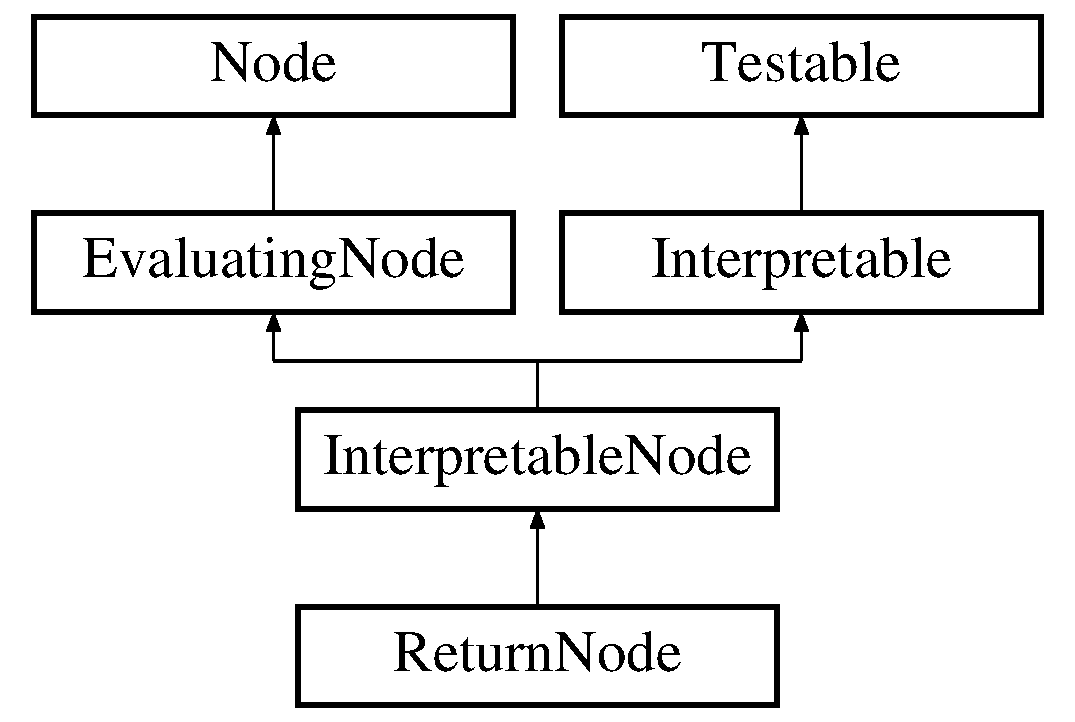
\includegraphics[height=4.000000cm]{classReturnNode}
\end{center}
\end{figure}
\subsection*{Public Member Functions}
\begin{DoxyCompactItemize}
\item 
\hyperlink{classReturnNode_a1e79c04a4e82c37af4aafa39be12b3ba}{Return\+Node} ()
\item 
virtual \hyperlink{classReturnNode_ab6ad8adf03f6c24bf9d717c6f1af7bcb}{$\sim$\+Return\+Node} ()
\item 
virtual \hyperlink{classValue}{Value} \hyperlink{classReturnNode_ae6c35829787a4f880b3ee1fa4b2e98d3}{interpret} (\hyperlink{classInterpreter}{Interpreter} $\ast$interpreter)
\item 
virtual void \hyperlink{classReturnNode_ac07545808632b52ec192cce2dd80b051}{evaluate\+\_\+impl} (\hyperlink{classSystemHandler}{System\+Handler} $\ast$handler, \hyperlink{statics_8h_a6664c451ca7787483a7981cc1de68dbb}{E\+V\+A\+L\+U\+A\+T\+I\+O\+N\+\_\+\+T\+Y\+PE} expected\+\_\+evaluation, struct \hyperlink{structEvaluation}{Evaluation} $\ast$evaluation)
\end{DoxyCompactItemize}
\subsection*{Public Attributes}
\begin{DoxyCompactItemize}
\item 
\hyperlink{classExpressionInterpretableNode}{Expression\+Interpretable\+Node} $\ast$ \hyperlink{classReturnNode_a27f21d586d90935184261ea34cf2a253}{exp}
\end{DoxyCompactItemize}
\subsection*{Additional Inherited Members}


\subsection{Constructor \& Destructor Documentation}
\mbox{\Hypertarget{classReturnNode_a1e79c04a4e82c37af4aafa39be12b3ba}\label{classReturnNode_a1e79c04a4e82c37af4aafa39be12b3ba}} 
\index{Return\+Node@{Return\+Node}!Return\+Node@{Return\+Node}}
\index{Return\+Node@{Return\+Node}!Return\+Node@{Return\+Node}}
\subsubsection{\texorpdfstring{Return\+Node()}{ReturnNode()}}
{\footnotesize\ttfamily Return\+Node\+::\+Return\+Node (\begin{DoxyParamCaption}{ }\end{DoxyParamCaption})}

\mbox{\Hypertarget{classReturnNode_ab6ad8adf03f6c24bf9d717c6f1af7bcb}\label{classReturnNode_ab6ad8adf03f6c24bf9d717c6f1af7bcb}} 
\index{Return\+Node@{Return\+Node}!````~Return\+Node@{$\sim$\+Return\+Node}}
\index{````~Return\+Node@{$\sim$\+Return\+Node}!Return\+Node@{Return\+Node}}
\subsubsection{\texorpdfstring{$\sim$\+Return\+Node()}{~ReturnNode()}}
{\footnotesize\ttfamily virtual Return\+Node\+::$\sim$\+Return\+Node (\begin{DoxyParamCaption}{ }\end{DoxyParamCaption})\hspace{0.3cm}{\ttfamily [virtual]}}



\subsection{Member Function Documentation}
\mbox{\Hypertarget{classReturnNode_ac07545808632b52ec192cce2dd80b051}\label{classReturnNode_ac07545808632b52ec192cce2dd80b051}} 
\index{Return\+Node@{Return\+Node}!evaluate\+\_\+impl@{evaluate\+\_\+impl}}
\index{evaluate\+\_\+impl@{evaluate\+\_\+impl}!Return\+Node@{Return\+Node}}
\subsubsection{\texorpdfstring{evaluate\+\_\+impl()}{evaluate\_impl()}}
{\footnotesize\ttfamily virtual void Return\+Node\+::evaluate\+\_\+impl (\begin{DoxyParamCaption}\item[{\hyperlink{classSystemHandler}{System\+Handler} $\ast$}]{handler,  }\item[{\hyperlink{statics_8h_a6664c451ca7787483a7981cc1de68dbb}{E\+V\+A\+L\+U\+A\+T\+I\+O\+N\+\_\+\+T\+Y\+PE}}]{expected\+\_\+evaluation,  }\item[{struct \hyperlink{structEvaluation}{Evaluation} $\ast$}]{evaluation }\end{DoxyParamCaption})\hspace{0.3cm}{\ttfamily [virtual]}}



Implements \hyperlink{classEvaluatingNode_a085fa06e0b46a93c814dc55cda0c1b26}{Evaluating\+Node}.

\mbox{\Hypertarget{classReturnNode_ae6c35829787a4f880b3ee1fa4b2e98d3}\label{classReturnNode_ae6c35829787a4f880b3ee1fa4b2e98d3}} 
\index{Return\+Node@{Return\+Node}!interpret@{interpret}}
\index{interpret@{interpret}!Return\+Node@{Return\+Node}}
\subsubsection{\texorpdfstring{interpret()}{interpret()}}
{\footnotesize\ttfamily virtual \hyperlink{classValue}{Value} Return\+Node\+::interpret (\begin{DoxyParamCaption}\item[{\hyperlink{classInterpreter}{Interpreter} $\ast$}]{interpreter }\end{DoxyParamCaption})\hspace{0.3cm}{\ttfamily [virtual]}}



Implements \hyperlink{classInterpretableNode_a9a466e7d65c4b323d2b96b4ac8396cd7}{Interpretable\+Node}.



\subsection{Member Data Documentation}
\mbox{\Hypertarget{classReturnNode_a27f21d586d90935184261ea34cf2a253}\label{classReturnNode_a27f21d586d90935184261ea34cf2a253}} 
\index{Return\+Node@{Return\+Node}!exp@{exp}}
\index{exp@{exp}!Return\+Node@{Return\+Node}}
\subsubsection{\texorpdfstring{exp}{exp}}
{\footnotesize\ttfamily \hyperlink{classExpressionInterpretableNode}{Expression\+Interpretable\+Node}$\ast$ Return\+Node\+::exp}



The documentation for this class was generated from the following file\+:\begin{DoxyCompactItemize}
\item 
include/\hyperlink{retnode_8h}{retnode.\+h}\end{DoxyCompactItemize}

\hypertarget{classScope}{}\section{Scope Class Reference}
\label{classScope}\index{Scope@{Scope}}


{\ttfamily \#include $<$scope.\+h$>$}

Inheritance diagram for Scope\+:\begin{figure}[H]
\begin{center}
\leavevmode
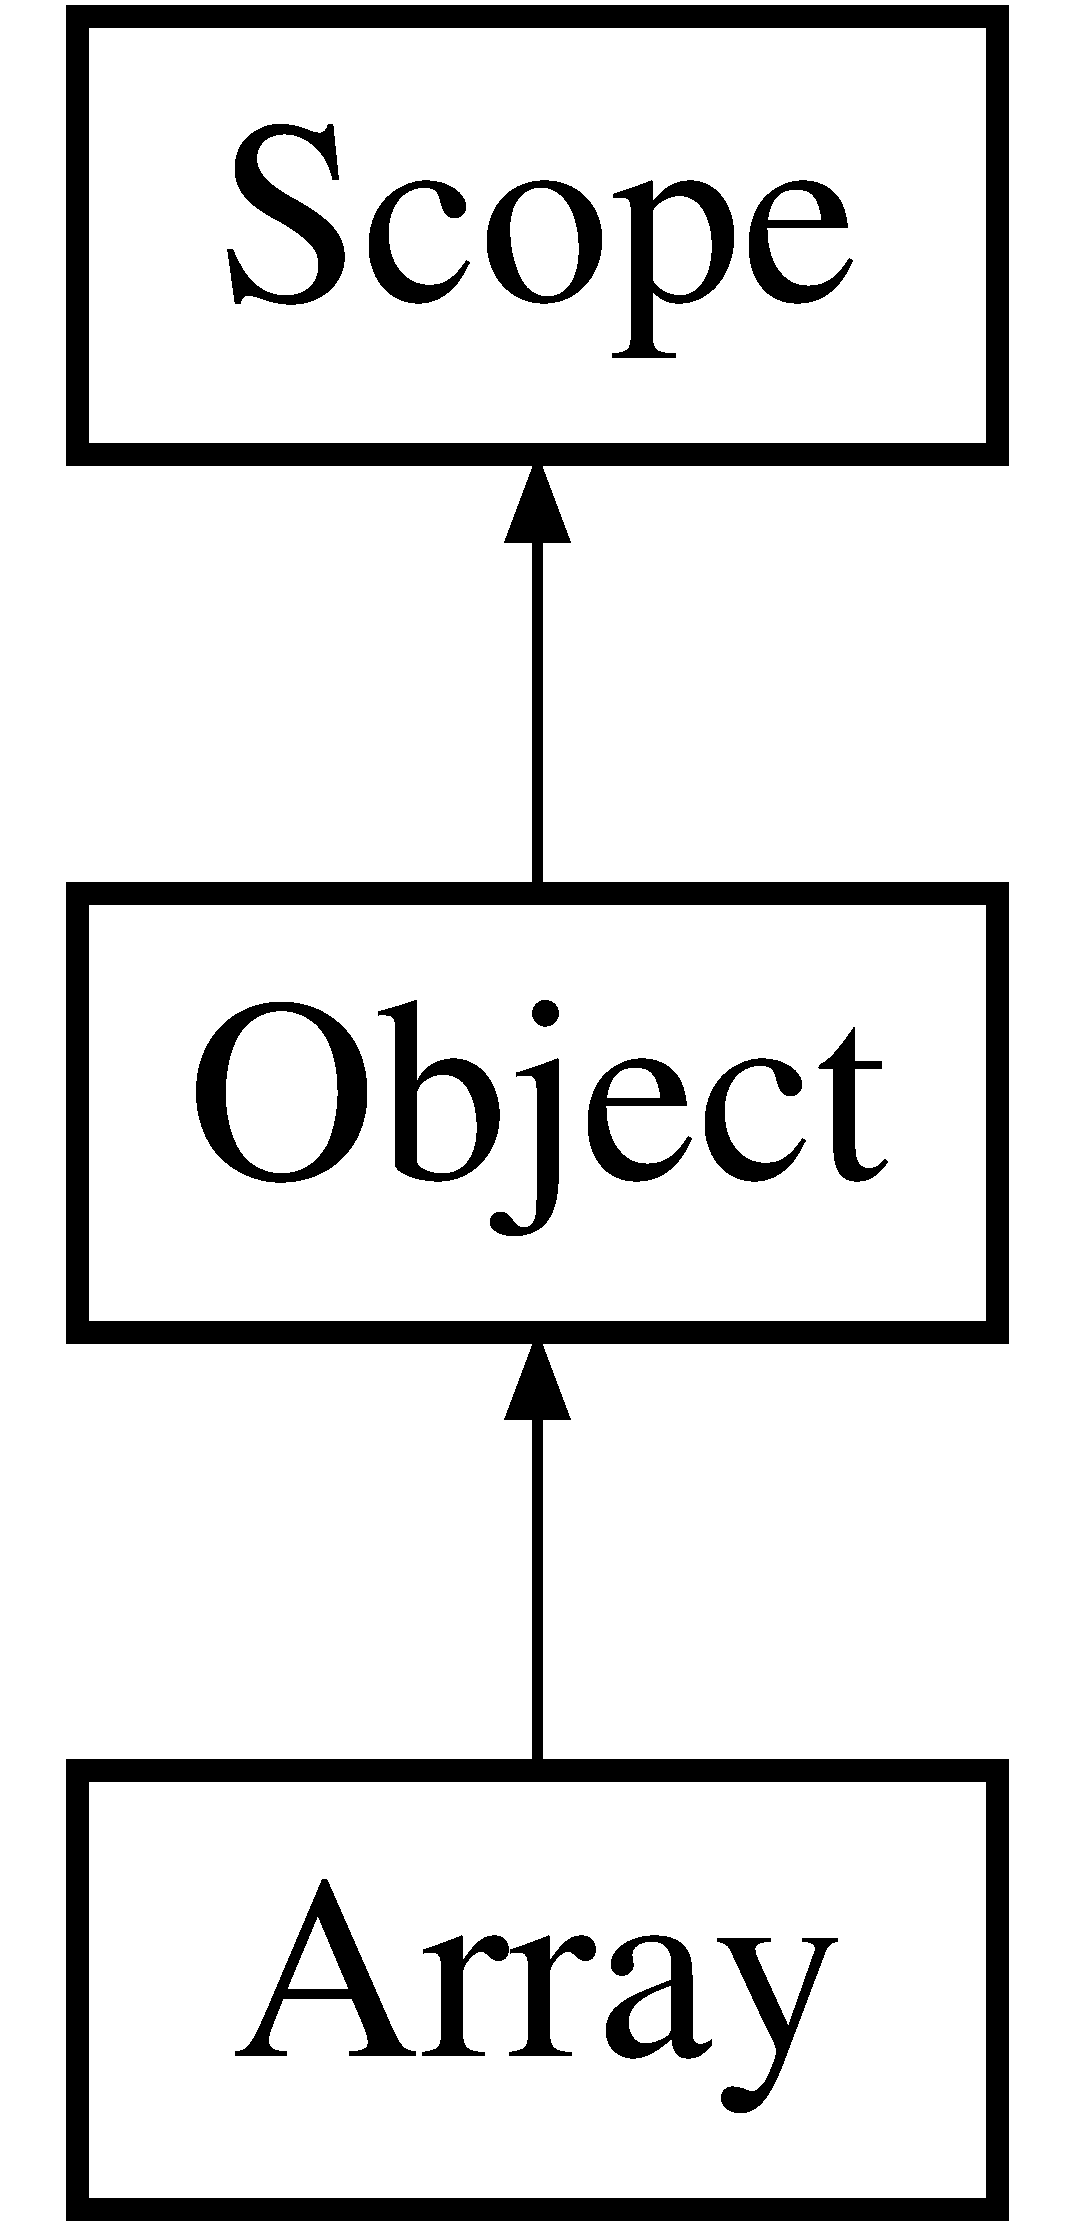
\includegraphics[height=3.000000cm]{classScope}
\end{center}
\end{figure}
\subsection*{Public Member Functions}
\begin{DoxyCompactItemize}
\item 
\hyperlink{classScope_a17c806f9852bb4454ed5709564945373}{Scope} ()
\item 
virtual \hyperlink{classScope_af19fa415c0496acf5667982b584c23d3}{$\sim$\+Scope} ()
\item 
virtual void \hyperlink{classScope_a4c2622adf1835753f5233869febd80d4}{register\+Variable} (\hyperlink{classVariable}{Variable} $\ast$variable)
\item 
\hyperlink{classVariable}{Variable} $\ast$ \hyperlink{classScope_a99112eccd8fd60ac511ed9b754268a6d}{create\+Variable} ()
\item 
\hyperlink{classVariable}{Variable} $\ast$ \hyperlink{classScope_aa723099076a40daa24e7818c6dd1c259}{clone\+Create} (\hyperlink{classVariable}{Variable} $\ast$variable)
\item 
\hyperlink{classVariable}{Variable} $\ast$ \hyperlink{classScope_a910e045176dbe71d2260bac3204e47bb}{get\+Variable} (std\+::string variable\+\_\+name)
\item 
\hyperlink{classVariable}{Variable} $\ast$ \hyperlink{classScope_aa6e0e555c44953e4c8eebaa4adba0b1a}{get\+Variable\+Any\+Scope} (std\+::string variable\+\_\+name)
\item 
void \hyperlink{classScope_a5fe1e6e8c81549eec1ff4dfca7001a69}{remove\+Variable} (\hyperlink{classVariable}{Variable} $\ast$variable)
\item 
virtual void \hyperlink{classScope_a4a42aaa7bd341ef07a90ef51860f0a8a}{on\+Enter\+Scope} ()
\item 
virtual void \hyperlink{classScope_acff92230877eb8ff60f27c86ac56e929}{on\+Leave\+Scope} ()
\item 
bool \hyperlink{classScope_a340e72ca6fa7b3b85760e8b13e75fb16}{is\+Nested\+In\+Scope} (\hyperlink{classScope}{Scope} $\ast$scope)
\item 
std\+::vector$<$ \hyperlink{classVariable}{Variable} $\ast$ $>$ \hyperlink{classScope_adb9ef772a81d2d5ce883298e43161a2d}{get\+Variables} ()
\item 
std\+::vector$<$ \hyperlink{classVariable}{Variable} $\ast$ $>$ \hyperlink{classScope_a93fdedbd4bd26e9eceb1a0e367b3785c}{get\+Object\+Variables\+For} (std\+::shared\+\_\+ptr$<$ \hyperlink{classObject}{Object} $>$ object)
\end{DoxyCompactItemize}
\subsection*{Public Attributes}
\begin{DoxyCompactItemize}
\item 
\hyperlink{classScope}{Scope} $\ast$ \hyperlink{classScope_abc7b9357aa6fae81075bca080ea73d5f}{prev}
\end{DoxyCompactItemize}


\subsection{Constructor \& Destructor Documentation}
\mbox{\Hypertarget{classScope_a17c806f9852bb4454ed5709564945373}\label{classScope_a17c806f9852bb4454ed5709564945373}} 
\index{Scope@{Scope}!Scope@{Scope}}
\index{Scope@{Scope}!Scope@{Scope}}
\subsubsection{\texorpdfstring{Scope()}{Scope()}}
{\footnotesize\ttfamily Scope\+::\+Scope (\begin{DoxyParamCaption}{ }\end{DoxyParamCaption})}

\mbox{\Hypertarget{classScope_af19fa415c0496acf5667982b584c23d3}\label{classScope_af19fa415c0496acf5667982b584c23d3}} 
\index{Scope@{Scope}!````~Scope@{$\sim$\+Scope}}
\index{````~Scope@{$\sim$\+Scope}!Scope@{Scope}}
\subsubsection{\texorpdfstring{$\sim$\+Scope()}{~Scope()}}
{\footnotesize\ttfamily virtual Scope\+::$\sim$\+Scope (\begin{DoxyParamCaption}{ }\end{DoxyParamCaption})\hspace{0.3cm}{\ttfamily [virtual]}}



\subsection{Member Function Documentation}
\mbox{\Hypertarget{classScope_aa723099076a40daa24e7818c6dd1c259}\label{classScope_aa723099076a40daa24e7818c6dd1c259}} 
\index{Scope@{Scope}!clone\+Create@{clone\+Create}}
\index{clone\+Create@{clone\+Create}!Scope@{Scope}}
\subsubsection{\texorpdfstring{clone\+Create()}{cloneCreate()}}
{\footnotesize\ttfamily \hyperlink{classVariable}{Variable}$\ast$ Scope\+::clone\+Create (\begin{DoxyParamCaption}\item[{\hyperlink{classVariable}{Variable} $\ast$}]{variable }\end{DoxyParamCaption})}

\mbox{\Hypertarget{classScope_a99112eccd8fd60ac511ed9b754268a6d}\label{classScope_a99112eccd8fd60ac511ed9b754268a6d}} 
\index{Scope@{Scope}!create\+Variable@{create\+Variable}}
\index{create\+Variable@{create\+Variable}!Scope@{Scope}}
\subsubsection{\texorpdfstring{create\+Variable()}{createVariable()}}
{\footnotesize\ttfamily \hyperlink{classVariable}{Variable}$\ast$ Scope\+::create\+Variable (\begin{DoxyParamCaption}{ }\end{DoxyParamCaption})}

\mbox{\Hypertarget{classScope_a93fdedbd4bd26e9eceb1a0e367b3785c}\label{classScope_a93fdedbd4bd26e9eceb1a0e367b3785c}} 
\index{Scope@{Scope}!get\+Object\+Variables\+For@{get\+Object\+Variables\+For}}
\index{get\+Object\+Variables\+For@{get\+Object\+Variables\+For}!Scope@{Scope}}
\subsubsection{\texorpdfstring{get\+Object\+Variables\+For()}{getObjectVariablesFor()}}
{\footnotesize\ttfamily std\+::vector$<$\hyperlink{classVariable}{Variable}$\ast$$>$ Scope\+::get\+Object\+Variables\+For (\begin{DoxyParamCaption}\item[{std\+::shared\+\_\+ptr$<$ \hyperlink{classObject}{Object} $>$}]{object }\end{DoxyParamCaption})}

\mbox{\Hypertarget{classScope_a910e045176dbe71d2260bac3204e47bb}\label{classScope_a910e045176dbe71d2260bac3204e47bb}} 
\index{Scope@{Scope}!get\+Variable@{get\+Variable}}
\index{get\+Variable@{get\+Variable}!Scope@{Scope}}
\subsubsection{\texorpdfstring{get\+Variable()}{getVariable()}}
{\footnotesize\ttfamily \hyperlink{classVariable}{Variable}$\ast$ Scope\+::get\+Variable (\begin{DoxyParamCaption}\item[{std\+::string}]{variable\+\_\+name }\end{DoxyParamCaption})}

\mbox{\Hypertarget{classScope_aa6e0e555c44953e4c8eebaa4adba0b1a}\label{classScope_aa6e0e555c44953e4c8eebaa4adba0b1a}} 
\index{Scope@{Scope}!get\+Variable\+Any\+Scope@{get\+Variable\+Any\+Scope}}
\index{get\+Variable\+Any\+Scope@{get\+Variable\+Any\+Scope}!Scope@{Scope}}
\subsubsection{\texorpdfstring{get\+Variable\+Any\+Scope()}{getVariableAnyScope()}}
{\footnotesize\ttfamily \hyperlink{classVariable}{Variable}$\ast$ Scope\+::get\+Variable\+Any\+Scope (\begin{DoxyParamCaption}\item[{std\+::string}]{variable\+\_\+name }\end{DoxyParamCaption})}

\mbox{\Hypertarget{classScope_adb9ef772a81d2d5ce883298e43161a2d}\label{classScope_adb9ef772a81d2d5ce883298e43161a2d}} 
\index{Scope@{Scope}!get\+Variables@{get\+Variables}}
\index{get\+Variables@{get\+Variables}!Scope@{Scope}}
\subsubsection{\texorpdfstring{get\+Variables()}{getVariables()}}
{\footnotesize\ttfamily std\+::vector$<$\hyperlink{classVariable}{Variable}$\ast$$>$ Scope\+::get\+Variables (\begin{DoxyParamCaption}{ }\end{DoxyParamCaption})}

\mbox{\Hypertarget{classScope_a340e72ca6fa7b3b85760e8b13e75fb16}\label{classScope_a340e72ca6fa7b3b85760e8b13e75fb16}} 
\index{Scope@{Scope}!is\+Nested\+In\+Scope@{is\+Nested\+In\+Scope}}
\index{is\+Nested\+In\+Scope@{is\+Nested\+In\+Scope}!Scope@{Scope}}
\subsubsection{\texorpdfstring{is\+Nested\+In\+Scope()}{isNestedInScope()}}
{\footnotesize\ttfamily bool Scope\+::is\+Nested\+In\+Scope (\begin{DoxyParamCaption}\item[{\hyperlink{classScope}{Scope} $\ast$}]{scope }\end{DoxyParamCaption})}

\mbox{\Hypertarget{classScope_a4a42aaa7bd341ef07a90ef51860f0a8a}\label{classScope_a4a42aaa7bd341ef07a90ef51860f0a8a}} 
\index{Scope@{Scope}!on\+Enter\+Scope@{on\+Enter\+Scope}}
\index{on\+Enter\+Scope@{on\+Enter\+Scope}!Scope@{Scope}}
\subsubsection{\texorpdfstring{on\+Enter\+Scope()}{onEnterScope()}}
{\footnotesize\ttfamily virtual void Scope\+::on\+Enter\+Scope (\begin{DoxyParamCaption}{ }\end{DoxyParamCaption})\hspace{0.3cm}{\ttfamily [virtual]}}



Reimplemented in \hyperlink{classObject_a61b4cd86dd434abf07e3f4d19b5c93eb}{Object}.

\mbox{\Hypertarget{classScope_acff92230877eb8ff60f27c86ac56e929}\label{classScope_acff92230877eb8ff60f27c86ac56e929}} 
\index{Scope@{Scope}!on\+Leave\+Scope@{on\+Leave\+Scope}}
\index{on\+Leave\+Scope@{on\+Leave\+Scope}!Scope@{Scope}}
\subsubsection{\texorpdfstring{on\+Leave\+Scope()}{onLeaveScope()}}
{\footnotesize\ttfamily virtual void Scope\+::on\+Leave\+Scope (\begin{DoxyParamCaption}{ }\end{DoxyParamCaption})\hspace{0.3cm}{\ttfamily [virtual]}}



Reimplemented in \hyperlink{classObject_a54a99563b5936626d47fb1e2f0e13a9c}{Object}.

\mbox{\Hypertarget{classScope_a4c2622adf1835753f5233869febd80d4}\label{classScope_a4c2622adf1835753f5233869febd80d4}} 
\index{Scope@{Scope}!register\+Variable@{register\+Variable}}
\index{register\+Variable@{register\+Variable}!Scope@{Scope}}
\subsubsection{\texorpdfstring{register\+Variable()}{registerVariable()}}
{\footnotesize\ttfamily virtual void Scope\+::register\+Variable (\begin{DoxyParamCaption}\item[{\hyperlink{classVariable}{Variable} $\ast$}]{variable }\end{DoxyParamCaption})\hspace{0.3cm}{\ttfamily [virtual]}}



Reimplemented in \hyperlink{classObject_ad8f3631de109f50f94432ae9e1f7a130}{Object}.

\mbox{\Hypertarget{classScope_a5fe1e6e8c81549eec1ff4dfca7001a69}\label{classScope_a5fe1e6e8c81549eec1ff4dfca7001a69}} 
\index{Scope@{Scope}!remove\+Variable@{remove\+Variable}}
\index{remove\+Variable@{remove\+Variable}!Scope@{Scope}}
\subsubsection{\texorpdfstring{remove\+Variable()}{removeVariable()}}
{\footnotesize\ttfamily void Scope\+::remove\+Variable (\begin{DoxyParamCaption}\item[{\hyperlink{classVariable}{Variable} $\ast$}]{variable }\end{DoxyParamCaption})}



\subsection{Member Data Documentation}
\mbox{\Hypertarget{classScope_abc7b9357aa6fae81075bca080ea73d5f}\label{classScope_abc7b9357aa6fae81075bca080ea73d5f}} 
\index{Scope@{Scope}!prev@{prev}}
\index{prev@{prev}!Scope@{Scope}}
\subsubsection{\texorpdfstring{prev}{prev}}
{\footnotesize\ttfamily \hyperlink{classScope}{Scope}$\ast$ Scope\+::prev}



The documentation for this class was generated from the following file\+:\begin{DoxyCompactItemize}
\item 
include/\hyperlink{scope_8h}{scope.\+h}\end{DoxyCompactItemize}

\hypertarget{classScopeHandler}{}\section{Scope\+Handler Class Reference}
\label{classScopeHandler}\index{Scope\+Handler@{Scope\+Handler}}


{\ttfamily \#include $<$scopehandler.\+h$>$}

Inheritance diagram for Scope\+Handler\+:\begin{figure}[H]
\begin{center}
\leavevmode
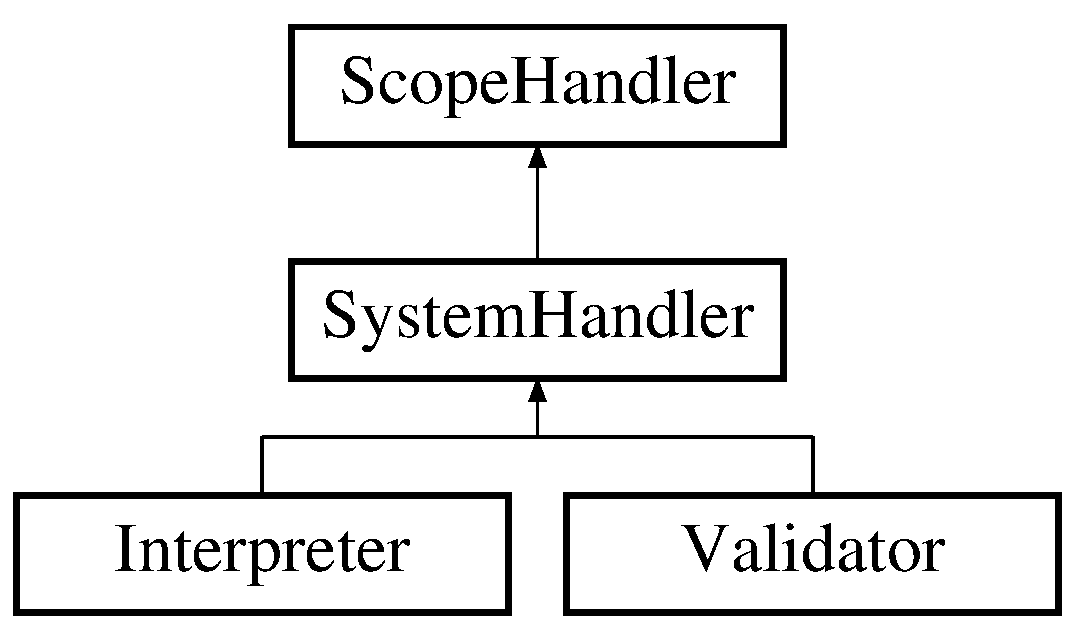
\includegraphics[height=3.000000cm]{classScopeHandler}
\end{center}
\end{figure}
\subsection*{Public Member Functions}
\begin{DoxyCompactItemize}
\item 
\hyperlink{classScopeHandler_a27b5c6a49bda76740ed06114eb250ed1}{Scope\+Handler} ()
\item 
virtual \hyperlink{classScopeHandler_acb1cddd8d15f29d2ce656dff6192c53f}{$\sim$\+Scope\+Handler} ()
\item 
\hyperlink{classScope}{Scope} $\ast$ \hyperlink{classScopeHandler_af6dae9d47ebc9ed6c6931243d2ccee8f}{get\+Current\+Scope} ()
\item 
\hyperlink{classScope}{Scope} $\ast$ \hyperlink{classScopeHandler_af01a4b16265a02b1c786ad54815dd96d}{get\+Root\+Scope} ()
\item 
void \hyperlink{classScopeHandler_a7627747afbebc1dd7017da404fcabd3c}{set\+Current\+Scope} (\hyperlink{classScope}{Scope} $\ast$scope)
\item 
\hyperlink{classScope}{Scope} $\ast$ \hyperlink{classScopeHandler_aabc3a430b566706a8c868a5b1118e37b}{get\+Action\+Scope} ()
\item 
void \hyperlink{classScopeHandler_a9d3db5f048c118eba258981cf04ffd05}{new\+\_\+parented\+\_\+scope} ()
\item 
void \hyperlink{classScopeHandler_a288db413dfebc5a5e18d0cf4ae1b5dfb}{finish\+\_\+parented\+\_\+scope} ()
\item 
\hyperlink{classVariable}{Variable} $\ast$ \hyperlink{classScopeHandler_afd5d7cc4438b75b3ac78e52f1d1779f8}{get\+Variable\+By\+Name} (std\+::string name)
\end{DoxyCompactItemize}


\subsection{Constructor \& Destructor Documentation}
\mbox{\Hypertarget{classScopeHandler_a27b5c6a49bda76740ed06114eb250ed1}\label{classScopeHandler_a27b5c6a49bda76740ed06114eb250ed1}} 
\index{Scope\+Handler@{Scope\+Handler}!Scope\+Handler@{Scope\+Handler}}
\index{Scope\+Handler@{Scope\+Handler}!Scope\+Handler@{Scope\+Handler}}
\subsubsection{\texorpdfstring{Scope\+Handler()}{ScopeHandler()}}
{\footnotesize\ttfamily Scope\+Handler\+::\+Scope\+Handler (\begin{DoxyParamCaption}{ }\end{DoxyParamCaption})}

\mbox{\Hypertarget{classScopeHandler_acb1cddd8d15f29d2ce656dff6192c53f}\label{classScopeHandler_acb1cddd8d15f29d2ce656dff6192c53f}} 
\index{Scope\+Handler@{Scope\+Handler}!````~Scope\+Handler@{$\sim$\+Scope\+Handler}}
\index{````~Scope\+Handler@{$\sim$\+Scope\+Handler}!Scope\+Handler@{Scope\+Handler}}
\subsubsection{\texorpdfstring{$\sim$\+Scope\+Handler()}{~ScopeHandler()}}
{\footnotesize\ttfamily virtual Scope\+Handler\+::$\sim$\+Scope\+Handler (\begin{DoxyParamCaption}{ }\end{DoxyParamCaption})\hspace{0.3cm}{\ttfamily [virtual]}}



\subsection{Member Function Documentation}
\mbox{\Hypertarget{classScopeHandler_a288db413dfebc5a5e18d0cf4ae1b5dfb}\label{classScopeHandler_a288db413dfebc5a5e18d0cf4ae1b5dfb}} 
\index{Scope\+Handler@{Scope\+Handler}!finish\+\_\+parented\+\_\+scope@{finish\+\_\+parented\+\_\+scope}}
\index{finish\+\_\+parented\+\_\+scope@{finish\+\_\+parented\+\_\+scope}!Scope\+Handler@{Scope\+Handler}}
\subsubsection{\texorpdfstring{finish\+\_\+parented\+\_\+scope()}{finish\_parented\_scope()}}
{\footnotesize\ttfamily void Scope\+Handler\+::finish\+\_\+parented\+\_\+scope (\begin{DoxyParamCaption}{ }\end{DoxyParamCaption})}

\mbox{\Hypertarget{classScopeHandler_aabc3a430b566706a8c868a5b1118e37b}\label{classScopeHandler_aabc3a430b566706a8c868a5b1118e37b}} 
\index{Scope\+Handler@{Scope\+Handler}!get\+Action\+Scope@{get\+Action\+Scope}}
\index{get\+Action\+Scope@{get\+Action\+Scope}!Scope\+Handler@{Scope\+Handler}}
\subsubsection{\texorpdfstring{get\+Action\+Scope()}{getActionScope()}}
{\footnotesize\ttfamily \hyperlink{classScope}{Scope}$\ast$ Scope\+Handler\+::get\+Action\+Scope (\begin{DoxyParamCaption}{ }\end{DoxyParamCaption})}

\mbox{\Hypertarget{classScopeHandler_af6dae9d47ebc9ed6c6931243d2ccee8f}\label{classScopeHandler_af6dae9d47ebc9ed6c6931243d2ccee8f}} 
\index{Scope\+Handler@{Scope\+Handler}!get\+Current\+Scope@{get\+Current\+Scope}}
\index{get\+Current\+Scope@{get\+Current\+Scope}!Scope\+Handler@{Scope\+Handler}}
\subsubsection{\texorpdfstring{get\+Current\+Scope()}{getCurrentScope()}}
{\footnotesize\ttfamily \hyperlink{classScope}{Scope}$\ast$ Scope\+Handler\+::get\+Current\+Scope (\begin{DoxyParamCaption}{ }\end{DoxyParamCaption})}

\mbox{\Hypertarget{classScopeHandler_af01a4b16265a02b1c786ad54815dd96d}\label{classScopeHandler_af01a4b16265a02b1c786ad54815dd96d}} 
\index{Scope\+Handler@{Scope\+Handler}!get\+Root\+Scope@{get\+Root\+Scope}}
\index{get\+Root\+Scope@{get\+Root\+Scope}!Scope\+Handler@{Scope\+Handler}}
\subsubsection{\texorpdfstring{get\+Root\+Scope()}{getRootScope()}}
{\footnotesize\ttfamily \hyperlink{classScope}{Scope}$\ast$ Scope\+Handler\+::get\+Root\+Scope (\begin{DoxyParamCaption}{ }\end{DoxyParamCaption})}

\mbox{\Hypertarget{classScopeHandler_afd5d7cc4438b75b3ac78e52f1d1779f8}\label{classScopeHandler_afd5d7cc4438b75b3ac78e52f1d1779f8}} 
\index{Scope\+Handler@{Scope\+Handler}!get\+Variable\+By\+Name@{get\+Variable\+By\+Name}}
\index{get\+Variable\+By\+Name@{get\+Variable\+By\+Name}!Scope\+Handler@{Scope\+Handler}}
\subsubsection{\texorpdfstring{get\+Variable\+By\+Name()}{getVariableByName()}}
{\footnotesize\ttfamily \hyperlink{classVariable}{Variable}$\ast$ Scope\+Handler\+::get\+Variable\+By\+Name (\begin{DoxyParamCaption}\item[{std\+::string}]{name }\end{DoxyParamCaption})}

\mbox{\Hypertarget{classScopeHandler_a9d3db5f048c118eba258981cf04ffd05}\label{classScopeHandler_a9d3db5f048c118eba258981cf04ffd05}} 
\index{Scope\+Handler@{Scope\+Handler}!new\+\_\+parented\+\_\+scope@{new\+\_\+parented\+\_\+scope}}
\index{new\+\_\+parented\+\_\+scope@{new\+\_\+parented\+\_\+scope}!Scope\+Handler@{Scope\+Handler}}
\subsubsection{\texorpdfstring{new\+\_\+parented\+\_\+scope()}{new\_parented\_scope()}}
{\footnotesize\ttfamily void Scope\+Handler\+::new\+\_\+parented\+\_\+scope (\begin{DoxyParamCaption}{ }\end{DoxyParamCaption})}

\mbox{\Hypertarget{classScopeHandler_a7627747afbebc1dd7017da404fcabd3c}\label{classScopeHandler_a7627747afbebc1dd7017da404fcabd3c}} 
\index{Scope\+Handler@{Scope\+Handler}!set\+Current\+Scope@{set\+Current\+Scope}}
\index{set\+Current\+Scope@{set\+Current\+Scope}!Scope\+Handler@{Scope\+Handler}}
\subsubsection{\texorpdfstring{set\+Current\+Scope()}{setCurrentScope()}}
{\footnotesize\ttfamily void Scope\+Handler\+::set\+Current\+Scope (\begin{DoxyParamCaption}\item[{\hyperlink{classScope}{Scope} $\ast$}]{scope }\end{DoxyParamCaption})}



The documentation for this class was generated from the following file\+:\begin{DoxyCompactItemize}
\item 
include/\hyperlink{scopehandler_8h}{scopehandler.\+h}\end{DoxyCompactItemize}

\hypertarget{classSharedSelfHoldingPointer}{}\section{Shared\+Self\+Holding\+Pointer$<$ T $>$ Class Template Reference}
\label{classSharedSelfHoldingPointer}\index{Shared\+Self\+Holding\+Pointer$<$ T $>$@{Shared\+Self\+Holding\+Pointer$<$ T $>$}}


{\ttfamily \#include $<$cpointers.\+h$>$}

\subsection*{Public Member Functions}
\begin{DoxyCompactItemize}
\item 
\hyperlink{classSharedSelfHoldingPointer_a4a81e4be5cf4c074d92122b05ef1a7bf}{Shared\+Self\+Holding\+Pointer} ()
\item 
\hyperlink{classSharedSelfHoldingPointer_af7081c7427461f6a84765a5c6373f2d4}{Shared\+Self\+Holding\+Pointer} (T $\ast$value)
\item 
\hyperlink{classSharedSelfHoldingPointer_a95944d9c7dc5d9b8c6a7efd481ac4906}{Shared\+Self\+Holding\+Pointer} (\hyperlink{classSharedSelfHoldingPointer}{Shared\+Self\+Holding\+Pointer}$<$ T $>$ const \&sp)
\item 
\hyperlink{classSharedSelfHoldingPointer_a1f3b14c8c9f032a20304c1d053163dec}{$\sim$\+Shared\+Self\+Holding\+Pointer} ()
\item 
bool \hyperlink{classSharedSelfHoldingPointer_a92698bf43ff7ad98da2c3d8f451c9baf}{is\+\_\+object\+\_\+stored} (T $\ast$address)
\item 
const \hyperlink{classSharedSelfHoldingPointer}{Shared\+Self\+Holding\+Pointer}$<$ T $>$ \& \hyperlink{classSharedSelfHoldingPointer_afc954c0df268b48304658e3cc078a4d8}{operator=} (const \hyperlink{classSharedSelfHoldingPointer}{Shared\+Self\+Holding\+Pointer}$<$ T $>$ \&\&other)
\item 
void \hyperlink{classSharedSelfHoldingPointer_aaa0d7a61277cb3e6040d010f0f805925}{mark\+\_\+points\+\_\+to\+\_\+self} ()
\item 
T \& \hyperlink{classSharedSelfHoldingPointer_a3080f870971ee581429079cd998b466f}{operator$\ast$} ()
\item 
T $\ast$ \hyperlink{classSharedSelfHoldingPointer_a510f0f53ca3c52af77422b12d6e3ffb6}{operator-\/$>$} ()
\item 
int \hyperlink{classSharedSelfHoldingPointer_a09f8385ee224f32cc86261af7a9643b8}{use\+\_\+count} ()
\end{DoxyCompactItemize}


\subsection{Constructor \& Destructor Documentation}
\mbox{\Hypertarget{classSharedSelfHoldingPointer_a4a81e4be5cf4c074d92122b05ef1a7bf}\label{classSharedSelfHoldingPointer_a4a81e4be5cf4c074d92122b05ef1a7bf}} 
\index{Shared\+Self\+Holding\+Pointer@{Shared\+Self\+Holding\+Pointer}!Shared\+Self\+Holding\+Pointer@{Shared\+Self\+Holding\+Pointer}}
\index{Shared\+Self\+Holding\+Pointer@{Shared\+Self\+Holding\+Pointer}!Shared\+Self\+Holding\+Pointer@{Shared\+Self\+Holding\+Pointer}}
\subsubsection{\texorpdfstring{Shared\+Self\+Holding\+Pointer()}{SharedSelfHoldingPointer()}\hspace{0.1cm}{\footnotesize\ttfamily [1/3]}}
{\footnotesize\ttfamily template$<$typename T$>$ \\
\hyperlink{classSharedSelfHoldingPointer}{Shared\+Self\+Holding\+Pointer}$<$ T $>$\+::\hyperlink{classSharedSelfHoldingPointer}{Shared\+Self\+Holding\+Pointer} (\begin{DoxyParamCaption}{ }\end{DoxyParamCaption})\hspace{0.3cm}{\ttfamily [inline]}}

\mbox{\Hypertarget{classSharedSelfHoldingPointer_af7081c7427461f6a84765a5c6373f2d4}\label{classSharedSelfHoldingPointer_af7081c7427461f6a84765a5c6373f2d4}} 
\index{Shared\+Self\+Holding\+Pointer@{Shared\+Self\+Holding\+Pointer}!Shared\+Self\+Holding\+Pointer@{Shared\+Self\+Holding\+Pointer}}
\index{Shared\+Self\+Holding\+Pointer@{Shared\+Self\+Holding\+Pointer}!Shared\+Self\+Holding\+Pointer@{Shared\+Self\+Holding\+Pointer}}
\subsubsection{\texorpdfstring{Shared\+Self\+Holding\+Pointer()}{SharedSelfHoldingPointer()}\hspace{0.1cm}{\footnotesize\ttfamily [2/3]}}
{\footnotesize\ttfamily template$<$typename T$>$ \\
\hyperlink{classSharedSelfHoldingPointer}{Shared\+Self\+Holding\+Pointer}$<$ T $>$\+::\hyperlink{classSharedSelfHoldingPointer}{Shared\+Self\+Holding\+Pointer} (\begin{DoxyParamCaption}\item[{T $\ast$}]{value }\end{DoxyParamCaption})\hspace{0.3cm}{\ttfamily [inline]}}

\mbox{\Hypertarget{classSharedSelfHoldingPointer_a95944d9c7dc5d9b8c6a7efd481ac4906}\label{classSharedSelfHoldingPointer_a95944d9c7dc5d9b8c6a7efd481ac4906}} 
\index{Shared\+Self\+Holding\+Pointer@{Shared\+Self\+Holding\+Pointer}!Shared\+Self\+Holding\+Pointer@{Shared\+Self\+Holding\+Pointer}}
\index{Shared\+Self\+Holding\+Pointer@{Shared\+Self\+Holding\+Pointer}!Shared\+Self\+Holding\+Pointer@{Shared\+Self\+Holding\+Pointer}}
\subsubsection{\texorpdfstring{Shared\+Self\+Holding\+Pointer()}{SharedSelfHoldingPointer()}\hspace{0.1cm}{\footnotesize\ttfamily [3/3]}}
{\footnotesize\ttfamily template$<$typename T$>$ \\
\hyperlink{classSharedSelfHoldingPointer}{Shared\+Self\+Holding\+Pointer}$<$ T $>$\+::\hyperlink{classSharedSelfHoldingPointer}{Shared\+Self\+Holding\+Pointer} (\begin{DoxyParamCaption}\item[{\hyperlink{classSharedSelfHoldingPointer}{Shared\+Self\+Holding\+Pointer}$<$ T $>$ const \&}]{sp }\end{DoxyParamCaption})\hspace{0.3cm}{\ttfamily [inline]}}

\mbox{\Hypertarget{classSharedSelfHoldingPointer_a1f3b14c8c9f032a20304c1d053163dec}\label{classSharedSelfHoldingPointer_a1f3b14c8c9f032a20304c1d053163dec}} 
\index{Shared\+Self\+Holding\+Pointer@{Shared\+Self\+Holding\+Pointer}!````~Shared\+Self\+Holding\+Pointer@{$\sim$\+Shared\+Self\+Holding\+Pointer}}
\index{````~Shared\+Self\+Holding\+Pointer@{$\sim$\+Shared\+Self\+Holding\+Pointer}!Shared\+Self\+Holding\+Pointer@{Shared\+Self\+Holding\+Pointer}}
\subsubsection{\texorpdfstring{$\sim$\+Shared\+Self\+Holding\+Pointer()}{~SharedSelfHoldingPointer()}}
{\footnotesize\ttfamily template$<$typename T$>$ \\
\hyperlink{classSharedSelfHoldingPointer}{Shared\+Self\+Holding\+Pointer}$<$ T $>$\+::$\sim$\hyperlink{classSharedSelfHoldingPointer}{Shared\+Self\+Holding\+Pointer} (\begin{DoxyParamCaption}{ }\end{DoxyParamCaption})\hspace{0.3cm}{\ttfamily [inline]}}



\subsection{Member Function Documentation}
\mbox{\Hypertarget{classSharedSelfHoldingPointer_a92698bf43ff7ad98da2c3d8f451c9baf}\label{classSharedSelfHoldingPointer_a92698bf43ff7ad98da2c3d8f451c9baf}} 
\index{Shared\+Self\+Holding\+Pointer@{Shared\+Self\+Holding\+Pointer}!is\+\_\+object\+\_\+stored@{is\+\_\+object\+\_\+stored}}
\index{is\+\_\+object\+\_\+stored@{is\+\_\+object\+\_\+stored}!Shared\+Self\+Holding\+Pointer@{Shared\+Self\+Holding\+Pointer}}
\subsubsection{\texorpdfstring{is\+\_\+object\+\_\+stored()}{is\_object\_stored()}}
{\footnotesize\ttfamily template$<$typename T$>$ \\
bool \hyperlink{classSharedSelfHoldingPointer}{Shared\+Self\+Holding\+Pointer}$<$ T $>$\+::is\+\_\+object\+\_\+stored (\begin{DoxyParamCaption}\item[{T $\ast$}]{address }\end{DoxyParamCaption})\hspace{0.3cm}{\ttfamily [inline]}}

\mbox{\Hypertarget{classSharedSelfHoldingPointer_aaa0d7a61277cb3e6040d010f0f805925}\label{classSharedSelfHoldingPointer_aaa0d7a61277cb3e6040d010f0f805925}} 
\index{Shared\+Self\+Holding\+Pointer@{Shared\+Self\+Holding\+Pointer}!mark\+\_\+points\+\_\+to\+\_\+self@{mark\+\_\+points\+\_\+to\+\_\+self}}
\index{mark\+\_\+points\+\_\+to\+\_\+self@{mark\+\_\+points\+\_\+to\+\_\+self}!Shared\+Self\+Holding\+Pointer@{Shared\+Self\+Holding\+Pointer}}
\subsubsection{\texorpdfstring{mark\+\_\+points\+\_\+to\+\_\+self()}{mark\_points\_to\_self()}}
{\footnotesize\ttfamily template$<$typename T$>$ \\
void \hyperlink{classSharedSelfHoldingPointer}{Shared\+Self\+Holding\+Pointer}$<$ T $>$\+::mark\+\_\+points\+\_\+to\+\_\+self (\begin{DoxyParamCaption}{ }\end{DoxyParamCaption})\hspace{0.3cm}{\ttfamily [inline]}}

\mbox{\Hypertarget{classSharedSelfHoldingPointer_a3080f870971ee581429079cd998b466f}\label{classSharedSelfHoldingPointer_a3080f870971ee581429079cd998b466f}} 
\index{Shared\+Self\+Holding\+Pointer@{Shared\+Self\+Holding\+Pointer}!operator$\ast$@{operator$\ast$}}
\index{operator$\ast$@{operator$\ast$}!Shared\+Self\+Holding\+Pointer@{Shared\+Self\+Holding\+Pointer}}
\subsubsection{\texorpdfstring{operator$\ast$()}{operator*()}}
{\footnotesize\ttfamily template$<$typename T$>$ \\
T\& \hyperlink{classSharedSelfHoldingPointer}{Shared\+Self\+Holding\+Pointer}$<$ T $>$\+::operator$\ast$ (\begin{DoxyParamCaption}{ }\end{DoxyParamCaption})\hspace{0.3cm}{\ttfamily [inline]}}

\mbox{\Hypertarget{classSharedSelfHoldingPointer_a510f0f53ca3c52af77422b12d6e3ffb6}\label{classSharedSelfHoldingPointer_a510f0f53ca3c52af77422b12d6e3ffb6}} 
\index{Shared\+Self\+Holding\+Pointer@{Shared\+Self\+Holding\+Pointer}!operator-\/$>$@{operator-\/$>$}}
\index{operator-\/$>$@{operator-\/$>$}!Shared\+Self\+Holding\+Pointer@{Shared\+Self\+Holding\+Pointer}}
\subsubsection{\texorpdfstring{operator-\/$>$()}{operator->()}}
{\footnotesize\ttfamily template$<$typename T$>$ \\
T$\ast$ \hyperlink{classSharedSelfHoldingPointer}{Shared\+Self\+Holding\+Pointer}$<$ T $>$\+::operator-\/$>$ (\begin{DoxyParamCaption}{ }\end{DoxyParamCaption})\hspace{0.3cm}{\ttfamily [inline]}}

\mbox{\Hypertarget{classSharedSelfHoldingPointer_afc954c0df268b48304658e3cc078a4d8}\label{classSharedSelfHoldingPointer_afc954c0df268b48304658e3cc078a4d8}} 
\index{Shared\+Self\+Holding\+Pointer@{Shared\+Self\+Holding\+Pointer}!operator=@{operator=}}
\index{operator=@{operator=}!Shared\+Self\+Holding\+Pointer@{Shared\+Self\+Holding\+Pointer}}
\subsubsection{\texorpdfstring{operator=()}{operator=()}}
{\footnotesize\ttfamily template$<$typename T$>$ \\
const \hyperlink{classSharedSelfHoldingPointer}{Shared\+Self\+Holding\+Pointer}$<$T$>$\& \hyperlink{classSharedSelfHoldingPointer}{Shared\+Self\+Holding\+Pointer}$<$ T $>$\+::operator= (\begin{DoxyParamCaption}\item[{const \hyperlink{classSharedSelfHoldingPointer}{Shared\+Self\+Holding\+Pointer}$<$ T $>$ \&\&}]{other }\end{DoxyParamCaption})\hspace{0.3cm}{\ttfamily [inline]}}

\mbox{\Hypertarget{classSharedSelfHoldingPointer_a09f8385ee224f32cc86261af7a9643b8}\label{classSharedSelfHoldingPointer_a09f8385ee224f32cc86261af7a9643b8}} 
\index{Shared\+Self\+Holding\+Pointer@{Shared\+Self\+Holding\+Pointer}!use\+\_\+count@{use\+\_\+count}}
\index{use\+\_\+count@{use\+\_\+count}!Shared\+Self\+Holding\+Pointer@{Shared\+Self\+Holding\+Pointer}}
\subsubsection{\texorpdfstring{use\+\_\+count()}{use\_count()}}
{\footnotesize\ttfamily template$<$typename T$>$ \\
int \hyperlink{classSharedSelfHoldingPointer}{Shared\+Self\+Holding\+Pointer}$<$ T $>$\+::use\+\_\+count (\begin{DoxyParamCaption}{ }\end{DoxyParamCaption})\hspace{0.3cm}{\ttfamily [inline]}}



The documentation for this class was generated from the following file\+:\begin{DoxyCompactItemize}
\item 
include/\hyperlink{cpointers_8h}{cpointers.\+h}\end{DoxyCompactItemize}

\hypertarget{classSingleFunction}{}\section{Single\+Function Class Reference}
\label{classSingleFunction}\index{Single\+Function@{Single\+Function}}


{\ttfamily \#include $<$singlefunction.\+h$>$}

Inheritance diagram for Single\+Function\+:\begin{figure}[H]
\begin{center}
\leavevmode
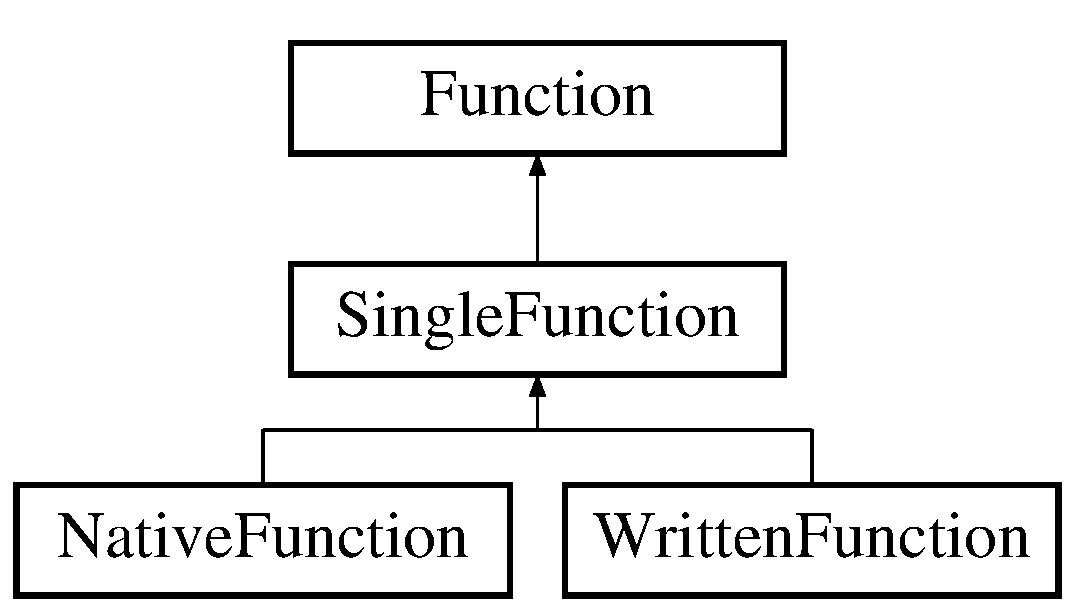
\includegraphics[height=3.000000cm]{classSingleFunction}
\end{center}
\end{figure}
\subsection*{Public Member Functions}
\begin{DoxyCompactItemize}
\item 
\hyperlink{classSingleFunction_a8c6cc400a8f83f317fa62de6886fde40}{Single\+Function} (\hyperlink{statics_8h_a025d9866e39f51183a23b3e2165f0e77}{F\+U\+N\+C\+T\+I\+O\+N\+\_\+\+T\+Y\+PE} \hyperlink{classFunction_a07d7969dbcf44a6a066c6e042a02983d}{type}, std\+::string \hyperlink{classFunction_a161d1ceb4f67f3222caf429fea7b71f1}{name}, std\+::vector$<$ \hyperlink{classVarType}{Var\+Type} $>$ \hyperlink{classSingleFunction_a345cc7c6a42587a62495688af6644a26}{argument\+\_\+types})
\item 
virtual \hyperlink{classSingleFunction_ae414926a60c49b4039e7cd41a304ed77}{$\sim$\+Single\+Function} ()
\end{DoxyCompactItemize}
\subsection*{Public Attributes}
\begin{DoxyCompactItemize}
\item 
std\+::vector$<$ \hyperlink{classVarType}{Var\+Type} $>$ \hyperlink{classSingleFunction_a345cc7c6a42587a62495688af6644a26}{argument\+\_\+types}
\end{DoxyCompactItemize}


\subsection{Constructor \& Destructor Documentation}
\mbox{\Hypertarget{classSingleFunction_a8c6cc400a8f83f317fa62de6886fde40}\label{classSingleFunction_a8c6cc400a8f83f317fa62de6886fde40}} 
\index{Single\+Function@{Single\+Function}!Single\+Function@{Single\+Function}}
\index{Single\+Function@{Single\+Function}!Single\+Function@{Single\+Function}}
\subsubsection{\texorpdfstring{Single\+Function()}{SingleFunction()}}
{\footnotesize\ttfamily Single\+Function\+::\+Single\+Function (\begin{DoxyParamCaption}\item[{\hyperlink{statics_8h_a025d9866e39f51183a23b3e2165f0e77}{F\+U\+N\+C\+T\+I\+O\+N\+\_\+\+T\+Y\+PE}}]{type,  }\item[{std\+::string}]{name,  }\item[{std\+::vector$<$ \hyperlink{classVarType}{Var\+Type} $>$}]{argument\+\_\+types }\end{DoxyParamCaption})}

\mbox{\Hypertarget{classSingleFunction_ae414926a60c49b4039e7cd41a304ed77}\label{classSingleFunction_ae414926a60c49b4039e7cd41a304ed77}} 
\index{Single\+Function@{Single\+Function}!````~Single\+Function@{$\sim$\+Single\+Function}}
\index{````~Single\+Function@{$\sim$\+Single\+Function}!Single\+Function@{Single\+Function}}
\subsubsection{\texorpdfstring{$\sim$\+Single\+Function()}{~SingleFunction()}}
{\footnotesize\ttfamily virtual Single\+Function\+::$\sim$\+Single\+Function (\begin{DoxyParamCaption}{ }\end{DoxyParamCaption})\hspace{0.3cm}{\ttfamily [virtual]}}



\subsection{Member Data Documentation}
\mbox{\Hypertarget{classSingleFunction_a345cc7c6a42587a62495688af6644a26}\label{classSingleFunction_a345cc7c6a42587a62495688af6644a26}} 
\index{Single\+Function@{Single\+Function}!argument\+\_\+types@{argument\+\_\+types}}
\index{argument\+\_\+types@{argument\+\_\+types}!Single\+Function@{Single\+Function}}
\subsubsection{\texorpdfstring{argument\+\_\+types}{argument\_types}}
{\footnotesize\ttfamily std\+::vector$<$\hyperlink{classVarType}{Var\+Type}$>$ Single\+Function\+::argument\+\_\+types}



The documentation for this class was generated from the following file\+:\begin{DoxyCompactItemize}
\item 
include/\hyperlink{singlefunction_8h}{singlefunction.\+h}\end{DoxyCompactItemize}

\hypertarget{structsplit}{}\section{split Struct Reference}
\label{structsplit}\index{split@{split}}


{\ttfamily \#include $<$splitter.\+h$>$}

\subsection*{Public Member Functions}
\begin{DoxyCompactItemize}
\item 
\hyperlink{structsplit_a63f2e1ea2dbcb9973b0f2424c4099d3a}{split} ()
\end{DoxyCompactItemize}
\subsection*{Public Attributes}
\begin{DoxyCompactItemize}
\item 
struct \hyperlink{structoutput__data}{output\+\_\+data} \hyperlink{structsplit_a3efed1338c7ccad093d30c6d94269b6a}{output}
\item 
struct \hyperlink{structmarble__code}{marble\+\_\+code} \hyperlink{structsplit_a8fc2329ce8e3049edfe903fdca076a17}{code}
\item 
bool \hyperlink{structsplit_acc437a097a9733aa0b7c591ec784b271}{has\+\_\+code}
\item 
bool \hyperlink{structsplit_ae2277765e4758fe975c5530dd814c849}{has\+\_\+data}
\item 
bool \hyperlink{structsplit_a13efd7b839008fc3e019b1422fe8ff15}{is\+\_\+last}
\end{DoxyCompactItemize}


\subsection{Constructor \& Destructor Documentation}
\mbox{\Hypertarget{structsplit_a63f2e1ea2dbcb9973b0f2424c4099d3a}\label{structsplit_a63f2e1ea2dbcb9973b0f2424c4099d3a}} 
\index{split@{split}!split@{split}}
\index{split@{split}!split@{split}}
\subsubsection{\texorpdfstring{split()}{split()}}
{\footnotesize\ttfamily split\+::split (\begin{DoxyParamCaption}{ }\end{DoxyParamCaption})}



\subsection{Member Data Documentation}
\mbox{\Hypertarget{structsplit_a8fc2329ce8e3049edfe903fdca076a17}\label{structsplit_a8fc2329ce8e3049edfe903fdca076a17}} 
\index{split@{split}!code@{code}}
\index{code@{code}!split@{split}}
\subsubsection{\texorpdfstring{code}{code}}
{\footnotesize\ttfamily struct \hyperlink{structmarble__code}{marble\+\_\+code} split\+::code}

\mbox{\Hypertarget{structsplit_acc437a097a9733aa0b7c591ec784b271}\label{structsplit_acc437a097a9733aa0b7c591ec784b271}} 
\index{split@{split}!has\+\_\+code@{has\+\_\+code}}
\index{has\+\_\+code@{has\+\_\+code}!split@{split}}
\subsubsection{\texorpdfstring{has\+\_\+code}{has\_code}}
{\footnotesize\ttfamily bool split\+::has\+\_\+code}

\mbox{\Hypertarget{structsplit_ae2277765e4758fe975c5530dd814c849}\label{structsplit_ae2277765e4758fe975c5530dd814c849}} 
\index{split@{split}!has\+\_\+data@{has\+\_\+data}}
\index{has\+\_\+data@{has\+\_\+data}!split@{split}}
\subsubsection{\texorpdfstring{has\+\_\+data}{has\_data}}
{\footnotesize\ttfamily bool split\+::has\+\_\+data}

\mbox{\Hypertarget{structsplit_a13efd7b839008fc3e019b1422fe8ff15}\label{structsplit_a13efd7b839008fc3e019b1422fe8ff15}} 
\index{split@{split}!is\+\_\+last@{is\+\_\+last}}
\index{is\+\_\+last@{is\+\_\+last}!split@{split}}
\subsubsection{\texorpdfstring{is\+\_\+last}{is\_last}}
{\footnotesize\ttfamily bool split\+::is\+\_\+last}

\mbox{\Hypertarget{structsplit_a3efed1338c7ccad093d30c6d94269b6a}\label{structsplit_a3efed1338c7ccad093d30c6d94269b6a}} 
\index{split@{split}!output@{output}}
\index{output@{output}!split@{split}}
\subsubsection{\texorpdfstring{output}{output}}
{\footnotesize\ttfamily struct \hyperlink{structoutput__data}{output\+\_\+data} split\+::output}



The documentation for this struct was generated from the following file\+:\begin{DoxyCompactItemize}
\item 
include/\hyperlink{splitter_8h}{splitter.\+h}\end{DoxyCompactItemize}

\hypertarget{classSplitter}{}\section{Splitter Class Reference}
\label{classSplitter}\index{Splitter@{Splitter}}


{\ttfamily \#include $<$splitter.\+h$>$}

\subsection*{Public Member Functions}
\begin{DoxyCompactItemize}
\item 
\hyperlink{classSplitter_a903043011add23292e7731192a48e768}{Splitter} (\hyperlink{classLogger}{Logger} $\ast$logger, const char $\ast$filename)
\item 
virtual \hyperlink{classSplitter_a39a9ddc7baf2616717677effae5ca547}{$\sim$\+Splitter} ()
\item 
void \hyperlink{classSplitter_a63334af48b3c284b4852af96085a949f}{set\+Data} (const char $\ast$data, int length)
\item 
bool \hyperlink{classSplitter_aec64e7219fdb1aaf94dfcf6b40a03efa}{split} (struct \hyperlink{structsplit}{split} $\ast$\hyperlink{structmarble__code}{marble\+\_\+code})
\end{DoxyCompactItemize}


\subsection{Constructor \& Destructor Documentation}
\mbox{\Hypertarget{classSplitter_a903043011add23292e7731192a48e768}\label{classSplitter_a903043011add23292e7731192a48e768}} 
\index{Splitter@{Splitter}!Splitter@{Splitter}}
\index{Splitter@{Splitter}!Splitter@{Splitter}}
\subsubsection{\texorpdfstring{Splitter()}{Splitter()}}
{\footnotesize\ttfamily Splitter\+::\+Splitter (\begin{DoxyParamCaption}\item[{\hyperlink{classLogger}{Logger} $\ast$}]{logger,  }\item[{const char $\ast$}]{filename }\end{DoxyParamCaption})}

\mbox{\Hypertarget{classSplitter_a39a9ddc7baf2616717677effae5ca547}\label{classSplitter_a39a9ddc7baf2616717677effae5ca547}} 
\index{Splitter@{Splitter}!````~Splitter@{$\sim$\+Splitter}}
\index{````~Splitter@{$\sim$\+Splitter}!Splitter@{Splitter}}
\subsubsection{\texorpdfstring{$\sim$\+Splitter()}{~Splitter()}}
{\footnotesize\ttfamily virtual Splitter\+::$\sim$\+Splitter (\begin{DoxyParamCaption}{ }\end{DoxyParamCaption})\hspace{0.3cm}{\ttfamily [virtual]}}



\subsection{Member Function Documentation}
\mbox{\Hypertarget{classSplitter_a63334af48b3c284b4852af96085a949f}\label{classSplitter_a63334af48b3c284b4852af96085a949f}} 
\index{Splitter@{Splitter}!set\+Data@{set\+Data}}
\index{set\+Data@{set\+Data}!Splitter@{Splitter}}
\subsubsection{\texorpdfstring{set\+Data()}{setData()}}
{\footnotesize\ttfamily void Splitter\+::set\+Data (\begin{DoxyParamCaption}\item[{const char $\ast$}]{data,  }\item[{int}]{length }\end{DoxyParamCaption})}

\mbox{\Hypertarget{classSplitter_aec64e7219fdb1aaf94dfcf6b40a03efa}\label{classSplitter_aec64e7219fdb1aaf94dfcf6b40a03efa}} 
\index{Splitter@{Splitter}!split@{split}}
\index{split@{split}!Splitter@{Splitter}}
\subsubsection{\texorpdfstring{split()}{split()}}
{\footnotesize\ttfamily bool Splitter\+::split (\begin{DoxyParamCaption}\item[{struct \hyperlink{structsplit}{split} $\ast$}]{marble\+\_\+code }\end{DoxyParamCaption})}



The documentation for this class was generated from the following file\+:\begin{DoxyCompactItemize}
\item 
include/\hyperlink{splitter_8h}{splitter.\+h}\end{DoxyCompactItemize}

\hypertarget{classStatement}{}\section{Statement Class Reference}
\label{classStatement}\index{Statement@{Statement}}


{\ttfamily \#include $<$statement.\+h$>$}

Inheritance diagram for Statement\+:\begin{figure}[H]
\begin{center}
\leavevmode
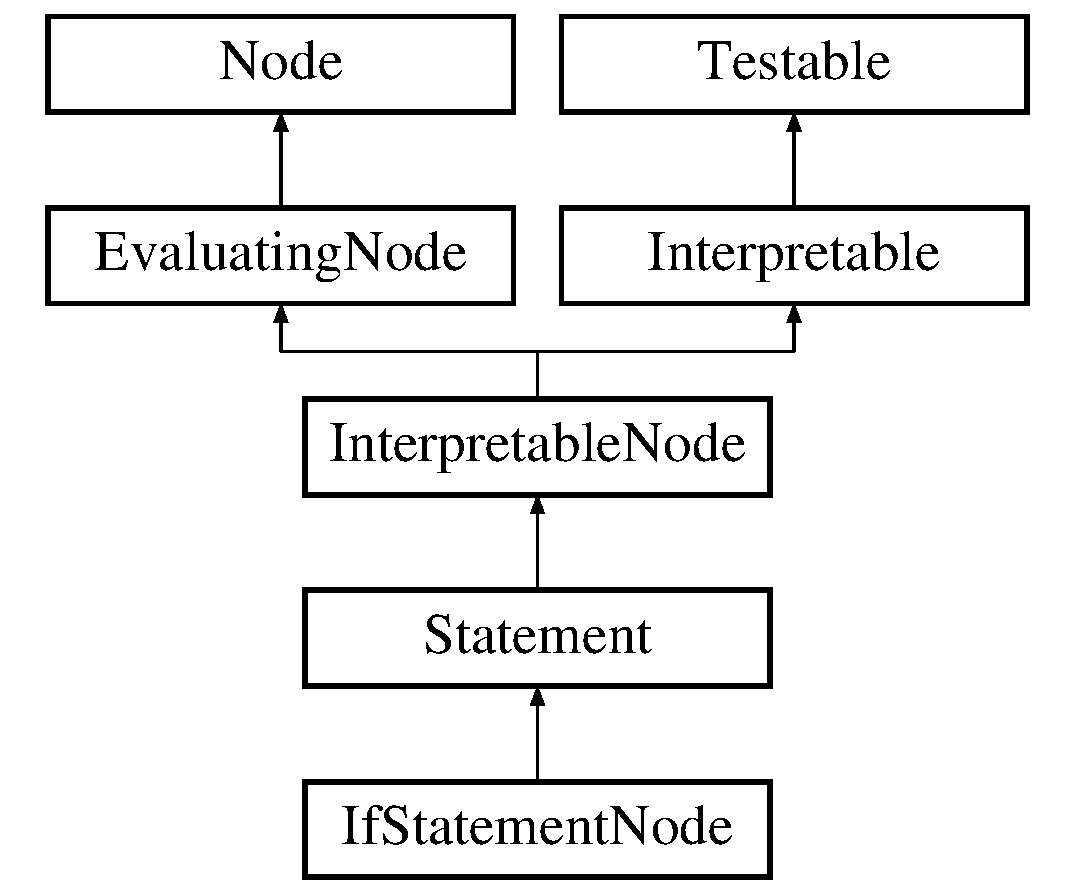
\includegraphics[height=5.000000cm]{classStatement}
\end{center}
\end{figure}
\subsection*{Public Member Functions}
\begin{DoxyCompactItemize}
\item 
\hyperlink{classStatement_a6fb78974779f1f546206a6f301d0fbee}{Statement} (int \hyperlink{classNode_af4f536b1b3f60e197fe364ba56022291}{type})
\item 
virtual \hyperlink{classStatement_aebe8ef20fbd0a932ebb33f6cef555a6d}{$\sim$\+Statement} ()
\end{DoxyCompactItemize}
\subsection*{Public Attributes}
\begin{DoxyCompactItemize}
\item 
\hyperlink{classBodyNode}{Body\+Node} $\ast$ \hyperlink{classStatement_a0aa31d3fbf036cf665062db876341f63}{body}
\end{DoxyCompactItemize}
\subsection*{Additional Inherited Members}


\subsection{Constructor \& Destructor Documentation}
\mbox{\Hypertarget{classStatement_a6fb78974779f1f546206a6f301d0fbee}\label{classStatement_a6fb78974779f1f546206a6f301d0fbee}} 
\index{Statement@{Statement}!Statement@{Statement}}
\index{Statement@{Statement}!Statement@{Statement}}
\subsubsection{\texorpdfstring{Statement()}{Statement()}}
{\footnotesize\ttfamily Statement\+::\+Statement (\begin{DoxyParamCaption}\item[{int}]{type }\end{DoxyParamCaption})}

\mbox{\Hypertarget{classStatement_aebe8ef20fbd0a932ebb33f6cef555a6d}\label{classStatement_aebe8ef20fbd0a932ebb33f6cef555a6d}} 
\index{Statement@{Statement}!````~Statement@{$\sim$\+Statement}}
\index{````~Statement@{$\sim$\+Statement}!Statement@{Statement}}
\subsubsection{\texorpdfstring{$\sim$\+Statement()}{~Statement()}}
{\footnotesize\ttfamily virtual Statement\+::$\sim$\+Statement (\begin{DoxyParamCaption}{ }\end{DoxyParamCaption})\hspace{0.3cm}{\ttfamily [virtual]}}



\subsection{Member Data Documentation}
\mbox{\Hypertarget{classStatement_a0aa31d3fbf036cf665062db876341f63}\label{classStatement_a0aa31d3fbf036cf665062db876341f63}} 
\index{Statement@{Statement}!body@{body}}
\index{body@{body}!Statement@{Statement}}
\subsubsection{\texorpdfstring{body}{body}}
{\footnotesize\ttfamily \hyperlink{classBodyNode}{Body\+Node}$\ast$ Statement\+::body}



The documentation for this class was generated from the following file\+:\begin{DoxyCompactItemize}
\item 
include/\hyperlink{statement_8h}{statement.\+h}\end{DoxyCompactItemize}

\hypertarget{classStringNode}{}\section{String\+Node Class Reference}
\label{classStringNode}\index{String\+Node@{String\+Node}}


{\ttfamily \#include $<$stringnode.\+h$>$}

Inheritance diagram for String\+Node\+:\begin{figure}[H]
\begin{center}
\leavevmode
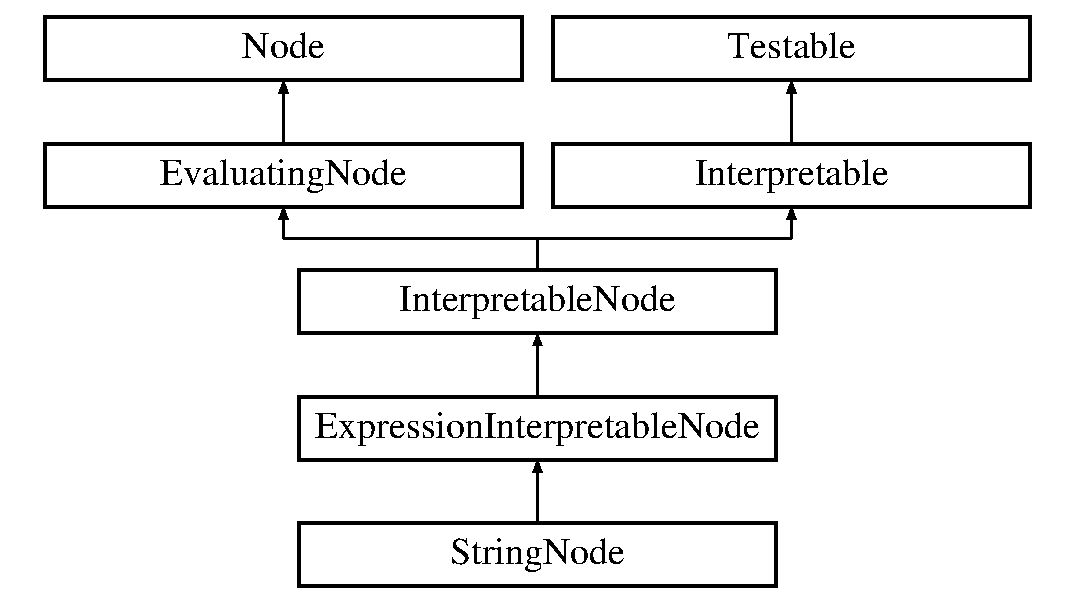
\includegraphics[height=5.000000cm]{classStringNode}
\end{center}
\end{figure}
\subsection*{Public Member Functions}
\begin{DoxyCompactItemize}
\item 
\hyperlink{classStringNode_a3ac1767041e5519e52ada6e7c5ecbbe4}{String\+Node} ()
\item 
virtual \hyperlink{classStringNode_a2b2f8f89db3402822e55da8ede0ca443}{$\sim$\+String\+Node} ()
\item 
virtual void \hyperlink{classStringNode_a3836ad2a1bb6f86cd52663653a65bad8}{test} (\hyperlink{classValidator}{Validator} $\ast$validator)
\item 
virtual \hyperlink{classValue}{Value} \hyperlink{classStringNode_ae92c0858cd07baf0c6417f7bdfce9f0d}{interpret} (\hyperlink{classInterpreter}{Interpreter} $\ast$interpreter)
\item 
virtual void \hyperlink{classStringNode_a1399a24e093f4ecd00957268923c5d23}{evaluate\+\_\+impl} (\hyperlink{classSystemHandler}{System\+Handler} $\ast$handler, \hyperlink{statics_8h_a6664c451ca7787483a7981cc1de68dbb}{E\+V\+A\+L\+U\+A\+T\+I\+O\+N\+\_\+\+T\+Y\+PE} expected\+\_\+evaluation, struct \hyperlink{structEvaluation}{Evaluation} $\ast$evaluation)
\end{DoxyCompactItemize}
\subsection*{Public Attributes}
\begin{DoxyCompactItemize}
\item 
std\+::string \hyperlink{classStringNode_a52fd9cb80da963e39d0d6d33d5396c93}{value}
\end{DoxyCompactItemize}
\subsection*{Additional Inherited Members}


\subsection{Constructor \& Destructor Documentation}
\mbox{\Hypertarget{classStringNode_a3ac1767041e5519e52ada6e7c5ecbbe4}\label{classStringNode_a3ac1767041e5519e52ada6e7c5ecbbe4}} 
\index{String\+Node@{String\+Node}!String\+Node@{String\+Node}}
\index{String\+Node@{String\+Node}!String\+Node@{String\+Node}}
\subsubsection{\texorpdfstring{String\+Node()}{StringNode()}}
{\footnotesize\ttfamily String\+Node\+::\+String\+Node (\begin{DoxyParamCaption}{ }\end{DoxyParamCaption})}

\mbox{\Hypertarget{classStringNode_a2b2f8f89db3402822e55da8ede0ca443}\label{classStringNode_a2b2f8f89db3402822e55da8ede0ca443}} 
\index{String\+Node@{String\+Node}!````~String\+Node@{$\sim$\+String\+Node}}
\index{````~String\+Node@{$\sim$\+String\+Node}!String\+Node@{String\+Node}}
\subsubsection{\texorpdfstring{$\sim$\+String\+Node()}{~StringNode()}}
{\footnotesize\ttfamily virtual String\+Node\+::$\sim$\+String\+Node (\begin{DoxyParamCaption}{ }\end{DoxyParamCaption})\hspace{0.3cm}{\ttfamily [virtual]}}



\subsection{Member Function Documentation}
\mbox{\Hypertarget{classStringNode_a1399a24e093f4ecd00957268923c5d23}\label{classStringNode_a1399a24e093f4ecd00957268923c5d23}} 
\index{String\+Node@{String\+Node}!evaluate\+\_\+impl@{evaluate\+\_\+impl}}
\index{evaluate\+\_\+impl@{evaluate\+\_\+impl}!String\+Node@{String\+Node}}
\subsubsection{\texorpdfstring{evaluate\+\_\+impl()}{evaluate\_impl()}}
{\footnotesize\ttfamily virtual void String\+Node\+::evaluate\+\_\+impl (\begin{DoxyParamCaption}\item[{\hyperlink{classSystemHandler}{System\+Handler} $\ast$}]{handler,  }\item[{\hyperlink{statics_8h_a6664c451ca7787483a7981cc1de68dbb}{E\+V\+A\+L\+U\+A\+T\+I\+O\+N\+\_\+\+T\+Y\+PE}}]{expected\+\_\+evaluation,  }\item[{struct \hyperlink{structEvaluation}{Evaluation} $\ast$}]{evaluation }\end{DoxyParamCaption})\hspace{0.3cm}{\ttfamily [virtual]}}



Implements \hyperlink{classEvaluatingNode_a085fa06e0b46a93c814dc55cda0c1b26}{Evaluating\+Node}.

\mbox{\Hypertarget{classStringNode_ae92c0858cd07baf0c6417f7bdfce9f0d}\label{classStringNode_ae92c0858cd07baf0c6417f7bdfce9f0d}} 
\index{String\+Node@{String\+Node}!interpret@{interpret}}
\index{interpret@{interpret}!String\+Node@{String\+Node}}
\subsubsection{\texorpdfstring{interpret()}{interpret()}}
{\footnotesize\ttfamily virtual \hyperlink{classValue}{Value} String\+Node\+::interpret (\begin{DoxyParamCaption}\item[{\hyperlink{classInterpreter}{Interpreter} $\ast$}]{interpreter }\end{DoxyParamCaption})\hspace{0.3cm}{\ttfamily [virtual]}}



Implements \hyperlink{classExpressionInterpretableNode_a43650f046c48fc539f77a207e3c9181e}{Expression\+Interpretable\+Node}.

\mbox{\Hypertarget{classStringNode_a3836ad2a1bb6f86cd52663653a65bad8}\label{classStringNode_a3836ad2a1bb6f86cd52663653a65bad8}} 
\index{String\+Node@{String\+Node}!test@{test}}
\index{test@{test}!String\+Node@{String\+Node}}
\subsubsection{\texorpdfstring{test()}{test()}}
{\footnotesize\ttfamily virtual void String\+Node\+::test (\begin{DoxyParamCaption}\item[{\hyperlink{classValidator}{Validator} $\ast$}]{validator }\end{DoxyParamCaption})\hspace{0.3cm}{\ttfamily [virtual]}}



Reimplemented from \hyperlink{classInterpretable_a32f547aaf68dcbab993284d3257ab010}{Interpretable}.



\subsection{Member Data Documentation}
\mbox{\Hypertarget{classStringNode_a52fd9cb80da963e39d0d6d33d5396c93}\label{classStringNode_a52fd9cb80da963e39d0d6d33d5396c93}} 
\index{String\+Node@{String\+Node}!value@{value}}
\index{value@{value}!String\+Node@{String\+Node}}
\subsubsection{\texorpdfstring{value}{value}}
{\footnotesize\ttfamily std\+::string String\+Node\+::value}



The documentation for this class was generated from the following file\+:\begin{DoxyCompactItemize}
\item 
include/\hyperlink{stringnode_8h}{stringnode.\+h}\end{DoxyCompactItemize}

\hypertarget{classSystemHandler}{}\section{System\+Handler Class Reference}
\label{classSystemHandler}\index{System\+Handler@{System\+Handler}}


{\ttfamily \#include $<$systemhandler.\+h$>$}

Inheritance diagram for System\+Handler\+:\begin{figure}[H]
\begin{center}
\leavevmode
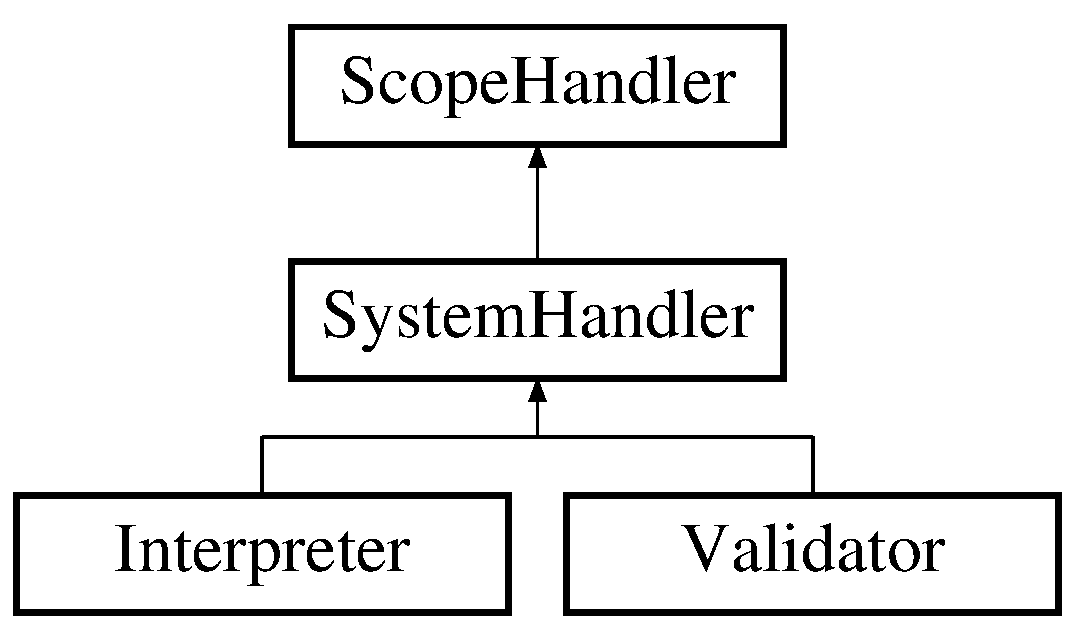
\includegraphics[height=3.000000cm]{classSystemHandler}
\end{center}
\end{figure}
\subsection*{Public Member Functions}
\begin{DoxyCompactItemize}
\item 
\hyperlink{classSystemHandler_abda0d6c76ea3eb8fa8e1493931e5d76b}{System\+Handler} (\hyperlink{statics_8h_a28f867553077bc713fdf8921a9226e2e}{S\+Y\+S\+T\+E\+M\+\_\+\+H\+A\+N\+D\+L\+E\+R\+\_\+\+T\+Y\+PE} \hyperlink{classSystemHandler_a8ca6090af683e8555051681fd31cd865}{type}, \hyperlink{classClassSystem}{Class\+System} $\ast$\hyperlink{classSystemHandler_ab54036ced60be518459b1c4753667912}{base\+Class\+System}, \hyperlink{classFunctionSystem}{Function\+System} $\ast$\hyperlink{classSystemHandler_af601707ec9f56e24be4c0541a1c760f4}{base\+Function\+System})
\item 
virtual \hyperlink{classSystemHandler_afd4662824fbf97d8feb248c346968102}{$\sim$\+System\+Handler} ()
\item 
void \hyperlink{classSystemHandler_af27b9410a75ac02dff13b045afdff038}{set\+Function\+System} (\hyperlink{classFunctionSystem}{Function\+System} $\ast$current\+\_\+fc\+\_\+system)
\item 
\hyperlink{classLogger}{Logger} $\ast$ \hyperlink{classSystemHandler_a2d30e2dd0efb6287ae14b36f1c6bb48b}{get\+Logger} ()
\item 
std\+::shared\+\_\+ptr$<$ \hyperlink{classObject}{Object} $>$ \hyperlink{classSystemHandler_aa2a7dad9232938a79b8a813b1238ee13}{get\+Current\+Object} ()
\item 
void \hyperlink{classSystemHandler_a2954779b7877d67d7207c4ea27194a0c}{set\+Current\+Object} (std\+::shared\+\_\+ptr$<$ \hyperlink{classObject}{Object} $>$ object)
\item 
\hyperlink{classFunctionSystem}{Function\+System} $\ast$ \hyperlink{classSystemHandler_a6622a7fa3c494ec657448d0d3f01eb3b}{get\+Global\+Function\+System} ()
\item 
\hyperlink{classFunctionSystem}{Function\+System} $\ast$ \hyperlink{classSystemHandler_a052dfd8bfff27ed9bf12fd84e066ecb3}{get\+Function\+System} ()
\item 
\hyperlink{classFunctionSystem}{Function\+System} $\ast$ \hyperlink{classSystemHandler_a2013db1f8788be4d7e3eb1da5320de45}{get\+Base\+Function\+System} ()
\item 
\hyperlink{classClassSystem}{Class\+System} $\ast$ \hyperlink{classSystemHandler_a2127b2f17952d52c457d40baa641b009}{get\+Base\+Class\+System} ()
\item 
\hyperlink{classClassSystem}{Class\+System} $\ast$ \hyperlink{classSystemHandler_a218066abe52952bf45c3ba21fdf86368}{get\+Class\+System} ()
\item 
\hyperlink{statics_8h_a28f867553077bc713fdf8921a9226e2e}{S\+Y\+S\+T\+E\+M\+\_\+\+H\+A\+N\+D\+L\+E\+R\+\_\+\+T\+Y\+PE} \hyperlink{classSystemHandler_a7d5df891633958f20c66e8046019bdcb}{get\+Type} ()
\end{DoxyCompactItemize}
\subsection*{Protected Attributes}
\begin{DoxyCompactItemize}
\item 
\hyperlink{classClassSystem}{Class\+System} $\ast$ \hyperlink{classSystemHandler_ab54036ced60be518459b1c4753667912}{base\+Class\+System}
\item 
\hyperlink{classClassSystem}{Class\+System} \hyperlink{classSystemHandler_ace6de39b5621a138654577c93f3ce9aa}{class\+System}
\item 
\hyperlink{classFunctionSystem}{Function\+System} $\ast$ \hyperlink{classSystemHandler_af601707ec9f56e24be4c0541a1c760f4}{base\+Function\+System}
\item 
\hyperlink{classFunctionSystem}{Function\+System} \hyperlink{classSystemHandler_a16b8444f364e1a4dd6db3b210fc8fa4e}{global\+Function\+System}
\item 
\hyperlink{classFunctionSystem}{Function\+System} $\ast$ \hyperlink{classSystemHandler_a5d29f688a621b074c2630470c31e6784}{current\+Function\+System}
\item 
\hyperlink{classLogger}{Logger} \hyperlink{classSystemHandler_aff3c17bc71f072c415a793a6114a5e68}{logger}
\item 
\hyperlink{statics_8h_a28f867553077bc713fdf8921a9226e2e}{S\+Y\+S\+T\+E\+M\+\_\+\+H\+A\+N\+D\+L\+E\+R\+\_\+\+T\+Y\+PE} \hyperlink{classSystemHandler_a8ca6090af683e8555051681fd31cd865}{type}
\item 
std\+::shared\+\_\+ptr$<$ \hyperlink{classObject}{Object} $>$ \hyperlink{classSystemHandler_a069c004c6108de742e7f2d9233c9ee77}{current\+\_\+obj}
\end{DoxyCompactItemize}


\subsection{Constructor \& Destructor Documentation}
\mbox{\Hypertarget{classSystemHandler_abda0d6c76ea3eb8fa8e1493931e5d76b}\label{classSystemHandler_abda0d6c76ea3eb8fa8e1493931e5d76b}} 
\index{System\+Handler@{System\+Handler}!System\+Handler@{System\+Handler}}
\index{System\+Handler@{System\+Handler}!System\+Handler@{System\+Handler}}
\subsubsection{\texorpdfstring{System\+Handler()}{SystemHandler()}}
{\footnotesize\ttfamily System\+Handler\+::\+System\+Handler (\begin{DoxyParamCaption}\item[{\hyperlink{statics_8h_a28f867553077bc713fdf8921a9226e2e}{S\+Y\+S\+T\+E\+M\+\_\+\+H\+A\+N\+D\+L\+E\+R\+\_\+\+T\+Y\+PE}}]{type,  }\item[{\hyperlink{classClassSystem}{Class\+System} $\ast$}]{base\+Class\+System,  }\item[{\hyperlink{classFunctionSystem}{Function\+System} $\ast$}]{base\+Function\+System }\end{DoxyParamCaption})}

\mbox{\Hypertarget{classSystemHandler_afd4662824fbf97d8feb248c346968102}\label{classSystemHandler_afd4662824fbf97d8feb248c346968102}} 
\index{System\+Handler@{System\+Handler}!````~System\+Handler@{$\sim$\+System\+Handler}}
\index{````~System\+Handler@{$\sim$\+System\+Handler}!System\+Handler@{System\+Handler}}
\subsubsection{\texorpdfstring{$\sim$\+System\+Handler()}{~SystemHandler()}}
{\footnotesize\ttfamily virtual System\+Handler\+::$\sim$\+System\+Handler (\begin{DoxyParamCaption}{ }\end{DoxyParamCaption})\hspace{0.3cm}{\ttfamily [virtual]}}



\subsection{Member Function Documentation}
\mbox{\Hypertarget{classSystemHandler_a2127b2f17952d52c457d40baa641b009}\label{classSystemHandler_a2127b2f17952d52c457d40baa641b009}} 
\index{System\+Handler@{System\+Handler}!get\+Base\+Class\+System@{get\+Base\+Class\+System}}
\index{get\+Base\+Class\+System@{get\+Base\+Class\+System}!System\+Handler@{System\+Handler}}
\subsubsection{\texorpdfstring{get\+Base\+Class\+System()}{getBaseClassSystem()}}
{\footnotesize\ttfamily \hyperlink{classClassSystem}{Class\+System}$\ast$ System\+Handler\+::get\+Base\+Class\+System (\begin{DoxyParamCaption}{ }\end{DoxyParamCaption})}

\mbox{\Hypertarget{classSystemHandler_a2013db1f8788be4d7e3eb1da5320de45}\label{classSystemHandler_a2013db1f8788be4d7e3eb1da5320de45}} 
\index{System\+Handler@{System\+Handler}!get\+Base\+Function\+System@{get\+Base\+Function\+System}}
\index{get\+Base\+Function\+System@{get\+Base\+Function\+System}!System\+Handler@{System\+Handler}}
\subsubsection{\texorpdfstring{get\+Base\+Function\+System()}{getBaseFunctionSystem()}}
{\footnotesize\ttfamily \hyperlink{classFunctionSystem}{Function\+System}$\ast$ System\+Handler\+::get\+Base\+Function\+System (\begin{DoxyParamCaption}{ }\end{DoxyParamCaption})}

\mbox{\Hypertarget{classSystemHandler_a218066abe52952bf45c3ba21fdf86368}\label{classSystemHandler_a218066abe52952bf45c3ba21fdf86368}} 
\index{System\+Handler@{System\+Handler}!get\+Class\+System@{get\+Class\+System}}
\index{get\+Class\+System@{get\+Class\+System}!System\+Handler@{System\+Handler}}
\subsubsection{\texorpdfstring{get\+Class\+System()}{getClassSystem()}}
{\footnotesize\ttfamily \hyperlink{classClassSystem}{Class\+System}$\ast$ System\+Handler\+::get\+Class\+System (\begin{DoxyParamCaption}{ }\end{DoxyParamCaption})}

\mbox{\Hypertarget{classSystemHandler_aa2a7dad9232938a79b8a813b1238ee13}\label{classSystemHandler_aa2a7dad9232938a79b8a813b1238ee13}} 
\index{System\+Handler@{System\+Handler}!get\+Current\+Object@{get\+Current\+Object}}
\index{get\+Current\+Object@{get\+Current\+Object}!System\+Handler@{System\+Handler}}
\subsubsection{\texorpdfstring{get\+Current\+Object()}{getCurrentObject()}}
{\footnotesize\ttfamily std\+::shared\+\_\+ptr$<$\hyperlink{classObject}{Object}$>$ System\+Handler\+::get\+Current\+Object (\begin{DoxyParamCaption}{ }\end{DoxyParamCaption})}

\mbox{\Hypertarget{classSystemHandler_a052dfd8bfff27ed9bf12fd84e066ecb3}\label{classSystemHandler_a052dfd8bfff27ed9bf12fd84e066ecb3}} 
\index{System\+Handler@{System\+Handler}!get\+Function\+System@{get\+Function\+System}}
\index{get\+Function\+System@{get\+Function\+System}!System\+Handler@{System\+Handler}}
\subsubsection{\texorpdfstring{get\+Function\+System()}{getFunctionSystem()}}
{\footnotesize\ttfamily \hyperlink{classFunctionSystem}{Function\+System}$\ast$ System\+Handler\+::get\+Function\+System (\begin{DoxyParamCaption}{ }\end{DoxyParamCaption})}

\mbox{\Hypertarget{classSystemHandler_a6622a7fa3c494ec657448d0d3f01eb3b}\label{classSystemHandler_a6622a7fa3c494ec657448d0d3f01eb3b}} 
\index{System\+Handler@{System\+Handler}!get\+Global\+Function\+System@{get\+Global\+Function\+System}}
\index{get\+Global\+Function\+System@{get\+Global\+Function\+System}!System\+Handler@{System\+Handler}}
\subsubsection{\texorpdfstring{get\+Global\+Function\+System()}{getGlobalFunctionSystem()}}
{\footnotesize\ttfamily \hyperlink{classFunctionSystem}{Function\+System}$\ast$ System\+Handler\+::get\+Global\+Function\+System (\begin{DoxyParamCaption}{ }\end{DoxyParamCaption})}

\mbox{\Hypertarget{classSystemHandler_a2d30e2dd0efb6287ae14b36f1c6bb48b}\label{classSystemHandler_a2d30e2dd0efb6287ae14b36f1c6bb48b}} 
\index{System\+Handler@{System\+Handler}!get\+Logger@{get\+Logger}}
\index{get\+Logger@{get\+Logger}!System\+Handler@{System\+Handler}}
\subsubsection{\texorpdfstring{get\+Logger()}{getLogger()}}
{\footnotesize\ttfamily \hyperlink{classLogger}{Logger}$\ast$ System\+Handler\+::get\+Logger (\begin{DoxyParamCaption}{ }\end{DoxyParamCaption})}

\mbox{\Hypertarget{classSystemHandler_a7d5df891633958f20c66e8046019bdcb}\label{classSystemHandler_a7d5df891633958f20c66e8046019bdcb}} 
\index{System\+Handler@{System\+Handler}!get\+Type@{get\+Type}}
\index{get\+Type@{get\+Type}!System\+Handler@{System\+Handler}}
\subsubsection{\texorpdfstring{get\+Type()}{getType()}}
{\footnotesize\ttfamily \hyperlink{statics_8h_a28f867553077bc713fdf8921a9226e2e}{S\+Y\+S\+T\+E\+M\+\_\+\+H\+A\+N\+D\+L\+E\+R\+\_\+\+T\+Y\+PE} System\+Handler\+::get\+Type (\begin{DoxyParamCaption}{ }\end{DoxyParamCaption})}

\mbox{\Hypertarget{classSystemHandler_a2954779b7877d67d7207c4ea27194a0c}\label{classSystemHandler_a2954779b7877d67d7207c4ea27194a0c}} 
\index{System\+Handler@{System\+Handler}!set\+Current\+Object@{set\+Current\+Object}}
\index{set\+Current\+Object@{set\+Current\+Object}!System\+Handler@{System\+Handler}}
\subsubsection{\texorpdfstring{set\+Current\+Object()}{setCurrentObject()}}
{\footnotesize\ttfamily void System\+Handler\+::set\+Current\+Object (\begin{DoxyParamCaption}\item[{std\+::shared\+\_\+ptr$<$ \hyperlink{classObject}{Object} $>$}]{object }\end{DoxyParamCaption})}

\mbox{\Hypertarget{classSystemHandler_af27b9410a75ac02dff13b045afdff038}\label{classSystemHandler_af27b9410a75ac02dff13b045afdff038}} 
\index{System\+Handler@{System\+Handler}!set\+Function\+System@{set\+Function\+System}}
\index{set\+Function\+System@{set\+Function\+System}!System\+Handler@{System\+Handler}}
\subsubsection{\texorpdfstring{set\+Function\+System()}{setFunctionSystem()}}
{\footnotesize\ttfamily void System\+Handler\+::set\+Function\+System (\begin{DoxyParamCaption}\item[{\hyperlink{classFunctionSystem}{Function\+System} $\ast$}]{current\+\_\+fc\+\_\+system }\end{DoxyParamCaption})}



\subsection{Member Data Documentation}
\mbox{\Hypertarget{classSystemHandler_ab54036ced60be518459b1c4753667912}\label{classSystemHandler_ab54036ced60be518459b1c4753667912}} 
\index{System\+Handler@{System\+Handler}!base\+Class\+System@{base\+Class\+System}}
\index{base\+Class\+System@{base\+Class\+System}!System\+Handler@{System\+Handler}}
\subsubsection{\texorpdfstring{base\+Class\+System}{baseClassSystem}}
{\footnotesize\ttfamily \hyperlink{classClassSystem}{Class\+System}$\ast$ System\+Handler\+::base\+Class\+System\hspace{0.3cm}{\ttfamily [protected]}}

\mbox{\Hypertarget{classSystemHandler_af601707ec9f56e24be4c0541a1c760f4}\label{classSystemHandler_af601707ec9f56e24be4c0541a1c760f4}} 
\index{System\+Handler@{System\+Handler}!base\+Function\+System@{base\+Function\+System}}
\index{base\+Function\+System@{base\+Function\+System}!System\+Handler@{System\+Handler}}
\subsubsection{\texorpdfstring{base\+Function\+System}{baseFunctionSystem}}
{\footnotesize\ttfamily \hyperlink{classFunctionSystem}{Function\+System}$\ast$ System\+Handler\+::base\+Function\+System\hspace{0.3cm}{\ttfamily [protected]}}

\mbox{\Hypertarget{classSystemHandler_ace6de39b5621a138654577c93f3ce9aa}\label{classSystemHandler_ace6de39b5621a138654577c93f3ce9aa}} 
\index{System\+Handler@{System\+Handler}!class\+System@{class\+System}}
\index{class\+System@{class\+System}!System\+Handler@{System\+Handler}}
\subsubsection{\texorpdfstring{class\+System}{classSystem}}
{\footnotesize\ttfamily \hyperlink{classClassSystem}{Class\+System} System\+Handler\+::class\+System\hspace{0.3cm}{\ttfamily [protected]}}

\mbox{\Hypertarget{classSystemHandler_a069c004c6108de742e7f2d9233c9ee77}\label{classSystemHandler_a069c004c6108de742e7f2d9233c9ee77}} 
\index{System\+Handler@{System\+Handler}!current\+\_\+obj@{current\+\_\+obj}}
\index{current\+\_\+obj@{current\+\_\+obj}!System\+Handler@{System\+Handler}}
\subsubsection{\texorpdfstring{current\+\_\+obj}{current\_obj}}
{\footnotesize\ttfamily std\+::shared\+\_\+ptr$<$\hyperlink{classObject}{Object}$>$ System\+Handler\+::current\+\_\+obj\hspace{0.3cm}{\ttfamily [protected]}}

\mbox{\Hypertarget{classSystemHandler_a5d29f688a621b074c2630470c31e6784}\label{classSystemHandler_a5d29f688a621b074c2630470c31e6784}} 
\index{System\+Handler@{System\+Handler}!current\+Function\+System@{current\+Function\+System}}
\index{current\+Function\+System@{current\+Function\+System}!System\+Handler@{System\+Handler}}
\subsubsection{\texorpdfstring{current\+Function\+System}{currentFunctionSystem}}
{\footnotesize\ttfamily \hyperlink{classFunctionSystem}{Function\+System}$\ast$ System\+Handler\+::current\+Function\+System\hspace{0.3cm}{\ttfamily [protected]}}

\mbox{\Hypertarget{classSystemHandler_a16b8444f364e1a4dd6db3b210fc8fa4e}\label{classSystemHandler_a16b8444f364e1a4dd6db3b210fc8fa4e}} 
\index{System\+Handler@{System\+Handler}!global\+Function\+System@{global\+Function\+System}}
\index{global\+Function\+System@{global\+Function\+System}!System\+Handler@{System\+Handler}}
\subsubsection{\texorpdfstring{global\+Function\+System}{globalFunctionSystem}}
{\footnotesize\ttfamily \hyperlink{classFunctionSystem}{Function\+System} System\+Handler\+::global\+Function\+System\hspace{0.3cm}{\ttfamily [protected]}}

\mbox{\Hypertarget{classSystemHandler_aff3c17bc71f072c415a793a6114a5e68}\label{classSystemHandler_aff3c17bc71f072c415a793a6114a5e68}} 
\index{System\+Handler@{System\+Handler}!logger@{logger}}
\index{logger@{logger}!System\+Handler@{System\+Handler}}
\subsubsection{\texorpdfstring{logger}{logger}}
{\footnotesize\ttfamily \hyperlink{classLogger}{Logger} System\+Handler\+::logger\hspace{0.3cm}{\ttfamily [protected]}}

\mbox{\Hypertarget{classSystemHandler_a8ca6090af683e8555051681fd31cd865}\label{classSystemHandler_a8ca6090af683e8555051681fd31cd865}} 
\index{System\+Handler@{System\+Handler}!type@{type}}
\index{type@{type}!System\+Handler@{System\+Handler}}
\subsubsection{\texorpdfstring{type}{type}}
{\footnotesize\ttfamily \hyperlink{statics_8h_a28f867553077bc713fdf8921a9226e2e}{S\+Y\+S\+T\+E\+M\+\_\+\+H\+A\+N\+D\+L\+E\+R\+\_\+\+T\+Y\+PE} System\+Handler\+::type\hspace{0.3cm}{\ttfamily [protected]}}



The documentation for this class was generated from the following file\+:\begin{DoxyCompactItemize}
\item 
include/\hyperlink{systemhandler_8h}{systemhandler.\+h}\end{DoxyCompactItemize}

\hypertarget{classTestable}{}\section{Testable Class Reference}
\label{classTestable}\index{Testable@{Testable}}


{\ttfamily \#include $<$testable.\+h$>$}

Inheritance diagram for Testable\+:\begin{figure}[H]
\begin{center}
\leavevmode
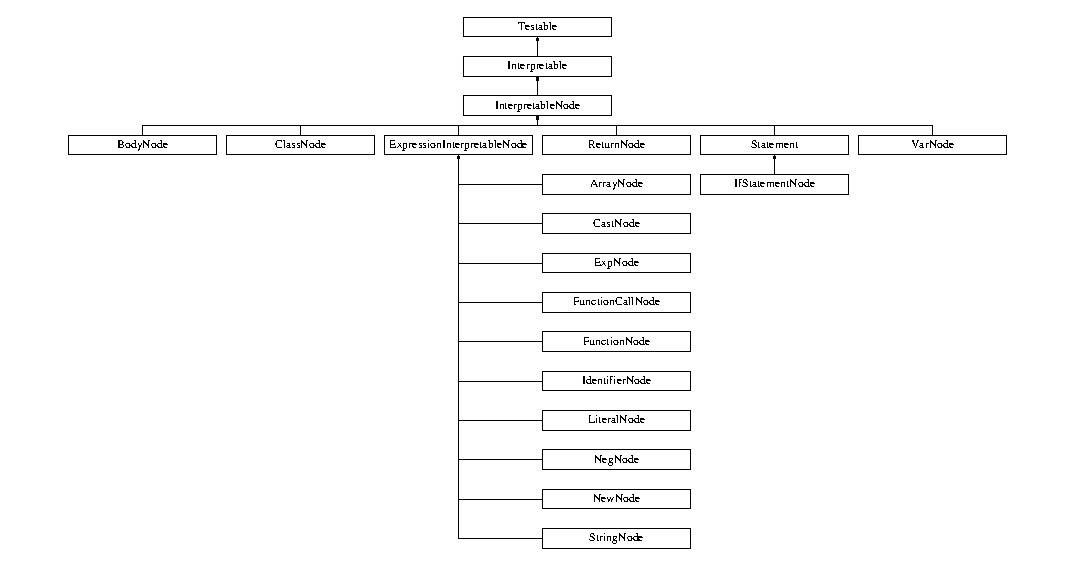
\includegraphics[height=7.140255cm]{classTestable}
\end{center}
\end{figure}
\subsection*{Public Member Functions}
\begin{DoxyCompactItemize}
\item 
virtual void \hyperlink{classTestable_aa10ae4ed84c5d9b36bd69be37790e6ba}{test} (\hyperlink{classValidator}{Validator} $\ast$validator)=0
\end{DoxyCompactItemize}


\subsection{Member Function Documentation}
\mbox{\Hypertarget{classTestable_aa10ae4ed84c5d9b36bd69be37790e6ba}\label{classTestable_aa10ae4ed84c5d9b36bd69be37790e6ba}} 
\index{Testable@{Testable}!test@{test}}
\index{test@{test}!Testable@{Testable}}
\subsubsection{\texorpdfstring{test()}{test()}}
{\footnotesize\ttfamily virtual void Testable\+::test (\begin{DoxyParamCaption}\item[{\hyperlink{classValidator}{Validator} $\ast$}]{validator }\end{DoxyParamCaption})\hspace{0.3cm}{\ttfamily [pure virtual]}}



Implemented in \hyperlink{classNewNode_a9be504d069e8a5d4ea13b4767a3c792a}{New\+Node}, \hyperlink{classVarNode_afaca674319775ae5e8a4fb0e5ec7b59f}{Var\+Node}, \hyperlink{classExpNode_a8fb8302d5ce438a9ad0f58161be2a1c9}{Exp\+Node}, \hyperlink{classFunctionCallNode_a5a7f576984942e2e39057d716d8a5547}{Function\+Call\+Node}, \hyperlink{classFunctionNode_a1f020e7ea0181b3ce16ad2ef8426f773}{Function\+Node}, \hyperlink{classCastNode_a19fa03c324a6dcbadac32965a86afb3e}{Cast\+Node}, \hyperlink{classBodyNode_a80e75b0ab6c388c34a82bdce63fdc7bb}{Body\+Node}, \hyperlink{classInterpretable_a32f547aaf68dcbab993284d3257ab010}{Interpretable}, \hyperlink{classClassNode_ac5147024d81a0c6841e9453025e4f988}{Class\+Node}, \hyperlink{classIdentifierNode_a1459965d8f22ade30cb78b2a1d60dd07}{Identifier\+Node}, \hyperlink{classLiteralNode_af55e4e5e668c9be666c0b6c24c3918f9}{Literal\+Node}, and \hyperlink{classStringNode_a3836ad2a1bb6f86cd52663653a65bad8}{String\+Node}.



The documentation for this class was generated from the following file\+:\begin{DoxyCompactItemize}
\item 
include/\hyperlink{testable_8h}{testable.\+h}\end{DoxyCompactItemize}

\hypertarget{classToken}{}\section{Token Class Reference}
\label{classToken}\index{Token@{Token}}


{\ttfamily \#include $<$token.\+h$>$}

\subsection*{Public Member Functions}
\begin{DoxyCompactItemize}
\item 
\hyperlink{classToken_afe885acc6bfe5ca1d37e3879764a7e20}{Token} (int \hyperlink{classToken_ae46b6b806df89709a13a14dc76c86623}{type}, \hyperlink{classPosInfo}{Pos\+Info} \hyperlink{classToken_a1eea7460906ca57268f808f011af34e6}{pos\+Info})
\item 
virtual \hyperlink{classToken_a40b86b9fc63219310f29413cd89d505a}{$\sim$\+Token} ()
\item 
void \hyperlink{classToken_a6bf54cdc17cec9c64eeefaf756c260d6}{set\+Type} (int \hyperlink{classToken_ae46b6b806df89709a13a14dc76c86623}{type})
\item 
int \hyperlink{classToken_a34e68f22453e7d1d41097ab76ddc199a}{get\+Type} ()
\item 
void \hyperlink{classToken_a0c3a53668483200013e6a2c296fb15c1}{set\+Value} (std\+::string svalue)
\item 
std\+::string \hyperlink{classToken_aeb9ee4b4573bbaab6b33aed601987ff2}{get\+Value} ()
\item 
bool \hyperlink{classToken_aa0b7e4fc76b48f23b0b9cd5daf357f7b}{is\+String} ()
\item 
bool \hyperlink{classToken_a1122d667eaa5a1ae5d5a3b25311693e4}{is\+String} (std\+::string \hyperlink{classToken_a4b7142147b8598f8e24c404928d9263b}{value})
\item 
bool \hyperlink{classToken_a761ab5150b5ecaac78369f25cda2617c}{is\+Symbol} ()
\item 
bool \hyperlink{classToken_ad6a3e5b7a9c56770315cd1c212e634b4}{is\+Symbol} (std\+::string \hyperlink{classToken_a4b7142147b8598f8e24c404928d9263b}{value})
\item 
bool \hyperlink{classToken_ad8fb4783c6e26a402f5d688a0c33075b}{is\+Terminating\+Symbol} ()
\item 
bool \hyperlink{classToken_a12323f98c2de851b0194e7113c28e739}{is\+Castable\+Type} ()
\item 
bool \hyperlink{classToken_ab4d90d6de9f8682d829c4e2461c6aad0}{is\+Identifier} ()
\item 
bool \hyperlink{classToken_a3763eac81818ee9664a67f2b0e058420}{is\+Identifier} (std\+::string \hyperlink{classToken_a4b7142147b8598f8e24c404928d9263b}{value})
\item 
bool \hyperlink{classToken_a5ce5cda79ee936e3c9ff0fb3969420f8}{is\+Keyword} ()
\item 
bool \hyperlink{classToken_a86d5ce12cf462b6621ccc2a8465b5bc0}{is\+Keyword} (std\+::string \hyperlink{classToken_a4b7142147b8598f8e24c404928d9263b}{value})
\item 
bool \hyperlink{classToken_a5392c44a7daf5fba6caa41ce12385a51}{is\+Operator} ()
\item 
bool \hyperlink{classToken_ad7245e07c9d34fa9e9e5f497b221494f}{is\+Operator} (std\+::string \hyperlink{classToken_a4b7142147b8598f8e24c404928d9263b}{value})
\item 
bool \hyperlink{classToken_a4aabdc4152c3a1b000a83488c420a7d3}{is\+Number} ()
\item 
bool \hyperlink{classToken_a4d5ebcf88c3cbfb292fed830172b6e2e}{is\+Number} (std\+::string \hyperlink{classToken_a4b7142147b8598f8e24c404928d9263b}{value})
\item 
bool \hyperlink{classToken_afd50bb7c9ca079392c1edda106bd6345}{is\+Literal} ()
\item 
bool \hyperlink{classToken_a8740433e25b7cc9298c98ce4bac88c42}{is\+Data\+Access\+Keyword} ()
\end{DoxyCompactItemize}
\subsection*{Public Attributes}
\begin{DoxyCompactItemize}
\item 
\hyperlink{classToken}{Token} $\ast$ \hyperlink{classToken_a32f24a25af788c192e5b387dc8d67914}{next}
\item 
int \hyperlink{classToken_ae46b6b806df89709a13a14dc76c86623}{type}
\item 
std\+::string \hyperlink{classToken_a4b7142147b8598f8e24c404928d9263b}{value}
\item 
\hyperlink{classPosInfo}{Pos\+Info} \hyperlink{classToken_a1eea7460906ca57268f808f011af34e6}{pos\+Info}
\end{DoxyCompactItemize}


\subsection{Constructor \& Destructor Documentation}
\mbox{\Hypertarget{classToken_afe885acc6bfe5ca1d37e3879764a7e20}\label{classToken_afe885acc6bfe5ca1d37e3879764a7e20}} 
\index{Token@{Token}!Token@{Token}}
\index{Token@{Token}!Token@{Token}}
\subsubsection{\texorpdfstring{Token()}{Token()}}
{\footnotesize\ttfamily Token\+::\+Token (\begin{DoxyParamCaption}\item[{int}]{type,  }\item[{\hyperlink{classPosInfo}{Pos\+Info}}]{pos\+Info }\end{DoxyParamCaption})}

\mbox{\Hypertarget{classToken_a40b86b9fc63219310f29413cd89d505a}\label{classToken_a40b86b9fc63219310f29413cd89d505a}} 
\index{Token@{Token}!````~Token@{$\sim$\+Token}}
\index{````~Token@{$\sim$\+Token}!Token@{Token}}
\subsubsection{\texorpdfstring{$\sim$\+Token()}{~Token()}}
{\footnotesize\ttfamily virtual Token\+::$\sim$\+Token (\begin{DoxyParamCaption}{ }\end{DoxyParamCaption})\hspace{0.3cm}{\ttfamily [virtual]}}



\subsection{Member Function Documentation}
\mbox{\Hypertarget{classToken_a34e68f22453e7d1d41097ab76ddc199a}\label{classToken_a34e68f22453e7d1d41097ab76ddc199a}} 
\index{Token@{Token}!get\+Type@{get\+Type}}
\index{get\+Type@{get\+Type}!Token@{Token}}
\subsubsection{\texorpdfstring{get\+Type()}{getType()}}
{\footnotesize\ttfamily int Token\+::get\+Type (\begin{DoxyParamCaption}{ }\end{DoxyParamCaption})}

\mbox{\Hypertarget{classToken_aeb9ee4b4573bbaab6b33aed601987ff2}\label{classToken_aeb9ee4b4573bbaab6b33aed601987ff2}} 
\index{Token@{Token}!get\+Value@{get\+Value}}
\index{get\+Value@{get\+Value}!Token@{Token}}
\subsubsection{\texorpdfstring{get\+Value()}{getValue()}}
{\footnotesize\ttfamily std\+::string Token\+::get\+Value (\begin{DoxyParamCaption}{ }\end{DoxyParamCaption})}

\mbox{\Hypertarget{classToken_a12323f98c2de851b0194e7113c28e739}\label{classToken_a12323f98c2de851b0194e7113c28e739}} 
\index{Token@{Token}!is\+Castable\+Type@{is\+Castable\+Type}}
\index{is\+Castable\+Type@{is\+Castable\+Type}!Token@{Token}}
\subsubsection{\texorpdfstring{is\+Castable\+Type()}{isCastableType()}}
{\footnotesize\ttfamily bool Token\+::is\+Castable\+Type (\begin{DoxyParamCaption}{ }\end{DoxyParamCaption})}

\mbox{\Hypertarget{classToken_a8740433e25b7cc9298c98ce4bac88c42}\label{classToken_a8740433e25b7cc9298c98ce4bac88c42}} 
\index{Token@{Token}!is\+Data\+Access\+Keyword@{is\+Data\+Access\+Keyword}}
\index{is\+Data\+Access\+Keyword@{is\+Data\+Access\+Keyword}!Token@{Token}}
\subsubsection{\texorpdfstring{is\+Data\+Access\+Keyword()}{isDataAccessKeyword()}}
{\footnotesize\ttfamily bool Token\+::is\+Data\+Access\+Keyword (\begin{DoxyParamCaption}{ }\end{DoxyParamCaption})}

\mbox{\Hypertarget{classToken_ab4d90d6de9f8682d829c4e2461c6aad0}\label{classToken_ab4d90d6de9f8682d829c4e2461c6aad0}} 
\index{Token@{Token}!is\+Identifier@{is\+Identifier}}
\index{is\+Identifier@{is\+Identifier}!Token@{Token}}
\subsubsection{\texorpdfstring{is\+Identifier()}{isIdentifier()}\hspace{0.1cm}{\footnotesize\ttfamily [1/2]}}
{\footnotesize\ttfamily bool Token\+::is\+Identifier (\begin{DoxyParamCaption}{ }\end{DoxyParamCaption})}

\mbox{\Hypertarget{classToken_a3763eac81818ee9664a67f2b0e058420}\label{classToken_a3763eac81818ee9664a67f2b0e058420}} 
\index{Token@{Token}!is\+Identifier@{is\+Identifier}}
\index{is\+Identifier@{is\+Identifier}!Token@{Token}}
\subsubsection{\texorpdfstring{is\+Identifier()}{isIdentifier()}\hspace{0.1cm}{\footnotesize\ttfamily [2/2]}}
{\footnotesize\ttfamily bool Token\+::is\+Identifier (\begin{DoxyParamCaption}\item[{std\+::string}]{value }\end{DoxyParamCaption})}

\mbox{\Hypertarget{classToken_a5ce5cda79ee936e3c9ff0fb3969420f8}\label{classToken_a5ce5cda79ee936e3c9ff0fb3969420f8}} 
\index{Token@{Token}!is\+Keyword@{is\+Keyword}}
\index{is\+Keyword@{is\+Keyword}!Token@{Token}}
\subsubsection{\texorpdfstring{is\+Keyword()}{isKeyword()}\hspace{0.1cm}{\footnotesize\ttfamily [1/2]}}
{\footnotesize\ttfamily bool Token\+::is\+Keyword (\begin{DoxyParamCaption}{ }\end{DoxyParamCaption})}

\mbox{\Hypertarget{classToken_a86d5ce12cf462b6621ccc2a8465b5bc0}\label{classToken_a86d5ce12cf462b6621ccc2a8465b5bc0}} 
\index{Token@{Token}!is\+Keyword@{is\+Keyword}}
\index{is\+Keyword@{is\+Keyword}!Token@{Token}}
\subsubsection{\texorpdfstring{is\+Keyword()}{isKeyword()}\hspace{0.1cm}{\footnotesize\ttfamily [2/2]}}
{\footnotesize\ttfamily bool Token\+::is\+Keyword (\begin{DoxyParamCaption}\item[{std\+::string}]{value }\end{DoxyParamCaption})}

\mbox{\Hypertarget{classToken_afd50bb7c9ca079392c1edda106bd6345}\label{classToken_afd50bb7c9ca079392c1edda106bd6345}} 
\index{Token@{Token}!is\+Literal@{is\+Literal}}
\index{is\+Literal@{is\+Literal}!Token@{Token}}
\subsubsection{\texorpdfstring{is\+Literal()}{isLiteral()}}
{\footnotesize\ttfamily bool Token\+::is\+Literal (\begin{DoxyParamCaption}{ }\end{DoxyParamCaption})}

\mbox{\Hypertarget{classToken_a4aabdc4152c3a1b000a83488c420a7d3}\label{classToken_a4aabdc4152c3a1b000a83488c420a7d3}} 
\index{Token@{Token}!is\+Number@{is\+Number}}
\index{is\+Number@{is\+Number}!Token@{Token}}
\subsubsection{\texorpdfstring{is\+Number()}{isNumber()}\hspace{0.1cm}{\footnotesize\ttfamily [1/2]}}
{\footnotesize\ttfamily bool Token\+::is\+Number (\begin{DoxyParamCaption}{ }\end{DoxyParamCaption})}

\mbox{\Hypertarget{classToken_a4d5ebcf88c3cbfb292fed830172b6e2e}\label{classToken_a4d5ebcf88c3cbfb292fed830172b6e2e}} 
\index{Token@{Token}!is\+Number@{is\+Number}}
\index{is\+Number@{is\+Number}!Token@{Token}}
\subsubsection{\texorpdfstring{is\+Number()}{isNumber()}\hspace{0.1cm}{\footnotesize\ttfamily [2/2]}}
{\footnotesize\ttfamily bool Token\+::is\+Number (\begin{DoxyParamCaption}\item[{std\+::string}]{value }\end{DoxyParamCaption})}

\mbox{\Hypertarget{classToken_a5392c44a7daf5fba6caa41ce12385a51}\label{classToken_a5392c44a7daf5fba6caa41ce12385a51}} 
\index{Token@{Token}!is\+Operator@{is\+Operator}}
\index{is\+Operator@{is\+Operator}!Token@{Token}}
\subsubsection{\texorpdfstring{is\+Operator()}{isOperator()}\hspace{0.1cm}{\footnotesize\ttfamily [1/2]}}
{\footnotesize\ttfamily bool Token\+::is\+Operator (\begin{DoxyParamCaption}{ }\end{DoxyParamCaption})}

\mbox{\Hypertarget{classToken_ad7245e07c9d34fa9e9e5f497b221494f}\label{classToken_ad7245e07c9d34fa9e9e5f497b221494f}} 
\index{Token@{Token}!is\+Operator@{is\+Operator}}
\index{is\+Operator@{is\+Operator}!Token@{Token}}
\subsubsection{\texorpdfstring{is\+Operator()}{isOperator()}\hspace{0.1cm}{\footnotesize\ttfamily [2/2]}}
{\footnotesize\ttfamily bool Token\+::is\+Operator (\begin{DoxyParamCaption}\item[{std\+::string}]{value }\end{DoxyParamCaption})}

\mbox{\Hypertarget{classToken_aa0b7e4fc76b48f23b0b9cd5daf357f7b}\label{classToken_aa0b7e4fc76b48f23b0b9cd5daf357f7b}} 
\index{Token@{Token}!is\+String@{is\+String}}
\index{is\+String@{is\+String}!Token@{Token}}
\subsubsection{\texorpdfstring{is\+String()}{isString()}\hspace{0.1cm}{\footnotesize\ttfamily [1/2]}}
{\footnotesize\ttfamily bool Token\+::is\+String (\begin{DoxyParamCaption}{ }\end{DoxyParamCaption})}

\mbox{\Hypertarget{classToken_a1122d667eaa5a1ae5d5a3b25311693e4}\label{classToken_a1122d667eaa5a1ae5d5a3b25311693e4}} 
\index{Token@{Token}!is\+String@{is\+String}}
\index{is\+String@{is\+String}!Token@{Token}}
\subsubsection{\texorpdfstring{is\+String()}{isString()}\hspace{0.1cm}{\footnotesize\ttfamily [2/2]}}
{\footnotesize\ttfamily bool Token\+::is\+String (\begin{DoxyParamCaption}\item[{std\+::string}]{value }\end{DoxyParamCaption})}

\mbox{\Hypertarget{classToken_a761ab5150b5ecaac78369f25cda2617c}\label{classToken_a761ab5150b5ecaac78369f25cda2617c}} 
\index{Token@{Token}!is\+Symbol@{is\+Symbol}}
\index{is\+Symbol@{is\+Symbol}!Token@{Token}}
\subsubsection{\texorpdfstring{is\+Symbol()}{isSymbol()}\hspace{0.1cm}{\footnotesize\ttfamily [1/2]}}
{\footnotesize\ttfamily bool Token\+::is\+Symbol (\begin{DoxyParamCaption}{ }\end{DoxyParamCaption})}

\mbox{\Hypertarget{classToken_ad6a3e5b7a9c56770315cd1c212e634b4}\label{classToken_ad6a3e5b7a9c56770315cd1c212e634b4}} 
\index{Token@{Token}!is\+Symbol@{is\+Symbol}}
\index{is\+Symbol@{is\+Symbol}!Token@{Token}}
\subsubsection{\texorpdfstring{is\+Symbol()}{isSymbol()}\hspace{0.1cm}{\footnotesize\ttfamily [2/2]}}
{\footnotesize\ttfamily bool Token\+::is\+Symbol (\begin{DoxyParamCaption}\item[{std\+::string}]{value }\end{DoxyParamCaption})}

\mbox{\Hypertarget{classToken_ad8fb4783c6e26a402f5d688a0c33075b}\label{classToken_ad8fb4783c6e26a402f5d688a0c33075b}} 
\index{Token@{Token}!is\+Terminating\+Symbol@{is\+Terminating\+Symbol}}
\index{is\+Terminating\+Symbol@{is\+Terminating\+Symbol}!Token@{Token}}
\subsubsection{\texorpdfstring{is\+Terminating\+Symbol()}{isTerminatingSymbol()}}
{\footnotesize\ttfamily bool Token\+::is\+Terminating\+Symbol (\begin{DoxyParamCaption}{ }\end{DoxyParamCaption})}

\mbox{\Hypertarget{classToken_a6bf54cdc17cec9c64eeefaf756c260d6}\label{classToken_a6bf54cdc17cec9c64eeefaf756c260d6}} 
\index{Token@{Token}!set\+Type@{set\+Type}}
\index{set\+Type@{set\+Type}!Token@{Token}}
\subsubsection{\texorpdfstring{set\+Type()}{setType()}}
{\footnotesize\ttfamily void Token\+::set\+Type (\begin{DoxyParamCaption}\item[{int}]{type }\end{DoxyParamCaption})}

\mbox{\Hypertarget{classToken_a0c3a53668483200013e6a2c296fb15c1}\label{classToken_a0c3a53668483200013e6a2c296fb15c1}} 
\index{Token@{Token}!set\+Value@{set\+Value}}
\index{set\+Value@{set\+Value}!Token@{Token}}
\subsubsection{\texorpdfstring{set\+Value()}{setValue()}}
{\footnotesize\ttfamily void Token\+::set\+Value (\begin{DoxyParamCaption}\item[{std\+::string}]{svalue }\end{DoxyParamCaption})}



\subsection{Member Data Documentation}
\mbox{\Hypertarget{classToken_a32f24a25af788c192e5b387dc8d67914}\label{classToken_a32f24a25af788c192e5b387dc8d67914}} 
\index{Token@{Token}!next@{next}}
\index{next@{next}!Token@{Token}}
\subsubsection{\texorpdfstring{next}{next}}
{\footnotesize\ttfamily \hyperlink{classToken}{Token}$\ast$ Token\+::next}

\mbox{\Hypertarget{classToken_a1eea7460906ca57268f808f011af34e6}\label{classToken_a1eea7460906ca57268f808f011af34e6}} 
\index{Token@{Token}!pos\+Info@{pos\+Info}}
\index{pos\+Info@{pos\+Info}!Token@{Token}}
\subsubsection{\texorpdfstring{pos\+Info}{posInfo}}
{\footnotesize\ttfamily \hyperlink{classPosInfo}{Pos\+Info} Token\+::pos\+Info}

\mbox{\Hypertarget{classToken_ae46b6b806df89709a13a14dc76c86623}\label{classToken_ae46b6b806df89709a13a14dc76c86623}} 
\index{Token@{Token}!type@{type}}
\index{type@{type}!Token@{Token}}
\subsubsection{\texorpdfstring{type}{type}}
{\footnotesize\ttfamily int Token\+::type}

\mbox{\Hypertarget{classToken_a4b7142147b8598f8e24c404928d9263b}\label{classToken_a4b7142147b8598f8e24c404928d9263b}} 
\index{Token@{Token}!value@{value}}
\index{value@{value}!Token@{Token}}
\subsubsection{\texorpdfstring{value}{value}}
{\footnotesize\ttfamily std\+::string Token\+::value}



The documentation for this class was generated from the following file\+:\begin{DoxyCompactItemize}
\item 
include/\hyperlink{token_8h}{token.\+h}\end{DoxyCompactItemize}

\hypertarget{classTokenFactory}{}\section{Token\+Factory Class Reference}
\label{classTokenFactory}\index{Token\+Factory@{Token\+Factory}}


{\ttfamily \#include $<$tokenfactory.\+h$>$}

\subsection*{Public Member Functions}
\begin{DoxyCompactItemize}
\item 
\hyperlink{classTokenFactory_acacd2ebeaa73671e0f3d7f7110835205}{Token\+Factory} ()
\item 
virtual \hyperlink{classTokenFactory_a5c78c20cdb504edd2003051d7daee759}{$\sim$\+Token\+Factory} ()
\item 
\hyperlink{classToken}{Token} $\ast$ \hyperlink{classTokenFactory_a8cd2afd2f2a645e6ad542a6b10d2ea6b}{create\+Token} (\hyperlink{statics_8h_adb8e9416fa8b5ea4961e9f171db14133}{T\+O\+K\+E\+N\+\_\+\+T\+Y\+PE} token\+\_\+type, \hyperlink{classPosInfo}{Pos\+Info} pos\+Info)
\end{DoxyCompactItemize}


\subsection{Constructor \& Destructor Documentation}
\mbox{\Hypertarget{classTokenFactory_acacd2ebeaa73671e0f3d7f7110835205}\label{classTokenFactory_acacd2ebeaa73671e0f3d7f7110835205}} 
\index{Token\+Factory@{Token\+Factory}!Token\+Factory@{Token\+Factory}}
\index{Token\+Factory@{Token\+Factory}!Token\+Factory@{Token\+Factory}}
\subsubsection{\texorpdfstring{Token\+Factory()}{TokenFactory()}}
{\footnotesize\ttfamily Token\+Factory\+::\+Token\+Factory (\begin{DoxyParamCaption}{ }\end{DoxyParamCaption})}

\mbox{\Hypertarget{classTokenFactory_a5c78c20cdb504edd2003051d7daee759}\label{classTokenFactory_a5c78c20cdb504edd2003051d7daee759}} 
\index{Token\+Factory@{Token\+Factory}!````~Token\+Factory@{$\sim$\+Token\+Factory}}
\index{````~Token\+Factory@{$\sim$\+Token\+Factory}!Token\+Factory@{Token\+Factory}}
\subsubsection{\texorpdfstring{$\sim$\+Token\+Factory()}{~TokenFactory()}}
{\footnotesize\ttfamily virtual Token\+Factory\+::$\sim$\+Token\+Factory (\begin{DoxyParamCaption}{ }\end{DoxyParamCaption})\hspace{0.3cm}{\ttfamily [virtual]}}



\subsection{Member Function Documentation}
\mbox{\Hypertarget{classTokenFactory_a8cd2afd2f2a645e6ad542a6b10d2ea6b}\label{classTokenFactory_a8cd2afd2f2a645e6ad542a6b10d2ea6b}} 
\index{Token\+Factory@{Token\+Factory}!create\+Token@{create\+Token}}
\index{create\+Token@{create\+Token}!Token\+Factory@{Token\+Factory}}
\subsubsection{\texorpdfstring{create\+Token()}{createToken()}}
{\footnotesize\ttfamily \hyperlink{classToken}{Token}$\ast$ Token\+Factory\+::create\+Token (\begin{DoxyParamCaption}\item[{\hyperlink{statics_8h_adb8e9416fa8b5ea4961e9f171db14133}{T\+O\+K\+E\+N\+\_\+\+T\+Y\+PE}}]{token\+\_\+type,  }\item[{\hyperlink{classPosInfo}{Pos\+Info}}]{pos\+Info }\end{DoxyParamCaption})}



The documentation for this class was generated from the following file\+:\begin{DoxyCompactItemize}
\item 
include/\hyperlink{tokenfactory_8h}{tokenfactory.\+h}\end{DoxyCompactItemize}

\hypertarget{classValidator}{}\section{Validator Class Reference}
\label{classValidator}\index{Validator@{Validator}}


{\ttfamily \#include $<$validator.\+h$>$}

Inheritance diagram for Validator\+:\begin{figure}[H]
\begin{center}
\leavevmode
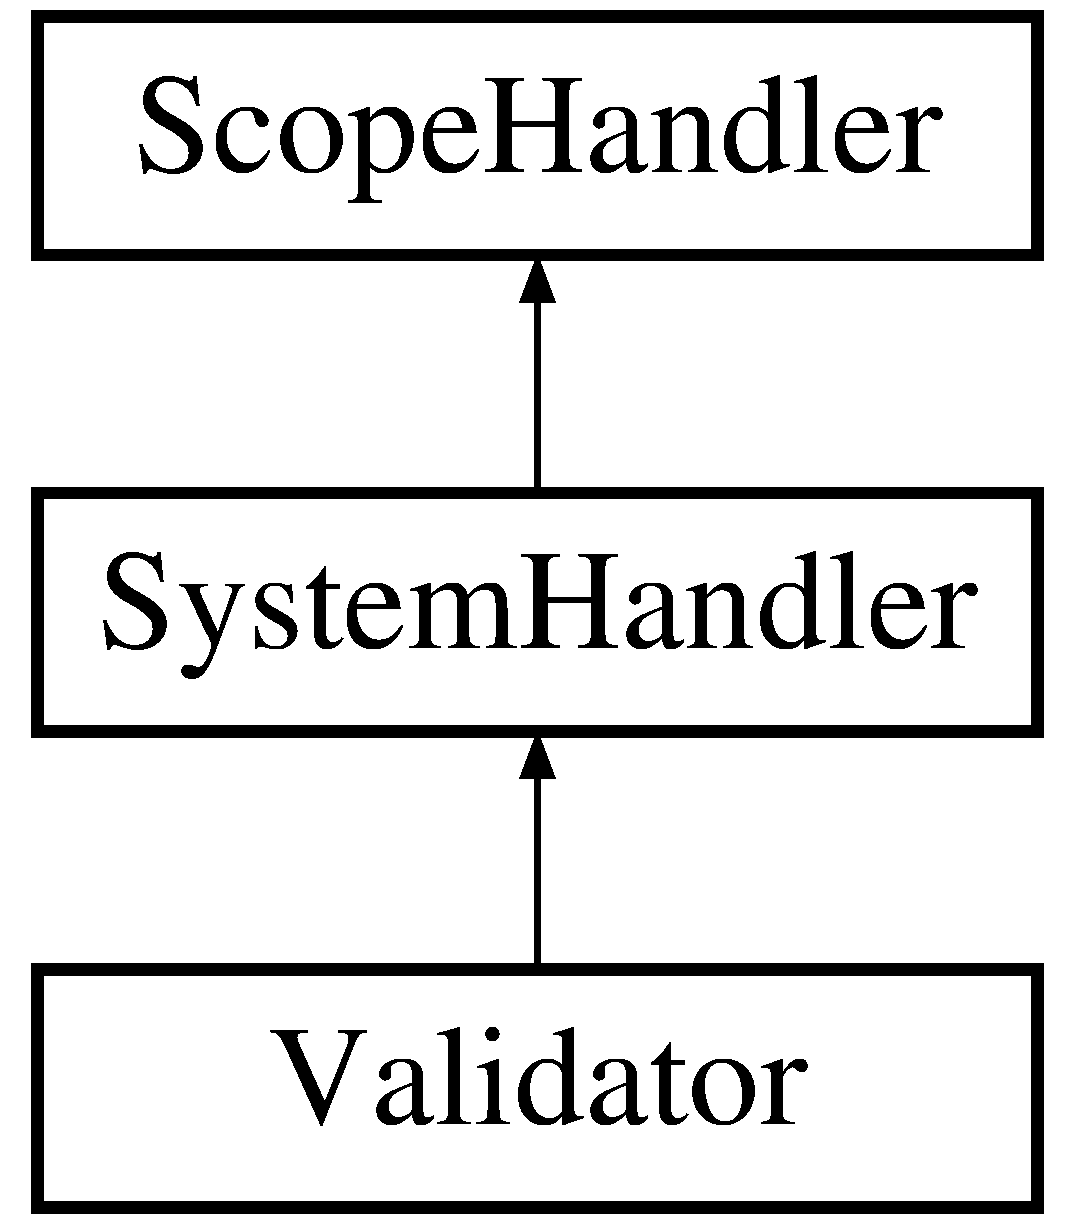
\includegraphics[height=3.000000cm]{classValidator}
\end{center}
\end{figure}
\subsection*{Public Member Functions}
\begin{DoxyCompactItemize}
\item 
\hyperlink{classValidator_a7c66bc9f7104715da531915186691eb8}{Validator} (\hyperlink{classLogger}{Logger} $\ast$logger)
\item 
virtual \hyperlink{classValidator_a4270e7ebf0c451ff80b4ec6fd8eb6a42}{$\sim$\+Validator} ()
\item 
void \hyperlink{classValidator_aa0bc30458ce0255fcec64d8346e384a5}{validate} (\hyperlink{classNode}{Node} $\ast$root\+\_\+node)
\item 
void \hyperlink{classValidator_ad0a3d5e1c57840006e96c74c74eac0aa}{give\+Class\+Object} (std\+::shared\+\_\+ptr$<$ \hyperlink{classObject}{Object} $>$ object)
\item 
\hyperlink{classObject}{Object} $\ast$ \hyperlink{classValidator_afe99d9833e5cda3ab1aab764ab99d716}{get\+Class\+Object} (std\+::string name)
\item 
void \hyperlink{classValidator_a364835c9dc181485838d083b6f227fdb}{begin\+Class} (\hyperlink{classClass}{Class} $\ast$current\+\_\+class)
\item 
\hyperlink{classClass}{Class} $\ast$ \hyperlink{classValidator_a342833ad81caff452754620d29083a3d}{get\+Current\+Class} ()
\item 
void \hyperlink{classValidator_a1d31142fe2275fbc9556d1164b01cbfb}{end\+Class} ()
\item 
void \hyperlink{classValidator_a055e6bdb84438449655135b9166bcf2d}{save} ()
\item 
void \hyperlink{classValidator_a0c89c0c840be87b9011cb518d7bc12ff}{restore} ()
\item 
void \hyperlink{classValidator_a38479b2cec77382e7c25ce898f4d47f9}{expecting} (\hyperlink{statics_8h_a0674a913b8e8c8a9f265baab3646b565}{V\+A\+L\+U\+E\+\_\+\+T\+Y\+PE} \hyperlink{classSystemHandler_a8ca6090af683e8555051681fd31cd865}{type})
\item 
void \hyperlink{classValidator_a6a88dbc8624b8803408094c16a98c205}{expecting\+Object} (std\+::string obj\+\_\+name)
\item 
bool \hyperlink{classValidator_ab94d9925c577be6a8cad24a5a6b60db9}{is\+Expecting} ()
\item 
void \hyperlink{classValidator_adfa1b750001981ae5daa085d32bd626f}{end\+Expecting} ()
\item 
\hyperlink{statics_8h_a0674a913b8e8c8a9f265baab3646b565}{V\+A\+L\+U\+E\+\_\+\+T\+Y\+PE} \hyperlink{classValidator_a786b6b8a5dc6136bbcb2d012e1d8914b}{get\+Expecting\+Type} ()
\item 
std\+::string \hyperlink{classValidator_aca02c85892f3c74114fa936bad41ff07}{get\+Expecting\+Object} ()
\end{DoxyCompactItemize}
\subsection*{Additional Inherited Members}


\subsection{Constructor \& Destructor Documentation}
\mbox{\Hypertarget{classValidator_a7c66bc9f7104715da531915186691eb8}\label{classValidator_a7c66bc9f7104715da531915186691eb8}} 
\index{Validator@{Validator}!Validator@{Validator}}
\index{Validator@{Validator}!Validator@{Validator}}
\subsubsection{\texorpdfstring{Validator()}{Validator()}}
{\footnotesize\ttfamily Validator\+::\+Validator (\begin{DoxyParamCaption}\item[{\hyperlink{classLogger}{Logger} $\ast$}]{logger }\end{DoxyParamCaption})}

\mbox{\Hypertarget{classValidator_a4270e7ebf0c451ff80b4ec6fd8eb6a42}\label{classValidator_a4270e7ebf0c451ff80b4ec6fd8eb6a42}} 
\index{Validator@{Validator}!````~Validator@{$\sim$\+Validator}}
\index{````~Validator@{$\sim$\+Validator}!Validator@{Validator}}
\subsubsection{\texorpdfstring{$\sim$\+Validator()}{~Validator()}}
{\footnotesize\ttfamily virtual Validator\+::$\sim$\+Validator (\begin{DoxyParamCaption}{ }\end{DoxyParamCaption})\hspace{0.3cm}{\ttfamily [virtual]}}



\subsection{Member Function Documentation}
\mbox{\Hypertarget{classValidator_a364835c9dc181485838d083b6f227fdb}\label{classValidator_a364835c9dc181485838d083b6f227fdb}} 
\index{Validator@{Validator}!begin\+Class@{begin\+Class}}
\index{begin\+Class@{begin\+Class}!Validator@{Validator}}
\subsubsection{\texorpdfstring{begin\+Class()}{beginClass()}}
{\footnotesize\ttfamily void Validator\+::begin\+Class (\begin{DoxyParamCaption}\item[{\hyperlink{classClass}{Class} $\ast$}]{current\+\_\+class }\end{DoxyParamCaption})}

\mbox{\Hypertarget{classValidator_a1d31142fe2275fbc9556d1164b01cbfb}\label{classValidator_a1d31142fe2275fbc9556d1164b01cbfb}} 
\index{Validator@{Validator}!end\+Class@{end\+Class}}
\index{end\+Class@{end\+Class}!Validator@{Validator}}
\subsubsection{\texorpdfstring{end\+Class()}{endClass()}}
{\footnotesize\ttfamily void Validator\+::end\+Class (\begin{DoxyParamCaption}{ }\end{DoxyParamCaption})}

\mbox{\Hypertarget{classValidator_adfa1b750001981ae5daa085d32bd626f}\label{classValidator_adfa1b750001981ae5daa085d32bd626f}} 
\index{Validator@{Validator}!end\+Expecting@{end\+Expecting}}
\index{end\+Expecting@{end\+Expecting}!Validator@{Validator}}
\subsubsection{\texorpdfstring{end\+Expecting()}{endExpecting()}}
{\footnotesize\ttfamily void Validator\+::end\+Expecting (\begin{DoxyParamCaption}{ }\end{DoxyParamCaption})}

\mbox{\Hypertarget{classValidator_a38479b2cec77382e7c25ce898f4d47f9}\label{classValidator_a38479b2cec77382e7c25ce898f4d47f9}} 
\index{Validator@{Validator}!expecting@{expecting}}
\index{expecting@{expecting}!Validator@{Validator}}
\subsubsection{\texorpdfstring{expecting()}{expecting()}}
{\footnotesize\ttfamily void Validator\+::expecting (\begin{DoxyParamCaption}\item[{\hyperlink{statics_8h_a0674a913b8e8c8a9f265baab3646b565}{V\+A\+L\+U\+E\+\_\+\+T\+Y\+PE}}]{type }\end{DoxyParamCaption})}

\mbox{\Hypertarget{classValidator_a6a88dbc8624b8803408094c16a98c205}\label{classValidator_a6a88dbc8624b8803408094c16a98c205}} 
\index{Validator@{Validator}!expecting\+Object@{expecting\+Object}}
\index{expecting\+Object@{expecting\+Object}!Validator@{Validator}}
\subsubsection{\texorpdfstring{expecting\+Object()}{expectingObject()}}
{\footnotesize\ttfamily void Validator\+::expecting\+Object (\begin{DoxyParamCaption}\item[{std\+::string}]{obj\+\_\+name }\end{DoxyParamCaption})}

\mbox{\Hypertarget{classValidator_afe99d9833e5cda3ab1aab764ab99d716}\label{classValidator_afe99d9833e5cda3ab1aab764ab99d716}} 
\index{Validator@{Validator}!get\+Class\+Object@{get\+Class\+Object}}
\index{get\+Class\+Object@{get\+Class\+Object}!Validator@{Validator}}
\subsubsection{\texorpdfstring{get\+Class\+Object()}{getClassObject()}}
{\footnotesize\ttfamily \hyperlink{classObject}{Object}$\ast$ Validator\+::get\+Class\+Object (\begin{DoxyParamCaption}\item[{std\+::string}]{name }\end{DoxyParamCaption})}

\mbox{\Hypertarget{classValidator_a342833ad81caff452754620d29083a3d}\label{classValidator_a342833ad81caff452754620d29083a3d}} 
\index{Validator@{Validator}!get\+Current\+Class@{get\+Current\+Class}}
\index{get\+Current\+Class@{get\+Current\+Class}!Validator@{Validator}}
\subsubsection{\texorpdfstring{get\+Current\+Class()}{getCurrentClass()}}
{\footnotesize\ttfamily \hyperlink{classClass}{Class}$\ast$ Validator\+::get\+Current\+Class (\begin{DoxyParamCaption}{ }\end{DoxyParamCaption})}

\mbox{\Hypertarget{classValidator_aca02c85892f3c74114fa936bad41ff07}\label{classValidator_aca02c85892f3c74114fa936bad41ff07}} 
\index{Validator@{Validator}!get\+Expecting\+Object@{get\+Expecting\+Object}}
\index{get\+Expecting\+Object@{get\+Expecting\+Object}!Validator@{Validator}}
\subsubsection{\texorpdfstring{get\+Expecting\+Object()}{getExpectingObject()}}
{\footnotesize\ttfamily std\+::string Validator\+::get\+Expecting\+Object (\begin{DoxyParamCaption}{ }\end{DoxyParamCaption})}

\mbox{\Hypertarget{classValidator_a786b6b8a5dc6136bbcb2d012e1d8914b}\label{classValidator_a786b6b8a5dc6136bbcb2d012e1d8914b}} 
\index{Validator@{Validator}!get\+Expecting\+Type@{get\+Expecting\+Type}}
\index{get\+Expecting\+Type@{get\+Expecting\+Type}!Validator@{Validator}}
\subsubsection{\texorpdfstring{get\+Expecting\+Type()}{getExpectingType()}}
{\footnotesize\ttfamily \hyperlink{statics_8h_a0674a913b8e8c8a9f265baab3646b565}{V\+A\+L\+U\+E\+\_\+\+T\+Y\+PE} Validator\+::get\+Expecting\+Type (\begin{DoxyParamCaption}{ }\end{DoxyParamCaption})}

\mbox{\Hypertarget{classValidator_ad0a3d5e1c57840006e96c74c74eac0aa}\label{classValidator_ad0a3d5e1c57840006e96c74c74eac0aa}} 
\index{Validator@{Validator}!give\+Class\+Object@{give\+Class\+Object}}
\index{give\+Class\+Object@{give\+Class\+Object}!Validator@{Validator}}
\subsubsection{\texorpdfstring{give\+Class\+Object()}{giveClassObject()}}
{\footnotesize\ttfamily void Validator\+::give\+Class\+Object (\begin{DoxyParamCaption}\item[{std\+::shared\+\_\+ptr$<$ \hyperlink{classObject}{Object} $>$}]{object }\end{DoxyParamCaption})}

\mbox{\Hypertarget{classValidator_ab94d9925c577be6a8cad24a5a6b60db9}\label{classValidator_ab94d9925c577be6a8cad24a5a6b60db9}} 
\index{Validator@{Validator}!is\+Expecting@{is\+Expecting}}
\index{is\+Expecting@{is\+Expecting}!Validator@{Validator}}
\subsubsection{\texorpdfstring{is\+Expecting()}{isExpecting()}}
{\footnotesize\ttfamily bool Validator\+::is\+Expecting (\begin{DoxyParamCaption}{ }\end{DoxyParamCaption})}

\mbox{\Hypertarget{classValidator_a0c89c0c840be87b9011cb518d7bc12ff}\label{classValidator_a0c89c0c840be87b9011cb518d7bc12ff}} 
\index{Validator@{Validator}!restore@{restore}}
\index{restore@{restore}!Validator@{Validator}}
\subsubsection{\texorpdfstring{restore()}{restore()}}
{\footnotesize\ttfamily void Validator\+::restore (\begin{DoxyParamCaption}{ }\end{DoxyParamCaption})}

\mbox{\Hypertarget{classValidator_a055e6bdb84438449655135b9166bcf2d}\label{classValidator_a055e6bdb84438449655135b9166bcf2d}} 
\index{Validator@{Validator}!save@{save}}
\index{save@{save}!Validator@{Validator}}
\subsubsection{\texorpdfstring{save()}{save()}}
{\footnotesize\ttfamily void Validator\+::save (\begin{DoxyParamCaption}{ }\end{DoxyParamCaption})}

\mbox{\Hypertarget{classValidator_aa0bc30458ce0255fcec64d8346e384a5}\label{classValidator_aa0bc30458ce0255fcec64d8346e384a5}} 
\index{Validator@{Validator}!validate@{validate}}
\index{validate@{validate}!Validator@{Validator}}
\subsubsection{\texorpdfstring{validate()}{validate()}}
{\footnotesize\ttfamily void Validator\+::validate (\begin{DoxyParamCaption}\item[{\hyperlink{classNode}{Node} $\ast$}]{root\+\_\+node }\end{DoxyParamCaption})}



The documentation for this class was generated from the following file\+:\begin{DoxyCompactItemize}
\item 
include/\hyperlink{validator_8h}{validator.\+h}\end{DoxyCompactItemize}

\hypertarget{classValue}{}\section{Value Class Reference}
\label{classValue}\index{Value@{Value}}


{\ttfamily \#include $<$value.\+h$>$}

\subsection*{Public Member Functions}
\begin{DoxyCompactItemize}
\item 
\hyperlink{classValue_abc2a5a2e6484fac66dae2539cc955667}{Value} ()
\item 
virtual \hyperlink{classValue_aceb26b90be781020c0c71ae5d16ca06f}{$\sim$\+Value} ()
\item 
void \hyperlink{classValue_a83944ac4d53d5bd27fd6a0bd2bc1bd3a}{set} (\hyperlink{classValue}{Value} $\ast$v)
\item 
bool \hyperlink{classValue_a37e1fe6c86dc755a3e000442c4949ab7}{is\+Object\+Or\+Array} ()
\item 
\hyperlink{classValue}{Value} \hyperlink{classValue_a59e467d3ee4cdfb802a2aed8a5a0f1dd}{operator+} (const \hyperlink{classValue}{Value} \&other)
\item 
\hyperlink{classValue}{Value} \hyperlink{classValue_aeb5e368aaea65ed1d1ef37fef6de80fc}{operator-\/} (const \hyperlink{classValue}{Value} \&other)
\item 
\hyperlink{classValue}{Value} \hyperlink{classValue_a8c1b2b5806fbf5d37d0b8bb2ec1ac584}{operator$\ast$} (const \hyperlink{classValue}{Value} \&other)
\item 
\hyperlink{classValue}{Value} \hyperlink{classValue_a5bee3270435124beed9a24cb78941a56}{operator/} (const \hyperlink{classValue}{Value} \&other)
\item 
\hyperlink{classValue}{Value} \hyperlink{classValue_a05800a20d5b799d1a81b28c950899aea}{operator$>$} (const \hyperlink{classValue}{Value} \&other)
\item 
\hyperlink{classValue}{Value} \hyperlink{classValue_ab8f33387ddbc00335cb96643e61643f6}{operator$<$} (const \hyperlink{classValue}{Value} \&other)
\item 
\hyperlink{classValue}{Value} \hyperlink{classValue_a85a296609b51245c4aec34ebf206a66d}{operator$>$=} (const \hyperlink{classValue}{Value} \&other)
\item 
\hyperlink{classValue}{Value} \hyperlink{classValue_a38e0f17676ad08e88bedffb1e931d543}{operator$<$=} (const \hyperlink{classValue}{Value} \&other)
\item 
\hyperlink{classValue}{Value} \hyperlink{classValue_a872c51bf32543279f522426527b4c857}{operator==} (const \hyperlink{classValue}{Value} \&other)
\item 
\hyperlink{classValue}{Value} \hyperlink{classValue_a9ad57dde72c068377e6da67caec558a3}{operator!=} (const \hyperlink{classValue}{Value} \&other)
\item 
\hyperlink{classValue}{Value} \hyperlink{classValue_a8550d0a2396c3222421fdd1aef7ff49b}{operator \&\&} (const \hyperlink{classValue}{Value} \&other)
\item 
\hyperlink{classValue}{Value} \hyperlink{classValue_a2bb40009194bb698b113dc71154d888a}{operator$\vert$$\vert$} (const \hyperlink{classValue}{Value} \&other)
\item 
bool \hyperlink{classValue_a9193333ebda6a44b426ebc24519473db}{has\+Holder} ()
\end{DoxyCompactItemize}
\subsection*{Static Public Member Functions}
\begin{DoxyCompactItemize}
\item 
static \hyperlink{statics_8h_a0674a913b8e8c8a9f265baab3646b565}{V\+A\+L\+U\+E\+\_\+\+T\+Y\+PE} \hyperlink{classValue_a4f772a945a39235b058b18cc187f64a8}{get\+Value\+Type\+For\+String} (std\+::string str)
\item 
static \hyperlink{statics_8h_a0674a913b8e8c8a9f265baab3646b565}{V\+A\+L\+U\+E\+\_\+\+T\+Y\+PE} \hyperlink{classValue_a0fcd69a505d407d2cc8e3095499a9516}{get\+Value\+Type\+From\+Variable\+Type} (\hyperlink{statics_8h_a4c85b3a98d55cc0252806c950379cce0}{V\+A\+R\+I\+A\+B\+L\+E\+\_\+\+T\+Y\+PE} \hyperlink{classValue_a4ee4412ce2c7b78bad42d8eb93294bea}{type})
\item 
static std\+::string \hyperlink{classValue_ad1e0a7607c63edbe77251059d433914e}{get\+Value\+String\+For\+Type} (\hyperlink{statics_8h_a0674a913b8e8c8a9f265baab3646b565}{V\+A\+L\+U\+E\+\_\+\+T\+Y\+PE} \hyperlink{classValue_a4ee4412ce2c7b78bad42d8eb93294bea}{type})
\end{DoxyCompactItemize}
\subsection*{Public Attributes}
\begin{DoxyCompactItemize}
\item 
\hyperlink{statics_8h_a0674a913b8e8c8a9f265baab3646b565}{V\+A\+L\+U\+E\+\_\+\+T\+Y\+PE} \hyperlink{classValue_a4ee4412ce2c7b78bad42d8eb93294bea}{type}
\item 
\hyperlink{classVariable}{Variable} $\ast$ \hyperlink{classValue_af3b547ae64c4985008d6eb7c39868a3f}{holder}
\item 
std\+::string \hyperlink{classValue_a033edf7ba7f753cf274565fac27f9c7d}{svalue}
\item 
\begin{tabbing}
xx\=xx\=xx\=xx\=xx\=xx\=xx\=xx\=xx\=\kill
union \{\\
\>double \hyperlink{classValue_aac350b98b4eb19c6a9b79dae50e97cc6}{dvalue}\\
\>char \hyperlink{classValue_a6690838c4e198bd9b371108cffcd09e3}{bvalue}\\
\}; \\

\end{tabbing}\item 
std\+::shared\+\_\+ptr$<$ \hyperlink{classObject}{Object} $>$ \hyperlink{classValue_a04703ea830e0cb9a24286c588e69ee28}{ovalue}
\item 
std\+::shared\+\_\+ptr$<$ \hyperlink{classArray}{Array} $>$ \hyperlink{classValue_acb0c09facf0b3b0a88f6fb5a240c1783}{avalue}
\end{DoxyCompactItemize}


\subsection{Constructor \& Destructor Documentation}
\mbox{\Hypertarget{classValue_abc2a5a2e6484fac66dae2539cc955667}\label{classValue_abc2a5a2e6484fac66dae2539cc955667}} 
\index{Value@{Value}!Value@{Value}}
\index{Value@{Value}!Value@{Value}}
\subsubsection{\texorpdfstring{Value()}{Value()}}
{\footnotesize\ttfamily Value\+::\+Value (\begin{DoxyParamCaption}{ }\end{DoxyParamCaption})}

\mbox{\Hypertarget{classValue_aceb26b90be781020c0c71ae5d16ca06f}\label{classValue_aceb26b90be781020c0c71ae5d16ca06f}} 
\index{Value@{Value}!````~Value@{$\sim$\+Value}}
\index{````~Value@{$\sim$\+Value}!Value@{Value}}
\subsubsection{\texorpdfstring{$\sim$\+Value()}{~Value()}}
{\footnotesize\ttfamily virtual Value\+::$\sim$\+Value (\begin{DoxyParamCaption}{ }\end{DoxyParamCaption})\hspace{0.3cm}{\ttfamily [virtual]}}



\subsection{Member Function Documentation}
\mbox{\Hypertarget{classValue_ad1e0a7607c63edbe77251059d433914e}\label{classValue_ad1e0a7607c63edbe77251059d433914e}} 
\index{Value@{Value}!get\+Value\+String\+For\+Type@{get\+Value\+String\+For\+Type}}
\index{get\+Value\+String\+For\+Type@{get\+Value\+String\+For\+Type}!Value@{Value}}
\subsubsection{\texorpdfstring{get\+Value\+String\+For\+Type()}{getValueStringForType()}}
{\footnotesize\ttfamily static std\+::string Value\+::get\+Value\+String\+For\+Type (\begin{DoxyParamCaption}\item[{\hyperlink{statics_8h_a0674a913b8e8c8a9f265baab3646b565}{V\+A\+L\+U\+E\+\_\+\+T\+Y\+PE}}]{type }\end{DoxyParamCaption})\hspace{0.3cm}{\ttfamily [static]}}

\mbox{\Hypertarget{classValue_a4f772a945a39235b058b18cc187f64a8}\label{classValue_a4f772a945a39235b058b18cc187f64a8}} 
\index{Value@{Value}!get\+Value\+Type\+For\+String@{get\+Value\+Type\+For\+String}}
\index{get\+Value\+Type\+For\+String@{get\+Value\+Type\+For\+String}!Value@{Value}}
\subsubsection{\texorpdfstring{get\+Value\+Type\+For\+String()}{getValueTypeForString()}}
{\footnotesize\ttfamily static \hyperlink{statics_8h_a0674a913b8e8c8a9f265baab3646b565}{V\+A\+L\+U\+E\+\_\+\+T\+Y\+PE} Value\+::get\+Value\+Type\+For\+String (\begin{DoxyParamCaption}\item[{std\+::string}]{str }\end{DoxyParamCaption})\hspace{0.3cm}{\ttfamily [static]}}

\mbox{\Hypertarget{classValue_a0fcd69a505d407d2cc8e3095499a9516}\label{classValue_a0fcd69a505d407d2cc8e3095499a9516}} 
\index{Value@{Value}!get\+Value\+Type\+From\+Variable\+Type@{get\+Value\+Type\+From\+Variable\+Type}}
\index{get\+Value\+Type\+From\+Variable\+Type@{get\+Value\+Type\+From\+Variable\+Type}!Value@{Value}}
\subsubsection{\texorpdfstring{get\+Value\+Type\+From\+Variable\+Type()}{getValueTypeFromVariableType()}}
{\footnotesize\ttfamily static \hyperlink{statics_8h_a0674a913b8e8c8a9f265baab3646b565}{V\+A\+L\+U\+E\+\_\+\+T\+Y\+PE} Value\+::get\+Value\+Type\+From\+Variable\+Type (\begin{DoxyParamCaption}\item[{\hyperlink{statics_8h_a4c85b3a98d55cc0252806c950379cce0}{V\+A\+R\+I\+A\+B\+L\+E\+\_\+\+T\+Y\+PE}}]{type }\end{DoxyParamCaption})\hspace{0.3cm}{\ttfamily [static]}}

\mbox{\Hypertarget{classValue_a9193333ebda6a44b426ebc24519473db}\label{classValue_a9193333ebda6a44b426ebc24519473db}} 
\index{Value@{Value}!has\+Holder@{has\+Holder}}
\index{has\+Holder@{has\+Holder}!Value@{Value}}
\subsubsection{\texorpdfstring{has\+Holder()}{hasHolder()}}
{\footnotesize\ttfamily bool Value\+::has\+Holder (\begin{DoxyParamCaption}{ }\end{DoxyParamCaption})}

\mbox{\Hypertarget{classValue_a37e1fe6c86dc755a3e000442c4949ab7}\label{classValue_a37e1fe6c86dc755a3e000442c4949ab7}} 
\index{Value@{Value}!is\+Object\+Or\+Array@{is\+Object\+Or\+Array}}
\index{is\+Object\+Or\+Array@{is\+Object\+Or\+Array}!Value@{Value}}
\subsubsection{\texorpdfstring{is\+Object\+Or\+Array()}{isObjectOrArray()}}
{\footnotesize\ttfamily bool Value\+::is\+Object\+Or\+Array (\begin{DoxyParamCaption}{ }\end{DoxyParamCaption})}

\mbox{\Hypertarget{classValue_a8550d0a2396c3222421fdd1aef7ff49b}\label{classValue_a8550d0a2396c3222421fdd1aef7ff49b}} 
\index{Value@{Value}!operator \&\&@{operator \&\&}}
\index{operator \&\&@{operator \&\&}!Value@{Value}}
\subsubsection{\texorpdfstring{operator \&\&()}{operator \&\&()}}
{\footnotesize\ttfamily \hyperlink{classValue}{Value} Value\+::operator\&\& (\begin{DoxyParamCaption}\item[{const \hyperlink{classValue}{Value} \&}]{other }\end{DoxyParamCaption})}

\mbox{\Hypertarget{classValue_a9ad57dde72c068377e6da67caec558a3}\label{classValue_a9ad57dde72c068377e6da67caec558a3}} 
\index{Value@{Value}!operator"!=@{operator"!=}}
\index{operator"!=@{operator"!=}!Value@{Value}}
\subsubsection{\texorpdfstring{operator"!=()}{operator!=()}}
{\footnotesize\ttfamily \hyperlink{classValue}{Value} Value\+::operator!= (\begin{DoxyParamCaption}\item[{const \hyperlink{classValue}{Value} \&}]{other }\end{DoxyParamCaption})}

\mbox{\Hypertarget{classValue_a8c1b2b5806fbf5d37d0b8bb2ec1ac584}\label{classValue_a8c1b2b5806fbf5d37d0b8bb2ec1ac584}} 
\index{Value@{Value}!operator$\ast$@{operator$\ast$}}
\index{operator$\ast$@{operator$\ast$}!Value@{Value}}
\subsubsection{\texorpdfstring{operator$\ast$()}{operator*()}}
{\footnotesize\ttfamily \hyperlink{classValue}{Value} Value\+::operator$\ast$ (\begin{DoxyParamCaption}\item[{const \hyperlink{classValue}{Value} \&}]{other }\end{DoxyParamCaption})}

\mbox{\Hypertarget{classValue_a59e467d3ee4cdfb802a2aed8a5a0f1dd}\label{classValue_a59e467d3ee4cdfb802a2aed8a5a0f1dd}} 
\index{Value@{Value}!operator+@{operator+}}
\index{operator+@{operator+}!Value@{Value}}
\subsubsection{\texorpdfstring{operator+()}{operator+()}}
{\footnotesize\ttfamily \hyperlink{classValue}{Value} Value\+::operator+ (\begin{DoxyParamCaption}\item[{const \hyperlink{classValue}{Value} \&}]{other }\end{DoxyParamCaption})}

\mbox{\Hypertarget{classValue_aeb5e368aaea65ed1d1ef37fef6de80fc}\label{classValue_aeb5e368aaea65ed1d1ef37fef6de80fc}} 
\index{Value@{Value}!operator-\/@{operator-\/}}
\index{operator-\/@{operator-\/}!Value@{Value}}
\subsubsection{\texorpdfstring{operator-\/()}{operator-()}}
{\footnotesize\ttfamily \hyperlink{classValue}{Value} Value\+::operator-\/ (\begin{DoxyParamCaption}\item[{const \hyperlink{classValue}{Value} \&}]{other }\end{DoxyParamCaption})}

\mbox{\Hypertarget{classValue_a5bee3270435124beed9a24cb78941a56}\label{classValue_a5bee3270435124beed9a24cb78941a56}} 
\index{Value@{Value}!operator/@{operator/}}
\index{operator/@{operator/}!Value@{Value}}
\subsubsection{\texorpdfstring{operator/()}{operator/()}}
{\footnotesize\ttfamily \hyperlink{classValue}{Value} Value\+::operator/ (\begin{DoxyParamCaption}\item[{const \hyperlink{classValue}{Value} \&}]{other }\end{DoxyParamCaption})}

\mbox{\Hypertarget{classValue_ab8f33387ddbc00335cb96643e61643f6}\label{classValue_ab8f33387ddbc00335cb96643e61643f6}} 
\index{Value@{Value}!operator$<$@{operator$<$}}
\index{operator$<$@{operator$<$}!Value@{Value}}
\subsubsection{\texorpdfstring{operator$<$()}{operator<()}}
{\footnotesize\ttfamily \hyperlink{classValue}{Value} Value\+::operator$<$ (\begin{DoxyParamCaption}\item[{const \hyperlink{classValue}{Value} \&}]{other }\end{DoxyParamCaption})}

\mbox{\Hypertarget{classValue_a38e0f17676ad08e88bedffb1e931d543}\label{classValue_a38e0f17676ad08e88bedffb1e931d543}} 
\index{Value@{Value}!operator$<$=@{operator$<$=}}
\index{operator$<$=@{operator$<$=}!Value@{Value}}
\subsubsection{\texorpdfstring{operator$<$=()}{operator<=()}}
{\footnotesize\ttfamily \hyperlink{classValue}{Value} Value\+::operator$<$= (\begin{DoxyParamCaption}\item[{const \hyperlink{classValue}{Value} \&}]{other }\end{DoxyParamCaption})}

\mbox{\Hypertarget{classValue_a872c51bf32543279f522426527b4c857}\label{classValue_a872c51bf32543279f522426527b4c857}} 
\index{Value@{Value}!operator==@{operator==}}
\index{operator==@{operator==}!Value@{Value}}
\subsubsection{\texorpdfstring{operator==()}{operator==()}}
{\footnotesize\ttfamily \hyperlink{classValue}{Value} Value\+::operator== (\begin{DoxyParamCaption}\item[{const \hyperlink{classValue}{Value} \&}]{other }\end{DoxyParamCaption})}

\mbox{\Hypertarget{classValue_a05800a20d5b799d1a81b28c950899aea}\label{classValue_a05800a20d5b799d1a81b28c950899aea}} 
\index{Value@{Value}!operator$>$@{operator$>$}}
\index{operator$>$@{operator$>$}!Value@{Value}}
\subsubsection{\texorpdfstring{operator$>$()}{operator>()}}
{\footnotesize\ttfamily \hyperlink{classValue}{Value} Value\+::operator$>$ (\begin{DoxyParamCaption}\item[{const \hyperlink{classValue}{Value} \&}]{other }\end{DoxyParamCaption})}

\mbox{\Hypertarget{classValue_a85a296609b51245c4aec34ebf206a66d}\label{classValue_a85a296609b51245c4aec34ebf206a66d}} 
\index{Value@{Value}!operator$>$=@{operator$>$=}}
\index{operator$>$=@{operator$>$=}!Value@{Value}}
\subsubsection{\texorpdfstring{operator$>$=()}{operator>=()}}
{\footnotesize\ttfamily \hyperlink{classValue}{Value} Value\+::operator$>$= (\begin{DoxyParamCaption}\item[{const \hyperlink{classValue}{Value} \&}]{other }\end{DoxyParamCaption})}

\mbox{\Hypertarget{classValue_a2bb40009194bb698b113dc71154d888a}\label{classValue_a2bb40009194bb698b113dc71154d888a}} 
\index{Value@{Value}!operator\texttt{"|}\texttt{"|}@{operator\texttt{"|}\texttt{"|}}}
\index{operator\texttt{"|}\texttt{"|}@{operator\texttt{"|}\texttt{"|}}!Value@{Value}}
\subsubsection{\texorpdfstring{operator\texttt{"|}\texttt{"|}()}{operator||()}}
{\footnotesize\ttfamily \hyperlink{classValue}{Value} Value\+::operator$\vert$$\vert$ (\begin{DoxyParamCaption}\item[{const \hyperlink{classValue}{Value} \&}]{other }\end{DoxyParamCaption})}

\mbox{\Hypertarget{classValue_a83944ac4d53d5bd27fd6a0bd2bc1bd3a}\label{classValue_a83944ac4d53d5bd27fd6a0bd2bc1bd3a}} 
\index{Value@{Value}!set@{set}}
\index{set@{set}!Value@{Value}}
\subsubsection{\texorpdfstring{set()}{set()}}
{\footnotesize\ttfamily void Value\+::set (\begin{DoxyParamCaption}\item[{\hyperlink{classValue}{Value} $\ast$}]{v }\end{DoxyParamCaption})}



\subsection{Member Data Documentation}
\mbox{\Hypertarget{classValue_ae48aa76df2e4a033b2594666d4eda707}\label{classValue_ae48aa76df2e4a033b2594666d4eda707}} 
\subsubsection{\texorpdfstring{"@13}{@13}}
{\footnotesize\ttfamily union \{ ... \} }

\mbox{\Hypertarget{classValue_acb0c09facf0b3b0a88f6fb5a240c1783}\label{classValue_acb0c09facf0b3b0a88f6fb5a240c1783}} 
\index{Value@{Value}!avalue@{avalue}}
\index{avalue@{avalue}!Value@{Value}}
\subsubsection{\texorpdfstring{avalue}{avalue}}
{\footnotesize\ttfamily std\+::shared\+\_\+ptr$<$\hyperlink{classArray}{Array}$>$ Value\+::avalue}

\mbox{\Hypertarget{classValue_a6690838c4e198bd9b371108cffcd09e3}\label{classValue_a6690838c4e198bd9b371108cffcd09e3}} 
\index{Value@{Value}!bvalue@{bvalue}}
\index{bvalue@{bvalue}!Value@{Value}}
\subsubsection{\texorpdfstring{bvalue}{bvalue}}
{\footnotesize\ttfamily char Value\+::bvalue}

\mbox{\Hypertarget{classValue_aac350b98b4eb19c6a9b79dae50e97cc6}\label{classValue_aac350b98b4eb19c6a9b79dae50e97cc6}} 
\index{Value@{Value}!dvalue@{dvalue}}
\index{dvalue@{dvalue}!Value@{Value}}
\subsubsection{\texorpdfstring{dvalue}{dvalue}}
{\footnotesize\ttfamily double Value\+::dvalue}

\mbox{\Hypertarget{classValue_af3b547ae64c4985008d6eb7c39868a3f}\label{classValue_af3b547ae64c4985008d6eb7c39868a3f}} 
\index{Value@{Value}!holder@{holder}}
\index{holder@{holder}!Value@{Value}}
\subsubsection{\texorpdfstring{holder}{holder}}
{\footnotesize\ttfamily \hyperlink{classVariable}{Variable}$\ast$ Value\+::holder}

\mbox{\Hypertarget{classValue_a04703ea830e0cb9a24286c588e69ee28}\label{classValue_a04703ea830e0cb9a24286c588e69ee28}} 
\index{Value@{Value}!ovalue@{ovalue}}
\index{ovalue@{ovalue}!Value@{Value}}
\subsubsection{\texorpdfstring{ovalue}{ovalue}}
{\footnotesize\ttfamily std\+::shared\+\_\+ptr$<$\hyperlink{classObject}{Object}$>$ Value\+::ovalue}

\mbox{\Hypertarget{classValue_a033edf7ba7f753cf274565fac27f9c7d}\label{classValue_a033edf7ba7f753cf274565fac27f9c7d}} 
\index{Value@{Value}!svalue@{svalue}}
\index{svalue@{svalue}!Value@{Value}}
\subsubsection{\texorpdfstring{svalue}{svalue}}
{\footnotesize\ttfamily std\+::string Value\+::svalue}

\mbox{\Hypertarget{classValue_a4ee4412ce2c7b78bad42d8eb93294bea}\label{classValue_a4ee4412ce2c7b78bad42d8eb93294bea}} 
\index{Value@{Value}!type@{type}}
\index{type@{type}!Value@{Value}}
\subsubsection{\texorpdfstring{type}{type}}
{\footnotesize\ttfamily \hyperlink{statics_8h_a0674a913b8e8c8a9f265baab3646b565}{V\+A\+L\+U\+E\+\_\+\+T\+Y\+PE} Value\+::type}



The documentation for this class was generated from the following file\+:\begin{DoxyCompactItemize}
\item 
include/\hyperlink{value_8h}{value.\+h}\end{DoxyCompactItemize}

\hypertarget{classVariable}{}\section{Variable Class Reference}
\label{classVariable}\index{Variable@{Variable}}


{\ttfamily \#include $<$variable.\+h$>$}

\subsection*{Public Member Functions}
\begin{DoxyCompactItemize}
\item 
\hyperlink{classVariable_a5716c9dcafcc8cf59a6f6b5dac3ec7a2}{Variable} ()
\item 
virtual \hyperlink{classVariable_abeaf0f45e2b8d0b063b567d6491604fd}{$\sim$\+Variable} ()
\item 
void \hyperlink{classVariable_af4e546850a78ab022d111a2d1af5b74d}{set\+\_\+value} (\hyperlink{classValue}{Value} \hyperlink{classVariable_a94151da0f0a411749f84aaf65a9c7045}{value})
\end{DoxyCompactItemize}
\subsection*{Static Public Member Functions}
\begin{DoxyCompactItemize}
\item 
static int \hyperlink{classVariable_aa0be16097cea78860a025aeaac8f6d2e}{get\+Variable\+Type\+For\+String} (std\+::string str)
\item 
static \hyperlink{classVariable}{Variable} \hyperlink{classVariable_a9082f1e84cdaac510ddba4d491d990e0}{get\+From\+Pointer} (\hyperlink{classVariable}{Variable} $\ast$variable)
\end{DoxyCompactItemize}
\subsection*{Public Attributes}
\begin{DoxyCompactItemize}
\item 
std\+::string \hyperlink{classVariable_aaf7205662069a5f8f673c158cb31f418}{name}
\item 
\hyperlink{statics_8h_a4c85b3a98d55cc0252806c950379cce0}{V\+A\+R\+I\+A\+B\+L\+E\+\_\+\+T\+Y\+PE} \hyperlink{classVariable_abd520a8f2c14e6bde4dbabc842094b03}{type}
\item 
std\+::string \hyperlink{classVariable_ac237e4099c004a617ad8bd2effbfafb2}{type\+\_\+name}
\item 
\hyperlink{classScope}{Scope} $\ast$ \hyperlink{classVariable_a1d7f7a674747e42e4ecc5267252c12d4}{scope}
\item 
\hyperlink{classObject}{Object} $\ast$ \hyperlink{classVariable_aea57391bcc48e74c9d8cae131612ff0b}{object}
\item 
\hyperlink{statics_8h_a0cbe4939ec6da73b52afbebd794d60ba}{M\+O\+D\+I\+F\+I\+E\+R\+\_\+\+A\+C\+C\+E\+SS} \hyperlink{classVariable_a20553c67076b2c5a27cc0d35b4cc65b3}{access}
\item 
struct \hyperlink{classValue}{Value} \hyperlink{classVariable_a94151da0f0a411749f84aaf65a9c7045}{value}
\end{DoxyCompactItemize}


\subsection{Constructor \& Destructor Documentation}
\mbox{\Hypertarget{classVariable_a5716c9dcafcc8cf59a6f6b5dac3ec7a2}\label{classVariable_a5716c9dcafcc8cf59a6f6b5dac3ec7a2}} 
\index{Variable@{Variable}!Variable@{Variable}}
\index{Variable@{Variable}!Variable@{Variable}}
\subsubsection{\texorpdfstring{Variable()}{Variable()}}
{\footnotesize\ttfamily Variable\+::\+Variable (\begin{DoxyParamCaption}{ }\end{DoxyParamCaption})}

\mbox{\Hypertarget{classVariable_abeaf0f45e2b8d0b063b567d6491604fd}\label{classVariable_abeaf0f45e2b8d0b063b567d6491604fd}} 
\index{Variable@{Variable}!````~Variable@{$\sim$\+Variable}}
\index{````~Variable@{$\sim$\+Variable}!Variable@{Variable}}
\subsubsection{\texorpdfstring{$\sim$\+Variable()}{~Variable()}}
{\footnotesize\ttfamily virtual Variable\+::$\sim$\+Variable (\begin{DoxyParamCaption}{ }\end{DoxyParamCaption})\hspace{0.3cm}{\ttfamily [virtual]}}



\subsection{Member Function Documentation}
\mbox{\Hypertarget{classVariable_a9082f1e84cdaac510ddba4d491d990e0}\label{classVariable_a9082f1e84cdaac510ddba4d491d990e0}} 
\index{Variable@{Variable}!get\+From\+Pointer@{get\+From\+Pointer}}
\index{get\+From\+Pointer@{get\+From\+Pointer}!Variable@{Variable}}
\subsubsection{\texorpdfstring{get\+From\+Pointer()}{getFromPointer()}}
{\footnotesize\ttfamily static \hyperlink{classVariable}{Variable} Variable\+::get\+From\+Pointer (\begin{DoxyParamCaption}\item[{\hyperlink{classVariable}{Variable} $\ast$}]{variable }\end{DoxyParamCaption})\hspace{0.3cm}{\ttfamily [static]}}

\mbox{\Hypertarget{classVariable_aa0be16097cea78860a025aeaac8f6d2e}\label{classVariable_aa0be16097cea78860a025aeaac8f6d2e}} 
\index{Variable@{Variable}!get\+Variable\+Type\+For\+String@{get\+Variable\+Type\+For\+String}}
\index{get\+Variable\+Type\+For\+String@{get\+Variable\+Type\+For\+String}!Variable@{Variable}}
\subsubsection{\texorpdfstring{get\+Variable\+Type\+For\+String()}{getVariableTypeForString()}}
{\footnotesize\ttfamily static int Variable\+::get\+Variable\+Type\+For\+String (\begin{DoxyParamCaption}\item[{std\+::string}]{str }\end{DoxyParamCaption})\hspace{0.3cm}{\ttfamily [static]}}

\mbox{\Hypertarget{classVariable_af4e546850a78ab022d111a2d1af5b74d}\label{classVariable_af4e546850a78ab022d111a2d1af5b74d}} 
\index{Variable@{Variable}!set\+\_\+value@{set\+\_\+value}}
\index{set\+\_\+value@{set\+\_\+value}!Variable@{Variable}}
\subsubsection{\texorpdfstring{set\+\_\+value()}{set\_value()}}
{\footnotesize\ttfamily void Variable\+::set\+\_\+value (\begin{DoxyParamCaption}\item[{\hyperlink{classValue}{Value}}]{value }\end{DoxyParamCaption})}



\subsection{Member Data Documentation}
\mbox{\Hypertarget{classVariable_a20553c67076b2c5a27cc0d35b4cc65b3}\label{classVariable_a20553c67076b2c5a27cc0d35b4cc65b3}} 
\index{Variable@{Variable}!access@{access}}
\index{access@{access}!Variable@{Variable}}
\subsubsection{\texorpdfstring{access}{access}}
{\footnotesize\ttfamily \hyperlink{statics_8h_a0cbe4939ec6da73b52afbebd794d60ba}{M\+O\+D\+I\+F\+I\+E\+R\+\_\+\+A\+C\+C\+E\+SS} Variable\+::access}

\mbox{\Hypertarget{classVariable_aaf7205662069a5f8f673c158cb31f418}\label{classVariable_aaf7205662069a5f8f673c158cb31f418}} 
\index{Variable@{Variable}!name@{name}}
\index{name@{name}!Variable@{Variable}}
\subsubsection{\texorpdfstring{name}{name}}
{\footnotesize\ttfamily std\+::string Variable\+::name}

\mbox{\Hypertarget{classVariable_aea57391bcc48e74c9d8cae131612ff0b}\label{classVariable_aea57391bcc48e74c9d8cae131612ff0b}} 
\index{Variable@{Variable}!object@{object}}
\index{object@{object}!Variable@{Variable}}
\subsubsection{\texorpdfstring{object}{object}}
{\footnotesize\ttfamily \hyperlink{classObject}{Object}$\ast$ Variable\+::object}

\mbox{\Hypertarget{classVariable_a1d7f7a674747e42e4ecc5267252c12d4}\label{classVariable_a1d7f7a674747e42e4ecc5267252c12d4}} 
\index{Variable@{Variable}!scope@{scope}}
\index{scope@{scope}!Variable@{Variable}}
\subsubsection{\texorpdfstring{scope}{scope}}
{\footnotesize\ttfamily \hyperlink{classScope}{Scope}$\ast$ Variable\+::scope}

\mbox{\Hypertarget{classVariable_abd520a8f2c14e6bde4dbabc842094b03}\label{classVariable_abd520a8f2c14e6bde4dbabc842094b03}} 
\index{Variable@{Variable}!type@{type}}
\index{type@{type}!Variable@{Variable}}
\subsubsection{\texorpdfstring{type}{type}}
{\footnotesize\ttfamily \hyperlink{statics_8h_a4c85b3a98d55cc0252806c950379cce0}{V\+A\+R\+I\+A\+B\+L\+E\+\_\+\+T\+Y\+PE} Variable\+::type}

\mbox{\Hypertarget{classVariable_ac237e4099c004a617ad8bd2effbfafb2}\label{classVariable_ac237e4099c004a617ad8bd2effbfafb2}} 
\index{Variable@{Variable}!type\+\_\+name@{type\+\_\+name}}
\index{type\+\_\+name@{type\+\_\+name}!Variable@{Variable}}
\subsubsection{\texorpdfstring{type\+\_\+name}{type\_name}}
{\footnotesize\ttfamily std\+::string Variable\+::type\+\_\+name}

\mbox{\Hypertarget{classVariable_a94151da0f0a411749f84aaf65a9c7045}\label{classVariable_a94151da0f0a411749f84aaf65a9c7045}} 
\index{Variable@{Variable}!value@{value}}
\index{value@{value}!Variable@{Variable}}
\subsubsection{\texorpdfstring{value}{value}}
{\footnotesize\ttfamily struct \hyperlink{classValue}{Value} Variable\+::value}



The documentation for this class was generated from the following file\+:\begin{DoxyCompactItemize}
\item 
include/\hyperlink{variable_8h}{variable.\+h}\end{DoxyCompactItemize}

\hypertarget{classVarNode}{}\section{Var\+Node Class Reference}
\label{classVarNode}\index{Var\+Node@{Var\+Node}}


{\ttfamily \#include $<$varnode.\+h$>$}

Inheritance diagram for Var\+Node\+:\begin{figure}[H]
\begin{center}
\leavevmode
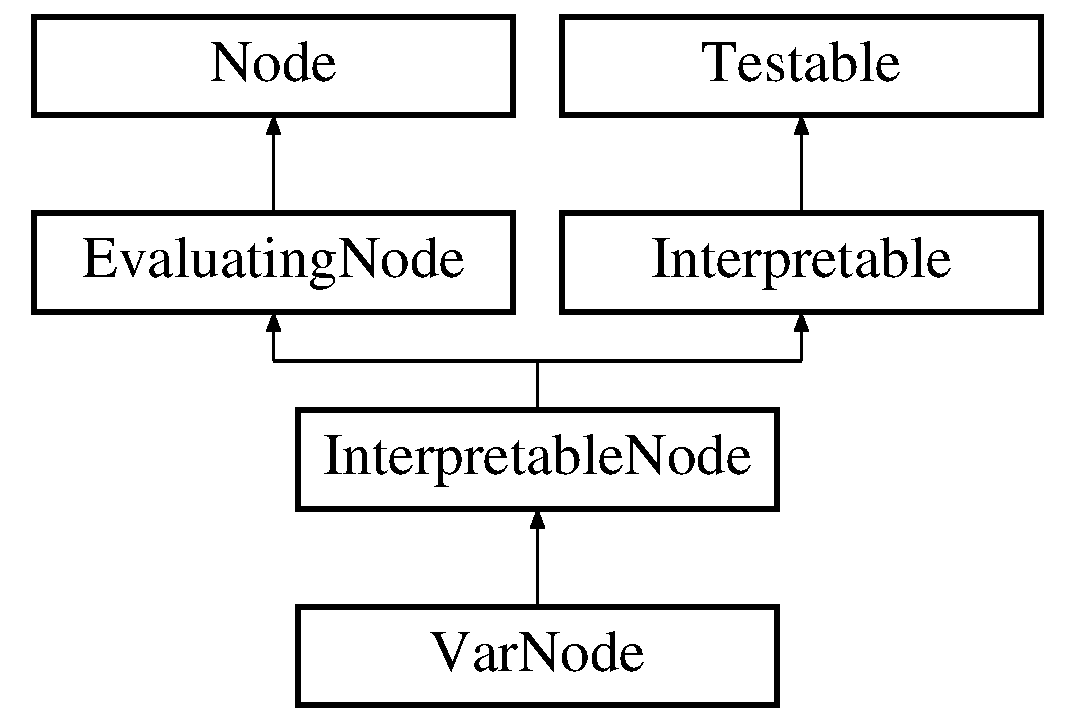
\includegraphics[height=4.000000cm]{classVarNode}
\end{center}
\end{figure}
\subsection*{Public Member Functions}
\begin{DoxyCompactItemize}
\item 
\hyperlink{classVarNode_a86b94143b89fc73a69cafb025415689f}{Var\+Node} ()
\item 
virtual \hyperlink{classVarNode_aab6e763704273c00cd756edbdd0b13df}{$\sim$\+Var\+Node} ()
\item 
virtual void \hyperlink{classVarNode_afaca674319775ae5e8a4fb0e5ec7b59f}{test} (\hyperlink{classValidator}{Validator} $\ast$validator)
\item 
virtual \hyperlink{classValue}{Value} \hyperlink{classVarNode_af2eed4fcade96d174c5b1f623b6bcdf6}{interpret} (\hyperlink{classInterpreter}{Interpreter} $\ast$interpreter)
\item 
virtual void \hyperlink{classVarNode_affe926e80803de0a83ce88f9a0d97db3}{evaluate\+\_\+impl} (\hyperlink{classSystemHandler}{System\+Handler} $\ast$handler, \hyperlink{statics_8h_a6664c451ca7787483a7981cc1de68dbb}{E\+V\+A\+L\+U\+A\+T\+I\+O\+N\+\_\+\+T\+Y\+PE} expected\+\_\+evaluation, struct \hyperlink{structEvaluation}{Evaluation} $\ast$evaluation)
\item 
std\+::string \hyperlink{classVarNode_afcde838758181438e89f8f91699c9d5b}{get\+Type\+As\+String} ()
\item 
bool \hyperlink{classVarNode_ab433d17cf3b2002756931a4f74cc200a}{is\+Array} ()
\item 
bool \hyperlink{classVarNode_a0a735a87c57b56a0fbcb87ef3dd36c3f}{is\+Primitive} ()
\item 
bool \hyperlink{classVarNode_ae0c6e834fe26f709f3e6bc859bc4384f}{is\+Object} ()
\end{DoxyCompactItemize}
\subsection*{Public Attributes}
\begin{DoxyCompactItemize}
\item 
\hyperlink{classEvaluatingNode}{Evaluating\+Node} $\ast$ \hyperlink{classVarNode_a8aff9f630482d9f8570dd9feb10849cd}{type}
\item 
std\+::string \hyperlink{classVarNode_adcfff85229e23fb0670fa3fc14b830e0}{name}
\item 
\hyperlink{classInterpretableNode}{Interpretable\+Node} $\ast$ \hyperlink{classVarNode_a58798cdece4226f1e0b844c8cbcd5146}{value}
\item 
\hyperlink{statics_8h_a0cbe4939ec6da73b52afbebd794d60ba}{M\+O\+D\+I\+F\+I\+E\+R\+\_\+\+A\+C\+C\+E\+SS} \hyperlink{classVarNode_a9d3115ee1b8fde5fe1b9484b57dba54a}{access}
\item 
int \hyperlink{classVarNode_a408a93fc558984318fb6fdad5cb36077}{dimensions}
\end{DoxyCompactItemize}
\subsection*{Additional Inherited Members}


\subsection{Constructor \& Destructor Documentation}
\mbox{\Hypertarget{classVarNode_a86b94143b89fc73a69cafb025415689f}\label{classVarNode_a86b94143b89fc73a69cafb025415689f}} 
\index{Var\+Node@{Var\+Node}!Var\+Node@{Var\+Node}}
\index{Var\+Node@{Var\+Node}!Var\+Node@{Var\+Node}}
\subsubsection{\texorpdfstring{Var\+Node()}{VarNode()}}
{\footnotesize\ttfamily Var\+Node\+::\+Var\+Node (\begin{DoxyParamCaption}{ }\end{DoxyParamCaption})}

\mbox{\Hypertarget{classVarNode_aab6e763704273c00cd756edbdd0b13df}\label{classVarNode_aab6e763704273c00cd756edbdd0b13df}} 
\index{Var\+Node@{Var\+Node}!````~Var\+Node@{$\sim$\+Var\+Node}}
\index{````~Var\+Node@{$\sim$\+Var\+Node}!Var\+Node@{Var\+Node}}
\subsubsection{\texorpdfstring{$\sim$\+Var\+Node()}{~VarNode()}}
{\footnotesize\ttfamily virtual Var\+Node\+::$\sim$\+Var\+Node (\begin{DoxyParamCaption}{ }\end{DoxyParamCaption})\hspace{0.3cm}{\ttfamily [virtual]}}



\subsection{Member Function Documentation}
\mbox{\Hypertarget{classVarNode_affe926e80803de0a83ce88f9a0d97db3}\label{classVarNode_affe926e80803de0a83ce88f9a0d97db3}} 
\index{Var\+Node@{Var\+Node}!evaluate\+\_\+impl@{evaluate\+\_\+impl}}
\index{evaluate\+\_\+impl@{evaluate\+\_\+impl}!Var\+Node@{Var\+Node}}
\subsubsection{\texorpdfstring{evaluate\+\_\+impl()}{evaluate\_impl()}}
{\footnotesize\ttfamily virtual void Var\+Node\+::evaluate\+\_\+impl (\begin{DoxyParamCaption}\item[{\hyperlink{classSystemHandler}{System\+Handler} $\ast$}]{handler,  }\item[{\hyperlink{statics_8h_a6664c451ca7787483a7981cc1de68dbb}{E\+V\+A\+L\+U\+A\+T\+I\+O\+N\+\_\+\+T\+Y\+PE}}]{expected\+\_\+evaluation,  }\item[{struct \hyperlink{structEvaluation}{Evaluation} $\ast$}]{evaluation }\end{DoxyParamCaption})\hspace{0.3cm}{\ttfamily [virtual]}}



Implements \hyperlink{classEvaluatingNode_a085fa06e0b46a93c814dc55cda0c1b26}{Evaluating\+Node}.

\mbox{\Hypertarget{classVarNode_afcde838758181438e89f8f91699c9d5b}\label{classVarNode_afcde838758181438e89f8f91699c9d5b}} 
\index{Var\+Node@{Var\+Node}!get\+Type\+As\+String@{get\+Type\+As\+String}}
\index{get\+Type\+As\+String@{get\+Type\+As\+String}!Var\+Node@{Var\+Node}}
\subsubsection{\texorpdfstring{get\+Type\+As\+String()}{getTypeAsString()}}
{\footnotesize\ttfamily std\+::string Var\+Node\+::get\+Type\+As\+String (\begin{DoxyParamCaption}{ }\end{DoxyParamCaption})}

\mbox{\Hypertarget{classVarNode_af2eed4fcade96d174c5b1f623b6bcdf6}\label{classVarNode_af2eed4fcade96d174c5b1f623b6bcdf6}} 
\index{Var\+Node@{Var\+Node}!interpret@{interpret}}
\index{interpret@{interpret}!Var\+Node@{Var\+Node}}
\subsubsection{\texorpdfstring{interpret()}{interpret()}}
{\footnotesize\ttfamily virtual \hyperlink{classValue}{Value} Var\+Node\+::interpret (\begin{DoxyParamCaption}\item[{\hyperlink{classInterpreter}{Interpreter} $\ast$}]{interpreter }\end{DoxyParamCaption})\hspace{0.3cm}{\ttfamily [virtual]}}



Implements \hyperlink{classInterpretableNode_a9a466e7d65c4b323d2b96b4ac8396cd7}{Interpretable\+Node}.

\mbox{\Hypertarget{classVarNode_ab433d17cf3b2002756931a4f74cc200a}\label{classVarNode_ab433d17cf3b2002756931a4f74cc200a}} 
\index{Var\+Node@{Var\+Node}!is\+Array@{is\+Array}}
\index{is\+Array@{is\+Array}!Var\+Node@{Var\+Node}}
\subsubsection{\texorpdfstring{is\+Array()}{isArray()}}
{\footnotesize\ttfamily bool Var\+Node\+::is\+Array (\begin{DoxyParamCaption}{ }\end{DoxyParamCaption})}

\mbox{\Hypertarget{classVarNode_ae0c6e834fe26f709f3e6bc859bc4384f}\label{classVarNode_ae0c6e834fe26f709f3e6bc859bc4384f}} 
\index{Var\+Node@{Var\+Node}!is\+Object@{is\+Object}}
\index{is\+Object@{is\+Object}!Var\+Node@{Var\+Node}}
\subsubsection{\texorpdfstring{is\+Object()}{isObject()}}
{\footnotesize\ttfamily bool Var\+Node\+::is\+Object (\begin{DoxyParamCaption}{ }\end{DoxyParamCaption})}

\mbox{\Hypertarget{classVarNode_a0a735a87c57b56a0fbcb87ef3dd36c3f}\label{classVarNode_a0a735a87c57b56a0fbcb87ef3dd36c3f}} 
\index{Var\+Node@{Var\+Node}!is\+Primitive@{is\+Primitive}}
\index{is\+Primitive@{is\+Primitive}!Var\+Node@{Var\+Node}}
\subsubsection{\texorpdfstring{is\+Primitive()}{isPrimitive()}}
{\footnotesize\ttfamily bool Var\+Node\+::is\+Primitive (\begin{DoxyParamCaption}{ }\end{DoxyParamCaption})}

\mbox{\Hypertarget{classVarNode_afaca674319775ae5e8a4fb0e5ec7b59f}\label{classVarNode_afaca674319775ae5e8a4fb0e5ec7b59f}} 
\index{Var\+Node@{Var\+Node}!test@{test}}
\index{test@{test}!Var\+Node@{Var\+Node}}
\subsubsection{\texorpdfstring{test()}{test()}}
{\footnotesize\ttfamily virtual void Var\+Node\+::test (\begin{DoxyParamCaption}\item[{\hyperlink{classValidator}{Validator} $\ast$}]{validator }\end{DoxyParamCaption})\hspace{0.3cm}{\ttfamily [virtual]}}



Reimplemented from \hyperlink{classInterpretable_a32f547aaf68dcbab993284d3257ab010}{Interpretable}.



\subsection{Member Data Documentation}
\mbox{\Hypertarget{classVarNode_a9d3115ee1b8fde5fe1b9484b57dba54a}\label{classVarNode_a9d3115ee1b8fde5fe1b9484b57dba54a}} 
\index{Var\+Node@{Var\+Node}!access@{access}}
\index{access@{access}!Var\+Node@{Var\+Node}}
\subsubsection{\texorpdfstring{access}{access}}
{\footnotesize\ttfamily \hyperlink{statics_8h_a0cbe4939ec6da73b52afbebd794d60ba}{M\+O\+D\+I\+F\+I\+E\+R\+\_\+\+A\+C\+C\+E\+SS} Var\+Node\+::access}

\mbox{\Hypertarget{classVarNode_a408a93fc558984318fb6fdad5cb36077}\label{classVarNode_a408a93fc558984318fb6fdad5cb36077}} 
\index{Var\+Node@{Var\+Node}!dimensions@{dimensions}}
\index{dimensions@{dimensions}!Var\+Node@{Var\+Node}}
\subsubsection{\texorpdfstring{dimensions}{dimensions}}
{\footnotesize\ttfamily int Var\+Node\+::dimensions}

\mbox{\Hypertarget{classVarNode_adcfff85229e23fb0670fa3fc14b830e0}\label{classVarNode_adcfff85229e23fb0670fa3fc14b830e0}} 
\index{Var\+Node@{Var\+Node}!name@{name}}
\index{name@{name}!Var\+Node@{Var\+Node}}
\subsubsection{\texorpdfstring{name}{name}}
{\footnotesize\ttfamily std\+::string Var\+Node\+::name}

\mbox{\Hypertarget{classVarNode_a8aff9f630482d9f8570dd9feb10849cd}\label{classVarNode_a8aff9f630482d9f8570dd9feb10849cd}} 
\index{Var\+Node@{Var\+Node}!type@{type}}
\index{type@{type}!Var\+Node@{Var\+Node}}
\subsubsection{\texorpdfstring{type}{type}}
{\footnotesize\ttfamily \hyperlink{classEvaluatingNode}{Evaluating\+Node}$\ast$ Var\+Node\+::type}

\mbox{\Hypertarget{classVarNode_a58798cdece4226f1e0b844c8cbcd5146}\label{classVarNode_a58798cdece4226f1e0b844c8cbcd5146}} 
\index{Var\+Node@{Var\+Node}!value@{value}}
\index{value@{value}!Var\+Node@{Var\+Node}}
\subsubsection{\texorpdfstring{value}{value}}
{\footnotesize\ttfamily \hyperlink{classInterpretableNode}{Interpretable\+Node}$\ast$ Var\+Node\+::value}



The documentation for this class was generated from the following file\+:\begin{DoxyCompactItemize}
\item 
include/\hyperlink{varnode_8h}{varnode.\+h}\end{DoxyCompactItemize}

\hypertarget{classVarType}{}\section{Var\+Type Class Reference}
\label{classVarType}\index{Var\+Type@{Var\+Type}}


{\ttfamily \#include $<$vartype.\+h$>$}

\subsection*{Public Member Functions}
\begin{DoxyCompactItemize}
\item 
\hyperlink{classVarType_adddd6258ae800047f968361615eff16b}{Var\+Type} ()
\item 
virtual \hyperlink{classVarType_af090ea0ac8270c1566c592bd9b3df2e6}{$\sim$\+Var\+Type} ()
\item 
bool \hyperlink{classVarType_a28323b657730e9b806f4b87af777de43}{operator==} (const \hyperlink{classVarType}{Var\+Type} \&other) const
\end{DoxyCompactItemize}
\subsection*{Static Public Member Functions}
\begin{DoxyCompactItemize}
\item 
static \hyperlink{classVarType}{Var\+Type} \hyperlink{classVarType_ae9fb7114144fc70d399962c25ea24b9c}{from\+String} (std\+::string \hyperlink{classVarType_adeb99cb6a17ce9cee53c165c912a333f}{value})
\end{DoxyCompactItemize}
\subsection*{Public Attributes}
\begin{DoxyCompactItemize}
\item 
\hyperlink{statics_8h_a4c85b3a98d55cc0252806c950379cce0}{V\+A\+R\+I\+A\+B\+L\+E\+\_\+\+T\+Y\+PE} \hyperlink{classVarType_ada5e661872d79bc92631a1ac384d459e}{type}
\item 
std\+::string \hyperlink{classVarType_adeb99cb6a17ce9cee53c165c912a333f}{value}
\end{DoxyCompactItemize}


\subsection{Constructor \& Destructor Documentation}
\mbox{\Hypertarget{classVarType_adddd6258ae800047f968361615eff16b}\label{classVarType_adddd6258ae800047f968361615eff16b}} 
\index{Var\+Type@{Var\+Type}!Var\+Type@{Var\+Type}}
\index{Var\+Type@{Var\+Type}!Var\+Type@{Var\+Type}}
\subsubsection{\texorpdfstring{Var\+Type()}{VarType()}}
{\footnotesize\ttfamily Var\+Type\+::\+Var\+Type (\begin{DoxyParamCaption}{ }\end{DoxyParamCaption})}

\mbox{\Hypertarget{classVarType_af090ea0ac8270c1566c592bd9b3df2e6}\label{classVarType_af090ea0ac8270c1566c592bd9b3df2e6}} 
\index{Var\+Type@{Var\+Type}!````~Var\+Type@{$\sim$\+Var\+Type}}
\index{````~Var\+Type@{$\sim$\+Var\+Type}!Var\+Type@{Var\+Type}}
\subsubsection{\texorpdfstring{$\sim$\+Var\+Type()}{~VarType()}}
{\footnotesize\ttfamily virtual Var\+Type\+::$\sim$\+Var\+Type (\begin{DoxyParamCaption}{ }\end{DoxyParamCaption})\hspace{0.3cm}{\ttfamily [virtual]}}



\subsection{Member Function Documentation}
\mbox{\Hypertarget{classVarType_ae9fb7114144fc70d399962c25ea24b9c}\label{classVarType_ae9fb7114144fc70d399962c25ea24b9c}} 
\index{Var\+Type@{Var\+Type}!from\+String@{from\+String}}
\index{from\+String@{from\+String}!Var\+Type@{Var\+Type}}
\subsubsection{\texorpdfstring{from\+String()}{fromString()}}
{\footnotesize\ttfamily static \hyperlink{classVarType}{Var\+Type} Var\+Type\+::from\+String (\begin{DoxyParamCaption}\item[{std\+::string}]{value }\end{DoxyParamCaption})\hspace{0.3cm}{\ttfamily [static]}}

\mbox{\Hypertarget{classVarType_a28323b657730e9b806f4b87af777de43}\label{classVarType_a28323b657730e9b806f4b87af777de43}} 
\index{Var\+Type@{Var\+Type}!operator==@{operator==}}
\index{operator==@{operator==}!Var\+Type@{Var\+Type}}
\subsubsection{\texorpdfstring{operator==()}{operator==()}}
{\footnotesize\ttfamily bool Var\+Type\+::operator== (\begin{DoxyParamCaption}\item[{const \hyperlink{classVarType}{Var\+Type} \&}]{other }\end{DoxyParamCaption}) const}



\subsection{Member Data Documentation}
\mbox{\Hypertarget{classVarType_ada5e661872d79bc92631a1ac384d459e}\label{classVarType_ada5e661872d79bc92631a1ac384d459e}} 
\index{Var\+Type@{Var\+Type}!type@{type}}
\index{type@{type}!Var\+Type@{Var\+Type}}
\subsubsection{\texorpdfstring{type}{type}}
{\footnotesize\ttfamily \hyperlink{statics_8h_a4c85b3a98d55cc0252806c950379cce0}{V\+A\+R\+I\+A\+B\+L\+E\+\_\+\+T\+Y\+PE} Var\+Type\+::type}

\mbox{\Hypertarget{classVarType_adeb99cb6a17ce9cee53c165c912a333f}\label{classVarType_adeb99cb6a17ce9cee53c165c912a333f}} 
\index{Var\+Type@{Var\+Type}!value@{value}}
\index{value@{value}!Var\+Type@{Var\+Type}}
\subsubsection{\texorpdfstring{value}{value}}
{\footnotesize\ttfamily std\+::string Var\+Type\+::value}



The documentation for this class was generated from the following file\+:\begin{DoxyCompactItemize}
\item 
include/\hyperlink{vartype_8h}{vartype.\+h}\end{DoxyCompactItemize}

\hypertarget{classWrittenFunction}{}\section{Written\+Function Class Reference}
\label{classWrittenFunction}\index{Written\+Function@{Written\+Function}}


{\ttfamily \#include $<$writtenfunction.\+h$>$}

Inheritance diagram for Written\+Function\+:\begin{figure}[H]
\begin{center}
\leavevmode
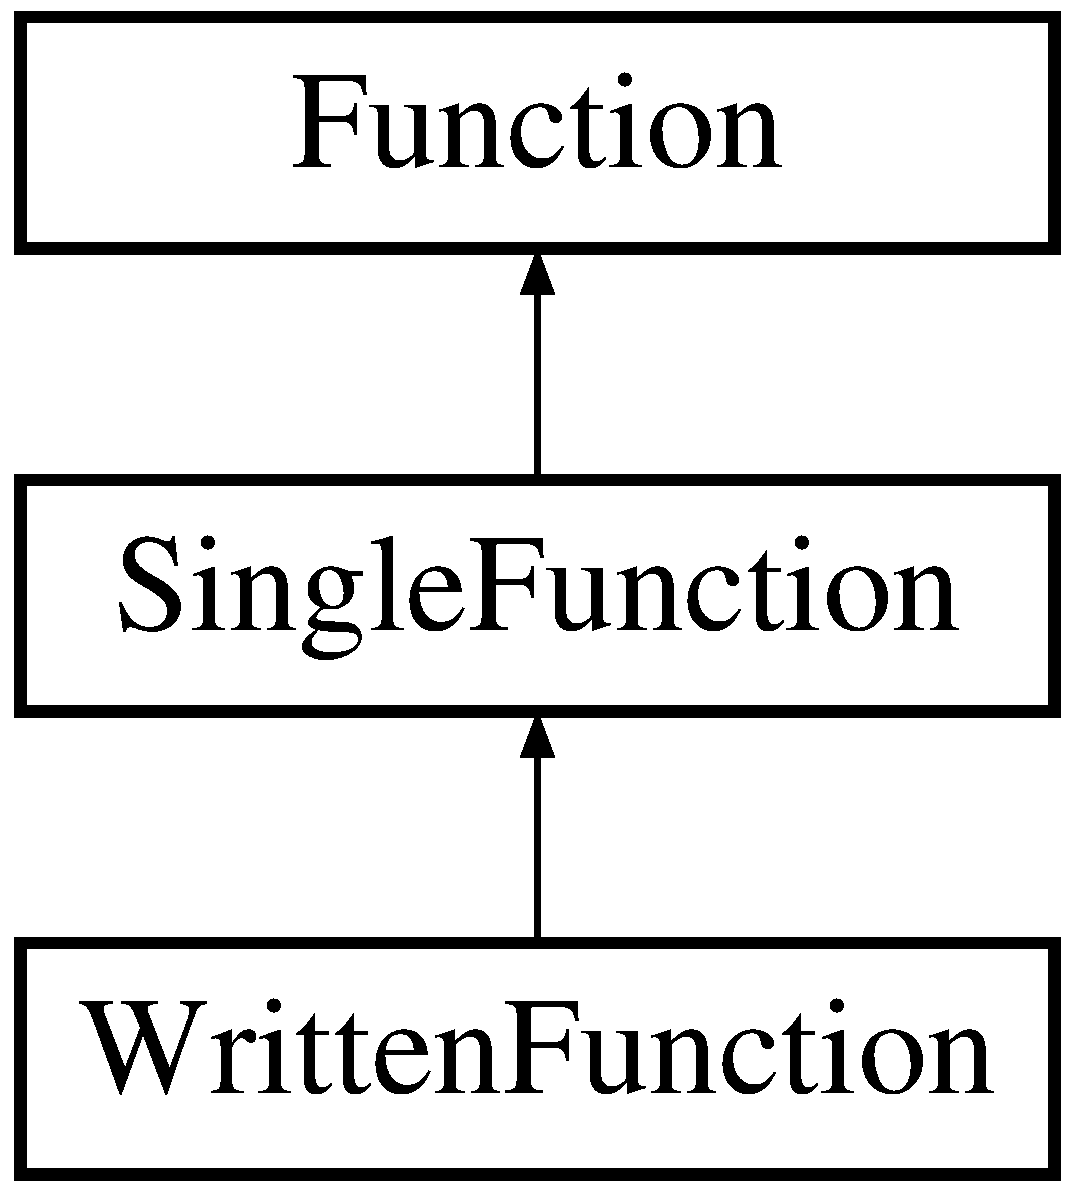
\includegraphics[height=2.000000cm]{classWrittenFunction}
\end{center}
\end{figure}
\subsection*{Public Member Functions}
\begin{DoxyCompactItemize}
\item 
\hyperlink{classWrittenFunction_a5bdf425b86c5dbfd481a2d265a889c88}{Written\+Function} (\hyperlink{classInterpreter}{Interpreter} $\ast$interpreter, \hyperlink{classFunctionNode}{Function\+Node} $\ast$function\+\_\+node)
\item 
virtual \hyperlink{classWrittenFunction_a46facc10f998146c7709772b0b662ad6}{$\sim$\+Written\+Function} ()
\item 
virtual void \hyperlink{classWrittenFunction_afe56e5eb6a13f6e38ab5ec87e371d745}{invoke} (std\+::vector$<$ \hyperlink{classValue}{Value} $>$ values, \hyperlink{classValue}{Value} $\ast$return\+\_\+value, std\+::shared\+\_\+ptr$<$ \hyperlink{classObject}{Object} $>$ object)
\end{DoxyCompactItemize}
\subsection*{Additional Inherited Members}


\subsection{Constructor \& Destructor Documentation}
\mbox{\Hypertarget{classWrittenFunction_a5bdf425b86c5dbfd481a2d265a889c88}\label{classWrittenFunction_a5bdf425b86c5dbfd481a2d265a889c88}} 
\index{Written\+Function@{Written\+Function}!Written\+Function@{Written\+Function}}
\index{Written\+Function@{Written\+Function}!Written\+Function@{Written\+Function}}
\subsubsection{\texorpdfstring{Written\+Function()}{WrittenFunction()}}
{\footnotesize\ttfamily Written\+Function\+::\+Written\+Function (\begin{DoxyParamCaption}\item[{\hyperlink{classInterpreter}{Interpreter} $\ast$}]{interpreter,  }\item[{\hyperlink{classFunctionNode}{Function\+Node} $\ast$}]{function\+\_\+node }\end{DoxyParamCaption})}

\mbox{\Hypertarget{classWrittenFunction_a46facc10f998146c7709772b0b662ad6}\label{classWrittenFunction_a46facc10f998146c7709772b0b662ad6}} 
\index{Written\+Function@{Written\+Function}!````~Written\+Function@{$\sim$\+Written\+Function}}
\index{````~Written\+Function@{$\sim$\+Written\+Function}!Written\+Function@{Written\+Function}}
\subsubsection{\texorpdfstring{$\sim$\+Written\+Function()}{~WrittenFunction()}}
{\footnotesize\ttfamily virtual Written\+Function\+::$\sim$\+Written\+Function (\begin{DoxyParamCaption}{ }\end{DoxyParamCaption})\hspace{0.3cm}{\ttfamily [virtual]}}



\subsection{Member Function Documentation}
\mbox{\Hypertarget{classWrittenFunction_afe56e5eb6a13f6e38ab5ec87e371d745}\label{classWrittenFunction_afe56e5eb6a13f6e38ab5ec87e371d745}} 
\index{Written\+Function@{Written\+Function}!invoke@{invoke}}
\index{invoke@{invoke}!Written\+Function@{Written\+Function}}
\subsubsection{\texorpdfstring{invoke()}{invoke()}}
{\footnotesize\ttfamily virtual void Written\+Function\+::invoke (\begin{DoxyParamCaption}\item[{std\+::vector$<$ \hyperlink{classValue}{Value} $>$}]{values,  }\item[{\hyperlink{classValue}{Value} $\ast$}]{return\+\_\+value,  }\item[{std\+::shared\+\_\+ptr$<$ \hyperlink{classObject}{Object} $>$}]{object }\end{DoxyParamCaption})\hspace{0.3cm}{\ttfamily [virtual]}}



Implements \hyperlink{classFunction_a84f9a63e68becc27e58ea738ba4cd698}{Function}.



The documentation for this class was generated from the following file\+:\begin{DoxyCompactItemize}
\item 
include/\hyperlink{writtenfunction_8h}{writtenfunction.\+h}\end{DoxyCompactItemize}

\chapter{File Documentation}
\hypertarget{array_8h}{}\section{include/array.h File Reference}
\label{array_8h}\index{include/array.\+h@{include/array.\+h}}
{\ttfamily \#include \char`\"{}object.\+h\char`\"{}}\newline
\subsection*{Classes}
\begin{DoxyCompactItemize}
\item 
class \hyperlink{classArray}{Array}
\end{DoxyCompactItemize}

\hypertarget{arraynode_8h}{}\section{include/arraynode.h File Reference}
\label{arraynode_8h}\index{include/arraynode.\+h@{include/arraynode.\+h}}
{\ttfamily \#include \char`\"{}einode.\+h\char`\"{}}\newline
\subsection*{Classes}
\begin{DoxyCompactItemize}
\item 
class \hyperlink{classArrayNode}{Array\+Node}
\end{DoxyCompactItemize}

\hypertarget{bodynode_8h}{}\section{include/bodynode.h File Reference}
\label{bodynode_8h}\index{include/bodynode.\+h@{include/bodynode.\+h}}
{\ttfamily \#include $<$vector$>$}\newline
{\ttfamily \#include $<$functional$>$}\newline
{\ttfamily \#include \char`\"{}inode.\+h\char`\"{}}\newline
\subsection*{Classes}
\begin{DoxyCompactItemize}
\item 
class \hyperlink{classBodyNode}{Body\+Node}
\end{DoxyCompactItemize}

\hypertarget{castnode_8h}{}\section{include/castnode.h File Reference}
\label{castnode_8h}\index{include/castnode.\+h@{include/castnode.\+h}}
{\ttfamily \#include \char`\"{}einode.\+h\char`\"{}}\newline
\subsection*{Classes}
\begin{DoxyCompactItemize}
\item 
class \hyperlink{classCastNode}{Cast\+Node}
\end{DoxyCompactItemize}

\hypertarget{class_8h}{}\section{include/class.h File Reference}
\label{class_8h}\index{include/class.\+h@{include/class.\+h}}
{\ttfamily \#include $<$string$>$}\newline
{\ttfamily \#include $<$vector$>$}\newline
{\ttfamily \#include \char`\"{}variable.\+h\char`\"{}}\newline
{\ttfamily \#include \char`\"{}functionsystem.\+h\char`\"{}}\newline
\subsection*{Classes}
\begin{DoxyCompactItemize}
\item 
class \hyperlink{classClass}{Class}
\end{DoxyCompactItemize}

\hypertarget{classnode_8h}{}\section{include/classnode.h File Reference}
\label{classnode_8h}\index{include/classnode.\+h@{include/classnode.\+h}}
{\ttfamily \#include $<$iostream$>$}\newline
{\ttfamily \#include \char`\"{}inode.\+h\char`\"{}}\newline
\subsection*{Classes}
\begin{DoxyCompactItemize}
\item 
class \hyperlink{classClassNode}{Class\+Node}
\end{DoxyCompactItemize}

\hypertarget{config_8h}{}\section{include/config.h File Reference}
\label{config_8h}\index{include/config.\+h@{include/config.\+h}}
\subsection*{Macros}
\begin{DoxyCompactItemize}
\item 
\#define \hyperlink{config_8h_ab74ab2d1d7cf7cd1bbffaf7c1e076700}{M\+A\+X\+\_\+\+K\+E\+Y\+W\+O\+R\+D\+\_\+\+S\+I\+ZE}~10
\item 
\#define \hyperlink{config_8h_a742adcc33a031116a6d08af3aea2e07a}{M\+A\+X\+\_\+\+O\+P\+E\+R\+A\+T\+O\+R\+S\+\_\+\+S\+I\+ZE}~3
\item 
\#define \hyperlink{config_8h_a7d2ae674cad5299a52b0e7dceac10087}{D\+E\+B\+U\+G\+\_\+\+E\+N\+A\+B\+L\+ED}
\end{DoxyCompactItemize}


\subsection{Macro Definition Documentation}
\mbox{\Hypertarget{config_8h_a7d2ae674cad5299a52b0e7dceac10087}\label{config_8h_a7d2ae674cad5299a52b0e7dceac10087}} 
\index{config.\+h@{config.\+h}!D\+E\+B\+U\+G\+\_\+\+E\+N\+A\+B\+L\+ED@{D\+E\+B\+U\+G\+\_\+\+E\+N\+A\+B\+L\+ED}}
\index{D\+E\+B\+U\+G\+\_\+\+E\+N\+A\+B\+L\+ED@{D\+E\+B\+U\+G\+\_\+\+E\+N\+A\+B\+L\+ED}!config.\+h@{config.\+h}}
\subsubsection{\texorpdfstring{D\+E\+B\+U\+G\+\_\+\+E\+N\+A\+B\+L\+ED}{DEBUG\_ENABLED}}
{\footnotesize\ttfamily \#define D\+E\+B\+U\+G\+\_\+\+E\+N\+A\+B\+L\+ED}

\mbox{\Hypertarget{config_8h_ab74ab2d1d7cf7cd1bbffaf7c1e076700}\label{config_8h_ab74ab2d1d7cf7cd1bbffaf7c1e076700}} 
\index{config.\+h@{config.\+h}!M\+A\+X\+\_\+\+K\+E\+Y\+W\+O\+R\+D\+\_\+\+S\+I\+ZE@{M\+A\+X\+\_\+\+K\+E\+Y\+W\+O\+R\+D\+\_\+\+S\+I\+ZE}}
\index{M\+A\+X\+\_\+\+K\+E\+Y\+W\+O\+R\+D\+\_\+\+S\+I\+ZE@{M\+A\+X\+\_\+\+K\+E\+Y\+W\+O\+R\+D\+\_\+\+S\+I\+ZE}!config.\+h@{config.\+h}}
\subsubsection{\texorpdfstring{M\+A\+X\+\_\+\+K\+E\+Y\+W\+O\+R\+D\+\_\+\+S\+I\+ZE}{MAX\_KEYWORD\_SIZE}}
{\footnotesize\ttfamily \#define M\+A\+X\+\_\+\+K\+E\+Y\+W\+O\+R\+D\+\_\+\+S\+I\+ZE~10}

\mbox{\Hypertarget{config_8h_a742adcc33a031116a6d08af3aea2e07a}\label{config_8h_a742adcc33a031116a6d08af3aea2e07a}} 
\index{config.\+h@{config.\+h}!M\+A\+X\+\_\+\+O\+P\+E\+R\+A\+T\+O\+R\+S\+\_\+\+S\+I\+ZE@{M\+A\+X\+\_\+\+O\+P\+E\+R\+A\+T\+O\+R\+S\+\_\+\+S\+I\+ZE}}
\index{M\+A\+X\+\_\+\+O\+P\+E\+R\+A\+T\+O\+R\+S\+\_\+\+S\+I\+ZE@{M\+A\+X\+\_\+\+O\+P\+E\+R\+A\+T\+O\+R\+S\+\_\+\+S\+I\+ZE}!config.\+h@{config.\+h}}
\subsubsection{\texorpdfstring{M\+A\+X\+\_\+\+O\+P\+E\+R\+A\+T\+O\+R\+S\+\_\+\+S\+I\+ZE}{MAX\_OPERATORS\_SIZE}}
{\footnotesize\ttfamily \#define M\+A\+X\+\_\+\+O\+P\+E\+R\+A\+T\+O\+R\+S\+\_\+\+S\+I\+ZE~3}


\hypertarget{cpointers_8h}{}\section{include/cpointers.h File Reference}
\label{cpointers_8h}\index{include/cpointers.\+h@{include/cpointers.\+h}}
{\ttfamily \#include $<$memory$>$}\newline
{\ttfamily \#include $<$iostream$>$}\newline
{\ttfamily \#include $<$vector$>$}\newline
\subsection*{Classes}
\begin{DoxyCompactItemize}
\item 
class \hyperlink{classSharedSelfHoldingPointer}{Shared\+Self\+Holding\+Pointer$<$ T $>$}
\item 
class \hyperlink{classSharedSelfHoldingPointer}{Shared\+Self\+Holding\+Pointer$<$ T $>$}
\end{DoxyCompactItemize}

\hypertarget{csystem_8h}{}\section{include/csystem.h File Reference}
\label{csystem_8h}\index{include/csystem.\+h@{include/csystem.\+h}}
{\ttfamily \#include $<$vector$>$}\newline
{\ttfamily \#include $<$memory$>$}\newline
{\ttfamily \#include \char`\"{}class.\+h\char`\"{}}\newline
\subsection*{Classes}
\begin{DoxyCompactItemize}
\item 
class \hyperlink{classClassSystem}{Class\+System}
\end{DoxyCompactItemize}

\hypertarget{datatype_8h}{}\section{include/datatype.h File Reference}
\label{datatype_8h}\index{include/datatype.\+h@{include/datatype.\+h}}
{\ttfamily \#include $<$string$>$}\newline
\subsection*{Classes}
\begin{DoxyCompactItemize}
\item 
class \hyperlink{classDataType}{Data\+Type}
\end{DoxyCompactItemize}

\hypertarget{debug_8h}{}\section{include/debug.h File Reference}
\label{debug_8h}\index{include/debug.\+h@{include/debug.\+h}}
{\ttfamily \#include \char`\"{}config.\+h\char`\"{}}\newline
{\ttfamily \#include $<$memory$>$}\newline
{\ttfamily \#include \char`\"{}node.\+h\char`\"{}}\newline
\subsection*{Classes}
\begin{DoxyCompactItemize}
\item 
class \hyperlink{classDebug}{Debug}
\end{DoxyCompactItemize}

\hypertarget{einode_8h}{}\section{include/einode.h File Reference}
\label{einode_8h}\index{include/einode.\+h@{include/einode.\+h}}
{\ttfamily \#include \char`\"{}inode.\+h\char`\"{}}\newline
\subsection*{Classes}
\begin{DoxyCompactItemize}
\item 
class \hyperlink{classExpressionInterpretableNode}{Expression\+Interpretable\+Node}
\end{DoxyCompactItemize}

\hypertarget{evaluatingnode_8h}{}\section{include/evaluatingnode.h File Reference}
\label{evaluatingnode_8h}\index{include/evaluatingnode.\+h@{include/evaluatingnode.\+h}}
{\ttfamily \#include \char`\"{}node.\+h\char`\"{}}\newline
{\ttfamily \#include \char`\"{}statics.\+h\char`\"{}}\newline
\subsection*{Classes}
\begin{DoxyCompactItemize}
\item 
struct \hyperlink{structEvaluation}{Evaluation}
\item 
struct \hyperlink{structEvaluation_1_1datatype}{Evaluation\+::datatype}
\item 
class \hyperlink{classEvaluatingNode}{Evaluating\+Node}
\end{DoxyCompactItemize}

\hypertarget{expnode_8h}{}\section{include/expnode.h File Reference}
\label{expnode_8h}\index{include/expnode.\+h@{include/expnode.\+h}}
{\ttfamily \#include $<$memory$>$}\newline
{\ttfamily \#include \char`\"{}statics.\+h\char`\"{}}\newline
{\ttfamily \#include \char`\"{}einode.\+h\char`\"{}}\newline
{\ttfamily \#include \char`\"{}evaluatingnode.\+h\char`\"{}}\newline
{\ttfamily \#include \char`\"{}validator.\+h\char`\"{}}\newline
\subsection*{Classes}
\begin{DoxyCompactItemize}
\item 
class \hyperlink{classExpNode}{Exp\+Node}
\end{DoxyCompactItemize}

\hypertarget{fcnode_8h}{}\section{include/fcnode.h File Reference}
\label{fcnode_8h}\index{include/fcnode.\+h@{include/fcnode.\+h}}
{\ttfamily \#include \char`\"{}node.\+h\char`\"{}}\newline
{\ttfamily \#include \char`\"{}einode.\+h\char`\"{}}\newline
{\ttfamily \#include \char`\"{}value.\+h\char`\"{}}\newline
{\ttfamily \#include $<$vector$>$}\newline
\subsection*{Classes}
\begin{DoxyCompactItemize}
\item 
class \hyperlink{classFunctionCallNode}{Function\+Call\+Node}
\end{DoxyCompactItemize}

\hypertarget{fnode_8h}{}\section{include/fnode.h File Reference}
\label{fnode_8h}\index{include/fnode.\+h@{include/fnode.\+h}}
{\ttfamily \#include \char`\"{}einode.\+h\char`\"{}}\newline
{\ttfamily \#include $<$string$>$}\newline
{\ttfamily \#include $<$vector$>$}\newline
\subsection*{Classes}
\begin{DoxyCompactItemize}
\item 
class \hyperlink{classFunctionNode}{Function\+Node}
\end{DoxyCompactItemize}

\hypertarget{function_8h}{}\section{include/function.h File Reference}
\label{function_8h}\index{include/function.\+h@{include/function.\+h}}
{\ttfamily \#include $<$vector$>$}\newline
{\ttfamily \#include $<$memory$>$}\newline
{\ttfamily \#include \char`\"{}value.\+h\char`\"{}}\newline
{\ttfamily \#include \char`\"{}object.\+h\char`\"{}}\newline
\subsection*{Classes}
\begin{DoxyCompactItemize}
\item 
class \hyperlink{classFunction}{Function}
\end{DoxyCompactItemize}

\hypertarget{functionsystem_8h}{}\section{include/functionsystem.h File Reference}
\label{functionsystem_8h}\index{include/functionsystem.\+h@{include/functionsystem.\+h}}
{\ttfamily \#include $<$functional$>$}\newline
{\ttfamily \#include $<$memory$>$}\newline
{\ttfamily \#include $<$vector$>$}\newline
{\ttfamily \#include $<$stdexcept$>$}\newline
{\ttfamily \#include \char`\"{}value.\+h\char`\"{}}\newline
\subsection*{Classes}
\begin{DoxyCompactItemize}
\item 
class \hyperlink{classFunctionSystem}{Function\+System}
\end{DoxyCompactItemize}

\hypertarget{groupedfunction_8h}{}\section{include/groupedfunction.h File Reference}
\label{groupedfunction_8h}\index{include/groupedfunction.\+h@{include/groupedfunction.\+h}}
{\ttfamily \#include \char`\"{}function.\+h\char`\"{}}\newline
\subsection*{Classes}
\begin{DoxyCompactItemize}
\item 
class \hyperlink{classGroupedFunction}{Grouped\+Function}
\end{DoxyCompactItemize}

\hypertarget{identifiernode_8h}{}\section{include/identifiernode.h File Reference}
\label{identifiernode_8h}\index{include/identifiernode.\+h@{include/identifiernode.\+h}}
{\ttfamily \#include \char`\"{}einode.\+h\char`\"{}}\newline
{\ttfamily \#include \char`\"{}statics.\+h\char`\"{}}\newline
{\ttfamily \#include $<$string$>$}\newline
\subsection*{Classes}
\begin{DoxyCompactItemize}
\item 
class \hyperlink{classIdentifierNode}{Identifier\+Node}
\end{DoxyCompactItemize}

\hypertarget{ifstmtnode_8h}{}\section{include/ifstmtnode.h File Reference}
\label{ifstmtnode_8h}\index{include/ifstmtnode.\+h@{include/ifstmtnode.\+h}}
{\ttfamily \#include \char`\"{}statement.\+h\char`\"{}}\newline
{\ttfamily \#include \char`\"{}einode.\+h\char`\"{}}\newline
\subsection*{Classes}
\begin{DoxyCompactItemize}
\item 
class \hyperlink{classIfStatementNode}{If\+Statement\+Node}
\end{DoxyCompactItemize}

\hypertarget{inode_8h}{}\section{include/inode.h File Reference}
\label{inode_8h}\index{include/inode.\+h@{include/inode.\+h}}
{\ttfamily \#include \char`\"{}evaluatingnode.\+h\char`\"{}}\newline
{\ttfamily \#include \char`\"{}interpretable.\+h\char`\"{}}\newline
\subsection*{Classes}
\begin{DoxyCompactItemize}
\item 
class \hyperlink{classInterpretableNode}{Interpretable\+Node}
\end{DoxyCompactItemize}

\hypertarget{interpretable_8h}{}\section{include/interpretable.h File Reference}
\label{interpretable_8h}\index{include/interpretable.\+h@{include/interpretable.\+h}}
{\ttfamily \#include \char`\"{}statics.\+h\char`\"{}}\newline
{\ttfamily \#include \char`\"{}value.\+h\char`\"{}}\newline
{\ttfamily \#include \char`\"{}testable.\+h\char`\"{}}\newline
{\ttfamily \#include $<$iostream$>$}\newline
\subsection*{Classes}
\begin{DoxyCompactItemize}
\item 
class \hyperlink{classInterpretable}{Interpretable}
\end{DoxyCompactItemize}

\hypertarget{interpreter_8h}{}\section{include/interpreter.h File Reference}
\label{interpreter_8h}\index{include/interpreter.\+h@{include/interpreter.\+h}}
{\ttfamily \#include $<$string.\+h$>$}\newline
{\ttfamily \#include $<$memory$>$}\newline
{\ttfamily \#include $<$vector$>$}\newline
{\ttfamily \#include \char`\"{}scope.\+h\char`\"{}}\newline
{\ttfamily \#include \char`\"{}functionsystem.\+h\char`\"{}}\newline
{\ttfamily \#include \char`\"{}csystem.\+h\char`\"{}}\newline
{\ttfamily \#include \char`\"{}systemhandler.\+h\char`\"{}}\newline
{\ttfamily \#include \char`\"{}logger.\+h\char`\"{}}\newline
\subsection*{Classes}
\begin{DoxyCompactItemize}
\item 
class \hyperlink{classInterpreter}{Interpreter}
\end{DoxyCompactItemize}
\subsection*{Typedefs}
\begin{DoxyCompactItemize}
\item 
typedef std\+::function$<$ void(const char $\ast$output)$>$ \hyperlink{interpreter_8h_a57e80eaa218fd4f66b1d55c833119967}{O\+U\+T\+P\+U\+T\+\_\+\+F\+U\+N\+C\+T\+I\+ON}
\end{DoxyCompactItemize}


\subsection{Typedef Documentation}
\mbox{\Hypertarget{interpreter_8h_a57e80eaa218fd4f66b1d55c833119967}\label{interpreter_8h_a57e80eaa218fd4f66b1d55c833119967}} 
\index{interpreter.\+h@{interpreter.\+h}!O\+U\+T\+P\+U\+T\+\_\+\+F\+U\+N\+C\+T\+I\+ON@{O\+U\+T\+P\+U\+T\+\_\+\+F\+U\+N\+C\+T\+I\+ON}}
\index{O\+U\+T\+P\+U\+T\+\_\+\+F\+U\+N\+C\+T\+I\+ON@{O\+U\+T\+P\+U\+T\+\_\+\+F\+U\+N\+C\+T\+I\+ON}!interpreter.\+h@{interpreter.\+h}}
\subsubsection{\texorpdfstring{O\+U\+T\+P\+U\+T\+\_\+\+F\+U\+N\+C\+T\+I\+ON}{OUTPUT\_FUNCTION}}
{\footnotesize\ttfamily typedef std\+::function$<$void(const char$\ast$ output)$>$ \hyperlink{interpreter_8h_a57e80eaa218fd4f66b1d55c833119967}{O\+U\+T\+P\+U\+T\+\_\+\+F\+U\+N\+C\+T\+I\+ON}}


\hypertarget{keywordnode_8h}{}\section{include/keywordnode.h File Reference}
\label{keywordnode_8h}\index{include/keywordnode.\+h@{include/keywordnode.\+h}}
{\ttfamily \#include \char`\"{}evaluatingnode.\+h\char`\"{}}\newline
{\ttfamily \#include $<$string$>$}\newline
\subsection*{Classes}
\begin{DoxyCompactItemize}
\item 
class \hyperlink{classKeywordNode}{Keyword\+Node}
\end{DoxyCompactItemize}

\hypertarget{lexer_8h}{}\section{include/lexer.h File Reference}
\label{lexer_8h}\index{include/lexer.\+h@{include/lexer.\+h}}
{\ttfamily \#include $<$vector$>$}\newline
{\ttfamily \#include $<$memory$>$}\newline
{\ttfamily \#include \char`\"{}tokenfactory.\+h\char`\"{}}\newline
{\ttfamily \#include \char`\"{}token.\+h\char`\"{}}\newline
{\ttfamily \#include \char`\"{}logger.\+h\char`\"{}}\newline
\subsection*{Classes}
\begin{DoxyCompactItemize}
\item 
class \hyperlink{classLexer}{Lexer}
\end{DoxyCompactItemize}

\hypertarget{literalnode_8h}{}\section{include/literalnode.h File Reference}
\label{literalnode_8h}\index{include/literalnode.\+h@{include/literalnode.\+h}}
{\ttfamily \#include \char`\"{}einode.\+h\char`\"{}}\newline
\subsection*{Classes}
\begin{DoxyCompactItemize}
\item 
class \hyperlink{classLiteralNode}{Literal\+Node}
\end{DoxyCompactItemize}

\hypertarget{logger_8h}{}\section{include/logger.h File Reference}
\label{logger_8h}\index{include/logger.\+h@{include/logger.\+h}}
{\ttfamily \#include \char`\"{}statics.\+h\char`\"{}}\newline
{\ttfamily \#include $<$string$>$}\newline
{\ttfamily \#include $<$vector$>$}\newline
{\ttfamily \#include \char`\"{}posinfo.\+h\char`\"{}}\newline
\subsection*{Classes}
\begin{DoxyCompactItemize}
\item 
class \hyperlink{classLogEntry}{Log\+Entry}
\item 
class \hyperlink{classLogger}{Logger}
\end{DoxyCompactItemize}

\hypertarget{nativefunction_8h}{}\section{include/nativefunction.h File Reference}
\label{nativefunction_8h}\index{include/nativefunction.\+h@{include/nativefunction.\+h}}
{\ttfamily \#include \char`\"{}singlefunction.\+h\char`\"{}}\newline
\subsection*{Classes}
\begin{DoxyCompactItemize}
\item 
class \hyperlink{classNativeFunction}{Native\+Function}
\end{DoxyCompactItemize}

\hypertarget{negnode_8h}{}\section{include/negnode.h File Reference}
\label{negnode_8h}\index{include/negnode.\+h@{include/negnode.\+h}}
{\ttfamily \#include \char`\"{}einode.\+h\char`\"{}}\newline
\subsection*{Classes}
\begin{DoxyCompactItemize}
\item 
class \hyperlink{classNegNode}{Neg\+Node}
\end{DoxyCompactItemize}

\hypertarget{newnode_8h}{}\section{include/newnode.h File Reference}
\label{newnode_8h}\index{include/newnode.\+h@{include/newnode.\+h}}
{\ttfamily \#include \char`\"{}einode.\+h\char`\"{}}\newline
{\ttfamily \#include $<$vector$>$}\newline
\subsection*{Classes}
\begin{DoxyCompactItemize}
\item 
class \hyperlink{classNewNode}{New\+Node}
\end{DoxyCompactItemize}

\hypertarget{node_8h}{}\section{include/node.h File Reference}
\label{node_8h}\index{include/node.\+h@{include/node.\+h}}
{\ttfamily \#include $<$memory$>$}\newline
{\ttfamily \#include \char`\"{}posinfo.\+h\char`\"{}}\newline
\subsection*{Classes}
\begin{DoxyCompactItemize}
\item 
class \hyperlink{classNode}{Node}
\end{DoxyCompactItemize}

\hypertarget{nodefactory_8h}{}\section{include/nodefactory.h File Reference}
\label{nodefactory_8h}\index{include/nodefactory.\+h@{include/nodefactory.\+h}}
{\ttfamily \#include $<$memory$>$}\newline
{\ttfamily \#include $<$vector$>$}\newline
{\ttfamily \#include \char`\"{}statics.\+h\char`\"{}}\newline
{\ttfamily \#include \char`\"{}posinfo.\+h\char`\"{}}\newline
\subsection*{Classes}
\begin{DoxyCompactItemize}
\item 
class \hyperlink{classNodeFactory}{Node\+Factory}
\end{DoxyCompactItemize}

\hypertarget{nodes_8h}{}\section{include/nodes.h File Reference}
\label{nodes_8h}\index{include/nodes.\+h@{include/nodes.\+h}}
{\ttfamily \#include \char`\"{}node.\+h\char`\"{}}\newline
{\ttfamily \#include \char`\"{}expnode.\+h\char`\"{}}\newline
{\ttfamily \#include \char`\"{}varnode.\+h\char`\"{}}\newline
{\ttfamily \#include \char`\"{}literalnode.\+h\char`\"{}}\newline
{\ttfamily \#include \char`\"{}identifiernode.\+h\char`\"{}}\newline
{\ttfamily \#include \char`\"{}stringnode.\+h\char`\"{}}\newline
{\ttfamily \#include \char`\"{}keywordnode.\+h\char`\"{}}\newline
{\ttfamily \#include \char`\"{}fcnode.\+h\char`\"{}}\newline
{\ttfamily \#include \char`\"{}negnode.\+h\char`\"{}}\newline
{\ttfamily \#include \char`\"{}ifstmtnode.\+h\char`\"{}}\newline
{\ttfamily \#include \char`\"{}bodynode.\+h\char`\"{}}\newline
{\ttfamily \#include \char`\"{}castnode.\+h\char`\"{}}\newline
{\ttfamily \#include \char`\"{}arraynode.\+h\char`\"{}}\newline
{\ttfamily \#include \char`\"{}newnode.\+h\char`\"{}}\newline
{\ttfamily \#include \char`\"{}fnode.\+h\char`\"{}}\newline
{\ttfamily \#include \char`\"{}inode.\+h\char`\"{}}\newline
{\ttfamily \#include \char`\"{}einode.\+h\char`\"{}}\newline
{\ttfamily \#include \char`\"{}retnode.\+h\char`\"{}}\newline
{\ttfamily \#include \char`\"{}classnode.\+h\char`\"{}}\newline
{\ttfamily \#include \char`\"{}evaluatingnode.\+h\char`\"{}}\newline

\hypertarget{object_8h}{}\section{include/object.h File Reference}
\label{object_8h}\index{include/object.\+h@{include/object.\+h}}
{\ttfamily \#include $<$memory$>$}\newline
{\ttfamily \#include \char`\"{}class.\+h\char`\"{}}\newline
{\ttfamily \#include \char`\"{}scope.\+h\char`\"{}}\newline
\subsection*{Classes}
\begin{DoxyCompactItemize}
\item 
class \hyperlink{classObject}{Object}
\end{DoxyCompactItemize}

\hypertarget{parser_8h}{}\section{include/parser.h File Reference}
\label{parser_8h}\index{include/parser.\+h@{include/parser.\+h}}
{\ttfamily \#include $<$vector$>$}\newline
{\ttfamily \#include $<$string$>$}\newline
{\ttfamily \#include $<$memory$>$}\newline
{\ttfamily \#include \char`\"{}nodes.\+h\char`\"{}}\newline
{\ttfamily \#include \char`\"{}statics.\+h\char`\"{}}\newline
{\ttfamily \#include \char`\"{}token.\+h\char`\"{}}\newline
{\ttfamily \#include \char`\"{}nodefactory.\+h\char`\"{}}\newline
{\ttfamily \#include \char`\"{}logger.\+h\char`\"{}}\newline
\subsection*{Classes}
\begin{DoxyCompactItemize}
\item 
struct \hyperlink{structorder__of__operation}{order\+\_\+of\+\_\+operation}
\item 
class \hyperlink{classParser}{Parser}
\end{DoxyCompactItemize}

\hypertarget{posinfo_8h}{}\section{include/posinfo.h File Reference}
\label{posinfo_8h}\index{include/posinfo.\+h@{include/posinfo.\+h}}
\subsection*{Classes}
\begin{DoxyCompactItemize}
\item 
class \hyperlink{classPosInfo}{Pos\+Info}
\end{DoxyCompactItemize}

\hypertarget{retnode_8h}{}\section{include/retnode.h File Reference}
\label{retnode_8h}\index{include/retnode.\+h@{include/retnode.\+h}}
{\ttfamily \#include \char`\"{}inode.\+h\char`\"{}}\newline
\subsection*{Classes}
\begin{DoxyCompactItemize}
\item 
class \hyperlink{classReturnNode}{Return\+Node}
\end{DoxyCompactItemize}

\hypertarget{scope_8h}{}\section{include/scope.h File Reference}
\label{scope_8h}\index{include/scope.\+h@{include/scope.\+h}}
{\ttfamily \#include $<$memory$>$}\newline
{\ttfamily \#include $<$vector$>$}\newline
{\ttfamily \#include $<$string$>$}\newline
{\ttfamily \#include \char`\"{}variable.\+h\char`\"{}}\newline
\subsection*{Classes}
\begin{DoxyCompactItemize}
\item 
class \hyperlink{classScope}{Scope}
\end{DoxyCompactItemize}

\hypertarget{scopehandler_8h}{}\section{include/scopehandler.h File Reference}
\label{scopehandler_8h}\index{include/scopehandler.\+h@{include/scopehandler.\+h}}
{\ttfamily \#include \char`\"{}scope.\+h\char`\"{}}\newline
\subsection*{Classes}
\begin{DoxyCompactItemize}
\item 
class \hyperlink{classScopeHandler}{Scope\+Handler}
\end{DoxyCompactItemize}

\hypertarget{singlefunction_8h}{}\section{include/singlefunction.h File Reference}
\label{singlefunction_8h}\index{include/singlefunction.\+h@{include/singlefunction.\+h}}
{\ttfamily \#include $<$vector$>$}\newline
{\ttfamily \#include $<$memory$>$}\newline
{\ttfamily \#include \char`\"{}value.\+h\char`\"{}}\newline
{\ttfamily \#include \char`\"{}object.\+h\char`\"{}}\newline
{\ttfamily \#include \char`\"{}vartype.\+h\char`\"{}}\newline
{\ttfamily \#include \char`\"{}function.\+h\char`\"{}}\newline
\subsection*{Classes}
\begin{DoxyCompactItemize}
\item 
class \hyperlink{classSingleFunction}{Single\+Function}
\end{DoxyCompactItemize}

\hypertarget{splitter_8h}{}\section{include/splitter.h File Reference}
\label{splitter_8h}\index{include/splitter.\+h@{include/splitter.\+h}}
{\ttfamily \#include $<$iostream$>$}\newline
\subsection*{Classes}
\begin{DoxyCompactItemize}
\item 
struct \hyperlink{structdata__descriptor}{data\+\_\+descriptor}
\item 
struct \hyperlink{structoutput__data}{output\+\_\+data}
\item 
struct \hyperlink{structmarble__code}{marble\+\_\+code}
\item 
struct \hyperlink{structsplit}{split}
\item 
class \hyperlink{classSplitter}{Splitter}
\end{DoxyCompactItemize}

\hypertarget{statement_8h}{}\section{include/statement.h File Reference}
\label{statement_8h}\index{include/statement.\+h@{include/statement.\+h}}
{\ttfamily \#include \char`\"{}node.\+h\char`\"{}}\newline
{\ttfamily \#include \char`\"{}inode.\+h\char`\"{}}\newline
{\ttfamily \#include \char`\"{}bodynode.\+h\char`\"{}}\newline
\subsection*{Classes}
\begin{DoxyCompactItemize}
\item 
class \hyperlink{classStatement}{Statement}
\end{DoxyCompactItemize}

\hypertarget{statics_8h}{}\section{include/statics.h File Reference}
\label{statics_8h}\index{include/statics.\+h@{include/statics.\+h}}
\subsection*{Typedefs}
\begin{DoxyCompactItemize}
\item 
typedef int \hyperlink{statics_8h_a28f867553077bc713fdf8921a9226e2e}{S\+Y\+S\+T\+E\+M\+\_\+\+H\+A\+N\+D\+L\+E\+R\+\_\+\+T\+Y\+PE}
\item 
typedef int \hyperlink{statics_8h_adb8e9416fa8b5ea4961e9f171db14133}{T\+O\+K\+E\+N\+\_\+\+T\+Y\+PE}
\item 
typedef int \hyperlink{statics_8h_a1ec6d4bfce2e004debbc141eafc512db}{N\+O\+D\+E\+\_\+\+T\+Y\+PE}
\item 
typedef int \hyperlink{statics_8h_a0674a913b8e8c8a9f265baab3646b565}{V\+A\+L\+U\+E\+\_\+\+T\+Y\+PE}
\item 
typedef int \hyperlink{statics_8h_a4c85b3a98d55cc0252806c950379cce0}{V\+A\+R\+I\+A\+B\+L\+E\+\_\+\+T\+Y\+PE}
\item 
typedef int \hyperlink{statics_8h_a6664c451ca7787483a7981cc1de68dbb}{E\+V\+A\+L\+U\+A\+T\+I\+O\+N\+\_\+\+T\+Y\+PE}
\item 
typedef int \hyperlink{statics_8h_a025d9866e39f51183a23b3e2165f0e77}{F\+U\+N\+C\+T\+I\+O\+N\+\_\+\+T\+Y\+PE}
\item 
typedef int \hyperlink{statics_8h_a4cb76ced721b70f0ecadc88b0ac66518}{L\+O\+G\+\_\+\+T\+Y\+PE}
\item 
typedef int \hyperlink{statics_8h_a0cbe4939ec6da73b52afbebd794d60ba}{M\+O\+D\+I\+F\+I\+E\+R\+\_\+\+A\+C\+C\+E\+SS}
\end{DoxyCompactItemize}
\subsection*{Enumerations}
\begin{DoxyCompactItemize}
\item 
enum \{ \hyperlink{statics_8h_a06fc87d81c62e9abb8790b6e5713c55ba26f155f830094369c46c8c5351aa766d}{S\+Y\+S\+T\+E\+M\+\_\+\+H\+A\+N\+D\+L\+E\+R\+\_\+\+V\+A\+L\+I\+D\+A\+T\+OR}, 
\hyperlink{statics_8h_a06fc87d81c62e9abb8790b6e5713c55ba8120abce982a5d0f7a5cd2b2daffa32a}{S\+Y\+S\+T\+E\+M\+\_\+\+H\+A\+N\+D\+L\+E\+R\+\_\+\+I\+N\+T\+E\+R\+P\+R\+E\+T\+ER}
 \}
\item 
enum \{ \newline
\hyperlink{statics_8h_adf764cbdea00d65edcd07bb9953ad2b7a35478580250fd6b1fd85ae9af496e032}{T\+O\+K\+E\+N\+\_\+\+T\+Y\+P\+E\+\_\+\+N\+U\+M\+B\+ER}, 
\hyperlink{statics_8h_adf764cbdea00d65edcd07bb9953ad2b7aa0616d64220313ebe455b14194772387}{T\+O\+K\+E\+N\+\_\+\+T\+Y\+P\+E\+\_\+\+O\+P\+E\+R\+A\+T\+OR}, 
\hyperlink{statics_8h_adf764cbdea00d65edcd07bb9953ad2b7ad3cf9bb5db6cbbb7ad327eccf69ed183}{T\+O\+K\+E\+N\+\_\+\+T\+Y\+P\+E\+\_\+\+S\+T\+R\+I\+NG}, 
\hyperlink{statics_8h_adf764cbdea00d65edcd07bb9953ad2b7ab9a8e35e5b5128713fc7520bc48c311d}{T\+O\+K\+E\+N\+\_\+\+T\+Y\+P\+E\+\_\+\+I\+D\+E\+N\+T\+I\+F\+I\+ER}, 
\newline
\hyperlink{statics_8h_adf764cbdea00d65edcd07bb9953ad2b7a5c27ab4f822d8a9d3ad48daa86c05fe3}{T\+O\+K\+E\+N\+\_\+\+T\+Y\+P\+E\+\_\+\+K\+E\+Y\+W\+O\+RD}, 
\hyperlink{statics_8h_adf764cbdea00d65edcd07bb9953ad2b7a0a45e1337367457ddc1579ae79b1a737}{T\+O\+K\+E\+N\+\_\+\+T\+Y\+P\+E\+\_\+\+S\+Y\+M\+B\+OL}
 \}
\item 
enum \{ \newline
\hyperlink{statics_8h_a99fb83031ce9923c84392b4e92f956b5a33eeb39261e1ec1d8aa030bdda180874}{N\+O\+D\+E\+\_\+\+T\+Y\+P\+E\+\_\+\+V\+A\+R\+I\+A\+B\+L\+E\+\_\+\+D\+E\+C\+L\+A\+R\+A\+T\+I\+ON}, 
\hyperlink{statics_8h_a99fb83031ce9923c84392b4e92f956b5a2d0ba5e1136613275698aa8e4096c5f9}{N\+O\+D\+E\+\_\+\+T\+Y\+P\+E\+\_\+\+E\+X\+P\+R\+E\+S\+S\+I\+ON}, 
\hyperlink{statics_8h_a99fb83031ce9923c84392b4e92f956b5a65faa6ad96887e847d758ebef480fa6c}{N\+O\+D\+E\+\_\+\+T\+Y\+P\+E\+\_\+\+L\+I\+T\+E\+R\+AL}, 
\hyperlink{statics_8h_a99fb83031ce9923c84392b4e92f956b5a087591f7e60eaa9d1d4f5ef9e22a57d3}{N\+O\+D\+E\+\_\+\+T\+Y\+P\+E\+\_\+\+I\+D\+E\+N\+T\+I\+F\+I\+ER}, 
\newline
\hyperlink{statics_8h_a99fb83031ce9923c84392b4e92f956b5a99a5a0f5142b463e9dc9c2dcd5804500}{N\+O\+D\+E\+\_\+\+T\+Y\+P\+E\+\_\+\+S\+T\+R\+I\+NG}, 
\hyperlink{statics_8h_a99fb83031ce9923c84392b4e92f956b5a2d82baa755064e4ce6fea2c879f042e8}{N\+O\+D\+E\+\_\+\+T\+Y\+P\+E\+\_\+\+K\+E\+Y\+W\+O\+RD}, 
\hyperlink{statics_8h_a99fb83031ce9923c84392b4e92f956b5a2676df9b727837a4cad511b7e211f221}{N\+O\+D\+E\+\_\+\+T\+Y\+P\+E\+\_\+\+F\+U\+N\+C\+T\+I\+O\+N\+\_\+\+C\+A\+LL}, 
\hyperlink{statics_8h_a99fb83031ce9923c84392b4e92f956b5a0f50ca170413904a279fbe1b179fc348}{N\+O\+D\+E\+\_\+\+T\+Y\+P\+E\+\_\+\+N\+E\+G\+A\+T\+I\+VE}, 
\newline
\hyperlink{statics_8h_a99fb83031ce9923c84392b4e92f956b5aa1780beac4cd9e52c764d3c5cb029edb}{N\+O\+D\+E\+\_\+\+T\+Y\+P\+E\+\_\+\+I\+F\+\_\+\+S\+T\+MT}, 
\hyperlink{statics_8h_a99fb83031ce9923c84392b4e92f956b5a3fe0bc832a83348710eec9224d6e1a95}{N\+O\+D\+E\+\_\+\+T\+Y\+P\+E\+\_\+\+B\+O\+DY}, 
\hyperlink{statics_8h_a99fb83031ce9923c84392b4e92f956b5ac6f9926fda81a85e995bd00fac7cfc34}{N\+O\+D\+E\+\_\+\+T\+Y\+P\+E\+\_\+\+C\+A\+ST}, 
\hyperlink{statics_8h_a99fb83031ce9923c84392b4e92f956b5aea6c674c869c495f6a70f5cc7f112f64}{N\+O\+D\+E\+\_\+\+T\+Y\+P\+E\+\_\+\+A\+R\+R\+AY}, 
\newline
\hyperlink{statics_8h_a99fb83031ce9923c84392b4e92f956b5a6b7e7fbdf0127397a99a49e433e9b8b8}{N\+O\+D\+E\+\_\+\+T\+Y\+P\+E\+\_\+\+N\+EW}, 
\hyperlink{statics_8h_a99fb83031ce9923c84392b4e92f956b5aa0722b3a089966fb2121f42a294e4b4d}{N\+O\+D\+E\+\_\+\+T\+Y\+P\+E\+\_\+\+F\+U\+N\+C\+T\+I\+ON}, 
\hyperlink{statics_8h_a99fb83031ce9923c84392b4e92f956b5aec1a1538fc11354beb3d9d5f79349728}{N\+O\+D\+E\+\_\+\+T\+Y\+P\+E\+\_\+\+R\+E\+T\+U\+RN}, 
\hyperlink{statics_8h_a99fb83031ce9923c84392b4e92f956b5a8bc0966c42f92af1ee1a0a44a596ee9f}{N\+O\+D\+E\+\_\+\+T\+Y\+P\+E\+\_\+\+C\+L\+A\+SS}
 \}
\item 
enum \{ \hyperlink{statics_8h_abc6126af1d45847bc59afa0aa3216b04a40ce59abb6734fd8b6f49c298d1cfc10}{F\+U\+N\+C\+T\+I\+O\+N\+\_\+\+T\+Y\+P\+E\+\_\+\+W\+R\+I\+T\+T\+EN}, 
\hyperlink{statics_8h_abc6126af1d45847bc59afa0aa3216b04a092cdfecc53fef53ad5143a23c07b2ce}{F\+U\+N\+C\+T\+I\+O\+N\+\_\+\+T\+Y\+P\+E\+\_\+\+N\+A\+T\+I\+VE}, 
\hyperlink{statics_8h_abc6126af1d45847bc59afa0aa3216b04a2a89bbf4fa7f79000044aa22ca7c7d99}{F\+U\+N\+C\+T\+I\+O\+N\+\_\+\+T\+Y\+P\+E\+\_\+\+G\+R\+O\+U\+P\+ED}
 \}
\item 
enum \{ \newline
\hyperlink{statics_8h_adc29c2ff13d900c2f185ee95427fb06caf2ee83e2357d49573892b7ae397d80b1}{V\+A\+R\+I\+A\+B\+L\+E\+\_\+\+T\+Y\+P\+E\+\_\+\+N\+U\+M\+B\+ER}, 
\hyperlink{statics_8h_adc29c2ff13d900c2f185ee95427fb06ca43b1a6f7095cfebb0ed1e291863c77e5}{V\+A\+R\+I\+A\+B\+L\+E\+\_\+\+T\+Y\+P\+E\+\_\+\+S\+T\+R\+I\+NG}, 
\hyperlink{statics_8h_adc29c2ff13d900c2f185ee95427fb06ca3e4a14b07951247d02a1805e4852c772}{V\+A\+R\+I\+A\+B\+L\+E\+\_\+\+T\+Y\+P\+E\+\_\+\+O\+B\+J\+E\+CT}, 
\hyperlink{statics_8h_adc29c2ff13d900c2f185ee95427fb06ca7c00101b597a357b429d235f334d791a}{V\+A\+R\+I\+A\+B\+L\+E\+\_\+\+T\+Y\+P\+E\+\_\+\+A\+R\+R\+AY}, 
\newline
\hyperlink{statics_8h_adc29c2ff13d900c2f185ee95427fb06ca323361ec76d177b874d670f08b17588d}{V\+A\+R\+I\+A\+B\+L\+E\+\_\+\+T\+Y\+P\+E\+\_\+\+B\+Y\+TE}, 
\hyperlink{statics_8h_adc29c2ff13d900c2f185ee95427fb06caadedea18e71b62139fa249d9528fa405}{V\+A\+R\+I\+A\+B\+L\+E\+\_\+\+T\+Y\+P\+E\+\_\+\+V\+O\+ID}
 \}
\item 
enum \{ \newline
\hyperlink{statics_8h_a61dadd085c1777f559549e05962b2c9ea6041458fe9d34323ca7ce1db2bf4cf3f}{V\+A\+L\+U\+E\+\_\+\+T\+Y\+P\+E\+\_\+\+N\+U\+M\+B\+ER}, 
\hyperlink{statics_8h_a61dadd085c1777f559549e05962b2c9eab03274454ef6b98f8fe4f002cfe97f7c}{V\+A\+L\+U\+E\+\_\+\+T\+Y\+P\+E\+\_\+\+S\+T\+R\+I\+NG}, 
\hyperlink{statics_8h_a61dadd085c1777f559549e05962b2c9eaf9a03ab49b38e79e4fe9571ba7a90624}{V\+A\+L\+U\+E\+\_\+\+T\+Y\+P\+E\+\_\+\+O\+B\+J\+E\+CT}, 
\hyperlink{statics_8h_a61dadd085c1777f559549e05962b2c9ea0b448f3dba11aee279a32513e01bf3ad}{V\+A\+L\+U\+E\+\_\+\+T\+Y\+P\+E\+\_\+\+A\+R\+R\+AY}, 
\newline
\hyperlink{statics_8h_a61dadd085c1777f559549e05962b2c9ea93391cf7e956d706b81a1892f0aaa79c}{V\+A\+L\+U\+E\+\_\+\+T\+Y\+P\+E\+\_\+\+B\+Y\+TE}
 \}
\item 
enum \{ \hyperlink{statics_8h_a726ca809ffd3d67ab4b8476646f26635aafe78609d5ada883f93962938d055b2e}{E\+V\+A\+L\+U\+A\+T\+I\+O\+N\+\_\+\+T\+Y\+P\+E\+\_\+\+D\+A\+T\+A\+T\+Y\+PE} = 0x01, 
\hyperlink{statics_8h_a726ca809ffd3d67ab4b8476646f26635a6cf684a91ca9fa5ca311c6a36531cb64}{E\+V\+A\+L\+U\+A\+T\+I\+O\+N\+\_\+\+T\+Y\+P\+E\+\_\+\+V\+A\+R\+I\+A\+B\+LE} = 0x02, 
\hyperlink{statics_8h_a726ca809ffd3d67ab4b8476646f26635a2ab06a574bf346e4e69dcd93d3769a13}{E\+V\+A\+L\+U\+A\+T\+I\+O\+N\+\_\+\+F\+R\+O\+M\+\_\+\+V\+A\+R\+I\+A\+B\+LE} = 0x04
 \}
\item 
enum \{ \hyperlink{statics_8h_a0411cd49bb5b71852cecd93bcbf0ca2da2586b14dd32a915699420f30e573ef21}{M\+O\+D\+I\+F\+I\+E\+R\+\_\+\+A\+C\+C\+E\+S\+S\+\_\+\+P\+R\+I\+V\+A\+TE}, 
\hyperlink{statics_8h_a0411cd49bb5b71852cecd93bcbf0ca2da33fa49b8342a45277313f2606132a385}{M\+O\+D\+I\+F\+I\+E\+R\+\_\+\+A\+C\+C\+E\+S\+S\+\_\+\+P\+R\+O\+T\+E\+C\+T\+ED}, 
\hyperlink{statics_8h_a0411cd49bb5b71852cecd93bcbf0ca2daa5eb5cc604ee3951758da828bf828e9c}{M\+O\+D\+I\+F\+I\+E\+R\+\_\+\+A\+C\+C\+E\+S\+S\+\_\+\+P\+U\+B\+L\+IC}
 \}
\item 
enum \{ \hyperlink{statics_8h_abed82baf7f470b522273a3e37c24c600a55b57dce74f14a62104ae66e62789eb3}{L\+E\+F\+T\+\_\+\+T\+O\+\_\+\+R\+I\+G\+HT}, 
\hyperlink{statics_8h_abed82baf7f470b522273a3e37c24c600a054986f32cd1cb5ade35758f8947c42c}{R\+I\+G\+H\+T\+\_\+\+T\+O\+\_\+\+L\+E\+FT}, 
\hyperlink{statics_8h_abed82baf7f470b522273a3e37c24c600af92dc91effb86ddcb411e2f6dc2d1b5c}{N\+O\+N\+\_\+\+A\+S\+S\+O\+C\+I\+A\+T\+I\+VE}
 \}
\item 
enum \{ \newline
\hyperlink{statics_8h_ab04a0655cd1e3bcac5e8f48c18df1a57ae938817999785609d14713432ebd62d9}{I\+S\+\_\+\+C\+H\+A\+R\+A\+C\+T\+ER}, 
\hyperlink{statics_8h_ab04a0655cd1e3bcac5e8f48c18df1a57a9adf1295d4d18abf5cc6dca100778c81}{I\+S\+\_\+\+N\+U\+M\+B\+ER}, 
\hyperlink{statics_8h_ab04a0655cd1e3bcac5e8f48c18df1a57ab12c6b4d3577f5aa2dcf015e8470c2c4}{I\+S\+\_\+\+O\+P\+E\+R\+A\+T\+OR}, 
\hyperlink{statics_8h_ab04a0655cd1e3bcac5e8f48c18df1a57a4e0bcfd74cff01de3bbfef6d50cfd349}{I\+S\+\_\+\+S\+Y\+M\+B\+OL}, 
\newline
\hyperlink{statics_8h_ab04a0655cd1e3bcac5e8f48c18df1a57a5d056468bbac07e125cb8982b44b31bd}{I\+S\+\_\+\+W\+H\+I\+T\+E\+S\+P\+A\+CE}
 \}
\item 
enum \{ \hyperlink{statics_8h_a385c44f6fb256e5716a2302a5b940388a031c67cea5434164f0e8c5e9f3fb9de8}{R\+U\+L\+E\+\_\+\+P\+A\+R\+S\+E\+\_\+\+C\+A\+S\+T\+I\+NG} = 0x01, 
\hyperlink{statics_8h_a385c44f6fb256e5716a2302a5b940388abe138e46b8b7f932885978c3f27f2109}{R\+U\+L\+E\+\_\+\+P\+A\+R\+S\+E\+\_\+\+A\+R\+R\+AY} = 0x02
 \}
\item 
enum \{ \hyperlink{statics_8h_abc5c98fcc1211af2b80116dd6e0a035da23ae4d711a7bbb3900240cb7316b4b4e}{L\+O\+G\+\_\+\+L\+E\+V\+E\+L\+\_\+\+N\+O\+T\+I\+CE}, 
\hyperlink{statics_8h_abc5c98fcc1211af2b80116dd6e0a035da5b4dd81b4dc7eefbc55ba03415c627ef}{L\+O\+G\+\_\+\+L\+E\+V\+E\+L\+\_\+\+W\+A\+R\+N\+I\+NG}, 
\hyperlink{statics_8h_abc5c98fcc1211af2b80116dd6e0a035da5b40f003febbc3b535649d63f4b8a44f}{L\+O\+G\+\_\+\+L\+E\+V\+E\+L\+\_\+\+E\+R\+R\+OR}
 \}
\end{DoxyCompactItemize}


\subsection{Typedef Documentation}
\mbox{\Hypertarget{statics_8h_a6664c451ca7787483a7981cc1de68dbb}\label{statics_8h_a6664c451ca7787483a7981cc1de68dbb}} 
\index{statics.\+h@{statics.\+h}!E\+V\+A\+L\+U\+A\+T\+I\+O\+N\+\_\+\+T\+Y\+PE@{E\+V\+A\+L\+U\+A\+T\+I\+O\+N\+\_\+\+T\+Y\+PE}}
\index{E\+V\+A\+L\+U\+A\+T\+I\+O\+N\+\_\+\+T\+Y\+PE@{E\+V\+A\+L\+U\+A\+T\+I\+O\+N\+\_\+\+T\+Y\+PE}!statics.\+h@{statics.\+h}}
\subsubsection{\texorpdfstring{E\+V\+A\+L\+U\+A\+T\+I\+O\+N\+\_\+\+T\+Y\+PE}{EVALUATION\_TYPE}}
{\footnotesize\ttfamily typedef int \hyperlink{statics_8h_a6664c451ca7787483a7981cc1de68dbb}{E\+V\+A\+L\+U\+A\+T\+I\+O\+N\+\_\+\+T\+Y\+PE}}

\mbox{\Hypertarget{statics_8h_a025d9866e39f51183a23b3e2165f0e77}\label{statics_8h_a025d9866e39f51183a23b3e2165f0e77}} 
\index{statics.\+h@{statics.\+h}!F\+U\+N\+C\+T\+I\+O\+N\+\_\+\+T\+Y\+PE@{F\+U\+N\+C\+T\+I\+O\+N\+\_\+\+T\+Y\+PE}}
\index{F\+U\+N\+C\+T\+I\+O\+N\+\_\+\+T\+Y\+PE@{F\+U\+N\+C\+T\+I\+O\+N\+\_\+\+T\+Y\+PE}!statics.\+h@{statics.\+h}}
\subsubsection{\texorpdfstring{F\+U\+N\+C\+T\+I\+O\+N\+\_\+\+T\+Y\+PE}{FUNCTION\_TYPE}}
{\footnotesize\ttfamily typedef int \hyperlink{statics_8h_a025d9866e39f51183a23b3e2165f0e77}{F\+U\+N\+C\+T\+I\+O\+N\+\_\+\+T\+Y\+PE}}

\mbox{\Hypertarget{statics_8h_a4cb76ced721b70f0ecadc88b0ac66518}\label{statics_8h_a4cb76ced721b70f0ecadc88b0ac66518}} 
\index{statics.\+h@{statics.\+h}!L\+O\+G\+\_\+\+T\+Y\+PE@{L\+O\+G\+\_\+\+T\+Y\+PE}}
\index{L\+O\+G\+\_\+\+T\+Y\+PE@{L\+O\+G\+\_\+\+T\+Y\+PE}!statics.\+h@{statics.\+h}}
\subsubsection{\texorpdfstring{L\+O\+G\+\_\+\+T\+Y\+PE}{LOG\_TYPE}}
{\footnotesize\ttfamily typedef int \hyperlink{statics_8h_a4cb76ced721b70f0ecadc88b0ac66518}{L\+O\+G\+\_\+\+T\+Y\+PE}}

\mbox{\Hypertarget{statics_8h_a0cbe4939ec6da73b52afbebd794d60ba}\label{statics_8h_a0cbe4939ec6da73b52afbebd794d60ba}} 
\index{statics.\+h@{statics.\+h}!M\+O\+D\+I\+F\+I\+E\+R\+\_\+\+A\+C\+C\+E\+SS@{M\+O\+D\+I\+F\+I\+E\+R\+\_\+\+A\+C\+C\+E\+SS}}
\index{M\+O\+D\+I\+F\+I\+E\+R\+\_\+\+A\+C\+C\+E\+SS@{M\+O\+D\+I\+F\+I\+E\+R\+\_\+\+A\+C\+C\+E\+SS}!statics.\+h@{statics.\+h}}
\subsubsection{\texorpdfstring{M\+O\+D\+I\+F\+I\+E\+R\+\_\+\+A\+C\+C\+E\+SS}{MODIFIER\_ACCESS}}
{\footnotesize\ttfamily typedef int \hyperlink{statics_8h_a0cbe4939ec6da73b52afbebd794d60ba}{M\+O\+D\+I\+F\+I\+E\+R\+\_\+\+A\+C\+C\+E\+SS}}

\mbox{\Hypertarget{statics_8h_a1ec6d4bfce2e004debbc141eafc512db}\label{statics_8h_a1ec6d4bfce2e004debbc141eafc512db}} 
\index{statics.\+h@{statics.\+h}!N\+O\+D\+E\+\_\+\+T\+Y\+PE@{N\+O\+D\+E\+\_\+\+T\+Y\+PE}}
\index{N\+O\+D\+E\+\_\+\+T\+Y\+PE@{N\+O\+D\+E\+\_\+\+T\+Y\+PE}!statics.\+h@{statics.\+h}}
\subsubsection{\texorpdfstring{N\+O\+D\+E\+\_\+\+T\+Y\+PE}{NODE\_TYPE}}
{\footnotesize\ttfamily typedef int \hyperlink{statics_8h_a1ec6d4bfce2e004debbc141eafc512db}{N\+O\+D\+E\+\_\+\+T\+Y\+PE}}

\mbox{\Hypertarget{statics_8h_a28f867553077bc713fdf8921a9226e2e}\label{statics_8h_a28f867553077bc713fdf8921a9226e2e}} 
\index{statics.\+h@{statics.\+h}!S\+Y\+S\+T\+E\+M\+\_\+\+H\+A\+N\+D\+L\+E\+R\+\_\+\+T\+Y\+PE@{S\+Y\+S\+T\+E\+M\+\_\+\+H\+A\+N\+D\+L\+E\+R\+\_\+\+T\+Y\+PE}}
\index{S\+Y\+S\+T\+E\+M\+\_\+\+H\+A\+N\+D\+L\+E\+R\+\_\+\+T\+Y\+PE@{S\+Y\+S\+T\+E\+M\+\_\+\+H\+A\+N\+D\+L\+E\+R\+\_\+\+T\+Y\+PE}!statics.\+h@{statics.\+h}}
\subsubsection{\texorpdfstring{S\+Y\+S\+T\+E\+M\+\_\+\+H\+A\+N\+D\+L\+E\+R\+\_\+\+T\+Y\+PE}{SYSTEM\_HANDLER\_TYPE}}
{\footnotesize\ttfamily typedef int \hyperlink{statics_8h_a28f867553077bc713fdf8921a9226e2e}{S\+Y\+S\+T\+E\+M\+\_\+\+H\+A\+N\+D\+L\+E\+R\+\_\+\+T\+Y\+PE}}

\mbox{\Hypertarget{statics_8h_adb8e9416fa8b5ea4961e9f171db14133}\label{statics_8h_adb8e9416fa8b5ea4961e9f171db14133}} 
\index{statics.\+h@{statics.\+h}!T\+O\+K\+E\+N\+\_\+\+T\+Y\+PE@{T\+O\+K\+E\+N\+\_\+\+T\+Y\+PE}}
\index{T\+O\+K\+E\+N\+\_\+\+T\+Y\+PE@{T\+O\+K\+E\+N\+\_\+\+T\+Y\+PE}!statics.\+h@{statics.\+h}}
\subsubsection{\texorpdfstring{T\+O\+K\+E\+N\+\_\+\+T\+Y\+PE}{TOKEN\_TYPE}}
{\footnotesize\ttfamily typedef int \hyperlink{statics_8h_adb8e9416fa8b5ea4961e9f171db14133}{T\+O\+K\+E\+N\+\_\+\+T\+Y\+PE}}

\mbox{\Hypertarget{statics_8h_a0674a913b8e8c8a9f265baab3646b565}\label{statics_8h_a0674a913b8e8c8a9f265baab3646b565}} 
\index{statics.\+h@{statics.\+h}!V\+A\+L\+U\+E\+\_\+\+T\+Y\+PE@{V\+A\+L\+U\+E\+\_\+\+T\+Y\+PE}}
\index{V\+A\+L\+U\+E\+\_\+\+T\+Y\+PE@{V\+A\+L\+U\+E\+\_\+\+T\+Y\+PE}!statics.\+h@{statics.\+h}}
\subsubsection{\texorpdfstring{V\+A\+L\+U\+E\+\_\+\+T\+Y\+PE}{VALUE\_TYPE}}
{\footnotesize\ttfamily typedef int \hyperlink{statics_8h_a0674a913b8e8c8a9f265baab3646b565}{V\+A\+L\+U\+E\+\_\+\+T\+Y\+PE}}

\mbox{\Hypertarget{statics_8h_a4c85b3a98d55cc0252806c950379cce0}\label{statics_8h_a4c85b3a98d55cc0252806c950379cce0}} 
\index{statics.\+h@{statics.\+h}!V\+A\+R\+I\+A\+B\+L\+E\+\_\+\+T\+Y\+PE@{V\+A\+R\+I\+A\+B\+L\+E\+\_\+\+T\+Y\+PE}}
\index{V\+A\+R\+I\+A\+B\+L\+E\+\_\+\+T\+Y\+PE@{V\+A\+R\+I\+A\+B\+L\+E\+\_\+\+T\+Y\+PE}!statics.\+h@{statics.\+h}}
\subsubsection{\texorpdfstring{V\+A\+R\+I\+A\+B\+L\+E\+\_\+\+T\+Y\+PE}{VARIABLE\_TYPE}}
{\footnotesize\ttfamily typedef int \hyperlink{statics_8h_a4c85b3a98d55cc0252806c950379cce0}{V\+A\+R\+I\+A\+B\+L\+E\+\_\+\+T\+Y\+PE}}



\subsection{Enumeration Type Documentation}
\mbox{\Hypertarget{statics_8h_a06fc87d81c62e9abb8790b6e5713c55b}\label{statics_8h_a06fc87d81c62e9abb8790b6e5713c55b}} 
\subsubsection{\texorpdfstring{anonymous enum}{anonymous enum}}
{\footnotesize\ttfamily anonymous enum}

\begin{DoxyEnumFields}{Enumerator}
\raisebox{\heightof{T}}[0pt][0pt]{\index{S\+Y\+S\+T\+E\+M\+\_\+\+H\+A\+N\+D\+L\+E\+R\+\_\+\+V\+A\+L\+I\+D\+A\+T\+OR@{S\+Y\+S\+T\+E\+M\+\_\+\+H\+A\+N\+D\+L\+E\+R\+\_\+\+V\+A\+L\+I\+D\+A\+T\+OR}!statics.\+h@{statics.\+h}}\index{statics.\+h@{statics.\+h}!S\+Y\+S\+T\+E\+M\+\_\+\+H\+A\+N\+D\+L\+E\+R\+\_\+\+V\+A\+L\+I\+D\+A\+T\+OR@{S\+Y\+S\+T\+E\+M\+\_\+\+H\+A\+N\+D\+L\+E\+R\+\_\+\+V\+A\+L\+I\+D\+A\+T\+OR}}}\mbox{\Hypertarget{statics_8h_a06fc87d81c62e9abb8790b6e5713c55ba26f155f830094369c46c8c5351aa766d}\label{statics_8h_a06fc87d81c62e9abb8790b6e5713c55ba26f155f830094369c46c8c5351aa766d}} 
S\+Y\+S\+T\+E\+M\+\_\+\+H\+A\+N\+D\+L\+E\+R\+\_\+\+V\+A\+L\+I\+D\+A\+T\+OR&\\
\hline

\raisebox{\heightof{T}}[0pt][0pt]{\index{S\+Y\+S\+T\+E\+M\+\_\+\+H\+A\+N\+D\+L\+E\+R\+\_\+\+I\+N\+T\+E\+R\+P\+R\+E\+T\+ER@{S\+Y\+S\+T\+E\+M\+\_\+\+H\+A\+N\+D\+L\+E\+R\+\_\+\+I\+N\+T\+E\+R\+P\+R\+E\+T\+ER}!statics.\+h@{statics.\+h}}\index{statics.\+h@{statics.\+h}!S\+Y\+S\+T\+E\+M\+\_\+\+H\+A\+N\+D\+L\+E\+R\+\_\+\+I\+N\+T\+E\+R\+P\+R\+E\+T\+ER@{S\+Y\+S\+T\+E\+M\+\_\+\+H\+A\+N\+D\+L\+E\+R\+\_\+\+I\+N\+T\+E\+R\+P\+R\+E\+T\+ER}}}\mbox{\Hypertarget{statics_8h_a06fc87d81c62e9abb8790b6e5713c55ba8120abce982a5d0f7a5cd2b2daffa32a}\label{statics_8h_a06fc87d81c62e9abb8790b6e5713c55ba8120abce982a5d0f7a5cd2b2daffa32a}} 
S\+Y\+S\+T\+E\+M\+\_\+\+H\+A\+N\+D\+L\+E\+R\+\_\+\+I\+N\+T\+E\+R\+P\+R\+E\+T\+ER&\\
\hline

\end{DoxyEnumFields}
\mbox{\Hypertarget{statics_8h_adf764cbdea00d65edcd07bb9953ad2b7}\label{statics_8h_adf764cbdea00d65edcd07bb9953ad2b7}} 
\subsubsection{\texorpdfstring{anonymous enum}{anonymous enum}}
{\footnotesize\ttfamily anonymous enum}

\begin{DoxyEnumFields}{Enumerator}
\raisebox{\heightof{T}}[0pt][0pt]{\index{T\+O\+K\+E\+N\+\_\+\+T\+Y\+P\+E\+\_\+\+N\+U\+M\+B\+ER@{T\+O\+K\+E\+N\+\_\+\+T\+Y\+P\+E\+\_\+\+N\+U\+M\+B\+ER}!statics.\+h@{statics.\+h}}\index{statics.\+h@{statics.\+h}!T\+O\+K\+E\+N\+\_\+\+T\+Y\+P\+E\+\_\+\+N\+U\+M\+B\+ER@{T\+O\+K\+E\+N\+\_\+\+T\+Y\+P\+E\+\_\+\+N\+U\+M\+B\+ER}}}\mbox{\Hypertarget{statics_8h_adf764cbdea00d65edcd07bb9953ad2b7a35478580250fd6b1fd85ae9af496e032}\label{statics_8h_adf764cbdea00d65edcd07bb9953ad2b7a35478580250fd6b1fd85ae9af496e032}} 
T\+O\+K\+E\+N\+\_\+\+T\+Y\+P\+E\+\_\+\+N\+U\+M\+B\+ER&\\
\hline

\raisebox{\heightof{T}}[0pt][0pt]{\index{T\+O\+K\+E\+N\+\_\+\+T\+Y\+P\+E\+\_\+\+O\+P\+E\+R\+A\+T\+OR@{T\+O\+K\+E\+N\+\_\+\+T\+Y\+P\+E\+\_\+\+O\+P\+E\+R\+A\+T\+OR}!statics.\+h@{statics.\+h}}\index{statics.\+h@{statics.\+h}!T\+O\+K\+E\+N\+\_\+\+T\+Y\+P\+E\+\_\+\+O\+P\+E\+R\+A\+T\+OR@{T\+O\+K\+E\+N\+\_\+\+T\+Y\+P\+E\+\_\+\+O\+P\+E\+R\+A\+T\+OR}}}\mbox{\Hypertarget{statics_8h_adf764cbdea00d65edcd07bb9953ad2b7aa0616d64220313ebe455b14194772387}\label{statics_8h_adf764cbdea00d65edcd07bb9953ad2b7aa0616d64220313ebe455b14194772387}} 
T\+O\+K\+E\+N\+\_\+\+T\+Y\+P\+E\+\_\+\+O\+P\+E\+R\+A\+T\+OR&\\
\hline

\raisebox{\heightof{T}}[0pt][0pt]{\index{T\+O\+K\+E\+N\+\_\+\+T\+Y\+P\+E\+\_\+\+S\+T\+R\+I\+NG@{T\+O\+K\+E\+N\+\_\+\+T\+Y\+P\+E\+\_\+\+S\+T\+R\+I\+NG}!statics.\+h@{statics.\+h}}\index{statics.\+h@{statics.\+h}!T\+O\+K\+E\+N\+\_\+\+T\+Y\+P\+E\+\_\+\+S\+T\+R\+I\+NG@{T\+O\+K\+E\+N\+\_\+\+T\+Y\+P\+E\+\_\+\+S\+T\+R\+I\+NG}}}\mbox{\Hypertarget{statics_8h_adf764cbdea00d65edcd07bb9953ad2b7ad3cf9bb5db6cbbb7ad327eccf69ed183}\label{statics_8h_adf764cbdea00d65edcd07bb9953ad2b7ad3cf9bb5db6cbbb7ad327eccf69ed183}} 
T\+O\+K\+E\+N\+\_\+\+T\+Y\+P\+E\+\_\+\+S\+T\+R\+I\+NG&\\
\hline

\raisebox{\heightof{T}}[0pt][0pt]{\index{T\+O\+K\+E\+N\+\_\+\+T\+Y\+P\+E\+\_\+\+I\+D\+E\+N\+T\+I\+F\+I\+ER@{T\+O\+K\+E\+N\+\_\+\+T\+Y\+P\+E\+\_\+\+I\+D\+E\+N\+T\+I\+F\+I\+ER}!statics.\+h@{statics.\+h}}\index{statics.\+h@{statics.\+h}!T\+O\+K\+E\+N\+\_\+\+T\+Y\+P\+E\+\_\+\+I\+D\+E\+N\+T\+I\+F\+I\+ER@{T\+O\+K\+E\+N\+\_\+\+T\+Y\+P\+E\+\_\+\+I\+D\+E\+N\+T\+I\+F\+I\+ER}}}\mbox{\Hypertarget{statics_8h_adf764cbdea00d65edcd07bb9953ad2b7ab9a8e35e5b5128713fc7520bc48c311d}\label{statics_8h_adf764cbdea00d65edcd07bb9953ad2b7ab9a8e35e5b5128713fc7520bc48c311d}} 
T\+O\+K\+E\+N\+\_\+\+T\+Y\+P\+E\+\_\+\+I\+D\+E\+N\+T\+I\+F\+I\+ER&\\
\hline

\raisebox{\heightof{T}}[0pt][0pt]{\index{T\+O\+K\+E\+N\+\_\+\+T\+Y\+P\+E\+\_\+\+K\+E\+Y\+W\+O\+RD@{T\+O\+K\+E\+N\+\_\+\+T\+Y\+P\+E\+\_\+\+K\+E\+Y\+W\+O\+RD}!statics.\+h@{statics.\+h}}\index{statics.\+h@{statics.\+h}!T\+O\+K\+E\+N\+\_\+\+T\+Y\+P\+E\+\_\+\+K\+E\+Y\+W\+O\+RD@{T\+O\+K\+E\+N\+\_\+\+T\+Y\+P\+E\+\_\+\+K\+E\+Y\+W\+O\+RD}}}\mbox{\Hypertarget{statics_8h_adf764cbdea00d65edcd07bb9953ad2b7a5c27ab4f822d8a9d3ad48daa86c05fe3}\label{statics_8h_adf764cbdea00d65edcd07bb9953ad2b7a5c27ab4f822d8a9d3ad48daa86c05fe3}} 
T\+O\+K\+E\+N\+\_\+\+T\+Y\+P\+E\+\_\+\+K\+E\+Y\+W\+O\+RD&\\
\hline

\raisebox{\heightof{T}}[0pt][0pt]{\index{T\+O\+K\+E\+N\+\_\+\+T\+Y\+P\+E\+\_\+\+S\+Y\+M\+B\+OL@{T\+O\+K\+E\+N\+\_\+\+T\+Y\+P\+E\+\_\+\+S\+Y\+M\+B\+OL}!statics.\+h@{statics.\+h}}\index{statics.\+h@{statics.\+h}!T\+O\+K\+E\+N\+\_\+\+T\+Y\+P\+E\+\_\+\+S\+Y\+M\+B\+OL@{T\+O\+K\+E\+N\+\_\+\+T\+Y\+P\+E\+\_\+\+S\+Y\+M\+B\+OL}}}\mbox{\Hypertarget{statics_8h_adf764cbdea00d65edcd07bb9953ad2b7a0a45e1337367457ddc1579ae79b1a737}\label{statics_8h_adf764cbdea00d65edcd07bb9953ad2b7a0a45e1337367457ddc1579ae79b1a737}} 
T\+O\+K\+E\+N\+\_\+\+T\+Y\+P\+E\+\_\+\+S\+Y\+M\+B\+OL&\\
\hline

\end{DoxyEnumFields}
\mbox{\Hypertarget{statics_8h_a385c44f6fb256e5716a2302a5b940388}\label{statics_8h_a385c44f6fb256e5716a2302a5b940388}} 
\subsubsection{\texorpdfstring{anonymous enum}{anonymous enum}}
{\footnotesize\ttfamily anonymous enum}

\begin{DoxyEnumFields}{Enumerator}
\raisebox{\heightof{T}}[0pt][0pt]{\index{R\+U\+L\+E\+\_\+\+P\+A\+R\+S\+E\+\_\+\+C\+A\+S\+T\+I\+NG@{R\+U\+L\+E\+\_\+\+P\+A\+R\+S\+E\+\_\+\+C\+A\+S\+T\+I\+NG}!statics.\+h@{statics.\+h}}\index{statics.\+h@{statics.\+h}!R\+U\+L\+E\+\_\+\+P\+A\+R\+S\+E\+\_\+\+C\+A\+S\+T\+I\+NG@{R\+U\+L\+E\+\_\+\+P\+A\+R\+S\+E\+\_\+\+C\+A\+S\+T\+I\+NG}}}\mbox{\Hypertarget{statics_8h_a385c44f6fb256e5716a2302a5b940388a031c67cea5434164f0e8c5e9f3fb9de8}\label{statics_8h_a385c44f6fb256e5716a2302a5b940388a031c67cea5434164f0e8c5e9f3fb9de8}} 
R\+U\+L\+E\+\_\+\+P\+A\+R\+S\+E\+\_\+\+C\+A\+S\+T\+I\+NG&\\
\hline

\raisebox{\heightof{T}}[0pt][0pt]{\index{R\+U\+L\+E\+\_\+\+P\+A\+R\+S\+E\+\_\+\+A\+R\+R\+AY@{R\+U\+L\+E\+\_\+\+P\+A\+R\+S\+E\+\_\+\+A\+R\+R\+AY}!statics.\+h@{statics.\+h}}\index{statics.\+h@{statics.\+h}!R\+U\+L\+E\+\_\+\+P\+A\+R\+S\+E\+\_\+\+A\+R\+R\+AY@{R\+U\+L\+E\+\_\+\+P\+A\+R\+S\+E\+\_\+\+A\+R\+R\+AY}}}\mbox{\Hypertarget{statics_8h_a385c44f6fb256e5716a2302a5b940388abe138e46b8b7f932885978c3f27f2109}\label{statics_8h_a385c44f6fb256e5716a2302a5b940388abe138e46b8b7f932885978c3f27f2109}} 
R\+U\+L\+E\+\_\+\+P\+A\+R\+S\+E\+\_\+\+A\+R\+R\+AY&\\
\hline

\end{DoxyEnumFields}
\mbox{\Hypertarget{statics_8h_abc5c98fcc1211af2b80116dd6e0a035d}\label{statics_8h_abc5c98fcc1211af2b80116dd6e0a035d}} 
\subsubsection{\texorpdfstring{anonymous enum}{anonymous enum}}
{\footnotesize\ttfamily anonymous enum}

\begin{DoxyEnumFields}{Enumerator}
\raisebox{\heightof{T}}[0pt][0pt]{\index{L\+O\+G\+\_\+\+L\+E\+V\+E\+L\+\_\+\+N\+O\+T\+I\+CE@{L\+O\+G\+\_\+\+L\+E\+V\+E\+L\+\_\+\+N\+O\+T\+I\+CE}!statics.\+h@{statics.\+h}}\index{statics.\+h@{statics.\+h}!L\+O\+G\+\_\+\+L\+E\+V\+E\+L\+\_\+\+N\+O\+T\+I\+CE@{L\+O\+G\+\_\+\+L\+E\+V\+E\+L\+\_\+\+N\+O\+T\+I\+CE}}}\mbox{\Hypertarget{statics_8h_abc5c98fcc1211af2b80116dd6e0a035da23ae4d711a7bbb3900240cb7316b4b4e}\label{statics_8h_abc5c98fcc1211af2b80116dd6e0a035da23ae4d711a7bbb3900240cb7316b4b4e}} 
L\+O\+G\+\_\+\+L\+E\+V\+E\+L\+\_\+\+N\+O\+T\+I\+CE&\\
\hline

\raisebox{\heightof{T}}[0pt][0pt]{\index{L\+O\+G\+\_\+\+L\+E\+V\+E\+L\+\_\+\+W\+A\+R\+N\+I\+NG@{L\+O\+G\+\_\+\+L\+E\+V\+E\+L\+\_\+\+W\+A\+R\+N\+I\+NG}!statics.\+h@{statics.\+h}}\index{statics.\+h@{statics.\+h}!L\+O\+G\+\_\+\+L\+E\+V\+E\+L\+\_\+\+W\+A\+R\+N\+I\+NG@{L\+O\+G\+\_\+\+L\+E\+V\+E\+L\+\_\+\+W\+A\+R\+N\+I\+NG}}}\mbox{\Hypertarget{statics_8h_abc5c98fcc1211af2b80116dd6e0a035da5b4dd81b4dc7eefbc55ba03415c627ef}\label{statics_8h_abc5c98fcc1211af2b80116dd6e0a035da5b4dd81b4dc7eefbc55ba03415c627ef}} 
L\+O\+G\+\_\+\+L\+E\+V\+E\+L\+\_\+\+W\+A\+R\+N\+I\+NG&\\
\hline

\raisebox{\heightof{T}}[0pt][0pt]{\index{L\+O\+G\+\_\+\+L\+E\+V\+E\+L\+\_\+\+E\+R\+R\+OR@{L\+O\+G\+\_\+\+L\+E\+V\+E\+L\+\_\+\+E\+R\+R\+OR}!statics.\+h@{statics.\+h}}\index{statics.\+h@{statics.\+h}!L\+O\+G\+\_\+\+L\+E\+V\+E\+L\+\_\+\+E\+R\+R\+OR@{L\+O\+G\+\_\+\+L\+E\+V\+E\+L\+\_\+\+E\+R\+R\+OR}}}\mbox{\Hypertarget{statics_8h_abc5c98fcc1211af2b80116dd6e0a035da5b40f003febbc3b535649d63f4b8a44f}\label{statics_8h_abc5c98fcc1211af2b80116dd6e0a035da5b40f003febbc3b535649d63f4b8a44f}} 
L\+O\+G\+\_\+\+L\+E\+V\+E\+L\+\_\+\+E\+R\+R\+OR&\\
\hline

\end{DoxyEnumFields}
\mbox{\Hypertarget{statics_8h_a99fb83031ce9923c84392b4e92f956b5}\label{statics_8h_a99fb83031ce9923c84392b4e92f956b5}} 
\subsubsection{\texorpdfstring{anonymous enum}{anonymous enum}}
{\footnotesize\ttfamily anonymous enum}

\begin{DoxyEnumFields}{Enumerator}
\raisebox{\heightof{T}}[0pt][0pt]{\index{N\+O\+D\+E\+\_\+\+T\+Y\+P\+E\+\_\+\+V\+A\+R\+I\+A\+B\+L\+E\+\_\+\+D\+E\+C\+L\+A\+R\+A\+T\+I\+ON@{N\+O\+D\+E\+\_\+\+T\+Y\+P\+E\+\_\+\+V\+A\+R\+I\+A\+B\+L\+E\+\_\+\+D\+E\+C\+L\+A\+R\+A\+T\+I\+ON}!statics.\+h@{statics.\+h}}\index{statics.\+h@{statics.\+h}!N\+O\+D\+E\+\_\+\+T\+Y\+P\+E\+\_\+\+V\+A\+R\+I\+A\+B\+L\+E\+\_\+\+D\+E\+C\+L\+A\+R\+A\+T\+I\+ON@{N\+O\+D\+E\+\_\+\+T\+Y\+P\+E\+\_\+\+V\+A\+R\+I\+A\+B\+L\+E\+\_\+\+D\+E\+C\+L\+A\+R\+A\+T\+I\+ON}}}\mbox{\Hypertarget{statics_8h_a99fb83031ce9923c84392b4e92f956b5a33eeb39261e1ec1d8aa030bdda180874}\label{statics_8h_a99fb83031ce9923c84392b4e92f956b5a33eeb39261e1ec1d8aa030bdda180874}} 
N\+O\+D\+E\+\_\+\+T\+Y\+P\+E\+\_\+\+V\+A\+R\+I\+A\+B\+L\+E\+\_\+\+D\+E\+C\+L\+A\+R\+A\+T\+I\+ON&\\
\hline

\raisebox{\heightof{T}}[0pt][0pt]{\index{N\+O\+D\+E\+\_\+\+T\+Y\+P\+E\+\_\+\+E\+X\+P\+R\+E\+S\+S\+I\+ON@{N\+O\+D\+E\+\_\+\+T\+Y\+P\+E\+\_\+\+E\+X\+P\+R\+E\+S\+S\+I\+ON}!statics.\+h@{statics.\+h}}\index{statics.\+h@{statics.\+h}!N\+O\+D\+E\+\_\+\+T\+Y\+P\+E\+\_\+\+E\+X\+P\+R\+E\+S\+S\+I\+ON@{N\+O\+D\+E\+\_\+\+T\+Y\+P\+E\+\_\+\+E\+X\+P\+R\+E\+S\+S\+I\+ON}}}\mbox{\Hypertarget{statics_8h_a99fb83031ce9923c84392b4e92f956b5a2d0ba5e1136613275698aa8e4096c5f9}\label{statics_8h_a99fb83031ce9923c84392b4e92f956b5a2d0ba5e1136613275698aa8e4096c5f9}} 
N\+O\+D\+E\+\_\+\+T\+Y\+P\+E\+\_\+\+E\+X\+P\+R\+E\+S\+S\+I\+ON&\\
\hline

\raisebox{\heightof{T}}[0pt][0pt]{\index{N\+O\+D\+E\+\_\+\+T\+Y\+P\+E\+\_\+\+L\+I\+T\+E\+R\+AL@{N\+O\+D\+E\+\_\+\+T\+Y\+P\+E\+\_\+\+L\+I\+T\+E\+R\+AL}!statics.\+h@{statics.\+h}}\index{statics.\+h@{statics.\+h}!N\+O\+D\+E\+\_\+\+T\+Y\+P\+E\+\_\+\+L\+I\+T\+E\+R\+AL@{N\+O\+D\+E\+\_\+\+T\+Y\+P\+E\+\_\+\+L\+I\+T\+E\+R\+AL}}}\mbox{\Hypertarget{statics_8h_a99fb83031ce9923c84392b4e92f956b5a65faa6ad96887e847d758ebef480fa6c}\label{statics_8h_a99fb83031ce9923c84392b4e92f956b5a65faa6ad96887e847d758ebef480fa6c}} 
N\+O\+D\+E\+\_\+\+T\+Y\+P\+E\+\_\+\+L\+I\+T\+E\+R\+AL&\\
\hline

\raisebox{\heightof{T}}[0pt][0pt]{\index{N\+O\+D\+E\+\_\+\+T\+Y\+P\+E\+\_\+\+I\+D\+E\+N\+T\+I\+F\+I\+ER@{N\+O\+D\+E\+\_\+\+T\+Y\+P\+E\+\_\+\+I\+D\+E\+N\+T\+I\+F\+I\+ER}!statics.\+h@{statics.\+h}}\index{statics.\+h@{statics.\+h}!N\+O\+D\+E\+\_\+\+T\+Y\+P\+E\+\_\+\+I\+D\+E\+N\+T\+I\+F\+I\+ER@{N\+O\+D\+E\+\_\+\+T\+Y\+P\+E\+\_\+\+I\+D\+E\+N\+T\+I\+F\+I\+ER}}}\mbox{\Hypertarget{statics_8h_a99fb83031ce9923c84392b4e92f956b5a087591f7e60eaa9d1d4f5ef9e22a57d3}\label{statics_8h_a99fb83031ce9923c84392b4e92f956b5a087591f7e60eaa9d1d4f5ef9e22a57d3}} 
N\+O\+D\+E\+\_\+\+T\+Y\+P\+E\+\_\+\+I\+D\+E\+N\+T\+I\+F\+I\+ER&\\
\hline

\raisebox{\heightof{T}}[0pt][0pt]{\index{N\+O\+D\+E\+\_\+\+T\+Y\+P\+E\+\_\+\+S\+T\+R\+I\+NG@{N\+O\+D\+E\+\_\+\+T\+Y\+P\+E\+\_\+\+S\+T\+R\+I\+NG}!statics.\+h@{statics.\+h}}\index{statics.\+h@{statics.\+h}!N\+O\+D\+E\+\_\+\+T\+Y\+P\+E\+\_\+\+S\+T\+R\+I\+NG@{N\+O\+D\+E\+\_\+\+T\+Y\+P\+E\+\_\+\+S\+T\+R\+I\+NG}}}\mbox{\Hypertarget{statics_8h_a99fb83031ce9923c84392b4e92f956b5a99a5a0f5142b463e9dc9c2dcd5804500}\label{statics_8h_a99fb83031ce9923c84392b4e92f956b5a99a5a0f5142b463e9dc9c2dcd5804500}} 
N\+O\+D\+E\+\_\+\+T\+Y\+P\+E\+\_\+\+S\+T\+R\+I\+NG&\\
\hline

\raisebox{\heightof{T}}[0pt][0pt]{\index{N\+O\+D\+E\+\_\+\+T\+Y\+P\+E\+\_\+\+K\+E\+Y\+W\+O\+RD@{N\+O\+D\+E\+\_\+\+T\+Y\+P\+E\+\_\+\+K\+E\+Y\+W\+O\+RD}!statics.\+h@{statics.\+h}}\index{statics.\+h@{statics.\+h}!N\+O\+D\+E\+\_\+\+T\+Y\+P\+E\+\_\+\+K\+E\+Y\+W\+O\+RD@{N\+O\+D\+E\+\_\+\+T\+Y\+P\+E\+\_\+\+K\+E\+Y\+W\+O\+RD}}}\mbox{\Hypertarget{statics_8h_a99fb83031ce9923c84392b4e92f956b5a2d82baa755064e4ce6fea2c879f042e8}\label{statics_8h_a99fb83031ce9923c84392b4e92f956b5a2d82baa755064e4ce6fea2c879f042e8}} 
N\+O\+D\+E\+\_\+\+T\+Y\+P\+E\+\_\+\+K\+E\+Y\+W\+O\+RD&\\
\hline

\raisebox{\heightof{T}}[0pt][0pt]{\index{N\+O\+D\+E\+\_\+\+T\+Y\+P\+E\+\_\+\+F\+U\+N\+C\+T\+I\+O\+N\+\_\+\+C\+A\+LL@{N\+O\+D\+E\+\_\+\+T\+Y\+P\+E\+\_\+\+F\+U\+N\+C\+T\+I\+O\+N\+\_\+\+C\+A\+LL}!statics.\+h@{statics.\+h}}\index{statics.\+h@{statics.\+h}!N\+O\+D\+E\+\_\+\+T\+Y\+P\+E\+\_\+\+F\+U\+N\+C\+T\+I\+O\+N\+\_\+\+C\+A\+LL@{N\+O\+D\+E\+\_\+\+T\+Y\+P\+E\+\_\+\+F\+U\+N\+C\+T\+I\+O\+N\+\_\+\+C\+A\+LL}}}\mbox{\Hypertarget{statics_8h_a99fb83031ce9923c84392b4e92f956b5a2676df9b727837a4cad511b7e211f221}\label{statics_8h_a99fb83031ce9923c84392b4e92f956b5a2676df9b727837a4cad511b7e211f221}} 
N\+O\+D\+E\+\_\+\+T\+Y\+P\+E\+\_\+\+F\+U\+N\+C\+T\+I\+O\+N\+\_\+\+C\+A\+LL&\\
\hline

\raisebox{\heightof{T}}[0pt][0pt]{\index{N\+O\+D\+E\+\_\+\+T\+Y\+P\+E\+\_\+\+N\+E\+G\+A\+T\+I\+VE@{N\+O\+D\+E\+\_\+\+T\+Y\+P\+E\+\_\+\+N\+E\+G\+A\+T\+I\+VE}!statics.\+h@{statics.\+h}}\index{statics.\+h@{statics.\+h}!N\+O\+D\+E\+\_\+\+T\+Y\+P\+E\+\_\+\+N\+E\+G\+A\+T\+I\+VE@{N\+O\+D\+E\+\_\+\+T\+Y\+P\+E\+\_\+\+N\+E\+G\+A\+T\+I\+VE}}}\mbox{\Hypertarget{statics_8h_a99fb83031ce9923c84392b4e92f956b5a0f50ca170413904a279fbe1b179fc348}\label{statics_8h_a99fb83031ce9923c84392b4e92f956b5a0f50ca170413904a279fbe1b179fc348}} 
N\+O\+D\+E\+\_\+\+T\+Y\+P\+E\+\_\+\+N\+E\+G\+A\+T\+I\+VE&\\
\hline

\raisebox{\heightof{T}}[0pt][0pt]{\index{N\+O\+D\+E\+\_\+\+T\+Y\+P\+E\+\_\+\+I\+F\+\_\+\+S\+T\+MT@{N\+O\+D\+E\+\_\+\+T\+Y\+P\+E\+\_\+\+I\+F\+\_\+\+S\+T\+MT}!statics.\+h@{statics.\+h}}\index{statics.\+h@{statics.\+h}!N\+O\+D\+E\+\_\+\+T\+Y\+P\+E\+\_\+\+I\+F\+\_\+\+S\+T\+MT@{N\+O\+D\+E\+\_\+\+T\+Y\+P\+E\+\_\+\+I\+F\+\_\+\+S\+T\+MT}}}\mbox{\Hypertarget{statics_8h_a99fb83031ce9923c84392b4e92f956b5aa1780beac4cd9e52c764d3c5cb029edb}\label{statics_8h_a99fb83031ce9923c84392b4e92f956b5aa1780beac4cd9e52c764d3c5cb029edb}} 
N\+O\+D\+E\+\_\+\+T\+Y\+P\+E\+\_\+\+I\+F\+\_\+\+S\+T\+MT&\\
\hline

\raisebox{\heightof{T}}[0pt][0pt]{\index{N\+O\+D\+E\+\_\+\+T\+Y\+P\+E\+\_\+\+B\+O\+DY@{N\+O\+D\+E\+\_\+\+T\+Y\+P\+E\+\_\+\+B\+O\+DY}!statics.\+h@{statics.\+h}}\index{statics.\+h@{statics.\+h}!N\+O\+D\+E\+\_\+\+T\+Y\+P\+E\+\_\+\+B\+O\+DY@{N\+O\+D\+E\+\_\+\+T\+Y\+P\+E\+\_\+\+B\+O\+DY}}}\mbox{\Hypertarget{statics_8h_a99fb83031ce9923c84392b4e92f956b5a3fe0bc832a83348710eec9224d6e1a95}\label{statics_8h_a99fb83031ce9923c84392b4e92f956b5a3fe0bc832a83348710eec9224d6e1a95}} 
N\+O\+D\+E\+\_\+\+T\+Y\+P\+E\+\_\+\+B\+O\+DY&\\
\hline

\raisebox{\heightof{T}}[0pt][0pt]{\index{N\+O\+D\+E\+\_\+\+T\+Y\+P\+E\+\_\+\+C\+A\+ST@{N\+O\+D\+E\+\_\+\+T\+Y\+P\+E\+\_\+\+C\+A\+ST}!statics.\+h@{statics.\+h}}\index{statics.\+h@{statics.\+h}!N\+O\+D\+E\+\_\+\+T\+Y\+P\+E\+\_\+\+C\+A\+ST@{N\+O\+D\+E\+\_\+\+T\+Y\+P\+E\+\_\+\+C\+A\+ST}}}\mbox{\Hypertarget{statics_8h_a99fb83031ce9923c84392b4e92f956b5ac6f9926fda81a85e995bd00fac7cfc34}\label{statics_8h_a99fb83031ce9923c84392b4e92f956b5ac6f9926fda81a85e995bd00fac7cfc34}} 
N\+O\+D\+E\+\_\+\+T\+Y\+P\+E\+\_\+\+C\+A\+ST&\\
\hline

\raisebox{\heightof{T}}[0pt][0pt]{\index{N\+O\+D\+E\+\_\+\+T\+Y\+P\+E\+\_\+\+A\+R\+R\+AY@{N\+O\+D\+E\+\_\+\+T\+Y\+P\+E\+\_\+\+A\+R\+R\+AY}!statics.\+h@{statics.\+h}}\index{statics.\+h@{statics.\+h}!N\+O\+D\+E\+\_\+\+T\+Y\+P\+E\+\_\+\+A\+R\+R\+AY@{N\+O\+D\+E\+\_\+\+T\+Y\+P\+E\+\_\+\+A\+R\+R\+AY}}}\mbox{\Hypertarget{statics_8h_a99fb83031ce9923c84392b4e92f956b5aea6c674c869c495f6a70f5cc7f112f64}\label{statics_8h_a99fb83031ce9923c84392b4e92f956b5aea6c674c869c495f6a70f5cc7f112f64}} 
N\+O\+D\+E\+\_\+\+T\+Y\+P\+E\+\_\+\+A\+R\+R\+AY&\\
\hline

\raisebox{\heightof{T}}[0pt][0pt]{\index{N\+O\+D\+E\+\_\+\+T\+Y\+P\+E\+\_\+\+N\+EW@{N\+O\+D\+E\+\_\+\+T\+Y\+P\+E\+\_\+\+N\+EW}!statics.\+h@{statics.\+h}}\index{statics.\+h@{statics.\+h}!N\+O\+D\+E\+\_\+\+T\+Y\+P\+E\+\_\+\+N\+EW@{N\+O\+D\+E\+\_\+\+T\+Y\+P\+E\+\_\+\+N\+EW}}}\mbox{\Hypertarget{statics_8h_a99fb83031ce9923c84392b4e92f956b5a6b7e7fbdf0127397a99a49e433e9b8b8}\label{statics_8h_a99fb83031ce9923c84392b4e92f956b5a6b7e7fbdf0127397a99a49e433e9b8b8}} 
N\+O\+D\+E\+\_\+\+T\+Y\+P\+E\+\_\+\+N\+EW&\\
\hline

\raisebox{\heightof{T}}[0pt][0pt]{\index{N\+O\+D\+E\+\_\+\+T\+Y\+P\+E\+\_\+\+F\+U\+N\+C\+T\+I\+ON@{N\+O\+D\+E\+\_\+\+T\+Y\+P\+E\+\_\+\+F\+U\+N\+C\+T\+I\+ON}!statics.\+h@{statics.\+h}}\index{statics.\+h@{statics.\+h}!N\+O\+D\+E\+\_\+\+T\+Y\+P\+E\+\_\+\+F\+U\+N\+C\+T\+I\+ON@{N\+O\+D\+E\+\_\+\+T\+Y\+P\+E\+\_\+\+F\+U\+N\+C\+T\+I\+ON}}}\mbox{\Hypertarget{statics_8h_a99fb83031ce9923c84392b4e92f956b5aa0722b3a089966fb2121f42a294e4b4d}\label{statics_8h_a99fb83031ce9923c84392b4e92f956b5aa0722b3a089966fb2121f42a294e4b4d}} 
N\+O\+D\+E\+\_\+\+T\+Y\+P\+E\+\_\+\+F\+U\+N\+C\+T\+I\+ON&\\
\hline

\raisebox{\heightof{T}}[0pt][0pt]{\index{N\+O\+D\+E\+\_\+\+T\+Y\+P\+E\+\_\+\+R\+E\+T\+U\+RN@{N\+O\+D\+E\+\_\+\+T\+Y\+P\+E\+\_\+\+R\+E\+T\+U\+RN}!statics.\+h@{statics.\+h}}\index{statics.\+h@{statics.\+h}!N\+O\+D\+E\+\_\+\+T\+Y\+P\+E\+\_\+\+R\+E\+T\+U\+RN@{N\+O\+D\+E\+\_\+\+T\+Y\+P\+E\+\_\+\+R\+E\+T\+U\+RN}}}\mbox{\Hypertarget{statics_8h_a99fb83031ce9923c84392b4e92f956b5aec1a1538fc11354beb3d9d5f79349728}\label{statics_8h_a99fb83031ce9923c84392b4e92f956b5aec1a1538fc11354beb3d9d5f79349728}} 
N\+O\+D\+E\+\_\+\+T\+Y\+P\+E\+\_\+\+R\+E\+T\+U\+RN&\\
\hline

\raisebox{\heightof{T}}[0pt][0pt]{\index{N\+O\+D\+E\+\_\+\+T\+Y\+P\+E\+\_\+\+C\+L\+A\+SS@{N\+O\+D\+E\+\_\+\+T\+Y\+P\+E\+\_\+\+C\+L\+A\+SS}!statics.\+h@{statics.\+h}}\index{statics.\+h@{statics.\+h}!N\+O\+D\+E\+\_\+\+T\+Y\+P\+E\+\_\+\+C\+L\+A\+SS@{N\+O\+D\+E\+\_\+\+T\+Y\+P\+E\+\_\+\+C\+L\+A\+SS}}}\mbox{\Hypertarget{statics_8h_a99fb83031ce9923c84392b4e92f956b5a8bc0966c42f92af1ee1a0a44a596ee9f}\label{statics_8h_a99fb83031ce9923c84392b4e92f956b5a8bc0966c42f92af1ee1a0a44a596ee9f}} 
N\+O\+D\+E\+\_\+\+T\+Y\+P\+E\+\_\+\+C\+L\+A\+SS&\\
\hline

\end{DoxyEnumFields}
\mbox{\Hypertarget{statics_8h_abc6126af1d45847bc59afa0aa3216b04}\label{statics_8h_abc6126af1d45847bc59afa0aa3216b04}} 
\subsubsection{\texorpdfstring{anonymous enum}{anonymous enum}}
{\footnotesize\ttfamily anonymous enum}

\begin{DoxyEnumFields}{Enumerator}
\raisebox{\heightof{T}}[0pt][0pt]{\index{F\+U\+N\+C\+T\+I\+O\+N\+\_\+\+T\+Y\+P\+E\+\_\+\+W\+R\+I\+T\+T\+EN@{F\+U\+N\+C\+T\+I\+O\+N\+\_\+\+T\+Y\+P\+E\+\_\+\+W\+R\+I\+T\+T\+EN}!statics.\+h@{statics.\+h}}\index{statics.\+h@{statics.\+h}!F\+U\+N\+C\+T\+I\+O\+N\+\_\+\+T\+Y\+P\+E\+\_\+\+W\+R\+I\+T\+T\+EN@{F\+U\+N\+C\+T\+I\+O\+N\+\_\+\+T\+Y\+P\+E\+\_\+\+W\+R\+I\+T\+T\+EN}}}\mbox{\Hypertarget{statics_8h_abc6126af1d45847bc59afa0aa3216b04a40ce59abb6734fd8b6f49c298d1cfc10}\label{statics_8h_abc6126af1d45847bc59afa0aa3216b04a40ce59abb6734fd8b6f49c298d1cfc10}} 
F\+U\+N\+C\+T\+I\+O\+N\+\_\+\+T\+Y\+P\+E\+\_\+\+W\+R\+I\+T\+T\+EN&\\
\hline

\raisebox{\heightof{T}}[0pt][0pt]{\index{F\+U\+N\+C\+T\+I\+O\+N\+\_\+\+T\+Y\+P\+E\+\_\+\+N\+A\+T\+I\+VE@{F\+U\+N\+C\+T\+I\+O\+N\+\_\+\+T\+Y\+P\+E\+\_\+\+N\+A\+T\+I\+VE}!statics.\+h@{statics.\+h}}\index{statics.\+h@{statics.\+h}!F\+U\+N\+C\+T\+I\+O\+N\+\_\+\+T\+Y\+P\+E\+\_\+\+N\+A\+T\+I\+VE@{F\+U\+N\+C\+T\+I\+O\+N\+\_\+\+T\+Y\+P\+E\+\_\+\+N\+A\+T\+I\+VE}}}\mbox{\Hypertarget{statics_8h_abc6126af1d45847bc59afa0aa3216b04a092cdfecc53fef53ad5143a23c07b2ce}\label{statics_8h_abc6126af1d45847bc59afa0aa3216b04a092cdfecc53fef53ad5143a23c07b2ce}} 
F\+U\+N\+C\+T\+I\+O\+N\+\_\+\+T\+Y\+P\+E\+\_\+\+N\+A\+T\+I\+VE&\\
\hline

\raisebox{\heightof{T}}[0pt][0pt]{\index{F\+U\+N\+C\+T\+I\+O\+N\+\_\+\+T\+Y\+P\+E\+\_\+\+G\+R\+O\+U\+P\+ED@{F\+U\+N\+C\+T\+I\+O\+N\+\_\+\+T\+Y\+P\+E\+\_\+\+G\+R\+O\+U\+P\+ED}!statics.\+h@{statics.\+h}}\index{statics.\+h@{statics.\+h}!F\+U\+N\+C\+T\+I\+O\+N\+\_\+\+T\+Y\+P\+E\+\_\+\+G\+R\+O\+U\+P\+ED@{F\+U\+N\+C\+T\+I\+O\+N\+\_\+\+T\+Y\+P\+E\+\_\+\+G\+R\+O\+U\+P\+ED}}}\mbox{\Hypertarget{statics_8h_abc6126af1d45847bc59afa0aa3216b04a2a89bbf4fa7f79000044aa22ca7c7d99}\label{statics_8h_abc6126af1d45847bc59afa0aa3216b04a2a89bbf4fa7f79000044aa22ca7c7d99}} 
F\+U\+N\+C\+T\+I\+O\+N\+\_\+\+T\+Y\+P\+E\+\_\+\+G\+R\+O\+U\+P\+ED&\\
\hline

\end{DoxyEnumFields}
\mbox{\Hypertarget{statics_8h_adc29c2ff13d900c2f185ee95427fb06c}\label{statics_8h_adc29c2ff13d900c2f185ee95427fb06c}} 
\subsubsection{\texorpdfstring{anonymous enum}{anonymous enum}}
{\footnotesize\ttfamily anonymous enum}

\begin{DoxyEnumFields}{Enumerator}
\raisebox{\heightof{T}}[0pt][0pt]{\index{V\+A\+R\+I\+A\+B\+L\+E\+\_\+\+T\+Y\+P\+E\+\_\+\+N\+U\+M\+B\+ER@{V\+A\+R\+I\+A\+B\+L\+E\+\_\+\+T\+Y\+P\+E\+\_\+\+N\+U\+M\+B\+ER}!statics.\+h@{statics.\+h}}\index{statics.\+h@{statics.\+h}!V\+A\+R\+I\+A\+B\+L\+E\+\_\+\+T\+Y\+P\+E\+\_\+\+N\+U\+M\+B\+ER@{V\+A\+R\+I\+A\+B\+L\+E\+\_\+\+T\+Y\+P\+E\+\_\+\+N\+U\+M\+B\+ER}}}\mbox{\Hypertarget{statics_8h_adc29c2ff13d900c2f185ee95427fb06caf2ee83e2357d49573892b7ae397d80b1}\label{statics_8h_adc29c2ff13d900c2f185ee95427fb06caf2ee83e2357d49573892b7ae397d80b1}} 
V\+A\+R\+I\+A\+B\+L\+E\+\_\+\+T\+Y\+P\+E\+\_\+\+N\+U\+M\+B\+ER&\\
\hline

\raisebox{\heightof{T}}[0pt][0pt]{\index{V\+A\+R\+I\+A\+B\+L\+E\+\_\+\+T\+Y\+P\+E\+\_\+\+S\+T\+R\+I\+NG@{V\+A\+R\+I\+A\+B\+L\+E\+\_\+\+T\+Y\+P\+E\+\_\+\+S\+T\+R\+I\+NG}!statics.\+h@{statics.\+h}}\index{statics.\+h@{statics.\+h}!V\+A\+R\+I\+A\+B\+L\+E\+\_\+\+T\+Y\+P\+E\+\_\+\+S\+T\+R\+I\+NG@{V\+A\+R\+I\+A\+B\+L\+E\+\_\+\+T\+Y\+P\+E\+\_\+\+S\+T\+R\+I\+NG}}}\mbox{\Hypertarget{statics_8h_adc29c2ff13d900c2f185ee95427fb06ca43b1a6f7095cfebb0ed1e291863c77e5}\label{statics_8h_adc29c2ff13d900c2f185ee95427fb06ca43b1a6f7095cfebb0ed1e291863c77e5}} 
V\+A\+R\+I\+A\+B\+L\+E\+\_\+\+T\+Y\+P\+E\+\_\+\+S\+T\+R\+I\+NG&\\
\hline

\raisebox{\heightof{T}}[0pt][0pt]{\index{V\+A\+R\+I\+A\+B\+L\+E\+\_\+\+T\+Y\+P\+E\+\_\+\+O\+B\+J\+E\+CT@{V\+A\+R\+I\+A\+B\+L\+E\+\_\+\+T\+Y\+P\+E\+\_\+\+O\+B\+J\+E\+CT}!statics.\+h@{statics.\+h}}\index{statics.\+h@{statics.\+h}!V\+A\+R\+I\+A\+B\+L\+E\+\_\+\+T\+Y\+P\+E\+\_\+\+O\+B\+J\+E\+CT@{V\+A\+R\+I\+A\+B\+L\+E\+\_\+\+T\+Y\+P\+E\+\_\+\+O\+B\+J\+E\+CT}}}\mbox{\Hypertarget{statics_8h_adc29c2ff13d900c2f185ee95427fb06ca3e4a14b07951247d02a1805e4852c772}\label{statics_8h_adc29c2ff13d900c2f185ee95427fb06ca3e4a14b07951247d02a1805e4852c772}} 
V\+A\+R\+I\+A\+B\+L\+E\+\_\+\+T\+Y\+P\+E\+\_\+\+O\+B\+J\+E\+CT&\\
\hline

\raisebox{\heightof{T}}[0pt][0pt]{\index{V\+A\+R\+I\+A\+B\+L\+E\+\_\+\+T\+Y\+P\+E\+\_\+\+A\+R\+R\+AY@{V\+A\+R\+I\+A\+B\+L\+E\+\_\+\+T\+Y\+P\+E\+\_\+\+A\+R\+R\+AY}!statics.\+h@{statics.\+h}}\index{statics.\+h@{statics.\+h}!V\+A\+R\+I\+A\+B\+L\+E\+\_\+\+T\+Y\+P\+E\+\_\+\+A\+R\+R\+AY@{V\+A\+R\+I\+A\+B\+L\+E\+\_\+\+T\+Y\+P\+E\+\_\+\+A\+R\+R\+AY}}}\mbox{\Hypertarget{statics_8h_adc29c2ff13d900c2f185ee95427fb06ca7c00101b597a357b429d235f334d791a}\label{statics_8h_adc29c2ff13d900c2f185ee95427fb06ca7c00101b597a357b429d235f334d791a}} 
V\+A\+R\+I\+A\+B\+L\+E\+\_\+\+T\+Y\+P\+E\+\_\+\+A\+R\+R\+AY&\\
\hline

\raisebox{\heightof{T}}[0pt][0pt]{\index{V\+A\+R\+I\+A\+B\+L\+E\+\_\+\+T\+Y\+P\+E\+\_\+\+B\+Y\+TE@{V\+A\+R\+I\+A\+B\+L\+E\+\_\+\+T\+Y\+P\+E\+\_\+\+B\+Y\+TE}!statics.\+h@{statics.\+h}}\index{statics.\+h@{statics.\+h}!V\+A\+R\+I\+A\+B\+L\+E\+\_\+\+T\+Y\+P\+E\+\_\+\+B\+Y\+TE@{V\+A\+R\+I\+A\+B\+L\+E\+\_\+\+T\+Y\+P\+E\+\_\+\+B\+Y\+TE}}}\mbox{\Hypertarget{statics_8h_adc29c2ff13d900c2f185ee95427fb06ca323361ec76d177b874d670f08b17588d}\label{statics_8h_adc29c2ff13d900c2f185ee95427fb06ca323361ec76d177b874d670f08b17588d}} 
V\+A\+R\+I\+A\+B\+L\+E\+\_\+\+T\+Y\+P\+E\+\_\+\+B\+Y\+TE&\\
\hline

\raisebox{\heightof{T}}[0pt][0pt]{\index{V\+A\+R\+I\+A\+B\+L\+E\+\_\+\+T\+Y\+P\+E\+\_\+\+V\+O\+ID@{V\+A\+R\+I\+A\+B\+L\+E\+\_\+\+T\+Y\+P\+E\+\_\+\+V\+O\+ID}!statics.\+h@{statics.\+h}}\index{statics.\+h@{statics.\+h}!V\+A\+R\+I\+A\+B\+L\+E\+\_\+\+T\+Y\+P\+E\+\_\+\+V\+O\+ID@{V\+A\+R\+I\+A\+B\+L\+E\+\_\+\+T\+Y\+P\+E\+\_\+\+V\+O\+ID}}}\mbox{\Hypertarget{statics_8h_adc29c2ff13d900c2f185ee95427fb06caadedea18e71b62139fa249d9528fa405}\label{statics_8h_adc29c2ff13d900c2f185ee95427fb06caadedea18e71b62139fa249d9528fa405}} 
V\+A\+R\+I\+A\+B\+L\+E\+\_\+\+T\+Y\+P\+E\+\_\+\+V\+O\+ID&\\
\hline

\end{DoxyEnumFields}
\mbox{\Hypertarget{statics_8h_a61dadd085c1777f559549e05962b2c9e}\label{statics_8h_a61dadd085c1777f559549e05962b2c9e}} 
\subsubsection{\texorpdfstring{anonymous enum}{anonymous enum}}
{\footnotesize\ttfamily anonymous enum}

\begin{DoxyEnumFields}{Enumerator}
\raisebox{\heightof{T}}[0pt][0pt]{\index{V\+A\+L\+U\+E\+\_\+\+T\+Y\+P\+E\+\_\+\+N\+U\+M\+B\+ER@{V\+A\+L\+U\+E\+\_\+\+T\+Y\+P\+E\+\_\+\+N\+U\+M\+B\+ER}!statics.\+h@{statics.\+h}}\index{statics.\+h@{statics.\+h}!V\+A\+L\+U\+E\+\_\+\+T\+Y\+P\+E\+\_\+\+N\+U\+M\+B\+ER@{V\+A\+L\+U\+E\+\_\+\+T\+Y\+P\+E\+\_\+\+N\+U\+M\+B\+ER}}}\mbox{\Hypertarget{statics_8h_a61dadd085c1777f559549e05962b2c9ea6041458fe9d34323ca7ce1db2bf4cf3f}\label{statics_8h_a61dadd085c1777f559549e05962b2c9ea6041458fe9d34323ca7ce1db2bf4cf3f}} 
V\+A\+L\+U\+E\+\_\+\+T\+Y\+P\+E\+\_\+\+N\+U\+M\+B\+ER&\\
\hline

\raisebox{\heightof{T}}[0pt][0pt]{\index{V\+A\+L\+U\+E\+\_\+\+T\+Y\+P\+E\+\_\+\+S\+T\+R\+I\+NG@{V\+A\+L\+U\+E\+\_\+\+T\+Y\+P\+E\+\_\+\+S\+T\+R\+I\+NG}!statics.\+h@{statics.\+h}}\index{statics.\+h@{statics.\+h}!V\+A\+L\+U\+E\+\_\+\+T\+Y\+P\+E\+\_\+\+S\+T\+R\+I\+NG@{V\+A\+L\+U\+E\+\_\+\+T\+Y\+P\+E\+\_\+\+S\+T\+R\+I\+NG}}}\mbox{\Hypertarget{statics_8h_a61dadd085c1777f559549e05962b2c9eab03274454ef6b98f8fe4f002cfe97f7c}\label{statics_8h_a61dadd085c1777f559549e05962b2c9eab03274454ef6b98f8fe4f002cfe97f7c}} 
V\+A\+L\+U\+E\+\_\+\+T\+Y\+P\+E\+\_\+\+S\+T\+R\+I\+NG&\\
\hline

\raisebox{\heightof{T}}[0pt][0pt]{\index{V\+A\+L\+U\+E\+\_\+\+T\+Y\+P\+E\+\_\+\+O\+B\+J\+E\+CT@{V\+A\+L\+U\+E\+\_\+\+T\+Y\+P\+E\+\_\+\+O\+B\+J\+E\+CT}!statics.\+h@{statics.\+h}}\index{statics.\+h@{statics.\+h}!V\+A\+L\+U\+E\+\_\+\+T\+Y\+P\+E\+\_\+\+O\+B\+J\+E\+CT@{V\+A\+L\+U\+E\+\_\+\+T\+Y\+P\+E\+\_\+\+O\+B\+J\+E\+CT}}}\mbox{\Hypertarget{statics_8h_a61dadd085c1777f559549e05962b2c9eaf9a03ab49b38e79e4fe9571ba7a90624}\label{statics_8h_a61dadd085c1777f559549e05962b2c9eaf9a03ab49b38e79e4fe9571ba7a90624}} 
V\+A\+L\+U\+E\+\_\+\+T\+Y\+P\+E\+\_\+\+O\+B\+J\+E\+CT&\\
\hline

\raisebox{\heightof{T}}[0pt][0pt]{\index{V\+A\+L\+U\+E\+\_\+\+T\+Y\+P\+E\+\_\+\+A\+R\+R\+AY@{V\+A\+L\+U\+E\+\_\+\+T\+Y\+P\+E\+\_\+\+A\+R\+R\+AY}!statics.\+h@{statics.\+h}}\index{statics.\+h@{statics.\+h}!V\+A\+L\+U\+E\+\_\+\+T\+Y\+P\+E\+\_\+\+A\+R\+R\+AY@{V\+A\+L\+U\+E\+\_\+\+T\+Y\+P\+E\+\_\+\+A\+R\+R\+AY}}}\mbox{\Hypertarget{statics_8h_a61dadd085c1777f559549e05962b2c9ea0b448f3dba11aee279a32513e01bf3ad}\label{statics_8h_a61dadd085c1777f559549e05962b2c9ea0b448f3dba11aee279a32513e01bf3ad}} 
V\+A\+L\+U\+E\+\_\+\+T\+Y\+P\+E\+\_\+\+A\+R\+R\+AY&\\
\hline

\raisebox{\heightof{T}}[0pt][0pt]{\index{V\+A\+L\+U\+E\+\_\+\+T\+Y\+P\+E\+\_\+\+B\+Y\+TE@{V\+A\+L\+U\+E\+\_\+\+T\+Y\+P\+E\+\_\+\+B\+Y\+TE}!statics.\+h@{statics.\+h}}\index{statics.\+h@{statics.\+h}!V\+A\+L\+U\+E\+\_\+\+T\+Y\+P\+E\+\_\+\+B\+Y\+TE@{V\+A\+L\+U\+E\+\_\+\+T\+Y\+P\+E\+\_\+\+B\+Y\+TE}}}\mbox{\Hypertarget{statics_8h_a61dadd085c1777f559549e05962b2c9ea93391cf7e956d706b81a1892f0aaa79c}\label{statics_8h_a61dadd085c1777f559549e05962b2c9ea93391cf7e956d706b81a1892f0aaa79c}} 
V\+A\+L\+U\+E\+\_\+\+T\+Y\+P\+E\+\_\+\+B\+Y\+TE&\\
\hline

\end{DoxyEnumFields}
\mbox{\Hypertarget{statics_8h_a726ca809ffd3d67ab4b8476646f26635}\label{statics_8h_a726ca809ffd3d67ab4b8476646f26635}} 
\subsubsection{\texorpdfstring{anonymous enum}{anonymous enum}}
{\footnotesize\ttfamily anonymous enum}

\begin{DoxyEnumFields}{Enumerator}
\raisebox{\heightof{T}}[0pt][0pt]{\index{E\+V\+A\+L\+U\+A\+T\+I\+O\+N\+\_\+\+T\+Y\+P\+E\+\_\+\+D\+A\+T\+A\+T\+Y\+PE@{E\+V\+A\+L\+U\+A\+T\+I\+O\+N\+\_\+\+T\+Y\+P\+E\+\_\+\+D\+A\+T\+A\+T\+Y\+PE}!statics.\+h@{statics.\+h}}\index{statics.\+h@{statics.\+h}!E\+V\+A\+L\+U\+A\+T\+I\+O\+N\+\_\+\+T\+Y\+P\+E\+\_\+\+D\+A\+T\+A\+T\+Y\+PE@{E\+V\+A\+L\+U\+A\+T\+I\+O\+N\+\_\+\+T\+Y\+P\+E\+\_\+\+D\+A\+T\+A\+T\+Y\+PE}}}\mbox{\Hypertarget{statics_8h_a726ca809ffd3d67ab4b8476646f26635aafe78609d5ada883f93962938d055b2e}\label{statics_8h_a726ca809ffd3d67ab4b8476646f26635aafe78609d5ada883f93962938d055b2e}} 
E\+V\+A\+L\+U\+A\+T\+I\+O\+N\+\_\+\+T\+Y\+P\+E\+\_\+\+D\+A\+T\+A\+T\+Y\+PE&\\
\hline

\raisebox{\heightof{T}}[0pt][0pt]{\index{E\+V\+A\+L\+U\+A\+T\+I\+O\+N\+\_\+\+T\+Y\+P\+E\+\_\+\+V\+A\+R\+I\+A\+B\+LE@{E\+V\+A\+L\+U\+A\+T\+I\+O\+N\+\_\+\+T\+Y\+P\+E\+\_\+\+V\+A\+R\+I\+A\+B\+LE}!statics.\+h@{statics.\+h}}\index{statics.\+h@{statics.\+h}!E\+V\+A\+L\+U\+A\+T\+I\+O\+N\+\_\+\+T\+Y\+P\+E\+\_\+\+V\+A\+R\+I\+A\+B\+LE@{E\+V\+A\+L\+U\+A\+T\+I\+O\+N\+\_\+\+T\+Y\+P\+E\+\_\+\+V\+A\+R\+I\+A\+B\+LE}}}\mbox{\Hypertarget{statics_8h_a726ca809ffd3d67ab4b8476646f26635a6cf684a91ca9fa5ca311c6a36531cb64}\label{statics_8h_a726ca809ffd3d67ab4b8476646f26635a6cf684a91ca9fa5ca311c6a36531cb64}} 
E\+V\+A\+L\+U\+A\+T\+I\+O\+N\+\_\+\+T\+Y\+P\+E\+\_\+\+V\+A\+R\+I\+A\+B\+LE&\\
\hline

\raisebox{\heightof{T}}[0pt][0pt]{\index{E\+V\+A\+L\+U\+A\+T\+I\+O\+N\+\_\+\+F\+R\+O\+M\+\_\+\+V\+A\+R\+I\+A\+B\+LE@{E\+V\+A\+L\+U\+A\+T\+I\+O\+N\+\_\+\+F\+R\+O\+M\+\_\+\+V\+A\+R\+I\+A\+B\+LE}!statics.\+h@{statics.\+h}}\index{statics.\+h@{statics.\+h}!E\+V\+A\+L\+U\+A\+T\+I\+O\+N\+\_\+\+F\+R\+O\+M\+\_\+\+V\+A\+R\+I\+A\+B\+LE@{E\+V\+A\+L\+U\+A\+T\+I\+O\+N\+\_\+\+F\+R\+O\+M\+\_\+\+V\+A\+R\+I\+A\+B\+LE}}}\mbox{\Hypertarget{statics_8h_a726ca809ffd3d67ab4b8476646f26635a2ab06a574bf346e4e69dcd93d3769a13}\label{statics_8h_a726ca809ffd3d67ab4b8476646f26635a2ab06a574bf346e4e69dcd93d3769a13}} 
E\+V\+A\+L\+U\+A\+T\+I\+O\+N\+\_\+\+F\+R\+O\+M\+\_\+\+V\+A\+R\+I\+A\+B\+LE&\\
\hline

\end{DoxyEnumFields}
\mbox{\Hypertarget{statics_8h_a0411cd49bb5b71852cecd93bcbf0ca2d}\label{statics_8h_a0411cd49bb5b71852cecd93bcbf0ca2d}} 
\subsubsection{\texorpdfstring{anonymous enum}{anonymous enum}}
{\footnotesize\ttfamily anonymous enum}

\begin{DoxyEnumFields}{Enumerator}
\raisebox{\heightof{T}}[0pt][0pt]{\index{M\+O\+D\+I\+F\+I\+E\+R\+\_\+\+A\+C\+C\+E\+S\+S\+\_\+\+P\+R\+I\+V\+A\+TE@{M\+O\+D\+I\+F\+I\+E\+R\+\_\+\+A\+C\+C\+E\+S\+S\+\_\+\+P\+R\+I\+V\+A\+TE}!statics.\+h@{statics.\+h}}\index{statics.\+h@{statics.\+h}!M\+O\+D\+I\+F\+I\+E\+R\+\_\+\+A\+C\+C\+E\+S\+S\+\_\+\+P\+R\+I\+V\+A\+TE@{M\+O\+D\+I\+F\+I\+E\+R\+\_\+\+A\+C\+C\+E\+S\+S\+\_\+\+P\+R\+I\+V\+A\+TE}}}\mbox{\Hypertarget{statics_8h_a0411cd49bb5b71852cecd93bcbf0ca2da2586b14dd32a915699420f30e573ef21}\label{statics_8h_a0411cd49bb5b71852cecd93bcbf0ca2da2586b14dd32a915699420f30e573ef21}} 
M\+O\+D\+I\+F\+I\+E\+R\+\_\+\+A\+C\+C\+E\+S\+S\+\_\+\+P\+R\+I\+V\+A\+TE&\\
\hline

\raisebox{\heightof{T}}[0pt][0pt]{\index{M\+O\+D\+I\+F\+I\+E\+R\+\_\+\+A\+C\+C\+E\+S\+S\+\_\+\+P\+R\+O\+T\+E\+C\+T\+ED@{M\+O\+D\+I\+F\+I\+E\+R\+\_\+\+A\+C\+C\+E\+S\+S\+\_\+\+P\+R\+O\+T\+E\+C\+T\+ED}!statics.\+h@{statics.\+h}}\index{statics.\+h@{statics.\+h}!M\+O\+D\+I\+F\+I\+E\+R\+\_\+\+A\+C\+C\+E\+S\+S\+\_\+\+P\+R\+O\+T\+E\+C\+T\+ED@{M\+O\+D\+I\+F\+I\+E\+R\+\_\+\+A\+C\+C\+E\+S\+S\+\_\+\+P\+R\+O\+T\+E\+C\+T\+ED}}}\mbox{\Hypertarget{statics_8h_a0411cd49bb5b71852cecd93bcbf0ca2da33fa49b8342a45277313f2606132a385}\label{statics_8h_a0411cd49bb5b71852cecd93bcbf0ca2da33fa49b8342a45277313f2606132a385}} 
M\+O\+D\+I\+F\+I\+E\+R\+\_\+\+A\+C\+C\+E\+S\+S\+\_\+\+P\+R\+O\+T\+E\+C\+T\+ED&\\
\hline

\raisebox{\heightof{T}}[0pt][0pt]{\index{M\+O\+D\+I\+F\+I\+E\+R\+\_\+\+A\+C\+C\+E\+S\+S\+\_\+\+P\+U\+B\+L\+IC@{M\+O\+D\+I\+F\+I\+E\+R\+\_\+\+A\+C\+C\+E\+S\+S\+\_\+\+P\+U\+B\+L\+IC}!statics.\+h@{statics.\+h}}\index{statics.\+h@{statics.\+h}!M\+O\+D\+I\+F\+I\+E\+R\+\_\+\+A\+C\+C\+E\+S\+S\+\_\+\+P\+U\+B\+L\+IC@{M\+O\+D\+I\+F\+I\+E\+R\+\_\+\+A\+C\+C\+E\+S\+S\+\_\+\+P\+U\+B\+L\+IC}}}\mbox{\Hypertarget{statics_8h_a0411cd49bb5b71852cecd93bcbf0ca2daa5eb5cc604ee3951758da828bf828e9c}\label{statics_8h_a0411cd49bb5b71852cecd93bcbf0ca2daa5eb5cc604ee3951758da828bf828e9c}} 
M\+O\+D\+I\+F\+I\+E\+R\+\_\+\+A\+C\+C\+E\+S\+S\+\_\+\+P\+U\+B\+L\+IC&\\
\hline

\end{DoxyEnumFields}
\mbox{\Hypertarget{statics_8h_abed82baf7f470b522273a3e37c24c600}\label{statics_8h_abed82baf7f470b522273a3e37c24c600}} 
\subsubsection{\texorpdfstring{anonymous enum}{anonymous enum}}
{\footnotesize\ttfamily anonymous enum}

\begin{DoxyEnumFields}{Enumerator}
\raisebox{\heightof{T}}[0pt][0pt]{\index{L\+E\+F\+T\+\_\+\+T\+O\+\_\+\+R\+I\+G\+HT@{L\+E\+F\+T\+\_\+\+T\+O\+\_\+\+R\+I\+G\+HT}!statics.\+h@{statics.\+h}}\index{statics.\+h@{statics.\+h}!L\+E\+F\+T\+\_\+\+T\+O\+\_\+\+R\+I\+G\+HT@{L\+E\+F\+T\+\_\+\+T\+O\+\_\+\+R\+I\+G\+HT}}}\mbox{\Hypertarget{statics_8h_abed82baf7f470b522273a3e37c24c600a55b57dce74f14a62104ae66e62789eb3}\label{statics_8h_abed82baf7f470b522273a3e37c24c600a55b57dce74f14a62104ae66e62789eb3}} 
L\+E\+F\+T\+\_\+\+T\+O\+\_\+\+R\+I\+G\+HT&\\
\hline

\raisebox{\heightof{T}}[0pt][0pt]{\index{R\+I\+G\+H\+T\+\_\+\+T\+O\+\_\+\+L\+E\+FT@{R\+I\+G\+H\+T\+\_\+\+T\+O\+\_\+\+L\+E\+FT}!statics.\+h@{statics.\+h}}\index{statics.\+h@{statics.\+h}!R\+I\+G\+H\+T\+\_\+\+T\+O\+\_\+\+L\+E\+FT@{R\+I\+G\+H\+T\+\_\+\+T\+O\+\_\+\+L\+E\+FT}}}\mbox{\Hypertarget{statics_8h_abed82baf7f470b522273a3e37c24c600a054986f32cd1cb5ade35758f8947c42c}\label{statics_8h_abed82baf7f470b522273a3e37c24c600a054986f32cd1cb5ade35758f8947c42c}} 
R\+I\+G\+H\+T\+\_\+\+T\+O\+\_\+\+L\+E\+FT&\\
\hline

\raisebox{\heightof{T}}[0pt][0pt]{\index{N\+O\+N\+\_\+\+A\+S\+S\+O\+C\+I\+A\+T\+I\+VE@{N\+O\+N\+\_\+\+A\+S\+S\+O\+C\+I\+A\+T\+I\+VE}!statics.\+h@{statics.\+h}}\index{statics.\+h@{statics.\+h}!N\+O\+N\+\_\+\+A\+S\+S\+O\+C\+I\+A\+T\+I\+VE@{N\+O\+N\+\_\+\+A\+S\+S\+O\+C\+I\+A\+T\+I\+VE}}}\mbox{\Hypertarget{statics_8h_abed82baf7f470b522273a3e37c24c600af92dc91effb86ddcb411e2f6dc2d1b5c}\label{statics_8h_abed82baf7f470b522273a3e37c24c600af92dc91effb86ddcb411e2f6dc2d1b5c}} 
N\+O\+N\+\_\+\+A\+S\+S\+O\+C\+I\+A\+T\+I\+VE&\\
\hline

\end{DoxyEnumFields}
\mbox{\Hypertarget{statics_8h_ab04a0655cd1e3bcac5e8f48c18df1a57}\label{statics_8h_ab04a0655cd1e3bcac5e8f48c18df1a57}} 
\subsubsection{\texorpdfstring{anonymous enum}{anonymous enum}}
{\footnotesize\ttfamily anonymous enum}

\begin{DoxyEnumFields}{Enumerator}
\raisebox{\heightof{T}}[0pt][0pt]{\index{I\+S\+\_\+\+C\+H\+A\+R\+A\+C\+T\+ER@{I\+S\+\_\+\+C\+H\+A\+R\+A\+C\+T\+ER}!statics.\+h@{statics.\+h}}\index{statics.\+h@{statics.\+h}!I\+S\+\_\+\+C\+H\+A\+R\+A\+C\+T\+ER@{I\+S\+\_\+\+C\+H\+A\+R\+A\+C\+T\+ER}}}\mbox{\Hypertarget{statics_8h_ab04a0655cd1e3bcac5e8f48c18df1a57ae938817999785609d14713432ebd62d9}\label{statics_8h_ab04a0655cd1e3bcac5e8f48c18df1a57ae938817999785609d14713432ebd62d9}} 
I\+S\+\_\+\+C\+H\+A\+R\+A\+C\+T\+ER&\\
\hline

\raisebox{\heightof{T}}[0pt][0pt]{\index{I\+S\+\_\+\+N\+U\+M\+B\+ER@{I\+S\+\_\+\+N\+U\+M\+B\+ER}!statics.\+h@{statics.\+h}}\index{statics.\+h@{statics.\+h}!I\+S\+\_\+\+N\+U\+M\+B\+ER@{I\+S\+\_\+\+N\+U\+M\+B\+ER}}}\mbox{\Hypertarget{statics_8h_ab04a0655cd1e3bcac5e8f48c18df1a57a9adf1295d4d18abf5cc6dca100778c81}\label{statics_8h_ab04a0655cd1e3bcac5e8f48c18df1a57a9adf1295d4d18abf5cc6dca100778c81}} 
I\+S\+\_\+\+N\+U\+M\+B\+ER&\\
\hline

\raisebox{\heightof{T}}[0pt][0pt]{\index{I\+S\+\_\+\+O\+P\+E\+R\+A\+T\+OR@{I\+S\+\_\+\+O\+P\+E\+R\+A\+T\+OR}!statics.\+h@{statics.\+h}}\index{statics.\+h@{statics.\+h}!I\+S\+\_\+\+O\+P\+E\+R\+A\+T\+OR@{I\+S\+\_\+\+O\+P\+E\+R\+A\+T\+OR}}}\mbox{\Hypertarget{statics_8h_ab04a0655cd1e3bcac5e8f48c18df1a57ab12c6b4d3577f5aa2dcf015e8470c2c4}\label{statics_8h_ab04a0655cd1e3bcac5e8f48c18df1a57ab12c6b4d3577f5aa2dcf015e8470c2c4}} 
I\+S\+\_\+\+O\+P\+E\+R\+A\+T\+OR&\\
\hline

\raisebox{\heightof{T}}[0pt][0pt]{\index{I\+S\+\_\+\+S\+Y\+M\+B\+OL@{I\+S\+\_\+\+S\+Y\+M\+B\+OL}!statics.\+h@{statics.\+h}}\index{statics.\+h@{statics.\+h}!I\+S\+\_\+\+S\+Y\+M\+B\+OL@{I\+S\+\_\+\+S\+Y\+M\+B\+OL}}}\mbox{\Hypertarget{statics_8h_ab04a0655cd1e3bcac5e8f48c18df1a57a4e0bcfd74cff01de3bbfef6d50cfd349}\label{statics_8h_ab04a0655cd1e3bcac5e8f48c18df1a57a4e0bcfd74cff01de3bbfef6d50cfd349}} 
I\+S\+\_\+\+S\+Y\+M\+B\+OL&\\
\hline

\raisebox{\heightof{T}}[0pt][0pt]{\index{I\+S\+\_\+\+W\+H\+I\+T\+E\+S\+P\+A\+CE@{I\+S\+\_\+\+W\+H\+I\+T\+E\+S\+P\+A\+CE}!statics.\+h@{statics.\+h}}\index{statics.\+h@{statics.\+h}!I\+S\+\_\+\+W\+H\+I\+T\+E\+S\+P\+A\+CE@{I\+S\+\_\+\+W\+H\+I\+T\+E\+S\+P\+A\+CE}}}\mbox{\Hypertarget{statics_8h_ab04a0655cd1e3bcac5e8f48c18df1a57a5d056468bbac07e125cb8982b44b31bd}\label{statics_8h_ab04a0655cd1e3bcac5e8f48c18df1a57a5d056468bbac07e125cb8982b44b31bd}} 
I\+S\+\_\+\+W\+H\+I\+T\+E\+S\+P\+A\+CE&\\
\hline

\end{DoxyEnumFields}

\hypertarget{stringnode_8h}{}\section{include/stringnode.h File Reference}
\label{stringnode_8h}\index{include/stringnode.\+h@{include/stringnode.\+h}}
{\ttfamily \#include \char`\"{}einode.\+h\char`\"{}}\newline
\subsection*{Classes}
\begin{DoxyCompactItemize}
\item 
class \hyperlink{classStringNode}{String\+Node}
\end{DoxyCompactItemize}

\hypertarget{systemhandler_8h}{}\section{include/systemhandler.h File Reference}
\label{systemhandler_8h}\index{include/systemhandler.\+h@{include/systemhandler.\+h}}
{\ttfamily \#include $<$string.\+h$>$}\newline
{\ttfamily \#include $<$memory$>$}\newline
{\ttfamily \#include $<$vector$>$}\newline
{\ttfamily \#include \char`\"{}scope.\+h\char`\"{}}\newline
{\ttfamily \#include \char`\"{}functionsystem.\+h\char`\"{}}\newline
{\ttfamily \#include \char`\"{}csystem.\+h\char`\"{}}\newline
{\ttfamily \#include \char`\"{}scopehandler.\+h\char`\"{}}\newline
{\ttfamily \#include \char`\"{}logger.\+h\char`\"{}}\newline
\subsection*{Classes}
\begin{DoxyCompactItemize}
\item 
class \hyperlink{classSystemHandler}{System\+Handler}
\end{DoxyCompactItemize}

\hypertarget{testable_8h}{}\section{include/testable.h File Reference}
\label{testable_8h}\index{include/testable.\+h@{include/testable.\+h}}
\subsection*{Classes}
\begin{DoxyCompactItemize}
\item 
class \hyperlink{classTestable}{Testable}
\end{DoxyCompactItemize}

\hypertarget{token_8h}{}\section{include/token.h File Reference}
\label{token_8h}\index{include/token.\+h@{include/token.\+h}}
{\ttfamily \#include $<$string$>$}\newline
{\ttfamily \#include $<$memory$>$}\newline
{\ttfamily \#include \char`\"{}posinfo.\+h\char`\"{}}\newline
\subsection*{Classes}
\begin{DoxyCompactItemize}
\item 
class \hyperlink{classToken}{Token}
\end{DoxyCompactItemize}

\hypertarget{tokenfactory_8h}{}\section{include/tokenfactory.h File Reference}
\label{tokenfactory_8h}\index{include/tokenfactory.\+h@{include/tokenfactory.\+h}}
{\ttfamily \#include $<$memory$>$}\newline
{\ttfamily \#include $<$vector$>$}\newline
{\ttfamily \#include \char`\"{}statics.\+h\char`\"{}}\newline
{\ttfamily \#include \char`\"{}posinfo.\+h\char`\"{}}\newline
\subsection*{Classes}
\begin{DoxyCompactItemize}
\item 
class \hyperlink{classTokenFactory}{Token\+Factory}
\end{DoxyCompactItemize}

\hypertarget{validator_8h}{}\section{include/validator.h File Reference}
\label{validator_8h}\index{include/validator.\+h@{include/validator.\+h}}
{\ttfamily \#include $<$string$>$}\newline
{\ttfamily \#include $<$vector$>$}\newline
{\ttfamily \#include \char`\"{}scope.\+h\char`\"{}}\newline
{\ttfamily \#include \char`\"{}statics.\+h\char`\"{}}\newline
{\ttfamily \#include \char`\"{}systemhandler.\+h\char`\"{}}\newline
\subsection*{Classes}
\begin{DoxyCompactItemize}
\item 
class \hyperlink{classValidator}{Validator}
\end{DoxyCompactItemize}

\hypertarget{value_8h}{}\section{include/value.h File Reference}
\label{value_8h}\index{include/value.\+h@{include/value.\+h}}
{\ttfamily \#include \char`\"{}statics.\+h\char`\"{}}\newline
{\ttfamily \#include \char`\"{}cpointers.\+h\char`\"{}}\newline
{\ttfamily \#include $<$string$>$}\newline
{\ttfamily \#include $<$vector$>$}\newline
{\ttfamily \#include $<$memory$>$}\newline
\subsection*{Classes}
\begin{DoxyCompactItemize}
\item 
class \hyperlink{classValue}{Value}
\end{DoxyCompactItemize}

\hypertarget{variable_8h}{}\section{include/variable.h File Reference}
\label{variable_8h}\index{include/variable.\+h@{include/variable.\+h}}
{\ttfamily \#include $<$string$>$}\newline
{\ttfamily \#include \char`\"{}value.\+h\char`\"{}}\newline
\subsection*{Classes}
\begin{DoxyCompactItemize}
\item 
class \hyperlink{classVariable}{Variable}
\end{DoxyCompactItemize}

\hypertarget{varnode_8h}{}\section{include/varnode.h File Reference}
\label{varnode_8h}\index{include/varnode.\+h@{include/varnode.\+h}}
{\ttfamily \#include $<$memory$>$}\newline
{\ttfamily \#include $<$string$>$}\newline
{\ttfamily \#include \char`\"{}node.\+h\char`\"{}}\newline
{\ttfamily \#include \char`\"{}token.\+h\char`\"{}}\newline
{\ttfamily \#include \char`\"{}statics.\+h\char`\"{}}\newline
{\ttfamily \#include \char`\"{}evaluatingnode.\+h\char`\"{}}\newline
{\ttfamily \#include \char`\"{}inode.\+h\char`\"{}}\newline
\subsection*{Classes}
\begin{DoxyCompactItemize}
\item 
class \hyperlink{classVarNode}{Var\+Node}
\end{DoxyCompactItemize}

\hypertarget{vartype_8h}{}\section{include/vartype.h File Reference}
\label{vartype_8h}\index{include/vartype.\+h@{include/vartype.\+h}}
{\ttfamily \#include $<$string$>$}\newline
{\ttfamily \#include \char`\"{}statics.\+h\char`\"{}}\newline
\subsection*{Classes}
\begin{DoxyCompactItemize}
\item 
class \hyperlink{classVarType}{Var\+Type}
\end{DoxyCompactItemize}

\hypertarget{writtenfunction_8h}{}\section{include/writtenfunction.h File Reference}
\label{writtenfunction_8h}\index{include/writtenfunction.\+h@{include/writtenfunction.\+h}}
{\ttfamily \#include \char`\"{}function.\+h\char`\"{}}\newline
\subsection*{Classes}
\begin{DoxyCompactItemize}
\item 
class \hyperlink{classWrittenFunction}{Written\+Function}
\end{DoxyCompactItemize}

%--- End generated contents ---

% Index
\backmatter
\newpage
\phantomsection
\clearemptydoublepage
\addcontentsline{toc}{chapter}{Index}
\printindex

\end{document}
